\documentclass[fleqn,twoside,12pt]{report}
\usepackage[utf8]{inputenc}

%margins and size of page
\usepackage[twoside, top=2.5cm,bottom=2.5cm,right=3.0cm,left=3.0cm]{geometry}
\setlength{\oddsidemargin}{0mm} 
\setlength{\evensidemargin}{0mm} 

%1.5 line spacing
\renewcommand{\baselinestretch}{2} 

%dummy text
\usepackage{lipsum}

%for changing text sizes
\usepackage{mathptmx}
\usepackage{anyfontsize}
\usepackage{t1enc}

%changing space under headings
\usepackage{titlesec}

%figure placement
\usepackage{float}% If comment this, figure moves to Page 2

%table manipulation
%\usepackage{supertabular}
%\usepackage{tabularx}
%\usepackage{tabulary}
\usepackage{longtable}
%\usepackage{ltablex}
\usepackage{booktabs}
\usepackage{rotating}
%\usepackage{array}
\usepackage{ltablex}


\newcolumntype{C}{>{\arraybackslash}X} % centered version of "X" type
\newcolumntype{N}{>{\arraybackslash}m{1.3cm}}

\newcolumntype{I}{>{\centering\arraybackslash}m{4.4cm}}
\newcolumntype{E}{>{\centering\arraybackslash}m{5.5cm}}
\newcolumntype{F}{>{\centering\arraybackslash}m{3.5cm}}
\newcolumntype{G}{>{\centering\arraybackslash}m{1.5cm}}


%roman numerals
\usepackage{enumerate}% http://ctan.org/pkg/enumerate

%math tools
\usepackage[cmex10]{amsmath}
\usepackage[cmex10]{amsmath,mathtools}
\usepackage{fixltx2e}
\setlength{\mathindent}{0pt} %left align

%discrete math fonts
\usepackage{amsfonts}


%add programming code package
\usepackage{listings}
%algorithms
\usepackage{algorithm}
%\usepackage{algorithmic}
\usepackage[noend]{algpseudocode}


%\titlespacing*{<command>}{<left>}{<before-sep>}{<after-sep>}
\titlespacing*{\chapter}    %main heading
{0pt}{5.5ex plus 1ex minus .2ex}{0ex plus .2ex}
\titlespacing*{\section}    %subheading
{0pt}{5.5ex plus 1ex minus .2ex}{0ex plus .2ex}
\titlespacing*{\subsection}    %subsubheading
{0pt}{5.5ex plus 1ex minus .2ex}{0ex plus .2ex}

%subsubsubsection 
\setcounter{tocdepth}{4}
\setcounter{secnumdepth}{4}

%nomenclature
\usepackage{nomencl}
\makenomenclature

%images
\usepackage{graphicx}
\graphicspath{ {images/} }
\usepackage{pdfpages}


%symbols
\usepackage{amssymb}

%\usepackage[subrefformat=parens,labelformat=parens]{subfig}


%for subfigures - side by side figures
\usepackage{caption}
\usepackage{subcaption}

\captionsetup[subfigure]{labelformat=simple}
\renewcommand\thesubfigure{(\alph{subfigure})}

%wrapped figures
\usepackage{wrapfig}

%header info
%\usepackage{fancyhdr}
%\pagestyle{fancy}
%\fancyhead[LO,LE]{} %remove automatic left headers
%\rhead{6007ENG - Industry Affiliate Program, Semester 1, 2015}

%footer line
%\renewcommand{\footrulewidth}{0.4pt}% default is 0pt

%paragraph - no indent with space
\usepackage[parfill]{parskip}

%bibliography
%\usepackage{biblatex}
\usepackage[square, numbers, comma, sort&compress]{natbib}

%appendix
\usepackage[toc,page]{appendix}


% *** PDF, URL AND HYPERLINK PACKAGES ***
%
\usepackage{url}
\usepackage{hyperref}
% url.sty was written by Donald Arseneau. It provides better support for
% handling and breaking URLs. url.sty is already installed on most LaTeX
% systems. The latest version and documentation can be obtained at:
% http://www.ctan.org/tex-archive/macros/latex/contrib/url/
% Basically, \url{my_url_here}.



% correct bad hyphenation here
\hyphenation{op-tical net-works semi-conduc-tor}



%%%%%%%%%%%%%%%%%%%%%%%%%%%%%%%%%%%%%%%%%%%%%%%%%%%%%%%%%%%%%%%%%%%%%%%%%%%%%%

\begin{document}
%stop space between paragraphs
\raggedbottom

\begin{titlepage}

% Declare new goemetry for the title page only.
\newgeometry{top=4.0cm,bottom=1cm,right=2.5cm,left=2.5cm}
%---------------------------------------------

\newcommand{\HRule}{\rule{\linewidth}{0.5mm}} % Defines a new command for the horizontal lines, change thickness here
 
\begin{flushleft} 
 

%----------------------------------------------------------------------------------------
%	Title section
%----------------------------------------------------------------------------------------


{ \Huge \bfseries Machine vision approach to identifying and grading Strawberries}\\[1.5cm] % Title of your document

%----------------------------------------------------------------------------------------
%	Name section
%----------------------------------------------------------------------------------------

\textsc{\Large \bfseries Mr. Gilbert Eaton --- B.Eng (Hons. I), B.IT}\\[0.5cm] %name
 
 
 
\vspace{10mm} 


%----------------------------------------------------------------------------------------
%	Supervisor information SECTION
%----------------------------------------------------------------------------------------

\textsc{\Large \bfseries Magnificent Pty. Ltd.}\\[0.5cm] % Name of school
\textsc{\Large \bfseries Griffith University}\\[0.5cm] % Name of uni
\textsc{\Large \bfseries School of Engineering - Griffith Sciences}\\[1.5cm] % course title


%----------------------------------------------------------------------------------------
%	Disclaimer SECTION
%----------------------------------------------------------------------------------------

\emph{A report submitted in partial fulfilment of the degree of Doctor of Philosiphy, and in confidence due to the agreement with ARC Linkage partners.}\\[1.5cm]


%----------------------------------------------------------------------------------------


\end{flushleft}

\vfill % Fill the rest of the page with whitespace

\end{titlepage}


% Ends the declared geometry for the titlepage
\restoregeometry
%--------------------------

%adds roman numerals to the TOC
\pagenumbering{roman}





%%%%%%%%%%%%%%%%%%%%%%%%%%%%%%%%%%%%%%%%%%%%%%%%%%%%%%%%%%%%%%%%%%%%%%%%%%%%%%

%----------------------------------------------------------------------------------------
%	Abstract
%----------------------------------------------------------------------------------------


\chapter*{Abstract}

%adds unnumbered section to TOC
\addcontentsline{toc}{section}{ABSTRACT}


Machine vision systems for quality inspection of processing and production lines are associated with increases in productivity, cost savings, and quality control consistency, having become common place in many industries including agriculture. However, automated strawberry quality control has historically been a challenge due to the delicate nature of the fruit's flesh, making it more prone to damage, bruising, discolouration, and softening than other fruits and vegetables. Previous efforts have been made to grade strawberries using conveyor systems and cameras, generating good or excellent results. However, these methods do not consider the speed at which berries are packed, or the amount of damage-inducing handling required in order to place the fruit on a process line (automated or not), making these systems unsuitable for real-time production. 

This thesis outlines the research, design, experimentation, and development of an Strawberry Quality Assurance (SQA) vision system which is capable of grading full punnets of strawberries after they have been packed. Fruit is picked from the field and packaged into containers, before additional step of being loaded into the quality control vision system and finally, a heat-seal machine which seals the punnets with tamper-proof plastic film. Using this method, the packing workers do not need to slow down, or perform any new tasks, rather the flow of filled punnets is simply diverted to the additional production line. The cameras acquire four images at a rate of up to two per second in order to capture each punnet from above and below (through the transparent plastic) in visible and infrared wavelengths. Visible (RGB) images are used to assess the berry's colour (ripeness), and visible foreign object likelihood, whilst the infrared images are used for bruise detection. Once the images have been analysed, the system uses an orthogonally directed pneumatic burst of air to eject the defected punnets from the line so that they can be repackaged and reassessed. 

The initial version of the system used algorithms involving image processing and colour analysis in order to perform under and over ripe detection with good results of $94.7\%$ and $90.6\%$, respectively, for the multiple instance category. After redesign and upgrade to strobing LEDs and open-source software, machine learning experiments showed that the SVM and unique neural networks underperformed with the best training accuracy results of $84.11\%$ and $76.30\%$, respectively. Improved performance was found using Resnet-50 pre-trained network in order to extract a feature vector for each image, which is then evaluated by each of the binary classification models. Area Under ROC (AUROC) curves are greater than $80\%$ for both under ripe and foreign object models, whilst the over ripe class score is lower at $58\%$. 

The system has entered it's fifth season as production-ready having already imaged and assessed 281,778 punnets of which 20,303 were rejected, resulting in $7.76\%$ failure rate in total, helping to ensure the consistent quality assurance of production. The successful implementation of the SQA project provides a platform for continuing work including improving performance of the current classifiers, and investigating the potential of improved region-based bounding box method in order to improve visibility for both operator and developer. Data collection and labelling/annotation are performed regularly in order to re-train networks generating improved results, and to reduce inter-seasonal or inter-cultivar concept shift in the models. 





\vspace*{\fill}%


%%%%%%%%%%%%%%%%%%%%%%%%%%%%%%%%%%%%%%%%%%%%%%%%%%%%%%%%%%%%%%%%%%%%%%%%%%%%%%


%----------------------------------------------------------------------------------------
%	Statement
%----------------------------------------------------------------------------------------
\newpage

\chapter*{Statement of Originality}
\addcontentsline{toc}{section}{Statement of Originality}

This work has not previously been submitted for a degree or diploma in any university. To the best of my knowledge and belief, the thesis contains no material previously published or written by another person except where due reference is made in the thesis itself.

\vspace{30pt}

signed
Gilbert Eaton



\vspace*{\fill}%

%%%%%%%%%%%%%%%%%%%%%%%%%%%%%%%%%%%%%%%%%%%%%%%%%%%%%%%%%%%%%%%%%%%%%%%%%%%%%%


%----------------------------------------------------------------------------------------
%	Acknowledgements
%----------------------------------------------------------------------------------------
\newpage

% use section* for acknowledgement
\chapter*{Acknowledgements}

%adds unnumbered section to TOC
\addcontentsline{toc}{section}{Acknowledgements}

I would like to acknowledge and thank the Project Manager Rudi Bartels for his guidance whilst allowing me to work independently and flexibly in order to succeed, and to Ray Daniels and Magnificent for the opportunity to be part of an interesting and challenging project. The knowledge and experience gained through this will be invaluable in my future.

Thanks to Griffith University's Dr. Andrew Busch and Prof. Yongsheng Gao for their guidance and knowledgeable advise, as well as the faith they put in me during my PhD. Dr. William Wang and Mr. Lee Hamilton have also worked periodically on the project and provided invaluable knowledge and experiences.

Lastly, I would like to thank my family, especially my wife Kate, for her support and unwavering belief in me, as well as my mother Margaret and mother-in-law Ann, without whom none of this would be possible. My children Kyle, Tazmyn, and Davina have been a substantial part of my motivation and inspiration toward these achievements.

To all my friends and colleagues throughout my undergraduate and post-graduate life - Thank you for your help and inspiration.

\vspace*{\fill}%

%%%%%%%%%%%%%%%%%%%%%%%%%%%%%%%%%%%%%%%%%%%%%%%%%%%%%%%%%%%%%%%%%%%%%%%%%%%%%%


%----------------------------------------------------------------------------------------
%	Publications
%----------------------------------------------------------------------------------------
\newpage

% use section* for acknowledgement
\chapter*{Publications}
%adds unnumbered section to TOC
\addcontentsline{toc}{section}{Publications}


\section{First-Author Publications}

\begin{itemize}
	\item{G. Eaton, A. Busch, R. Bartels, Y. Gao, “A Method To Create Stable Lighting And Remove Specular Reflections for Vision Systems”,Digital Image Computing: Techniques and Applications (DICTA), DOI: 10.1109/DICTA.2017.8227392 (2017)}
	\begin{itemize}
		\item Poster presentation 
	\end{itemize}
	\quad
	\item{G. Eaton, A. Busch, R. Bartels, Y. Gao, “Colour Analysis of Strawberries on a Real Time Production Line”, Digital Image Computing: Techniques and Applications (DICTA), (2018)}
	\begin{itemize}
		\item Oral presentation 
		\item Canon Information Systems Research Australia (CiSRA) Practical Intelligent Vision Award - 2018
	\end{itemize}
\end{itemize}  

Included in this thesis are papers in Chapters four, and six which are co-authored
with other researchers. The bibliographic details (if published or accepted for publication)/status (if prepared or submitted for publication) for these papers including all authors are:

\begin{itemize}
	\item{G. Eaton, A. Busch, R. Bartels, Y. Gao, “A Method To Create Stable Lighting And Remove Specular Reflections for Vision Systems”,Digital Image Computing: Techniques and Applications (DICTA), DOI: 10.1109/DICTA.2017.8227392 (2017)}
	\quad
	\item{G. Eaton, A. Busch, R. Bartels, Y. Gao, “Colour Analysis of Strawberries on a Real Time Production Line”, Digital Image Computing: Techniques and Applications (DICTA), DOI: 10.1109/DICTA.2018.8615779 (2018)}
\end{itemize}  


The paper \textit{A Method To Create Stable Lighting And Remove Specular Reflections for Vision Systems} published in Digital Image Computing: Techniques and Applications (DICTA), DOI: 10.1109/DICTA.2017.8227392. A license to include this paper in my thesis was not obtained due to the embargo and non-disclosure agreement with industry partner.

The paper \textit{Colour Analysis of Strawberries on a Real Time Production Line} published in Digital Image Computing: Techniques and Applications (DICTA), DOI: 10.1109/DICTA.2018.8615779. A license to include this paper in my thesis was not obtained due to the embargo and non-disclosure agreement with industry partner.

\vspace*{\fill}%

%%%%%%%%%%%%%%%%%%%%%%%%%%%%%%%%%%%%%%%%%%%%%%%%%%%%%%%%%%%%%%%%%%%%%%%%%%%%%%

%----------------------------------------------------------------------------------------
%	table of contents/figs/tables/nomenclature
%----------------------------------------------------------------------------------------

%1.0 line spacing
\renewcommand{\baselinestretch}{1.0} 
%contents
\newpage
\tableofcontents

%figures
\newpage
\listoffigures

%tables
\newpage
\listoftables

%nomenclature
%Strawberry jargon
\nomenclature{$cultivar$}{The species or type of fruit}%
\nomenclature{$punnet$}{A plastic strawberry container}%
\nomenclature{$calyx$}{The green leaves of a strawberry}%
\nomenclature{$peduncle$}{Stem of the strawberry}%
\nomenclature{$downtime$}{The amount of time (cumulative) where production was scheduled but does not occur}%

%biological
\nomenclature{$SSC$}{Soluble solid content}%

%programming
\nomenclature{$API$}{Application Programming Interface}%
\nomenclature{$UML$}{Universal Modelling Language}%

%cvip jargon
\nomenclature{$RMSE$}{Root Mean Squared Error}%
\nomenclature{$SVM$}{Support Vector Machine}%
\nomenclature{$RBF$}{Radial Basis Function}%
\nomenclature{$AI$}{Artificial Intelligence}%
\nomenclature{$BP$}{Back Propagation}%
\nomenclature{$FC$}{Fully Connected (NN layer)}%
\nomenclature{$ReLU$}{Rectified Linear Unit}%
\nomenclature{$NN$}{Neural Network}%
\nomenclature{$ANN$}{Artificial Neural Network}%
\nomenclature{$FNN$}{Feed-forward Neural Network}%
\nomenclature{$CNN$}{Convolutional Neural Network}%
\nomenclature{$R-CNN$}{Region-based Convolutional Neural Network}%
\nomenclature{$BPNN$}{Back-propagation Neural Network}%
\nomenclature{$k-NN$}{k-Nearest Neighbour}%https://www.google.com/search?client=ubuntu&hs=Fgn&channel=fs&ei=L4fbXLuRGcXFz7sP9q6wsAg&q=mosfet&oq=mosfet&gs_l=psy-ab.3..0i67l6j0l4.557803.558916..559061...0.0..0.276.1129.0j1j4......0....1..gws-wiz.......0i71j0i131j35i39.Rwu-SVf3v1o
\nomenclature{$DNN$}{Deep Neural Network}%
\nomenclature{$ELM$}{Extreme Learning Machine}%
\nomenclature{$SFLN$}{Single Hide Layer Feed Neural Network}%
\nomenclature{$LDA$}{Linear Discriminant Analysis}
\nomenclature{$QDA$}{Quadratic Discriminant Analysis}
\nomenclature{$PLS-DA$}{Partial Least-squares Discriminant Analysis}
\nomenclature{$PCA$}{Principal Component Analysis}
\nomenclature{$MLP$}{Multi-layer Perceptron}%
\nomenclature{$GMM$}{Gaussian Mixture Model}%
\nomenclature{$PCA$}{Principal Component Analysis}%
\nomenclature{$IR$}{Infrared}%
\nomenclature{$RGB$}{Red, Green, Blue}%
\nomenclature{$HSI$}{Hue, Saturation, Intensity}%
\nomenclature{$HSV$}{Hue, Saturation, Value}%
\nomenclature{$CIE-Lab$}{CIE standard colourspace}%

%Spectral
\nomenclature{$NIR$}{Near Infrared}%
\nomenclature{$SWIR$}{Short-wavelength Infrared range of electromagnetic spectrum}%
\nomenclature{$MWIR$}{Medium-wavelength Infrared range of electromagnetic spectrum}%
\nomenclature{$LWIR$}{Long-wavelength Infrared range of electromagnetic spectrum}%
\nomenclature{$FIR$}{Far Infrared range of electromagnetic spectrum}%
\nomenclature{$UV$}{Ultraviolet range of electromagnetic spectrum}%


%computer jargon
\nomenclature{$UI$}{User Interface}%
\nomenclature{$PSU$}{Power Supply Unit}%
\nomenclature{$UPS$}{Uninterruptible Power Supply}%
\nomenclature{$CPU$}{Central Processing Unit}%
\nomenclature{$GPU$}{Graphical Processing Unit}%
\nomenclature{$RAM$}{Random Access Memory}%
\nomenclature{$PCIe$}{Peripheral Component Interconnect express}%
\nomenclature{$AVX$}{Advanced Vector Extensions}%

%photography jargon
\nomenclature{$FOV$}{Field of view}
\nomenclature{$LED$}{Light emitting diode (Light source)}
\nomenclature{$CCD$}{Charge coupled device (sensor)}
\nomenclature{$CMOS$}{Complimentary metal-oxide semiconductor (sensor)}
\nomenclature{$CRI$}{Colour Rendering Index}

%mechanical
\nomenclature{$DOF$}{Degrees of Freedom}

%electronic
\nomenclature{$MOSFET$}{Metal-oxide-semiconductor Field-effect Transistor}
\nomenclature{$Op-amp$}{Operational Amplifier}
\nomenclature{$TTL$}{Transistor-transistor Logic}
\nomenclature{$TTL$}{Programmable Logic Controller}


%Sequence to make nomenclature refresh is:
%1 - Compile
%2 - Command - use terminal for the following:
%		C:\\>makeindex -s nomencl.ist -o Gilbert_Eaton_PHD.nls Gilbert_Eaton_PHD.nlo
%3 - Compile
\renewcommand{\baselinestretch}{0.5}

\setlength{\nomitemsep}{-\parsep}
 
\newpage
\printnomenclature[5cm]

%clearpage for page numbering 
\clearpage

%1.5 line spacing
\renewcommand{\baselinestretch}{1.5} 

%footer change
%\fancyfoot[CO, CE]{}
%\fancyfoot[RO] {\thepage}
%\fancyfoot[LO] {Gilbert Eaton}
%\fancyfoot[RE] {Quality Checking Strawberries using Multi-spectral Imaging}
%\fancyfoot[LE] {\thepage}

%%%%%%%%%%%%%%%%%%%%%%%%%%%%%%%%%%%%%%%%%%%%%%%%%%%%%%%%%%%%%%%%%%%%%%%%%%%%%%
%%%%%%%%%%%%%%%%%%%%%%%%%%%%%%%%%%%%%%%%%%%%%%%%%%%%%%%%%%%%%%%%%%%%%%%%%%%%%%

%changes back to numeric page numbering
\pagenumbering{arabic}
\newpage

\chapter{Introduction}

Machine vision systems have been successfully deployed to perform many tasks in industries such as manufacturing, automotive, and mining, whilst constantly branching into more diverse fields, for example, vehicle guidance \cite{menze,urmson}, drone applications \cite{greene,boucher}, traffic monitoring \cite{cheung,kamijo}, high-speed vision \cite{watanabe,nakabo}, and quality inspection tasks \cite{cubero, du}. This is due, largely, to recent technology advances in computational devices (CPU/GPU), storage and cloud services, and camera technology and affordability. These factors help in the adoption of machine vision for production quality control in order to provide multiple benefits over human inspection which may include labour cost reduction, consistent objective analysis, speed increases, safety risk reduction, and continuous services. Avoidance of costly stock returns is an obvious benefit, however many costs can be unquantifiable or unclear such as customer satisfaction, and brand reputation. Production line quality inspection is one of the most common applications for machine vision as it is usually fixed in position with a known area to assess, giving the cameras opportunity to inspect each and every item produced. The cameras are also capable of working in environments that human operators may not tend to be comfortable in, where the production lines may be exposed to heat, cold, dust, chemical, pressure, or noise hazards, cameras can solve the problem of human risk. 

Vision systems can be used for high-speed moving objects in order to perform the inspections where a human would have an impossible task, indicating that for fast moving production lines humans are unable to perform the necessary tasks to quality inspect each item. The high speed vision systems are tailored to suit each application and are dependant on good lighting due to the rapid shutter speeds of the camera.




\begin{figure}[ht]
	\centering
	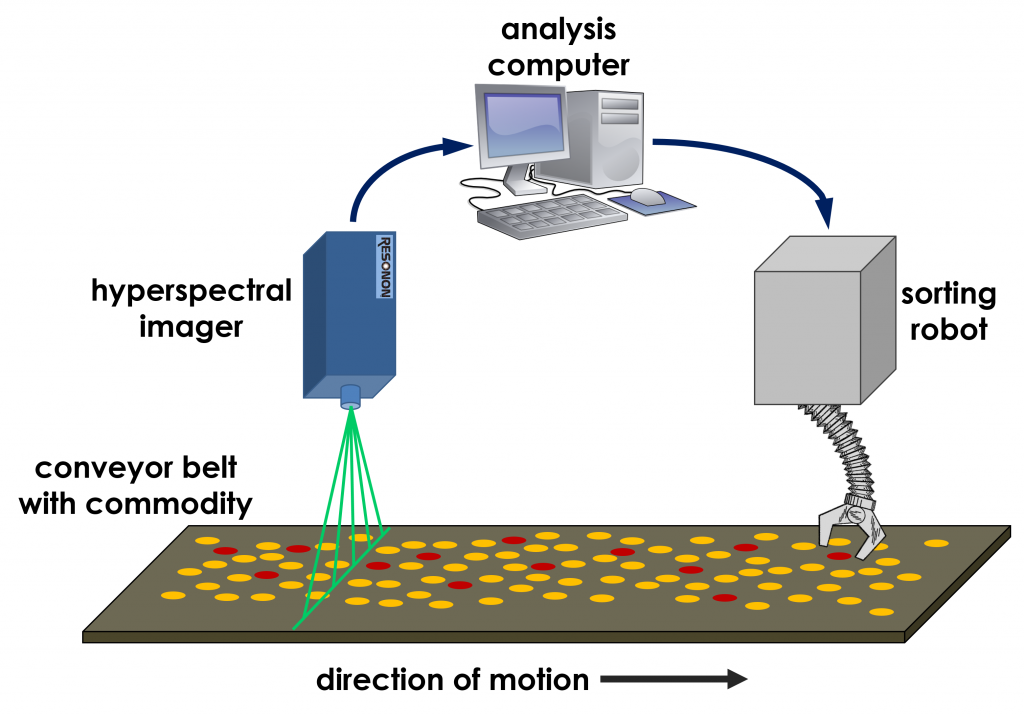
\includegraphics[width=300pt]{images/machine_vision.png}
	\caption{Example of production line using multi-spectral acquisition system with a robotic arm sorting the objects.}
	\label{fig:machine_vision}
\end{figure}

Most production line vision systems have a control mechanism that removes any defected items and allows only acceptable quality to pass. A basic diagram of this process is shown in Figure \ref{fig:machine_vision} whereby a camera provides information to the PC to decide which objects to accept and reject, while a mechanical device removes unacceptable items. This type of system configuration is illustrative of the basic concept of the process, whereas in real applications, the components and peripherals will be much more complex. Vision systems are designed so that the best possible images may be acquired without hindrance from external sources, and is usually very specific to the environment around the cameras, or scene. This may involve specialized lighting (illumination/spectrum), high-power lighting, camera type (high-speed, hyper-spectral, etc.), object sensors, software, visualizations, and many different types of ejection/removal systems.



\section{Industry Partner}

Magnificent Pty. Ltd. is a subsidiary of Berry Yummy Marketing Pty. Ltd. - a strawberry farming and processing company located in Wamuran, Queensland. In this facility (as well as the company's secondary strawberry farm in South Australia), the company plants, grows, maintains, picks, and packs the berries ready for consumer purchase. Berry Yummy Marketing has operated the 100$ha$ farm for over 20 years in Wamuran, and has recently acquired a new, smaller 26$ha$ farm in Myponga, SA. Magnificent employs around 250 people in the peak of the season and consists of planting, picking, packing, driving (tractors/trucks) and operator teams. Producing around 1.7 million $kg$ of strawberries each year, Berry Yummy has a good market share with many high-volume customers including major supermarket chains. The company has it's own transportation and storage facilities allowing for a distribution centre in Brisbane, Queensland's capital city. 

The Strawberries are picked and packed by hand using labour intensive methods in order to produce the finished goods, which can be sold in many different sized packages from 250g through to 3kg jumbo pack. The strawberries are packaged according to the quality grade or cultivar, however, if the fruit is in high demand or weather conditions cause shortages in supply, the lower grades can be used as high grade berries, making the classification depend on market conditions.

\begin{figure}[h]
	\centering
	\begin{subfigure}{.4\textwidth}
		\centering
		
\includegraphics[width=.6\linewidth]{sunray.jpg}
		\caption{}
		\label{fig:sunray}
	\end{subfigure}%
	\begin{subfigure}{.6\textwidth}
		\centering
		\includegraphics[width=.8\linewidth]{whatwedo_logo.jpg}
		\caption{}
		\label{fig:whatwedo}
	\end{subfigure}%
	\caption{(a) Magnificent logo, (b) Workers and fields at Magnificent}
	\label{fig:test}
\end{figure}



Due to environmental and market demands, the standard of strawberries packed can vary between seasons, and as Magnificent employs a mostly casual workforce, the standard can differ between days also. Each operator must pack the correct weight, into the correct container, as fast as possible, whilst ensuring that there are no defected berries from a range of attributes such as over/under ripe, bruising, foreign objects, pest damage, dirt and soil, size, shape and overall appearance. This evaluation can be difficult in this fast-paced environment and could be easily overlooked in situations under pressure, especially when concerned with bruising. Bruising can be hard to detect, even for the trained eye, as the colour and texture takes some time to decay to an unacceptable level. The time taken to decay could be several hours to a few days and, as there may be up to 5 days transport time for berries picked by Berry Yummy, this leads to the case where finished product has left the distribution centre quality assured, but is rejected when it arrives at the destination. Berry Yummy are regularly given feedback from their customers regarding the quality of each punnet after it reaches it's destination point anywhere throughout Australia. Whilst training and education regarding these quality specifications is given, this will be lost as soon as the workforce is replaced by a new season of employees.  

In order to reduce costs and improve efficiencies, Magnificent has invested in various projects to bring a technological approach to farming. Some of these include a strawberry harvesting robot which must navigate through the fields many rows of planting mounds, picking strawberries \cite{busch}. A greenhouse picking system was also developed, where specialised planting troughs were constructed to bring the strawberries to the harvester using a vertical farming method. The company has also connected it's information systems together using a variety of applications interfaced to hardware such as weigh scales and employee clock-in stations. This gives better visibility to the managers and operators to make decisions in a real-time environment. They now have a requirement for an in-line strawberry quality vision inspection system which is capable of inspecting each strawberry in a fast-paced packing environment.



\section{Project Description and Requirements}
\label{sec:requirements}

\textbf{Research Question:} Can packaged strawberries be effectively and accurately quality graded by machine vision on a fast-paced, real time production line?

The concept of this thesis is to develop a system that is capable of assessing pre-packed punnets of strawberries for quality factors such as ripeness, size, rot and mould, bruising, and contaminates. The system must be able to decide between good quality and bad quality, before removing the punnets from the production line for further inspection or discarding. The production line, in it's existing operational capacity, can package two punnets per second, fed from multiple packing stations. The vision system must be designed so that it can be inserted into the current configuration, before the punnets are sealed and palletized, by either replacing existing conveyors or slightly extending the whole production line. The project that this thesis describes was conceived by Magnificent in order to minimize the risk of quality rejections and enhance the fruit's overall appearance on the shelves, and to overcome the aforementioned obstacles.

One of Magnificent's major customers is a nationwide supermarket chain which has a 33\% market share in the fruit and vegetable retail sector \cite{roymorgan}, therefore the quality control of incoming goods are strictly adhered to by receiving personnel to ensure quality standards are met on delivery. If the inspection of individual punnets fail, then the shipment may be at risk of being rejected and turned back to the distribution centre. This return could be as much as 4-5 days transportation and will, in most cases, be unsaleable causing financial loss.

In order to minimize this risk, the quality control of the strawberries must be improved and strengthened by adding a secondary quality control process, utilizing computer vision and image processing methods. The packers will be trained as usual however, their finished punnets will now be additionally assessed by the Strawberry Quality Assurance (SQA) vision system, which is part of the punnet flow in the system outlined in Figure \ref{fig:punnet_flow}. 

\begin{figure}[h]
	\centering
	\includegraphics[width=\textwidth]{punnet_flow.png}
	\caption{Block diagram of the proposed punnet flow.}
	\label{fig:punnet_flow}
\end{figure}

Since 2015, the strawberry packing line has been fitted with a machine that seals the lids on the punnets with plastic film instead of using a resealable lid. This measure has been adopted for a few reasons, namely, cost of packaging, ease of packing, and anti-tampering properties. Shown in Figure \ref{fig:heat_seal}, the heat-seal machine has a maximum speed of 120 punnets per minute or 2 punnets per second, sealing six punnets per cycle, and improving the overall efficiency. Given that the machine must press down onto the stationary punnets with the heating elements, increasing the amount that can be sealed at once, increases throughput rate. However, the length of the heat-seal footprint is correlated to the number of punnets sealed per cycle. As there is limited space, the amount which can be processed simultaneously is also limited. The infeed conveyors must account for this batching of punnets by stopping when the sealing compartment is loaded, and starting when unloaded. The stop-start action is suppressed by an accumulator conveyor running at a slower speed and gradually feeding into the batching section, but still requires the infeed to stop, albeit at a lesser frequency. This means when integrating production conveyors to feed this machine, the discontinuous nature of the flow of punnets must be considered.



\begin{figure}[ht!]
	\centering
	\begin{subfigure}{\textwidth}
		\centering
		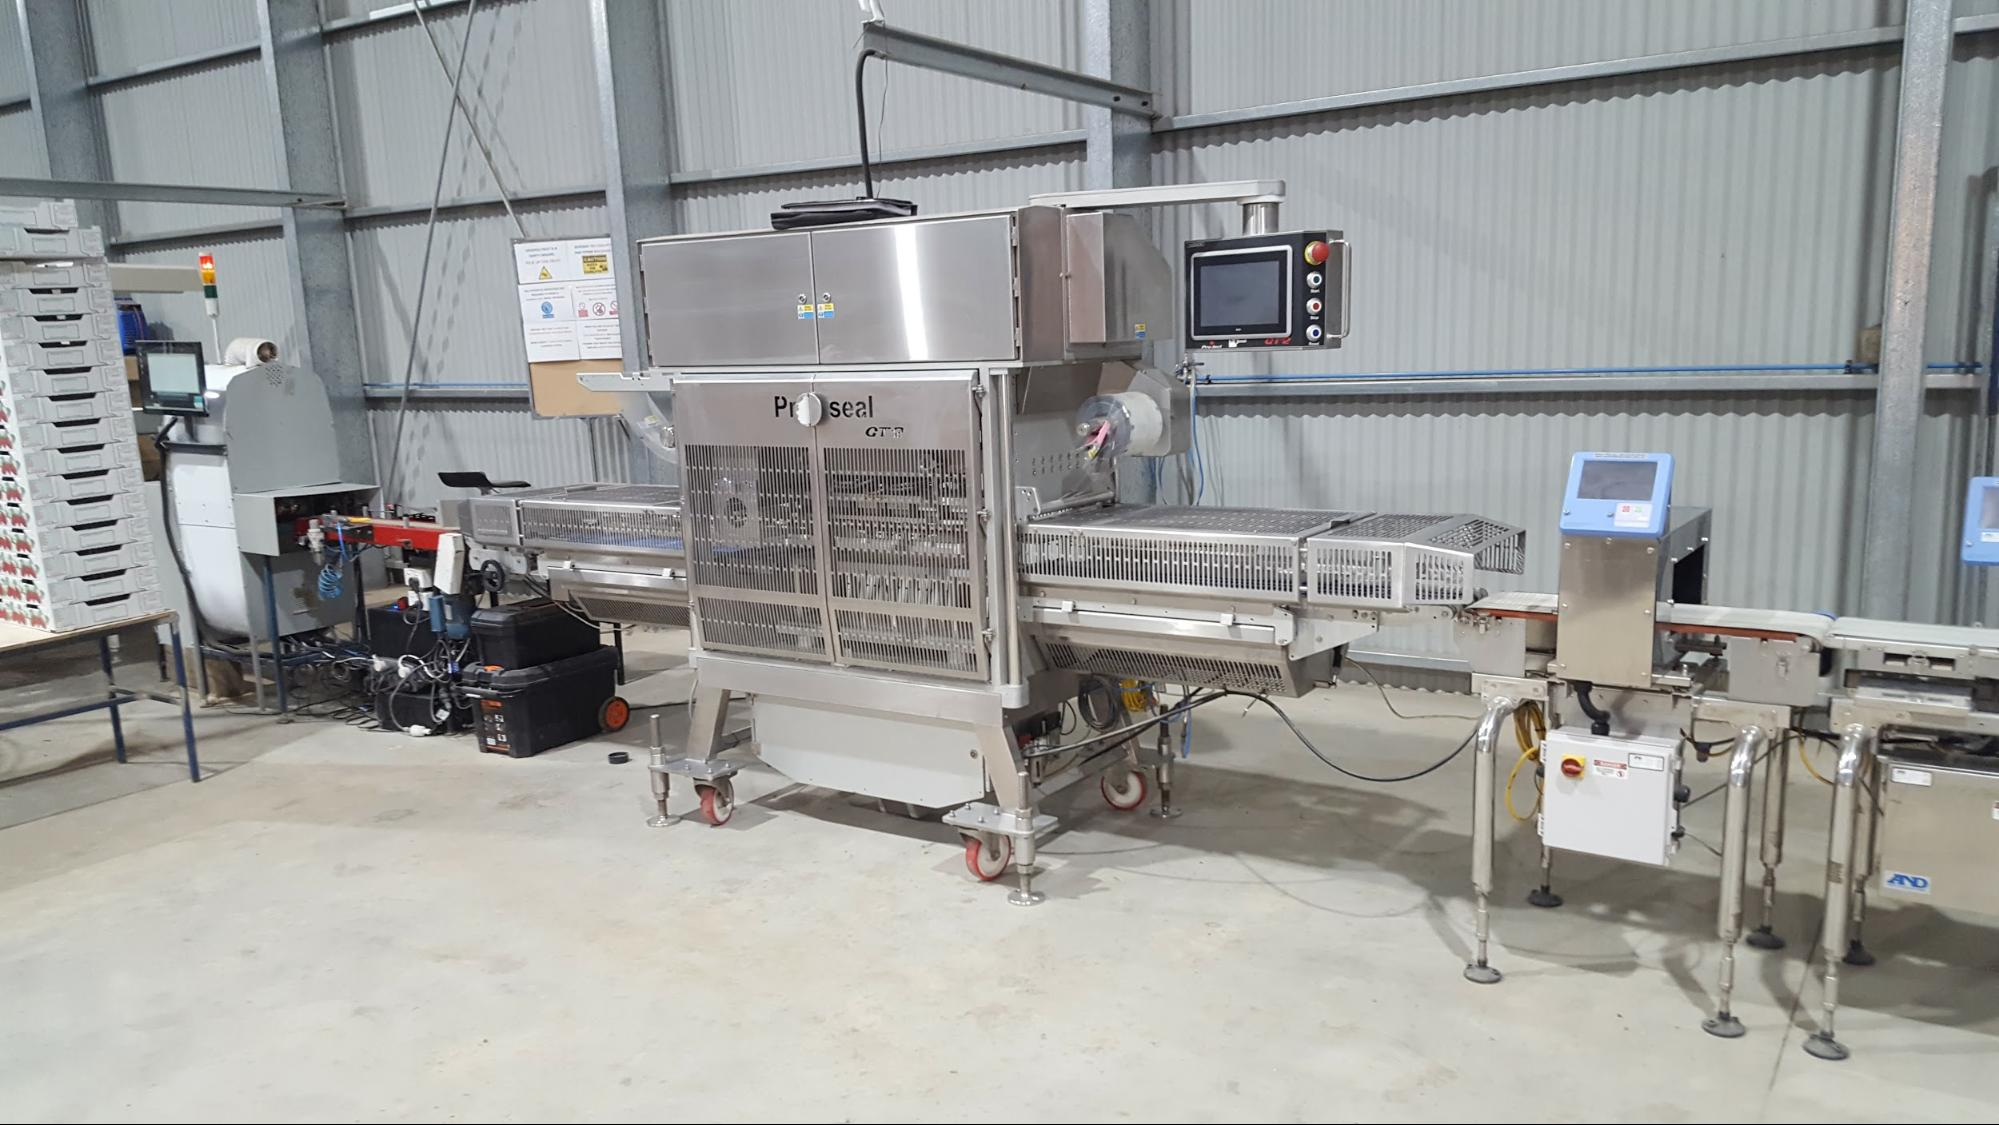
\includegraphics[width=.8\linewidth]{heat_seal.jpg}
		\caption{}
		\label{fig:heat_seal}
	\end{subfigure}%
	
	\begin{subfigure}{.5\textwidth}
		\centering
		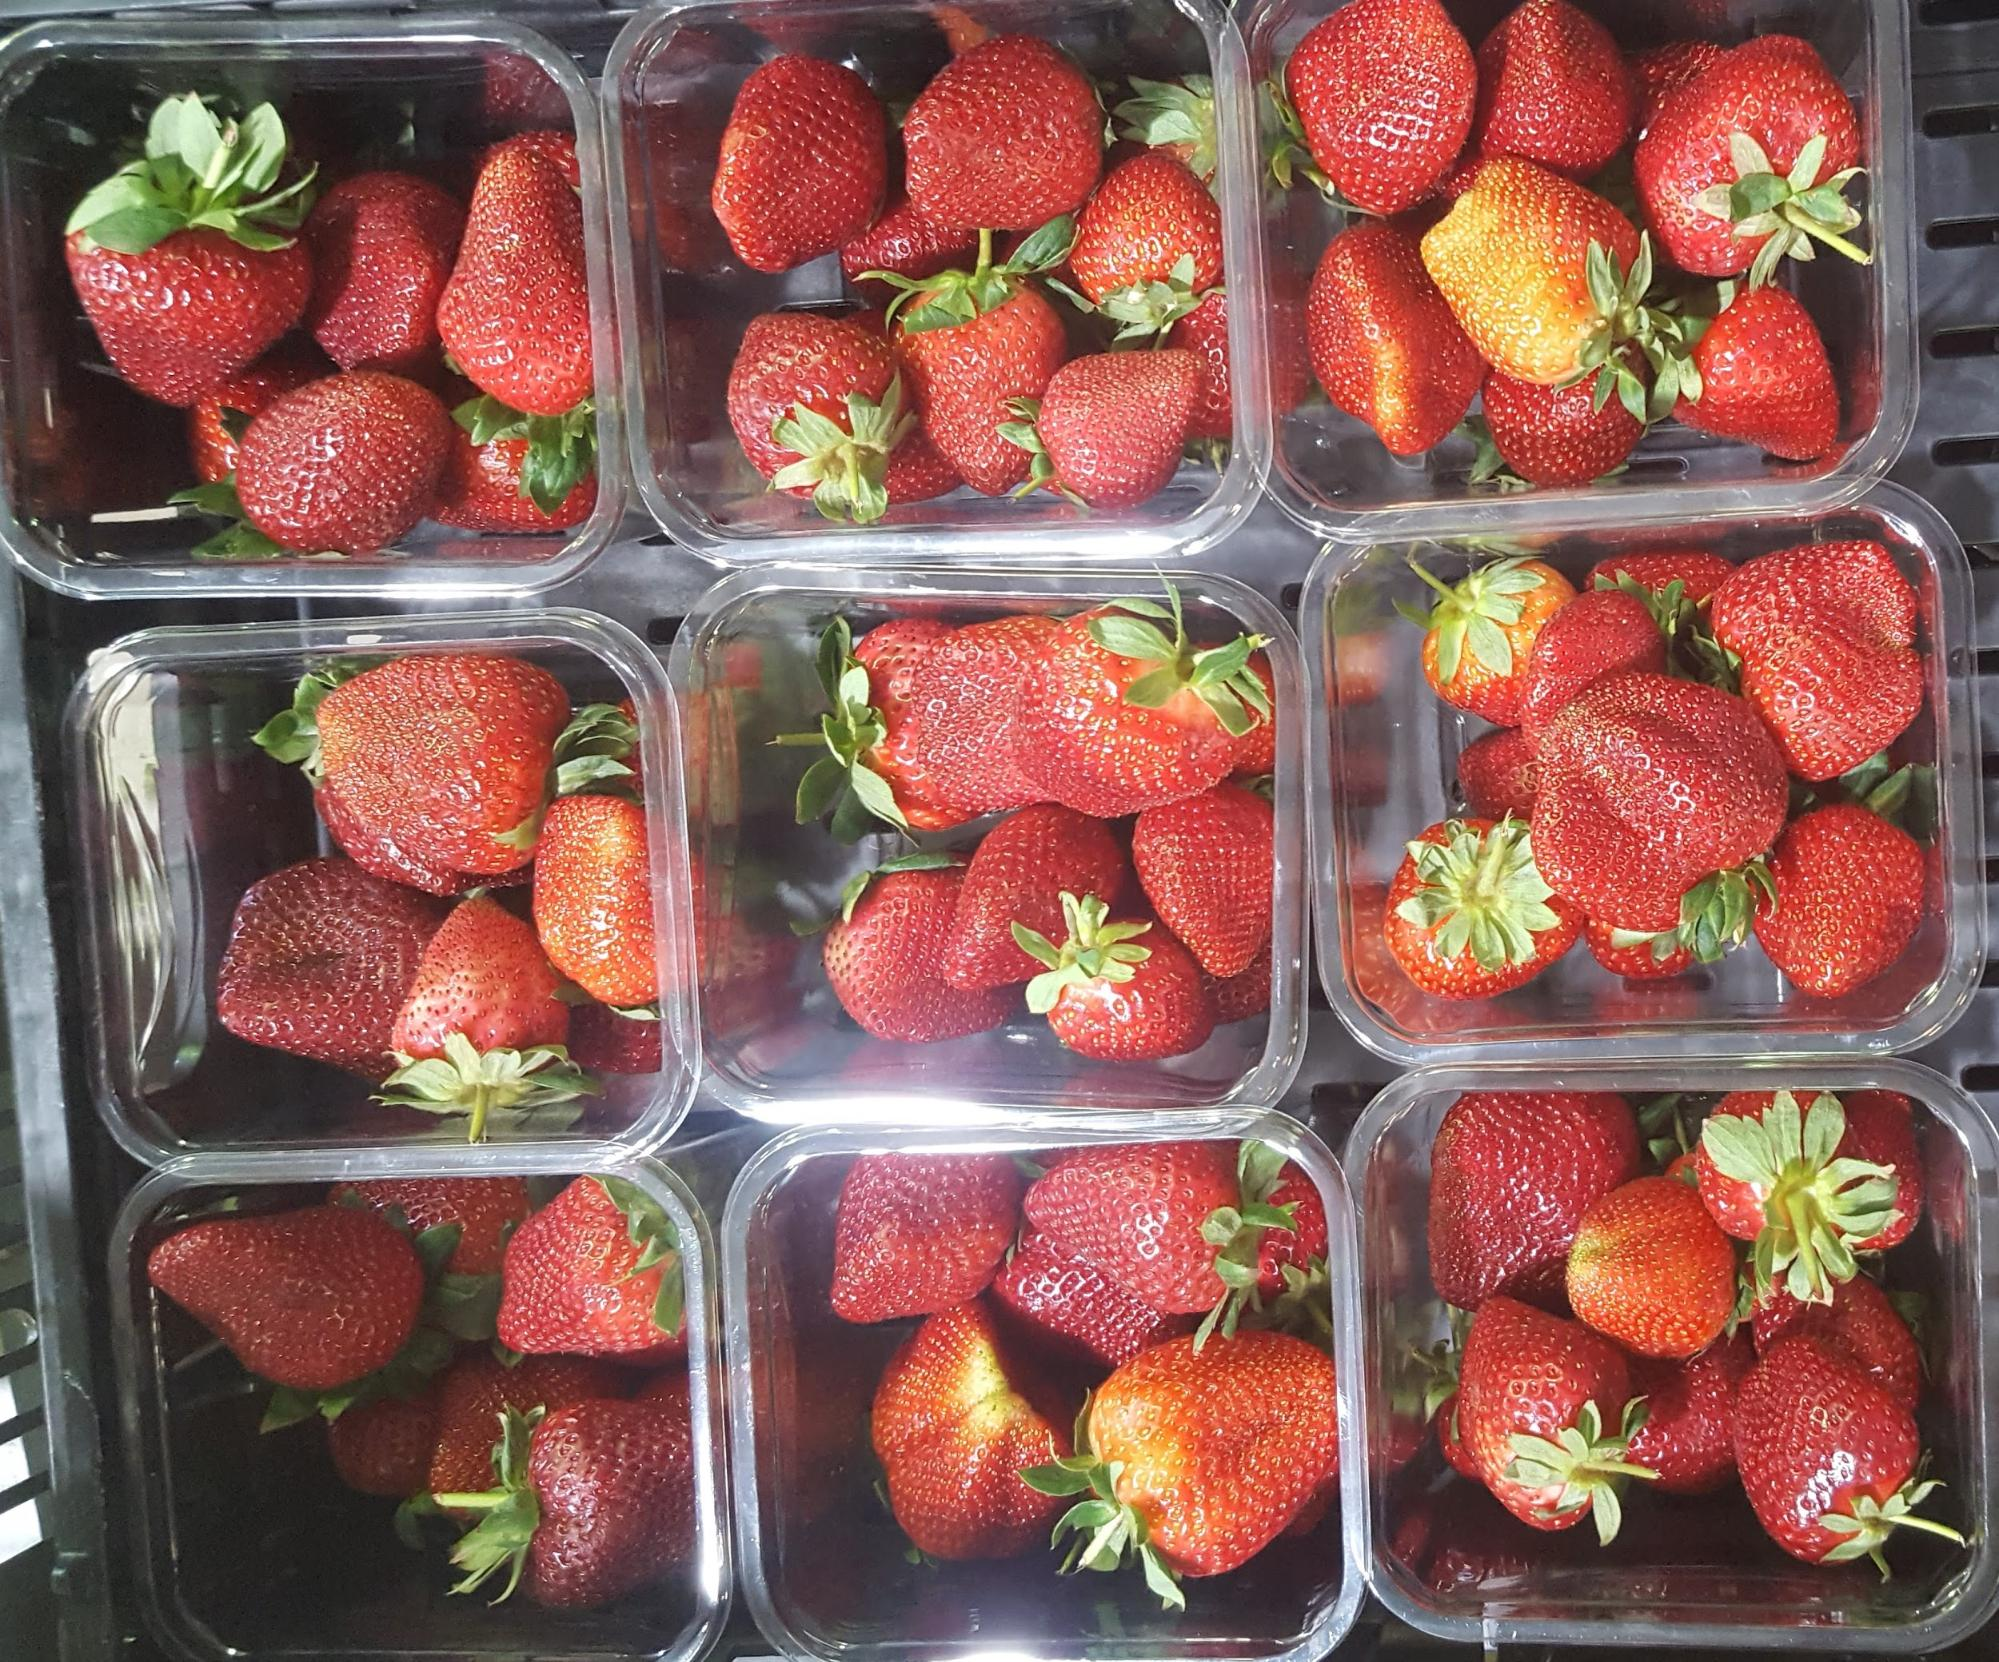
\includegraphics[width=.6\linewidth]{unsealed_punnets.jpg}
		\caption{}
		\label{fig:unsealed_punnets}
	\end{subfigure}%
	\begin{subfigure}{.5\textwidth}
		\centering
		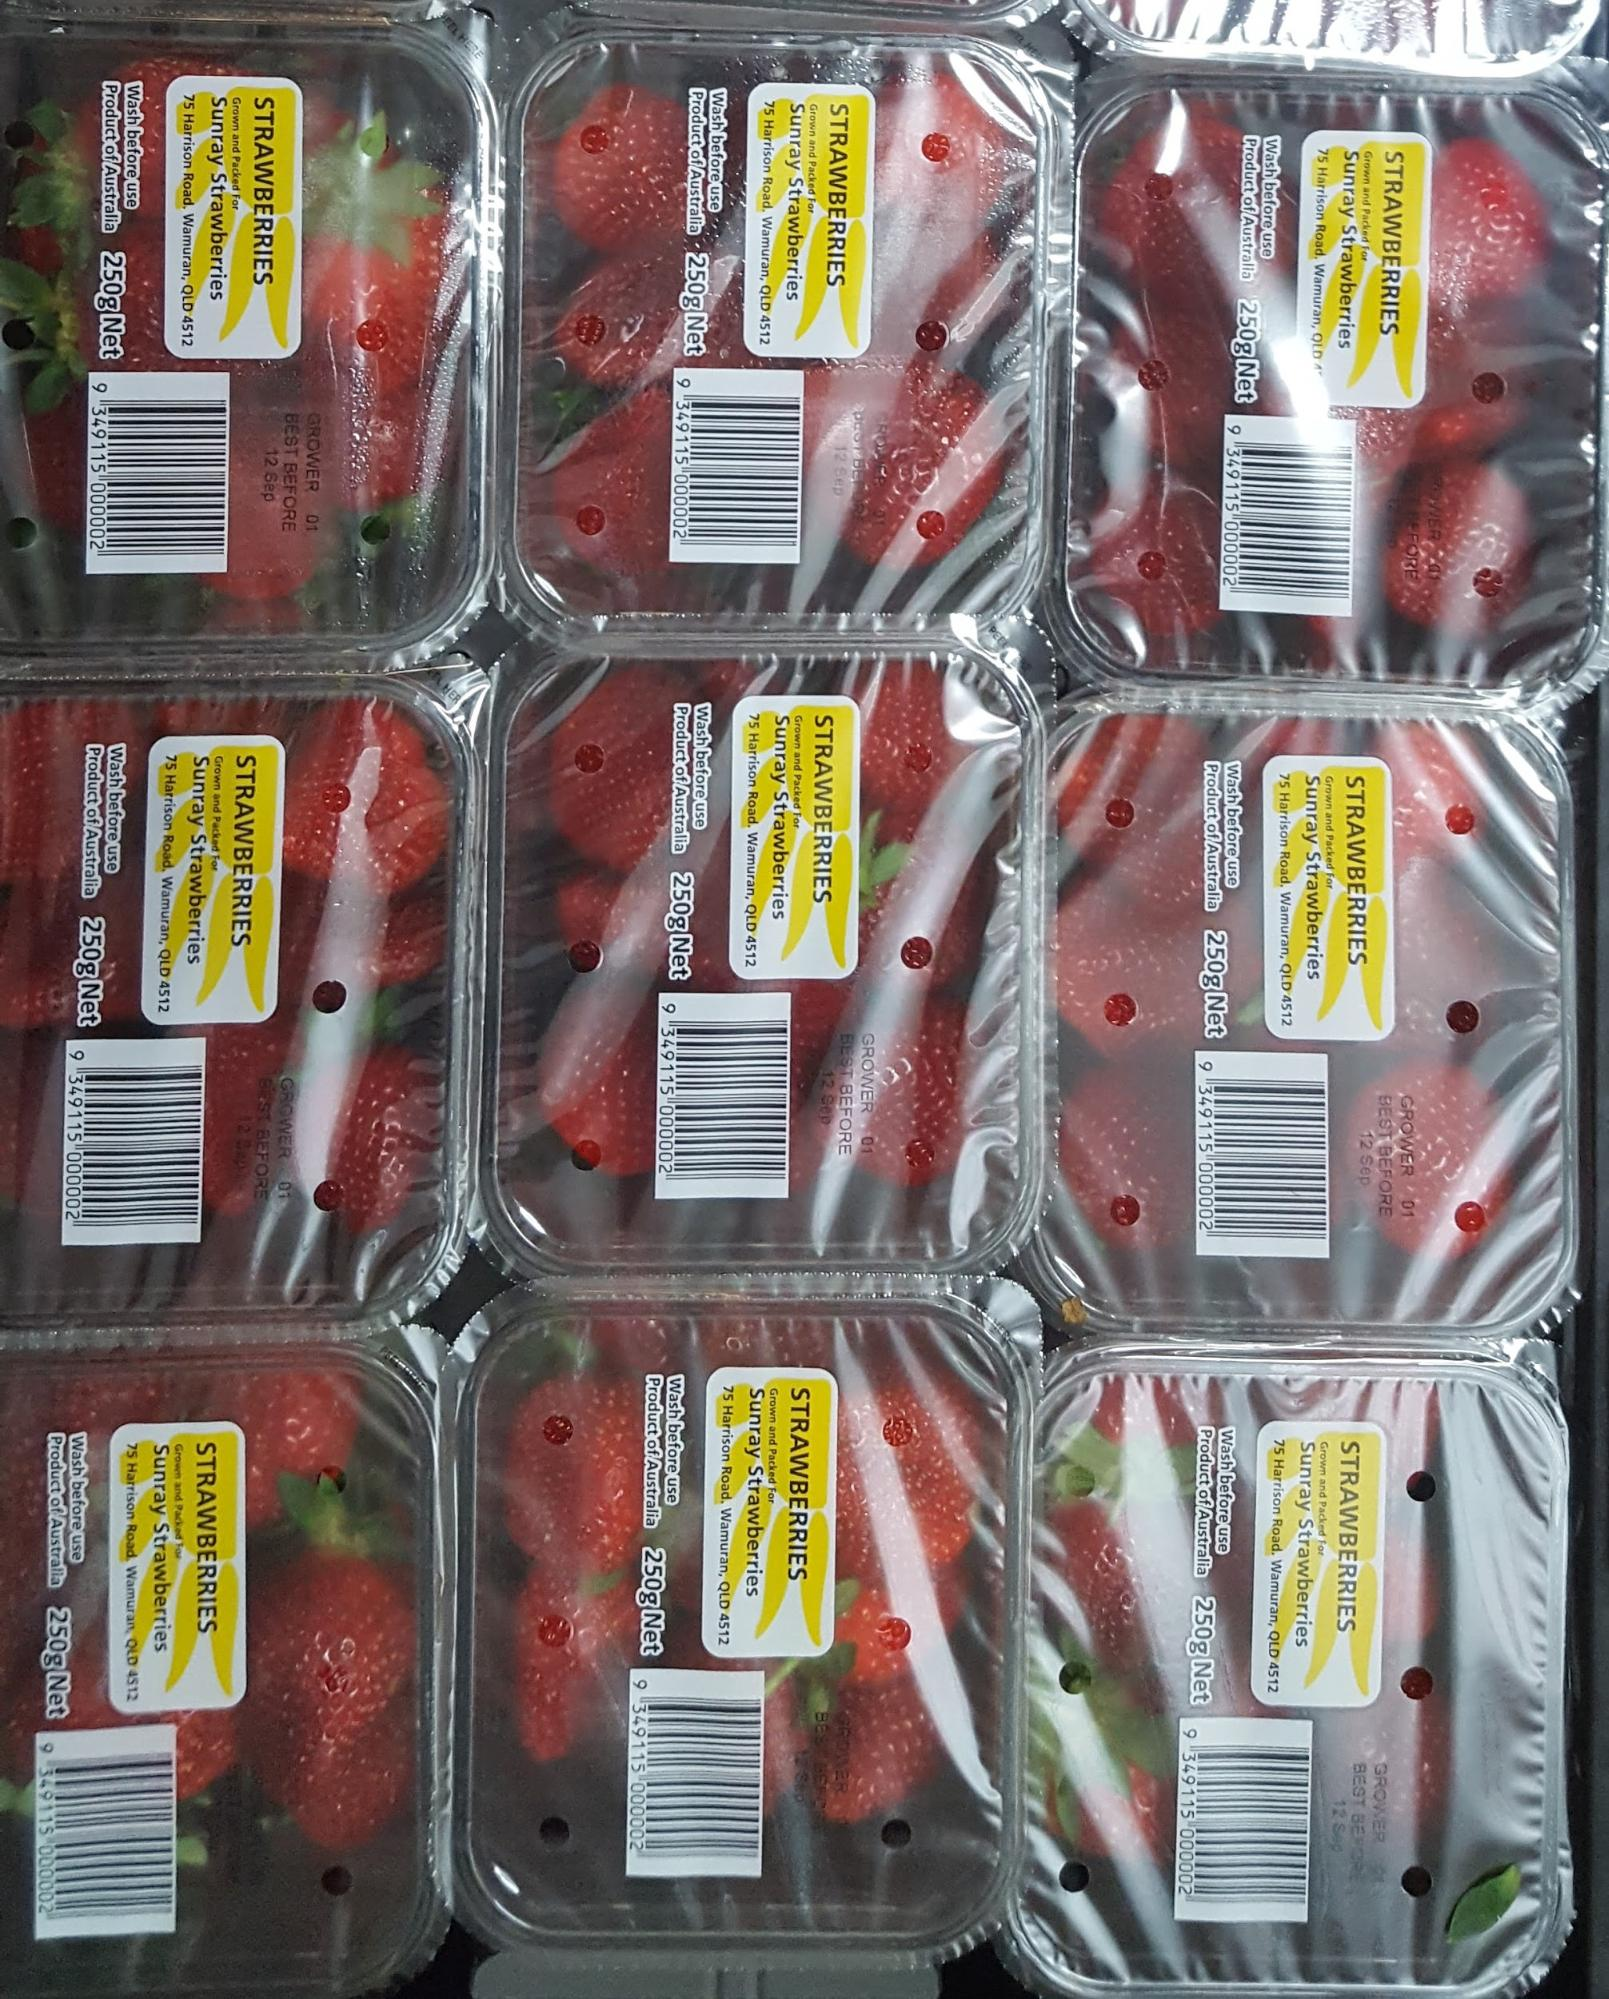
\includegraphics[width=.5\linewidth, angle=90]{sealed_punnets.jpg}
		\caption{}
		\label{fig:sealed_punnets}
	\end{subfigure}%
	\caption{(a) Heat-Seal machine, (b) Punnets before sealing, (c) Punnets after heat-sealing.}
	\label{fig:HS}
\end{figure}



Thin film rolls are used to supply the heating dye with material to press and seal around the edge of the punnet, discarding the excess onto another roll. The pre-sealed and post-sealed punnets are shown in Figures \ref{fig:unsealed_punnets} and \ref{fig:sealed_punnets} and present a unique method to tamper-proof each punnet. The film, once removed, cannot be re-sealed giving consumers the confidence that each punnet has not been opened since it was packed. After being sealed, each item is passed through a metal detector, and a weight-checking scale. At both of these checkpoints, the punnets can be ejected from the production line using pneumatic air actuators.

The addition of a vision system to the heat-seal infeed is the desired outcome for Magnificent to address quality issues that can be missed in such a fast-paced environment. Defects such as under ripe, over ripe, bruised, rotten, foreign object and size and shape have all been attributed to stock rejects and/or returns. As it can cost more to salvage rejected stock than reuse it, there is a possibility that poor quality could mean a shipment is subject to dumping. As millions of full punnets are packed, palletised and shipped each year the Quality Assurance Manager has an enormous, if not impossible, task in inspecting each one thoroughly. Strawberries are required to be picked and packed to a strict set of attributes, however, subjectivity, general tiredness, rushing to perform tasks, and overheating of workers can all influence the quality of berries picked in the field or packed on a production line. Subjectivity is of great concern due to the high turnover of staff, given the majority of employees are seasonal workers, only a few of which will return each year. Therefore, the vision system will inspect each punnet from the top and bottom, at high speed, adding objective consistency to the process as one of the final quality steps before palletizing and shipping.


The requirements include that the vision system feed directly into the heat-seal machine, and not inhibit the production speed or volume. This is a critical measure, particularly during development and production line integration, which ensures that efficiencies are not lost in packing. The speed of packing punnets is directly related to the profit of both the company and its workers, both of who's income is proportional to volume over time. The company loses money paying for workers to wait for machinery to be ready, hence, downtime due to a non-critical plant will be counter-productive and should be avoided. The inspection system must be able to detect the incoming, high-speed punnets and acquire images from above and below, before analysing the quality. If the system detects defects in the strawberry images, the punnet must be removed from the production line. 



The vision system general requirements are listed in Table \ref{tab:requirements} showing other critical success factors.



\renewcommand{\arraystretch}{0.8}% Tighter table height
\begin{longtable}{p{2.5cm}p{12cm}}
	\caption{Table of Major Requirements for the Strawberry Vision System}
	\label{tab:requirements} \\
	
	\hline\hline
	\textbf{Requirement} & \textbf{Details} \\[2pt]
	\hline \hline
	\textbf{\textit{Continuity}} 	& - Must not inhibit the production line speed. \\[2pt]
	& - The production line should not be caused to stop unnecessarily due to the vision system.\\[2pt]
	\hline
	\textbf{\textit{Safety}}    & - The vision system shall not create any safety risks or hazards such as tipping, electrocution, exposed pinch points, sharp edges, hazardous lighting, unsustainable lifting, etc.  \\[2pt]
	\hline
	\textbf{\textit{Inspection}} 	& - Autonomous operation.\\[2pt]
	& - The punnets are to be assessed based on the agreed defect categories (classes) to the specifications provided. \\[2pt]
	& - Each punnet will be evaluated from top and bottom (through the plastic container). \\[2pt]
	& - The infeed and outfeed systems integrate with the proceeding and preceding machinery. \\[2pt]
	\hline
	\textbf{\textit{Footprint}}	& - Shall be externally connected to either one $400VAC$ or $240VAC$ power source, and one pneumatic line for all operations including removal from production line.  \\[2pt]
	& - Adaptability to multiple production lines. \\[2pt]
	& - Size of the system shall be kept as compact as possible due to packing room constraints. \\[2pt]
	\hline
	\textbf{\textit{Outputs}}	& - Defective punnets will be ejected from the production line.  \\[2pt]
	& - Operational statistics will be presented to help the operator make decisions based on performance.  \\[2pt]
	& - Light and sounds shall accompany the system to be intuitive to operators \\[2pt]
	& - Error, success, and general information shall be presented on a screen, or given to operators via another medium.  \\[2pt]
	\hline
	\textbf{\textit{Traceability}}		& - Records to be kept with each punnet's images as to when (date/time) they were packed.  \\[4pt]
	& - Images, timestamp, assessment, system state, and other records must be kept in a database for future access. \\[2pt]
	\hline
	\textbf{\textit{Documentation}}	& - Each software module is required be documented to describe the module and it's function and relevance to the application.  \\[4pt]
	& - A description of how the software is compiled and which dependencies are required to run the application will be provided. \\[2pt]
	\hline
\end{longtable}


Systems failing to add value to a production line are typically adopted only for a short time, if at all, due to problems such as low throughput \cite{brosnan, liming}, unacceptable error rates \cite{matteoli, elmasry2}, and complex acquisition processes \cite{liu2, chiu}. Slowing down or stopping the production line financially impacts both the producer and the workers in terms of wasted time. The producer's costs reduce ($\$/kg$) and the worker's pay reduces ($\$/hr$), if the throughput reduces, therefore the optimal solution involves the most rapid process to perform the packing, and any time hindrance would be seen as an inefficiency. 

Errors can be either false positives (FP) meaning a sound item rejected, or false negatives (FN) meaning defect item passed. If there are too many FN occurrences, the consumer will see no change in the quality of produce, however if there are too many FP occurrences, the operators will have to perform double handling duties in an already fast-paced and high-pressure environment. Therefore, the approach used to ensure adoption into production will be to reduce FP instances as much as possible in the first instance, even if this means a lower overall accuracy initially, before improving the FN rate.  



\section{Contributions}



Due to the unique requirements of the candidature in conjunction with an industry partner under the Australian Research Council (ARC) Linkage program, the fulfilment of this thesis is largely based on the successful application of novel systems. In contrast to theses which are based on generalised approaches to common problems, this work is bound to a specific set of requirements and continuous real-world implementation of the research and development performed. The project detailed in the following chapters has been the sole focus for the entire candidature period, building a platform for the university to foster growth, relationships, and reputation within the agricultural industry and community.


Research and development performed during the undertaking of this project has contributed the following benefits in terms of production line application, agriculture, and industry partnerships:

\begin{itemize}
	\item Research and experimentation into production-level lighting quality shows that consistent, completely diffuse, cross-polarised illumination capable of removing all specular reflections (whilst maintaining fine-grained features) is achievable.
	\begin{itemize}
		\item Published paper presented in Chapter \ref{sec:paper_1}.
	\end{itemize} 
	\item Colour analysis techniques used to determine under and over ripe strawberry defects on a fast-paced production line.
	\begin{itemize}
		\item Published paper presented in Chapter \ref{sec:paper_2}.
	\end{itemize}
	\item Driving innovation and adoption of state-of-the-art techniques within industry, and partnerships with university research teams:
	\begin{itemize}
		\item Project success used as evidence in approval of state-of-the-art agriculture and aquaculture research hub within the university. - TODO - add details??
		\item Herald Sun article and promotional material produced by the university provide publicity and awareness for institutions and industry. - TODO - more articles??
	\end{itemize}
	\item Integration and deployment of novel, scalable, real-world machine vision systems in an industrial setting, in order to drive productivity and reduce overall costs to producers.
	\begin{itemize}
		\item More than 5000 punnets have been identified as defective and re-packed or removed from the production line, avoiding costly potential stock returns, and diminished reputation.
		\item Objective, consistent inspection of produce allows operators to finely-tune quality sensitivity settings according to market conditions.
		\item Provides ability to operators for immediate quality control feedback to packing staff.
		\item Traceability of physically timestamped punnets to database timestamped images allow accurate comparison of customer complaints to packing condition investigations.  
	\end{itemize} 
	\item Confirmed the validity of grading post-packaged strawberries, opposed to singular, increasing throughput potential and reducing damage by human handling.
	\begin{itemize}
		\item Proven application of controlled illumination and continuous acquisition of packed strawberries on an high-volume process line. 
		\item Asynchronous processes ensuring multiple acquisition, processing, display, and control functions occur when required.
		\item Image processing and deep learning models capable of inference within required time window of $500ms$.
		\item F1 accuracy of $94\%$, $89\%$ and $90\%$ for image processing, and ROC scores of $87\%$, $80\%$, and $58\%$ for deep learning models have been obtained for classification of under ripe, foreign object, and over ripe punnets, respectively.
	\end{itemize}
	\item First production-scale, in line strawberry quality inspection system.
	\begin{itemize}
		\item Commercial inspection of full punnets of berries, rather than the much more inefficient singulated versions seen in research articles and experimental systems. 
	\end{itemize} 
	\item Production deployment of deep learning models to evaluate fast-paced strawberry punnets.
	\begin{itemize}
		\item Pre-trained Resnet 50-layer network used to extract feature vector before a logistic regression classification process. 
		\item Single binary models for each class allow adjustable sensitivities catering for changing seasonality and conditions.
	\end{itemize} 
\end{itemize}







%%%%%%%%%%%%%%%%%%%%%%%%%%%%%%%%%%%%%%%%%%%%%%%%


\section{Thesis Outline}

The thesis is arranged such that an in-depth literature review is presented, which looks at industry methods in terms of agriculture and machine vision from a theoretical and applied point of view, and following chapters describe the research, development, experimentation, and results of the vision system configurations and it's transition to production-ready. Finally, we look at the implementation of machine learning algorithms in order to progress toward deep learning in real-time.  

The body of this thesis is set out with the following chapters: 


\begin{itemize}
	\item \textbf{Chapter \ref{sec:lit} - Current Industry Methods and Review of Literature:} A review of industry standards and state-of-the-art methods for a range of applications in relation to produce grading, classification, or processing using machine vision. 
	
	\item \textbf{Chapter \ref{sec:I} - Strawberry Inspection System Design:} Research, design, and development of components and systems required to perform multiple fast-paced acquisitions and image processing of each punnet. Included are considerations for  safety and control systems, lighting configurations, power requirements, software packages and frameworks, high-speed imaging, and ejector mechanism synchronisation, as well as the construction of a prototype enclosure, providing much of the groundwork and development for the production version. 
	
	\item \textbf{Chapter \ref{sec:paper_1} - A Method to Create Stable Lighting and Remove Specular Reflections for Vision Systems:} Conference paper with poster presentation at DICTA 2017 detailing the solutions to remove specular reflections using cross-polarisation, and creating stable DC lighting when using high-speed photography.
	
	\item \textbf{Chapter \ref{sec:II} - Production Integration:} Moving from bench design to production line required efficient, unobtrusive, and seamless integration to the already existing process line. The migration of systems into production was designed in order to have minimal impact on the flow of produce. Pre-built components tested before final installation, including punnet control mechanism, allowed rapid transitioning. Production data, image processing algorithms are discussed as well as maintenance limitations discovered in the design.
	
	\item \textbf{Chapter \ref{sec:paper_2} - Colour Analysis of Strawberries on a Real-time Production Line:} Conference paper with oral presentation and CiSRA award at DICTA 2018 showing the colour-based image processing techniques used to determine under and over ripe features during full speed production. 
	
	\item \textbf{Chapter \ref{sec:III} - Systematic Reconfiguration Toward a Robust Production Environment Design:} Improved maintenance and cleaning designs of cameras, lighting, power systems, polarisers, and electronics is presented along with improved lighting configuration, reducing power consumed and heat produced. Standardisation of microcontrollers finalises the upgrade which is performed inter-season in order to have minimal down-time, with further production data captured in the two seasons following.  
	
	\item \textbf{Chapter \ref{sec:IV} - Machine Learning Approach to Grading Strawberries:} Machine learning and deep learning methods required software environment changes to enable open source libraries and packages to be used rather than remote cloud or local wrapper options. Preliminary test results reported excellent results before experimentation with Resnet pre-trained deep network and Logistic Regression to create a strawberry classification model.  
	
	
\end{itemize}




%%%%%%%%%%%%%%%%%%%%%%%%%%%%%%%%%%%%%%%%%%%%%%%%%%%%%%%%%%%%%%%%%%%%%%%%%%%%%%
%%%%%%%%%%%%%%%%%%%%%%%%%%%%%%%%%%%%%%%%%%%%%%%%%%%%%%%%%%%%%%%%%%%%%%%%%%%%%%
\newpage

\chapter{Current Industry Methods and Review of Literature}
\label{sec:lit}

Production lines adopt computer vision systems in order to reduce the cost of labour and/or standardise the quality control. Depending on volume and product, quality controllers may be a substantial cost in production and can be subjective, particularly for seasonal work. This leads to loss in productivity, labour costs, and financial loss in the form of stock returns, in the case that it is not accepted by the customer. Employing accurate vision systems on a production line give the producers quality control that is consistent, continuous, and relatively cheap \cite{heleno,chen}. 

Performing a review on fruit Cubero et al \cite{cubero} investigated Apple, banana, citrus, cucumber, mango, mushroom, olives. potatoes, star fruit and watermelon as part of their investigation into agricultural machine vision. Methods such as colour analysis, histogram, k-NN, PCA, Fourier analysis, clustering, AdaBoost, and ANN's to perform the tasks of inspecting a wide range of defects and classifications. Another review by Dubey and Jalal \cite{dubey} investigated two types of tasks for vision systems - classification and defect detection - and concluded that most of the work in this field contained three steps in performing either task, namely, background subtraction, feature extraction, and training and classification. SVM, BPNN, Decision Tree, ANN, and even fusion classifiers were commonly used in their research.

As the field of production line machine vision in general has a wide spectrum of applications, the following literature review will only concern agricultural machine vision. 


\section{Image Processing in Produce Grading}

 
The use of simple techniques have been implemented in produce grading due to the inherent properties such as colour (ripening, defects), and texture (disease, freshness) extraction and analysis. Significant findings in experiments have led to vision systems adopting simple methods such as morphology, thresholding, fuzzy logic, colour space transformations, and edge detection (or a combination) to successfully detect or classify produce to an acceptable level or, in some cases, improve on more sophisticated processes.

Common colourspace transformations for colour grading and defect detection include HSV and CIE-Lab (Figure \ref{fig:colour-space})due to their specialised colour channels and properties. Work has been sampled by Pathare, Opara, and Al-Said \cite{pathare} in their review of colour measurement and analysis performed in order to evaluate fresh foods. They reviewed items including red table grape, tomato, orange, apple, banana, chicken breast and varied meat, flour, pasta, cereals, and breads all of which used a colour index (CI) to perform quality checks. They all had the commonality in that they used mathematical operations with coefficients relating to one or more colour spaces such as HSV, CIE-Lab, and CIE-XYZ. These colour indexes were used to make a comparison against test samples for characteristic representation of maturation, preservation, or storage. 

\begin{figure}[h]
	\centering
	\begin{subfigure}{.5\textwidth}
		\centering
		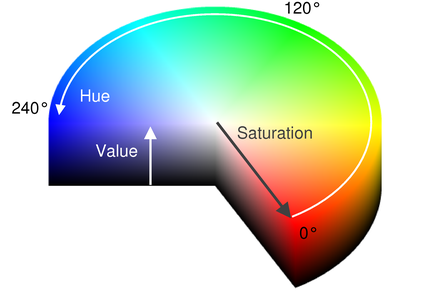
\includegraphics[width=.7\linewidth]{hue_sat.png}
		\caption{}
		\label{fig:HSV}
	\end{subfigure}%
	\begin{subfigure}{.5\textwidth}
		\centering
		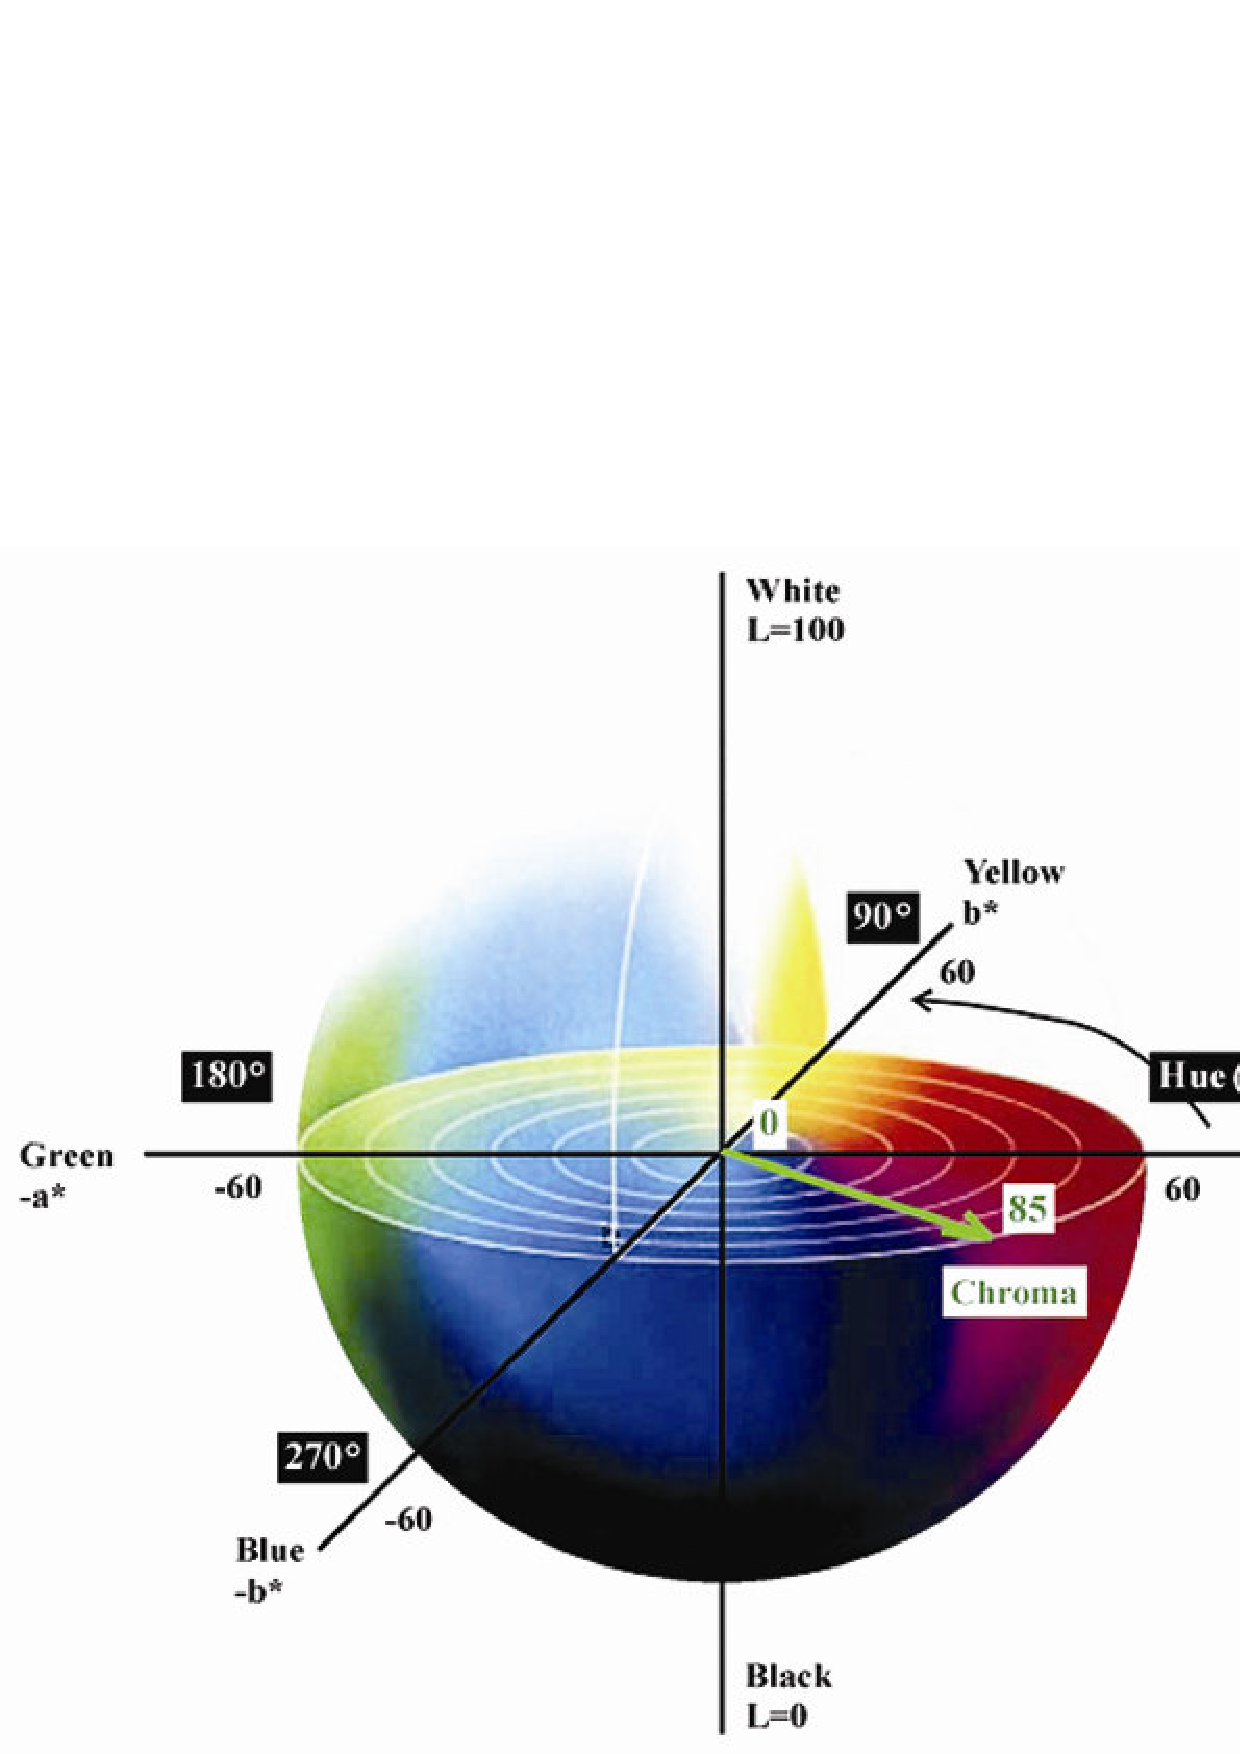
\includegraphics[width=.9\linewidth]{CIELab-colour-space.png}
		\caption{}
		\label{fig:Lab}
	\end{subfigure}%
	\caption{Colour spaces (a) HSV and (b) CIE-Lab.}
	\label{fig:colour-space}
\end{figure}

Two species of table grape were graded into five categories by Cavallo et al \cite{cavallo} after training a Random Forrest Classifier with features from the CIE-Lab colour space. The team calculated the mean and standard deviation of each channel and added the product of channels and ratio of channels to achieve a $92\%$ and $100\%$ cross-validation accuracies for Victoria and Italia strains, respectively.

A method to grade lemons based on colour and volume was implemented by Khojastehnazhand, Omid, and Tabatabaeefar \cite{khojastehnazhand} where the system could be calibrated to the specific requirements before assessment begins by passing fruit as examples to the system (and stored in a database), before using the example data as comparison to the unseen fruit. The colour and volume information was calculated via HSI colourspace and simple geometry measurements where the volume estimation $R^2 = 0.9852$ and colour (ripeness) estimated accuracies of $95.45\%$, $100\%$, and $86.67\%$ for classes 1, 2, and 3, respectively.

For many leafy vegetables green is the predominant colour, therefore, extraction of the healthy components is made easy using the above-mentioned colour spaces. In order to identify leafy vegetables Danti, Magdi, and Anami \cite{danti} utilised the RGB and HSI colour space channels by simply finding the mean and range (variance was eliminated as a non-determining factor) of each channel as features. The features were used to train a BPNN model which scored in the range of $92-100\%$ for all 10 leafy vegetables including dill, fenugreek, coriander, spinach and mint. 

RGB or a combination of RGB with other colour spaces also give significant results for certain applications. In order to grade palm oil fruit, May and Amaran \cite{may} simply analysed the RGB range of under ripe, ripe and over ripe fruit colour and determined associated values correlating to the ripeness. Their fuzzy logic system achieved an overall accuracy of $86.67\%$ showing that this method is plausible for fruit ripeness determined by colour. A method to grade four different varieties of mango into four ripeness grades was implemented by Nandi, Tudu, and Koley \cite{nandi} by extracting colour features, and deriving other colour features at key points across length of the fruit. The features were then used with a simple Gaussian Mixture Model (GMM) to achieve accuracies that rivalled expert humans. Blasco, Aleixos, and Molto \cite{blasco2} developed an algorithm that can detect 12 different types of common disease in citrus fruits. The method reduces the image to 32 colours before performing a region-growing method and could assess fruit from different batches, and even species, of citrus without adjustments. This was based on the assumption that unaffected fruit peel is relatively consistent, smooth, and blemish-free. An overall accuracy of $94\%$ was attained with some of the most devastating diseases scoring $100\%$ detection. 

Geometric calculations are a common approach to assessing shape, size, or volume as the scale and intestine are invariant which facilitates the background removal process, leaving a precise outline. This outline can then be accurately measured due to the fixed position of a calibrated camera. Properties such as minor and major axis can be used to calculate area (size) and lenth-to-width (elongation) of objects. Contour curvature, shape matrices, moments, and shape transforms such as Fourier and Wavelets can also be calculated from a well segmented image. 

Sandrina et al \cite{sandrina} implemented a method using geometric calculations to determine weight and shape of watermelons. Using logistic regression analysis they determined that good specimen shape could be well-described by an ellipsoid model with an $R^2$ of $0.97$. The weight of the watermelons was estimated by image analysis with an error of $2.42\%$. A review of assessment techniques for legume quality was conducted by Mahajan, Das, and Sardana \cite{mahajan} that found several species including lentils, soybeans, peas, chickpeas, beans, and honeylocust were assessed for their geometrical properties such as size and shape. Using a flatbed scanner for each of these projects, the methods consisted of simple thresholding and morphology to find the binary image before measuring. 


Fuzzy systems can offer generalisation and adaptability properties for grading based on feature simplification. A Fuzzy Inference System (FIS) takes raw data (crisp), transforms it into a simplified version (Fuzzification), and makes a prediction based on some knowledge, before transforming again (De-Fuzzification) back into a crisp value. Fuzzification methods may include bucketing, averaging, PCA, or windowing in order to reduce the dimensionality of data, usually giving the ability to assign simple rules to perform the classification or detection.

Hasan and Monir \cite{hasan} developed a system to evaluate guava by use of a FIS. The fuzzy rules were based on functions of hue, saturation, and intensity of the images acquired of the fruit. Their method achieved an accuracy of $93.4\%$ which is an improvement over other classifiers such as naive Bayes and multi-SVM. A method that used volumetric estimation in order to perform quality grading in fruit (apples, mango, orange, pomegranate, and strawberry) was designed by Jadhav, Singh, and Abhyankar \cite{jadhav}. Four cameras positioned at various angles and elevations were used to acquire the calibrated images of fruits before the volumetric calculations were performed. This information is coupled with the colour values from the hue channel of HSV colour space to obtain a classification grade which is then passed to an FIS for final distribution into five grades from very poor to very good. All grades and all fruits achieved accuracies of $>98\%$. 

An adaptive neural-fuzzy inference system (ANFIS) has been developed by Zheng, Jiang, and Lu \cite{zheng} in order to detect bruising in Chinese bayberries as a function of Fractal Dimension (FD) and RGB values. The multiple input, single output Takagi–Sugeno fuzzy network consists of an input layer, fuzzification layer, rule layer, defuzzification layer, and output layer. The trained network could discriminate between bruised and unbruised bayberries with an overall $90\%$ accuracy. Similarly, Jiang et al \cite{jiang} used an ANFIS to predict ascorbic acid retention in fresh-cut pineapples They used inputs of surface area, storage temperature, and storage time in order to train the predictor with a RMSE of $7.88\%$ and and $R^2$ correlation coefficient of $0.95$.

Goel and Sehgar \cite{goel} developed a Fuzzy Rule Based Classification System (FRBCS) in order to grade tomatos into six ripeness stages. Images acquired from the open farm environment were preprocessed by taking averages of R, G and B, R-G and R/G before training and testing, with comparisons against Naive Bayes, SVM, MLP, and Random Tree classifiers. Their method of FRBCS achieved an accuracy of $94.29\%$ which outperformed the others ($88.89\%$, $87.42\%$, $84.97\%$, and $84.05\%$, respectively).  




\section{Hand-selected Features}

The process of hand-selecting features is a common approach to help classifiers or networks to focus on the most important characteristics which determine class or defect. If the feature is a known conditional variable for the application then it can be a simple matter of extraction. For example, a particular fruit may have a distinctive disease indicator such as black spots or rough texture that can be exploited and visualised by applying image processing techniques. 

A tomato maturity level grading system developed by Wan et al \cite{wan} by projecting five concentric circles with different radii onto the fruit in order to extract the colour feature value. The correlated hue values were used to represent the maturity level before being trained on a 3-layer BPNN, achieving an average accuracy of $99.31\%$. Mebatsion, Paliwal, and Jayas \cite{mebatsion} found the best results when pairing morphological features with colour features in order to classify cereal grains into five common categories. They used a simple least-squared classifier obtaining a result of $98.5\%$ for barley, $99.97\%$ for CWRS (Canada Western Red Spring), $99.93\%$ for oat, and $100\%$ for rye and CWAD (Canada Western Amber Durum). Muhammad \cite{muhammad} also used hand-selected features when developing a method to classify date varieties. After an ellipse has been fit to the date image, features such as major and minor axis length, eccentricity, area, and texture descriptors were extracted and trained with an SVM classifier to achieve accuracies of $100\%$, $96.2\%$, $96.6\%$, and $99.6\%$ for the four varieties analysed. These results show that a small number of features, if properly selected, has the potential to perform extremely well under the right conditions.

Depending on the architecture used to classify the features, variance may be high especially when using neural networks. Features that best represent images for humans are not necessarily best represented for machine learning. Pereira et al \cite{pereira} hand crafted 21 colour features utilising three colour spaces (RGB, CIE-Lab, and HSV) in order to grade papayas into three maturity stages (MS). The mean values, pixel areas, and differential indexes between these colour spaces were obtained and classified by Random Forrest method resulting in an accuracy of $95.4\%$, $92.1\%$, and $84.4\%$ for MS1, MS2, and MS3, respectively. The team noted that it may be suitable for an industrial application in future. Szczypinski, Klepaczko, and Zapotoczny \cite{szczypinski} used an ANN classier to attempt to discriminate between 11 different barley strains. 13 statistical metrics were obtained such as mean, skewness, second moment, and entropy in order to differentiate the varieties with an accuracy ranging $67\%$ to $86\%$. In an effort to grade persimmon fruit into three commercial maturity stages, Mohammadi, Kheiralipour, and Ghasemi-Varnamkhasti \cite{mohammadi} extracted features relating to RGB, CIE-Lab, HSV, and greyscale conversions before training both an LDA and QDA classifier to perform the categorization. The QDA model achieved an overall accuracy of $90.24\%$. Selected features chosen by Thendral and Suhasini \cite{thendral} improved the results, compared to no feature selection, for all tests performed whilst detecting defects in orange peel. They compared the performance of SVM, BPNN, and AANN finding that the AANN delivered the best testing results of $94.5\%$. Gill, Girdhar, and Singh \cite{gill} used a hybrid intelligent solution when developing a fruit grading method by means of a Genetic Algorithm merged with BP-ANN. The Back-Propagating (BP) method used to update weights in the network has a tendency to become trapped in a local minima, leading to the idea of genetic algorithm (imitating natural evolution) could overcome this problem. The results indicate that the hybrid system has increased accuracy ($93.33\%$) compared to a conventional BP-ANN ($73.33\%$).  



\section{Physical Property Analysis}

Hardware and physical properties may be exploited in some applications in order to avoid complex processing or improve results. Multiple cameras, multiple spectra and 3D imagery are examples of hardware employed in order to allow vision systems to capture details of the subject which may go unseen with conventional systems. 


Chui et al \cite{chiu} used a process of acquiring fluorescence images - exciting the internal structure of the object in one wavelength, to emit light at a different wavelength - in order to detect mechanically-induced bruises on apples. They found that this method highlighted the bruised flesh, and segmented them by performing an image difference with a local adaptive binarisation method. The mean recognition rate was as high as $86.7\%$ for apples 0.5 hours after bruising, and up to $100\%$ after 1 hour.


Spectroscopy is a method of measuring the transmitted spectral signature of objects. By placing the light source on the opposite side, and not in direct view of the sensor, the transmittance can be measured to show unique properties regarding the internal structure of the subject. Figure \ref{fig:spectroscope} illustrates the fruit spectroscopy system from \cite{choi}. 

\begin{figure}[h]
	\centering
	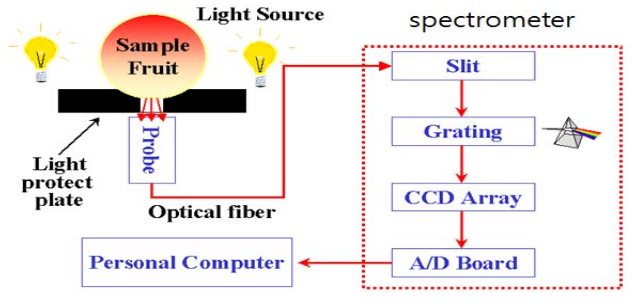
\includegraphics[width=0.7\linewidth]{spectroscope.png}
	\caption{Example of a spectroscope taking measurements from a fruit sample.}
	\label{fig:spectroscope}
\end{figure}%


Matteoli et al \cite{matteoli} used a fibre-optic spectrometer to take measurements of peach fruits whilst performing destructive density testing in order to make predictions on new fruit non-destructively. They compared the output of a crisp versus fuzzy logic approach and found overall average accuracies of $60\%$ and $~80\%$, respectively, making the fuzzy system appropriate for the task. Choi et al \cite{choi} also used an NIR spectrometer to assess the internal qualities of pear fruit as well as CCD cameras to inspect the visible characteristics such as skin blemishes and colour. The spectroscope analysed the fruit for sweetness, acidity, hardness, and moisture before combining the two (visible and internal) features as variables for an ANN, achieving a classification accuracy $97.4\%$.

A hyperspectral range of $400nm-1000nm$ was used by ElMasry et al \cite{elmasry2} to inspect various fruit by it's moisture content (MC), soluble solids (TSS), and acidity(pH). The resulting correlation coefficients of both the Partial Least Squares ($0.90, 0.80, 0.87$, respectively) and Multiple Linear Regression ($0.87, 0.80, 0.92$, respectively) proved the feasibility of predicting these physical characteristics. They also measured three ripeness classes based on grey-level co-occurrence matrix (GLCM) analysis achieving $89.61\%$ classification accuracy.


Beyond the Near (NIR), Short (SWIR), lies the Mid (MWIR) Wavelength Infrared, and  Long Wavelength infrared (LWIR) which is the part of the spectrum ($3\mu m-15\mu m$) in which objects near room temperature emit thermal radiation. This thermal information can be detected by specialised sensors and converted to correlated visible colours for humans to view as seen in Figure \ref{fig:thermal} taken from \cite{baranowski}.

\begin{figure}[h]
	\centering
	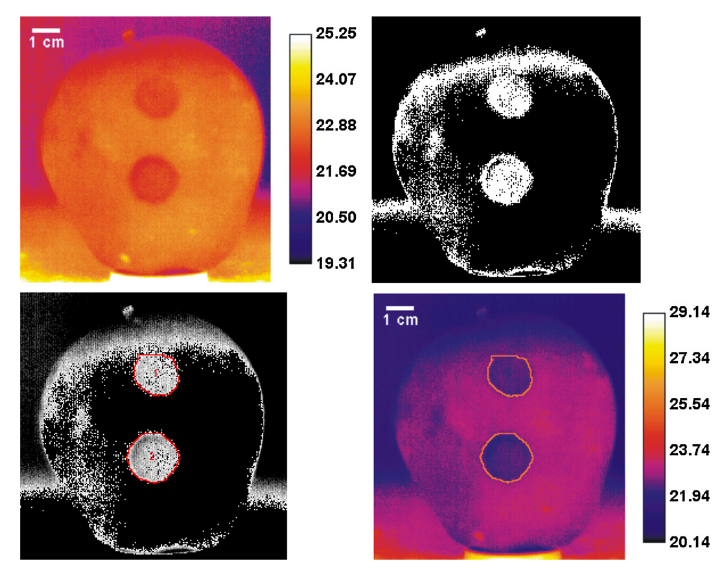
\includegraphics[width=0.8\linewidth]{thermal.jpg}
	\caption{A thermal image apple with bruises showing the Long Wavelength Infrared (LWIR) part of the electromagnetic spectrum. In this range, sensors can detect thermal properties at room temperature}
	\label{fig:thermal}
\end{figure}%


Thermographic images in the wavelength range $3.4-5.2\mu m$ assisted Ginesu et al \cite{ginesu} to develop a thermal inspection system used to detect foreign bodies in produce items on a production line. Thermal imaging requires heating or cooling in order to stimulate the subjects before being imaged sometime afterwards. Different material's heat transfer rates are varying, making the process of distinguishing, for example, sticks or stones from the edible items. They used a contrast enhancement and region-growing method to extract the highlighted regions from the greyscale thermal images.

On the opposite side of the visible spectrum resides ultraviolet, followed by X-ray wavelengths at which common medical and security inspections occur. X-rays are capable of penetrating objects in, for example, airport security allowing the users to visually inspect the contents of luggage. Medical applications include bone tissue and organ imaging in order to help physicians make informed decisions about patients. By choosing the optimal wavelength, many materials can be visualised internally including fruits and vegetables.    

Mathanker et al \cite{mathanker} analysed good and defective pecans using X-ray images. They compared AdaBooost and SVM classifiers finding that the AdaBoost average classification result of $92.2\%$ was the best performing. Cost, precision and speed of X-ray sensors and equipment has made food inspection problems unfeasible in the past, however as technology improves over time, adoption of these systems increases cost-benefit margin and is more attractive to producers \cite{haff}.

A laser backscattering technique used by Lorente et al \cite{lorente} provided images that could determine the presence of pathogen Penicillium digitatum in oranges. They directed a laser beam onto the fruit and took images of the surface reflectance using five laser wavelengths ($532nm$, $660nm$, $785nm$, $830nm$, and $1060nm$) in order to perform experiments differentiating sound and decaying flesh with the best average accuracy results of $96.1\%$ attained by using all 5 wavelengths in combination trained with an LDA classifier. The single wavelength, and two-wavelength average accuracy scores were $80.4\%$ and $90.2\%$, respectively.



\section{Hyperspectral/Multispectral Imaging}
\label{sec:lit_hyperspec}

As the spectral range of the eye is limited, camera sensors can be employed which can visualise wavelengths beyond these restrictions into the ultra-violet and infrared ranges. Figure\ref{fig:eye_sensor} shows the spectral response of the human eye versus CMOS and CCD sensors illustrating the extent to which the electronic sensor's range is greater.

\begin{figure}[h]
	\centering
	\begin{subfigure}{.9\textwidth}
		\centering
		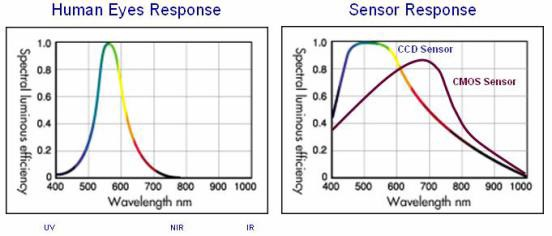
\includegraphics[width=0.9\linewidth]{spectralresponse.jpg}
		\caption{}
		\label{fig:eye_sensor}
	\end{subfigure}

	\begin{subfigure}{.9\textwidth}
		\centering
		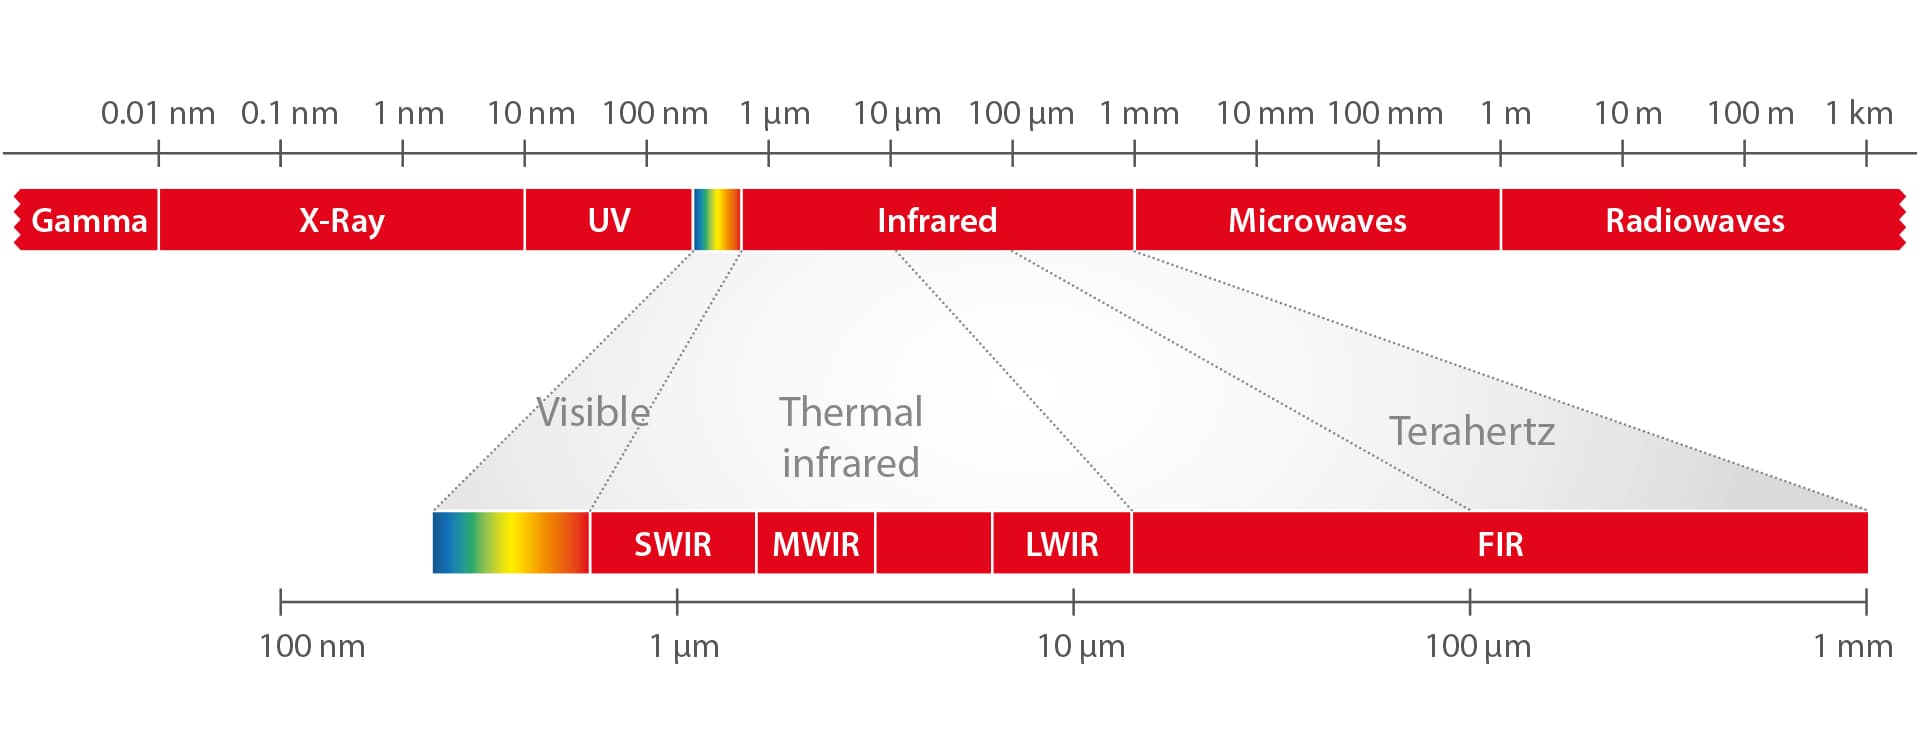
\includegraphics[width=.9\linewidth]{infra-red.jpg}
		\caption{}
		\label{fig:ifra-red}
	\end{subfigure}%
	\caption{(a) Spectral response of human eye (left) and CCD and CMOS sensors (right). (b) Infrared}
	\label{fig:spectrum}
\end{figure}%

Other sensors exist whose range is further into the infrared (SWIR, MWIR, LWIR, and FIR in Figure \ref{fig:ifra-red}), allowing many properties (usually internal) to be analysed.

Classification can be performed using hyperspectral imaging as well as defect detection. Invisible properties of fruits and vegetables in particular, can be used to classify between species, or grades of a particular species. Munera et al \cite{munera} developed a system using visible and NIR hyperspectral imaging in order to grade persimmon fruit by firmness, maturity level, and astringency. Using CIE-Lab colour space, they found that the $L$ and $b$ coordinates decreased whilst the $a$ coordinate increased with maturity, allowing good correlation with colour parameters such as $H(R^2 = 0.83)$, $G(R^2 = 0.82)$ and $h(R^2 = 0.81)$. Ratios of the colour channels were also analysed with results achieving $a/b(R^2 = 0.83)$, $G/R(R^2 = 0.83)$, and $a/L(R^2 = 0.83)$. Three wavelengths were chosen as optimal ($580nm$, $680nm$, and $1050nm$) in order to perform the ripeness tests with all accuracy $>94\%$ using LDA, QDA, and SVM classifiers. The astringency test used the same classifiers and resulted in $>90\%$ for all, and $>95\%$ for the QDA method. This indicates the ability of non-destructive assessment of the maturity, firmness, and astringency of these fruits is valid. Another example by Munera et al \cite{munera2} acquired images with wavelengths of $450nm-1040nm$ for the purpose of distinguishing between two kinds of nectarine that have very similar appearance but different taste. A human panel could only classify correctly $57\%$ of the time, whereas their method had a $94\%$ accuracy using a PLS-DA model trained with 14 optimal wavelengths. 

In order to grade cherries into three maturity stages, Li et al \cite{li} analysed characteristics in terms of Soluble Solids Content (SSC) and acidity (pH) with hyperspectral imaging in the range of $874nm-1734nm$. Two full-band methods were tested, namely, principal components regression model and partial least squares regression model both with similar accuracy. A genetic algorithm (GA) was used to reduce complexity in bandwidth by reducing the full spectrum to 54 optimal bands for the SSC model and 28 for pH, and reported a $96.4\%$ total accuracy.  


Bruising in soft-skinned fruit and vegetables occurs if mishandled or exposed to excessive handling, reducing the quality for customers. Usually resulting from an impact, the moisture comes to the surface and therefore can be differentiated from the surrounding sound tissue by means of analysing several water absorption bands in the visible and NIR regions. Therefore, NIR and SWIR wavelengths can penetrate the surface of some materials giving insight into hidden or skin defects ranging from sub-surface bruising to external visible tissue damage. Visualising these impurities can be challenging for RGB imaging given inerrant colour saturation and reliance on good illumination. 

Using hyperspectral imaging ranging from $950nm$ to $1650nm$, Lee et al \cite{lee} exploited the ability of NIR wavelengths to detect bruising in pears. By investigation it was found that the waveband ratio of $1074nm/1016nm$ highlighted invisible bruises which could then be extracted using thresholding with a $92\%$ accuracy. 

Hyperspectral imaging and PCA reduction used by Che et al \cite{che} provided an accurate method to extract bruise regions from apple images. Using two characteristic wavebands at $675nm$ and $960 nm$, they analysed the fruit $0h$, $12h$, and $18h$ after bruising impact and found that the Random Forrest classifier performed best at $99.9\%$ average accuracy. Qiang and Mingjie \cite{qiang} used hyperspectral imaging  in the range of $408nm-1117nm$ in order to detect bruising in kiwi fruit. They were able to detect the bruising through the thick peel where human vision could not with an overall error rate of $14.5\%$. Li \cite{li3} also investigated detection of bruising on peaches in the invisible NIR and SWIR range only ($781nm-2500nm$) in combination with and improved watershed segmentation technique resulting in a bruise detection accuracy of $96.5\%$ and sound sample detection accuracy of $97.5\%$.

Other species have similar bruise detection properties with infrared imaging such as apples \cite{che}, kiwi \cite{qiang}, and Pear \cite{lee}. Lopez-Maestresalas et al \cite{ainara} investigated two wavelength bands at Vis-NIR ($400nm-1000nm$), and SWIR ($1000nm-2500nm$)in order to detect black-spot in potatos which occurs on heavy impact during harvesting. The dark skin of the potatos inhibits visual detection for black-spot going largely undetected. Their analysis showed that, using HSI colour space and PLS-DA, they could achieve an overall classification accuracy of $>94\%$. This result was superior over the other methods examined, namely, PCA and Soft Independent Modelling of Class Analogy (SIMCA). They also found that the SWIR band possessed features which allowed early detection of the defect with $98.56\%$ accuracy $5h$ after impact.

A strawberry decay detection method designed by Liu et al \cite{liu2} used SWIR ($1000nm-2500nm$) imaging to determine attributes such as Total Water-soluble Sugar (TWSS), the sum of fructose, glucose, and sucrose finding several distinct bands to evaluate. Predicting the TWSS content resulted in $R^2=0.807$ correlation coefficient and the accuracy of the decay classifier generated between $89.4\%-95.4\%$ for calibration and $87.0\%-94.4\%$ for prediction accuracies, respectively.

Skin defects in bi-coloured peaches were successfully detected by Li et al \cite{li2} by investigating wavelengths from $400nm$ to $1000nm$ determining characteristic values at $463nm$, $555nm$, $687nm$, $712nm$, $813nm$, and $970nm$ as well as $781nm$, $815nm$, and $848nm$. The best results of $96.6\%$ were realised when taking the ratio of $781nm/848nm$.

Strawberry fungal infection identification performed by Siedliska et al \cite{siedliska} analysed wavelengths in the range of $400nm-2400nm$ finally selecting 19 bands to discriminate infected vs sound berries training a BNN model. They achieved $>97\%$ accuracy for discriminating between infected and control fruit from the $24h$ point, and using the same bands, performed a multiple linear regression technique to predict anthocyanin content (AC) and soluble solid content (SSC) with results of $R^2=0.65$, and $R^2=0.85$ coefficients, respectively.





\section{Strawberry Vision Systems}

Strawberries are a delicate fruit with an unprotected, soft, edible flesh, and very susceptible to damage if mistreated, handled too much, or even transported carelessly. The outer flesh of the berry is cratered with seeds generating higher surface friction, as well as an incredibly soft exterior, creating challenges in terms of handling practices during picking, packing, and distribution. This is not the case for fruits such as mango, watermelon, oranges, kiwi, and banana, for example, which have a protective, smooth layer of peel to protect the flesh inside, seen only by the consumer. Some success has been made in machine vision for strawberries, with examples in robotic picking, picking and grading, and grading on a production line. 

Brosnan and Sun \cite{brosnan} performed a review of agricultural vision systems including apple grading, orange stem detection and sweetness correlation, defective pistachio nuts, tomato size, colour, and shape properties as well as seedling health, peach and pear maturity levels, and automatic fruit harvesting. The team also reviewed vegetable inspection methods such as mushrooms and potatos, as well as wheat, rice and corn. They described 2 methods for analysing strawberry shape and size, taking one of the teams $1.18$ seconds per berry to analyse only shape and size, noting that fruit quality is dependant on a number of pre-harvest and post-harvest processes. The hardware used was a Pentium\textregistered $200MHz$ processor and a Sony\textregistered CCD-IRIS/RGB camera, indicating a potential to reduce this processing time by greater than a factor of 10 ($2GHz$) in modern computers.

Using a conveyor system, L. Xu et al \cite{xu} achieved very good results in classifying shape, ripeness, and size. The measurements are attained by using a K-means clustering method to find 7 vertical and 7 horizontal axis lines. Size feature was calculated by performing experiments to find the ratio of pixels/mm and simply dividing the pixel measurements of the berry by this ratio. Using the CIE-Lab colour space, a dominant colour was found in the berry by means of a histogram windowing method. Similarly, Liming and Yanchao \cite{liming} developed a strawberry grading method and mechanical system that requires manual loading of single strawberries on a conveyor belt before using colour features and k-means clustering to grade the fruit into shape and colour classes at a rate of approximately $2.5s/berry$. An Advantech\texttrademark PCM9575 all-in-one $800Mhz$ computer was used to process images from a Panasonic\texttrademark WV-CP470 with resolution of $525x480$. 


\begin{figure}[h]
	\centering
	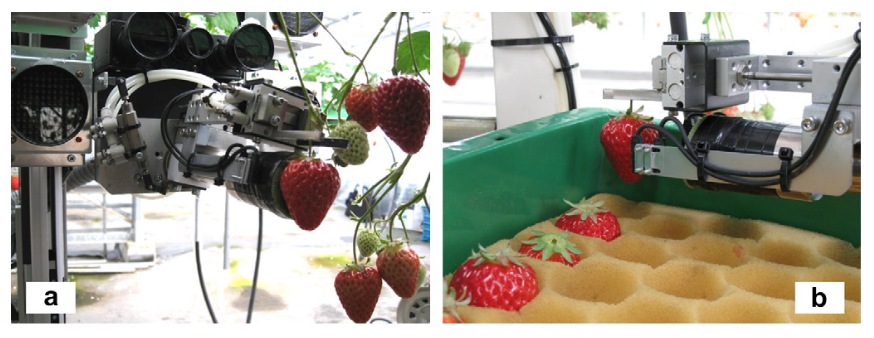
\includegraphics[width=0.9\linewidth]{strawberry_picker.png}
	\caption{Strawberry picking machine (a) demonstrating end-effector mechanism (b) placing strawberry into the foam tray.}
	\label{fig:strawberry_picker}
\end{figure}%


S. Yamamoto et al \cite{yamamoto2} used simple RGB techniques to define the ripeness of strawberries when developing an automated harvesting machine. They used a combination of green, red, and white LED's in order to illuminate the strawberries in specific wavelengths, giving better judgement on whether to pick or not based on ripeness. The harvesting machine was designed to be stationary with the fruit being presented to the machine via moving beds, which implies a large amount of fabrication and process change would be required to pursue this method. The authors reported high harvesting rates ($67.1\%$) compared to that of other more conventional harvesters, however, their system was susceptible to fruit damage and requires improvement in harvesting speed. Hayashi et al \cite{hayashi} reported a rate of $11.5s/berry$ using their automated harvesting machine. The end-effector designed by the team used a peduncle cutter in conjunction with a suction cup to pick the fruit from the plant and place it in a padded tray as shown in Figure \ref{fig:strawberry_picker}. The HSI colour space was used to generate a maturity level when grading the fruit to be picked. By creating acceptable and unacceptable sections of the average hue, saturation, and intensity channels, they could discern $>80\%$ ripeness with an accuracy of $41.3\%$.


Strawberries are farmed with a range of different cultivar and seasonal characteristics making their distinguishing features seem obvious only to expert humans. This is shown by Yamamoto et al \cite{yamamoto} when they implemented a method to distinguish between 21 different strawberry cultivars. They found that when using a single feature such as colour, shape, or size, the average accuracy was very poor at $<42\%$. However, when these three features were used in conjunction, the discriminant analysis classifier performed better at $68\%$. This shows that strawberry cultivars are not simply classified as the inter-species colour and form can possess similar features. 


\begin{figure}[h]
	\centering
	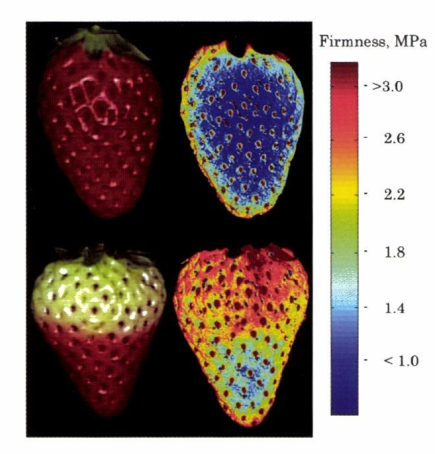
\includegraphics[width=0.5\linewidth]{multispec_strawberry.png}
	\caption{Pseudo-coloured strawberry heat-map showing the white area of the berry being firmest and the red area softest.}
	\label{fig:multispec_strawberry}
\end{figure}%

EMasry et al \cite{elmasry2} used multi-spectral imaging in order to determine the moisture, soluble solids, and pH levels in order to grade the ripeness of single strawberries. They found broadband absorption bands, in the case of under ripe fruit, at 500, 680, 840, and $960nm$. The bands at 840 and $960nm$ were found to represent sugar and water absorption which was used to determine factors that would usually require destructive testing. The same results were found by Tallada, Nagata, and Kobayashi \cite{tallada} using an NIR hyperspectral system, they analysed and assessed the firmness of strawberries by non-destructive imaging. By taking acquiring images from $640nm-1000nm$ in steps of $5nm$ they were able to determine the optimal wavelengths to estimate firmness across three grades of ripeness. The results had a correlation coefficient of $R^2=0.786$ and standard error of $0.350MPa$ using $685nm$, $865nm$, and $985nm$. They calculated formula to generate heat maps of the firmness distribution (pseudo-colour), as shown on the ripe and under ripe examples in Figure \ref{fig:multispec_strawberry}. This result is expected given the deep red colour of the top specimen versus the half white, and red example.

Zhang et al \cite{zhang} used a hyperspectral imaging system in two ranges - $441nm-1013nm$ and $941nm-1578nm$ to assess the ripeness of strawberries into three categories. Using PCA for reflectance processing and texture components at optimal wavelengths to form the feature set, they trained an SVM classifier achieving overall classification accuracy of $85\%$. Similar research by Liu et al \cite{liu} used 19 bands in the range of $405nm-970nm$ in order to determine firmness, SSC, and ripeness. Experimenting with classifiers such as SVM and PLS, they found the BPNN model performed well with $R^2=0.94$ and $R^2=0.83$ coefficient of prediction for firmness and SSC, respectively. Three category ripeness evaluations were performed using both PCA-BPNN and SVM classifiers with the SVM model achieving $100\%$.

 




\section{Real-time Systems}

One important aspect of developing vision systems designed for quality inspection is the process of production implementation. Accuracy, speed, safety, power, robust design, operator use, control mechanisms, and signals must all be considered in order to progress from bench design to production-ready. Control mechanisms and speed of processing are the most prominent of these considerations, with many solutions using simplified processes.

Fruit and vegetables are generally graded by the ripeness or readiness to eat, based in predominance on their colour, size, and texture. Therefore many solutions to real-time grading use simple colour algorithms, many in combination with size and texture estimation. Sofu et al \cite{sofu} designed the automatic apple sorting system described in Figure \ref{fig:apple_system}, processing at a rate of $54,000 apples/h$ achieving an accuracy of $79\%$ using a simple decision tree to classify the specimens according to colour, size, stain and weight before sorting the apples using opening bowl mechanisms. This demonstrates the components of a real world production-operated inspection unit including safety systems, user interface, user control panel, product control system, lighting enclosure to reduce noise, and multiple cameras acquiring images at high speed. Each of these features will need to be implemented to any production system in order to be safe, effective, and accurate.

\begin{figure}[h]
	\centering
	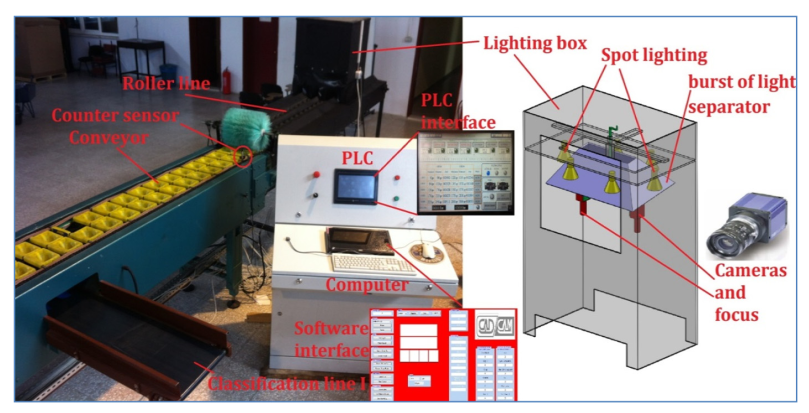
\includegraphics[width=0.7\linewidth]{apple_system.png}
	\caption{Apple sorting system showing the lighting box with cameras in the background with opening bowls in the foreground.}
	\label{fig:apple_system}
\end{figure}%

A fig sorting system developed by Baigvand et al \cite{baigvand} could successfully categorise the figs into five grades with accuracies up to $95.2\%$, processing at a rate of $90kg/h$ and sorting each into separate bins using air nozzles. The team created indices related to colour, size, and the area of the split, seen on each fruit, applying a rule-based method to determine the graded category. Many real-time sorting systems exist, for example, Duan et al \cite{duan} used a system of two cameras and two computers to inspect glass beer bottles after production at a rate of $500/min$ or $8.3/s$. They inspected the bottom of the bottle, the overall finish, and the top opening, performing all three checks for each bottle within the time frame specified. After inspection, the defected bottles are ejected from the production line in order to be recycled. Elmasry et al \cite{elmasry1} developed a potato grading system which can acquire multiple images of each potato, from multiple sides due to the roller-conveyor, before performing Fourier transform, and Fourier shape descriptors. The conveyor speed is $1m/s$ and the spacing between each roller is $80mm$ giving approximately $12 potatos/s$ if there are no empty rollers. Four different grading/processing techniques were investigated by Kondo \cite{kondo} where, firstly, oranges were inspected by a system of cameras including six colour cameras at different positions (so that all sides are inspected), an NIR camera and the option of adding x-ray imaging to the purpose-built line. The oranges are fed through the system using a singulating conveyor which performs a $180^{\circ}$ rotation for the last camera to ensure all sides are evaluated. Secondly, an eggplant quality assessment system was developed which made use of six colour and four monochrome cameras in order to determine colour, size, shape, and defects as well as a novel gloss detection method using angles cameras and three white strip lights to inspect the specular reflections sharp edges, meaning good quality, or dull edges, meaning poor. The 6 production lines, running at $38.1m/min$, at the facility meant that $504,000$ fruits could be processed per day. Even though there has been a substantial reduction in number of employees in processing, it is still laborious due to the packing requirements. The third project was capable of grading $10,000$ leeks per hour at a line speed of $30m/min$ with automatic root cutting and peeling steps. Lastly, a robot capable of grading $3 fruit/sec$ for 11 varieties of deciduous fruits including apple, pear, and peach. Using 3 DOF manipulators, the robot placed into trays, whilst images are acquired from top, bottom and two sides before making a grade decision. 


In order to remove the green calyx from strawberries, Lin et al \cite{lin} used a water jet cutting system guided by machine vision. The strawberries were fed into the system using roller rods to align and separate before using CIE-Lab colour space to segment the berries from the calyx. A series of geometric calculations guide the cutting system with the optimal cut line. Their machine was designed to process berries bound for ice cream, yoghurt, juicing, and jam markets instead of being packaged for sale as fruit, meaning that condition, bruising and ripeness was not of concern as much as removing the green leaves.

Hyperspectral and multispectral implementations can help systems to assess products in real time due to their ability to detect what the human eye, or regular cameras cannot. This advantage can provide information which simplifies the processing of images, for example, the use of NIR wavelengths can uncover invisible defects (as discussed in Section \ref{sec:lit_hyperspec}). Lee et al \cite{lee} implemented an industrial date grading machine capable of processing $72,000 dates/h$ with an $87\%$ accuracy measured. They acquired images in NIR wavelengths ranging $750-1200nm$ by use of an NIR-extended CCD camera and a high pass filter to block wavelengths lower than $750nm$. Processing at a rate of $20 fruit/s$ ,these wavelengths provided good background segmentation, added to the amplification of delaminated skin features which determine quality. The amount of delaminated skin was calculated, after morphological operations, and compared to the size of the entire fruit to give a percentage and a grade from 'A' to 'E'. 

When implementing systems in production environments, the rate of production (and limited space constraints) sometimes require inventive solutions to be implemented in order to achieve the desired outcomes. Aleixos et al \cite{aleixos} developed a commercial citrus grading system which used a combination of transmissive and reflective lenses in order to image the same scene with two cameras. One RGB and one NIR camera were used to acquire images of citrus fruits at a rate of $5 fruits/s$ before assessing each for size and colour and surface defects. The size estimation had $<2mm$ error with colour grading for oranges, lemons, and mandarins reaching $94\%$, $93\%$, and $94\%$, respectively.

Machine vision can outperform humans depending on the task involved. Particularly for borderline cases a machine has finite thresholds in place to ensure consistent outcomes. Estimating ripeness colour, areas of scattered blemishes, and measurements can be difficult and/or subjective between human experts but easily calculated with vision systems. A meat marbling grading system developed by Barbon et al \cite{barbon} trained a k-NN classifier to grade meat samples in $<1s$, which is an improvement on human gradation time of $11s$. Their method was suitable for a range of lighting conditions and animal type due to the illumination normalisation and contrast enhancement processes before classification attaining results of $81.59\%$ and $76.14\%$ for bovine and swine, respectively. 



\section{Machine Learning / Deep Learning Methods}


Machine learning is a branch of computer science and AI that uses an iterative 'learning' approach to building a classifier model. The model's weights are updated by an algorithm that, given any training set ($x_1, y_1$), ($x_2, y_2$), ... , ($x_n, y_n$), can learn a function $y = f(x)$ to make prediction of an unseen $x_{test}$ variable. Deep learning refers to the depth of the network or number of layers the model has. Using a deeper network allows for multiple convolutions in a CNN and therefore better abstraction, albeit more computationally expensive. A range of methods have been investigated from very basic MLP networks, SVM, and ANN to more complex architectures such as CNNs.


Comparison of MLP neural network and Discriminant Analysis (DA) performed when grading golden delicious star fruit by Abdullah et al \cite{abdullah} found that the colour attributes were more accurately classified by DA, with resulting $95.3\%$ and $90.5\%$ for DA and MLP, respectively. The method used to extract colour features based on hue values $10-74$ were improved with the DA classifier using Wilks-lambda reduction, however the MLP result was unchanged. In order to classify shape characteristics, Fourier descriptors were used generating a $100\%$ accuracy.


Zhang et al \cite{zhang} used an FNN to classify a fruit dataset created via on-site collection and on line. After background removal, the 79 features that had been constructed based on colour, texture, and shape were obtained before being reduced via PCA to 14, and used to train the network using 5-fold cross validation. The classification accuracy of $89.1\%$ outperformed other methods tested such as BP, momentum BP, and GA. 

Even for simple networks, the relationship of problem domain to network architecture is not well defined in terms of accuracy. Zuniga et al \cite{zuniga} used a supervised learning approach with small ANNs in order to grade grape seeds from images acquired scattered over a flat-bed scanner. Using a process of analysis and trial and error, the optimal number of neurons is found and a classifier trained giving total accuracy of $86\%$ for the test set. An apple grading system developed by Vakilian and Massah \cite{vakilian} used a 3-layer ANN whilst grading Golden Delicious and Red Delicious varieties with respective overall accuracies of $89\%$ and $92\%$. Extracting the images textural (mean and variance of energy values) features before training separate networks for each apple variant. Finally, they instigated the width of the ANN's middle layer ranging the architecture of the network from $2-2-4$ to $2-20-4$ finding the optimum width of $2-12-4$. 

Conversely, Wang et al \cite{wang} had perfect results using a similar architecture whilst developing a method to find worm-eaten holes in chestnuts. Using Sobel edge detection and using the resulting, filtered region to train a BP network. Conversion occurred after only three iterations and achieved $100\%$ for both good and wormhole classes.

When using hyperspectral/multi-spectral data, it is possible to extract internal attributes such as structure, soluble solids (sugar content) and pH levels depending on the subject and wavelength range. Sugiyama et al \cite{sugiyama} were able to detect stems and leaves (foreign objects) from hyperspectral blueberry images. They found that the foliage was easily extracted at particular wavelengths (1268 and $1317nm$) and were then able to perform a discriminant analysis between the two wavelengths in order to segment and highlight the defects.

An ELM is used to train a single hide layer feed neural network (SLFN) in a more efficient way by performing a random feature mapping and a least squared formula based linear regression \cite{peng}. Luo et al \cite{luo} used a kernel extreme learning machine to create a multi-label classifier used in applications where designators are applied to an unseen object. Xu et al \cite{xu} used an ELM to continuously modify it's classifier in a dynamic process due to concept drift in applications. Extra nodes are added when an alert flag is set in the algorithm, and if the error rate drifts too far, the classifier is erased and a new classifier is trained. A novel twin ELM algorithm was used by Wan et al \cite{wan} to train two classifiers simultaneously by creating two non-parallel hyperplanes. 

ELM have proven to be an efficient and accurate method to train classifiers due to the least square formulation approach to find the solution, opposed to the first and second order gradient descent method \cite{yavs}. the ELM out-performs other classifiers such as SVM and k-NN which have been tested independently \cite{yavs, wan, peng}, due it's combination of fast training times, testing times, high accuracy, and low error rate. Several applications were able to implement ELM in real time systems due to these factors \cite{xu, yavs}.  

Mohammed et al \cite{mohammed} used a novel Bi-directional two Dimensional Principal Component Analysis (B2DPCA) in conjunction with an Extreme Learning Machine (ELM) in order to greatly improve facial recognition accuracy in popular face datasets. The B2DPCA technique proposed keeps the data in matrix form as opposed to vector form for PCA processing, and the ELM is a variation of a feed forward, single hidden layer neural network, with the main difference being assignment of random input weighs and hidden layer biases which transforms training the network into a linear system. Zheng, Fu, and Ying \cite{zheng} used an Extreme Learning Machine (ELM) to classify spectroscopic data acquired from four different foods - coffee, meat, oil ,and fruit. The results indicate good results for the coffee, meat, and oil with $100\%$, $97.78\%$, and $97.35\%$ accuracy, respectively, whilst the fruit classification was less accurate achieving $95.05\%$. They compared all the datasets and ELM by applying five different methods including KNN, DA, and ANN, finding that SVM was the most appropriate. 


\subsection{Support Vector Machines}


SVM can be considered a type of neural network that has only one hidden layer of neurons. The SVM attempts to create a hyperplane between the feature sets of each class (Figure \ref{fig:SVM}). The support vectors are formed as non-zero coefficients of the data points found after processing the training set. If the margin is large between the hyperplane and each class, the system is said to be a stronger SVM classifier and should produce good results as explained by Osuna, Freund, and Girosi \cite{osuna}. Standard SVM inherently is incompatible with large datasets which suits applications with a small set of training examples. This is due to the $O(m^3)$ training time and $O(m^2)$ space complexity where $m$ is the size of the dataset \cite{tsang}.


\begin{figure}[h]
	\centering
	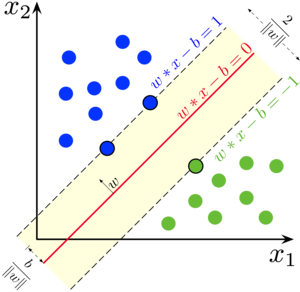
\includegraphics[width=0.5\linewidth]{SVM.png}
	\caption{A 2D example of SVM hyperplane separating two classes. The examples on the boundary are considered the support vectors.}
	\label{fig:SVM}
\end{figure}%

Given a set of training data {$(x_i, y_i), x_i \in X^n, y_i \in (-1,1), i = 1,2,3,...,n$} the SVM kernel attempts to solve the hyperplane decision boundary equation:
\begin{equation}
w \cdot x + b = 0
\end{equation} 
giving
\begin{equation}
w \cdot x + b \geq 0, \quad \textrm{for} \quad y_i = +1
\end{equation}
and
\begin{equation}
w \cdot x + b < 0, \quad \textrm{for} \quad y_i = -1
\end{equation}

Here, $w$ constitutes the weight vector, $x$ the variable vector, and $b$ the bias scalar. Beginning with the kernel function $K(x, x^\prime)$ which obtains the non-linear mapping $\Phi(x)$, the solution takes the form:
\begin{equation}
f(x) = b + \sum_{i=1}^{m} y_i \alpha_i K(x, x^\prime)
\end{equation}
which is the summation of each support vector of length $m$, the respective $y$ values, Lagrangian multiplier ($\alpha_i$), and the kernel $K(x, x^\prime)$.


An SVM classier trained by Sabri et al \cite{sabri} was able to classify ripe and unripe palm oil fruits with an accuracy of $96.59\%$. They compared three methods of feature extraction (Colour histogram, colour moment, and colour correllogram) and two classification methods (SVM and Naive Bayes) in order to find the best results with SVM prevailing. Chen et al \cite{chen} performed an SVM parameter search to find the best combination whilst colour grading beef fat. They segmented the fat by use of boundary tracking, thresholding, and morphology achieving $97.4\%$ classification accuracy. Mizushima and Lu \cite{mizushima} used SVM to generate greyscale images that increased the contrast of Golden Delicious apples for segmentation purposes, before again using SVM to classify them into three grades reporting $1.42\%$ error across all three classes. They also achieved fast processing speeds of $1.5ms$ using a $3.4 GHz$ CPU showing that SVM is capable of very fast and accurate predictions. 

However, SVM was not the predominant classifier when Alfatini et al \cite{alfatni} designed a palm oil grading application. The method consisted of using a basic grey level aura matrix (BGLAM) technique to extract features followed by an ANN classifier. After assessing ANN, KNN, and SVM classifiers, the best results were realised using the ANN with accuracy of $93\%$ and speed of $0.4s$. An ANN was also used by Bhatt and Pant \cite{bhatt} opposed to SVM, when grading apples based on size, colour, and external defects. Seven selected features were used (3 colour features, 1 size, 1 damage, 1 symmetry, and 1 weight) to train the ANN achieving $90\%$ testing accuracy. 



\subsection{Deep Learning}

Machine learning is a broad term that encapsulates Artificial Intelligence (AI) techniques adopted from many approaches, and can be defined as any  computer program that can perform tasks, after having been trained,  without having to be explicitly told to \cite{langley,shavlik,mohri}. In other words, the program can adapt and configure itself to specific conditions in order to make decisions, improve accuracy or efficiency, control systems, and predict outcomes among many other uses. The \textit{learning} is a term that refers to the process of training a program to perform a task. Given a training set $(x_i, y_i)$, $x\in X$, $y\in Y$ of inputs and outputs, the program must derive a function $f$ that satisfies $f(x_i) = y_i$ for all $i$. A very large training set will improve accuracy, however, this may result in extremely long periods of training (weeks in some cases \cite{bottou}), or over-fitting problems. Training can be sped up, however, by increasing computational power such as high-end GPU's or supercomputer systems.

Neural Networks are a commonly implemented method in order to perform many functions and are made up of one or more layers of neurons as shown in Figure \ref{fig:neural_net}. The layers in this image are fully connected, meaning that each neuron in the layer $L_n$ takes inputs from the layer at $L_{n-1}$, and can output to the layer at $L_{n+1}$, however, neurons in the same layer may not be connected. This is the most common approach, although, sometimes it is beneficial to avoid fully connected layers. An SVM classifier can be thought to be modelled as a single layer NN, and other terms have evolved such as Artificial Neural Networks (ANN) and Multi-layer Perceptron (MLP). However, more complex topologies can be constructed with the addition of convolutional steps between layers, known as a Convolutional Neural Network (CNN) and the term deep learning or Deep Neural Networks (DNN) where the depth is seen in the number of connected layers.  


A neural network sums the weights and biases at each neuron in each layer mathematically represented by: 
\begin{equation}
a_i = f\bigg\{b + \sum_{i=0}^{n} w_i x_i \bigg\}	
\end{equation}
After computing these neuron activations, the Back-Propagation (BP) process is used in order to update the weights and bias. This is done by firstly assessing the cost of the output of the network versus the training sample value ($y_i$). The cost $C_{w,b}$, where $w$ is all weights within the network, and $b$ the bias, is given by:
\begin{equation}
C_{w,b} = \frac{1}{2n} \sum_{i=0}^{n} \|y_i - a\|^2	
\end{equation}
This cost function is minimised (training process) by using methods such as gradient decent to arrive at the optimal solution, where the small change in cost $C$ takes the form:
\begin{equation}
\Delta C \approx \frac{\partial C}{\partial w} \Delta w + \frac{\partial C}{\partial b} \Delta b	
\end{equation}

These parameters are calculated and updated at each pass (epoch) and therefore may be set to some value initially, but may only be changed by the computations thereafter. Figure \ref{fig:conv3} shows an example of a convolutional network (ConvNet) with the two prominent intermediate steps of convolution and pooling/subsampling in the feature extraction section. For deep learning algorithms in image analysis, the matrices are proportional to the resolution of the image and hence can be manipulated using computational programming languages. 

Convolution is the process of 'windowing' a set of feature masks over an image (or feature set in the form of a matrix) and taking the resulting calculations as the new feature set. This results in a smaller yet more salient feature set spatially, while the dimension (channels) increase with number of masks. Each feature mask or filter (which may be as small as 3 x 3 pixels) has the same weights for each filter convolution, greatly reducing the number of biases and weights (since they are the same for each convolution at that layer). 

\begin{figure}[h]
	\centering
	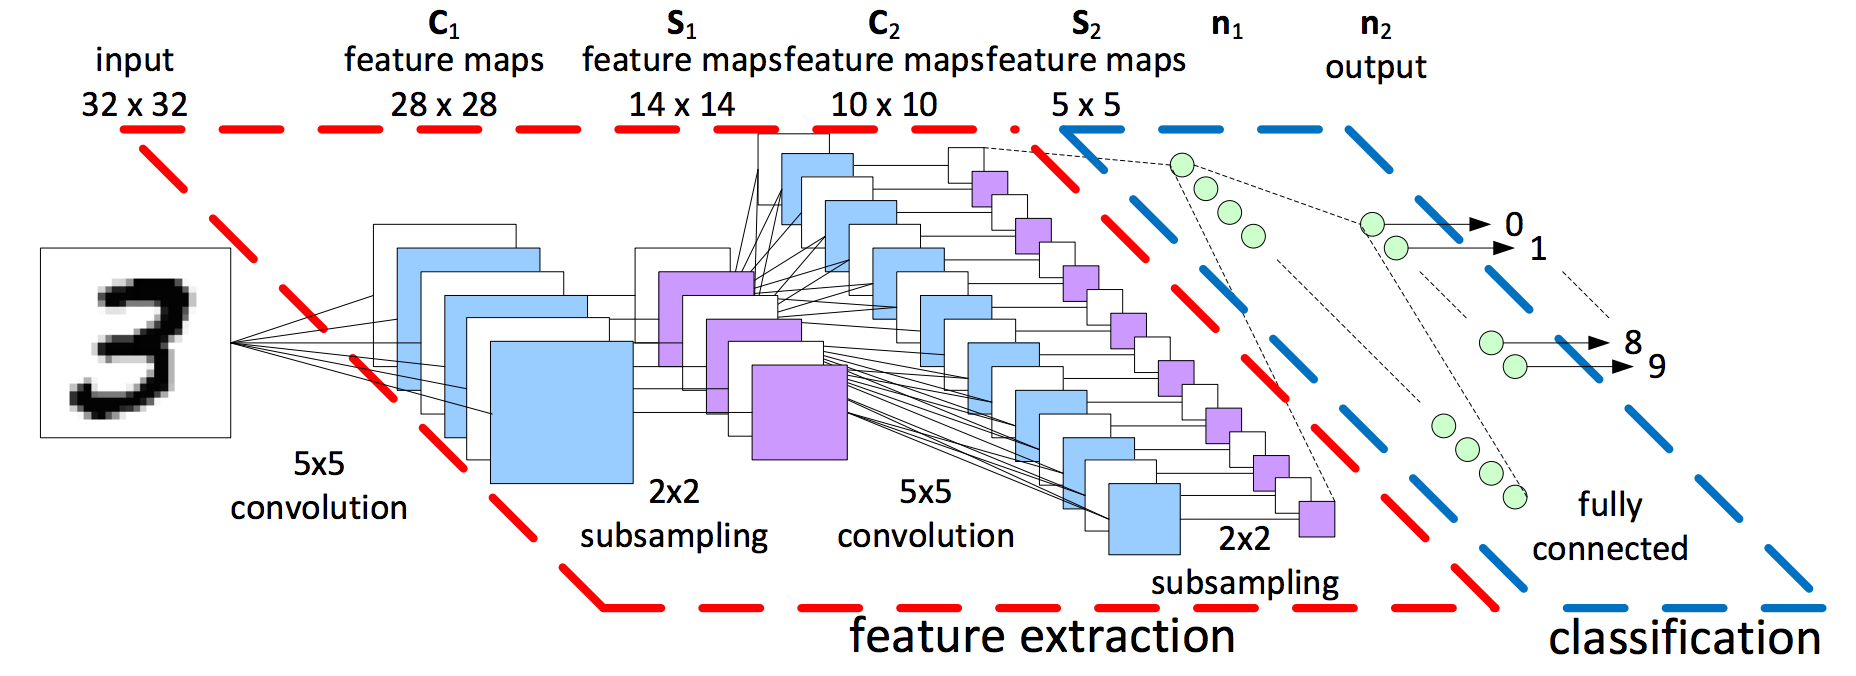
\includegraphics[width=\textwidth]{conv3.png}
	\caption{An example of a ConvNet pass showing convolutional layers, subsampling (pooling), and finally, fully connected layers in the classification section.}
	\label{fig:conv3}
\end{figure}

The convolution occurs relative to the number of pixels/steps per window movement, or stride. The output, will therefore compute a 2D feature map where the size is dependent on stride and feature map size, and depth of feature maps are equal to the number of feature masks used. In the example in Figure \ref{fig:conv3} uses six filters to transform the input image from 32 x 32 x 1 image into 28 x 28 x 6, with multiple Conv layers finally arriving at a 10 x 10 x 28 feature map, which allows for the intricate analysis of the optimal pixels from the original image. The three ConvNet hyper-parameters which determine the output volume from a convolution layer are:

\textit{Size and Depth} - A small feature mask size is required in order to extract a good low-level set of feature representations. If the mask is too small though, say 1 x 1 or 3 x 3, then there is not enough information to represent a feature, however if the mask is too large, the transitionally-invariant information is lost. Research indicates that a 5 x 5 or 7 x 7 mask is ideal, however, this may not suit all cases. The depth of the mask must match the depth of the input image to allow the network to detect features using all information provided to it.

\textit{Stride} - The stride term refers to the number of pixels the window moves between each convolution. The stride of the mask during the convolution will obviously have differing results for differing stride lengths. Commonly used stride length is two with less common implementations using three or more, however, a stride of one will result in heavy overlapping and a larger output volume.

\textit{Padding} - In order to ensure edge pixels are analysed properly, zero padding can be used by means of adding zeros around the border of the input volumes.  

The layer architecture of the ConvNet consists of at least one convolution layer, followed by at least one fully connected layer. More common methods use multiple convolutions as well as other normalising and pooling layers before multiple fully connected layers \cite{krizhevsky,ciresan}. The following are some of the common types of building blocks for networks: 

\textit{Convolution} - Computes the dot product of a small area of the input volume with the associated weights, adding a bias, into one neuron in the output volume. The output volume will be as deep as the amount of convolution filter/masks used. In other words the output volume will be of size $(x,y,n)$, where $(x,y)$ is the input height and width (resolution) and $n$ is the number of convolution masks (depth).

\textit{Pooling} - Down-sampling operation which reduces the spacial dimensions (width and height) resulting in a smaller volume that is equivalent or better. In the case of \textit{Max Pooling}, not only are the outputs reduced, but the maximum value in each pool is taken. Figure \ref{fig:maxpool} from \cite{andrej}shows the process graphically. A pooling operation might reduce four data points into one, quartering the information, and therefore, complexity.

\begin{figure}[h]
	\centering
	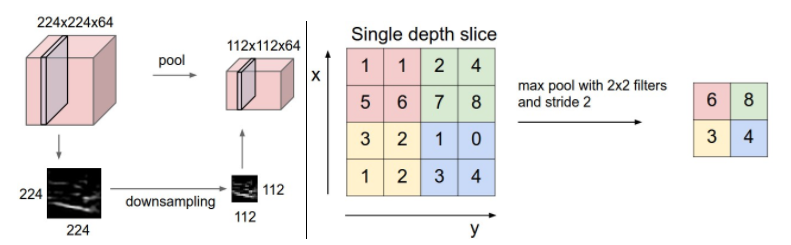
\includegraphics[width=\textwidth]{maxpool.png}
	\caption{MaxPool operation. Left: The input volume, in this example, of (224x224x64) is sliced in depth and pooled individually using \textit{filter size} and \textit{stride} set at two, resulting in a (112x112x64) volume output, keeping in mind the depth does not change. Right: With a \textit{stride} of two, the max is taken from each (2x2) matrix.}
	\label{fig:maxpool}
\end{figure}

\textit{Rectified Linear Units (ReLU)} - The activation function $f(x) = max(0, x)$ where x is the input to the neuron. This is a ramp function or \textit{rectified} function, where negative values are negated, however positive values can be large, increasing the non-linear decision function and overall network robustness. Other functions can be used, which smooth the ramp function, such as hyperbolic tangent $f(x) = tanh(x)$ or sigmoid $f(x) = (1+e^{-x})^{-1}$.

\textit{Fully Connected (FC)} - Fully connected layers means all neurons are connected to each other as in an ANN architecture. After completing the  convolution/pooling iterations a number of times, each small section of the volume is not related to the neighbouring sections, making this type of network spatially invariant. Therefore, the network must be fully connected after this process to allow a judgement based on all the information.

These layers can be manipulated, or stacked, in many different ways. Consider the operation of Convolution, ReLU activation, MaxPool, Fully connected to be be abbreviated as CONV, ReLU, POOL, and FC respectively, then the following are examples of the architectures that may be used to create the network structure:


INPUT $\Rightarrow$ CONV $\Rightarrow$ FC $\Rightarrow$ OUTPUT (Implements a linear classifier)

INPUT $\Rightarrow$ CONV $\Rightarrow$ ReLU $\Rightarrow$ POOL $\Rightarrow$ FC $\Rightarrow$ ReLU $\Rightarrow$ OUTPUT

INPUT $\Rightarrow$ [CONV $\Rightarrow$ ReLU]*2  $\Rightarrow$ POOL $\Rightarrow$ FC $\Rightarrow$ ReLU $\Rightarrow$ OUTPUT

INPUT $\Rightarrow$ [CONV $\Rightarrow$ ReLU $\Rightarrow$ POOL]*3  $\Rightarrow$ [FC $\Rightarrow$ ReLU]*2 $\Rightarrow$ OUTPUT

INPUT $\Rightarrow$ [CONV $\Rightarrow$ ReLU $\Rightarrow$ CONV $\Rightarrow$ ReLU $\Rightarrow$ POOL]*3  $\Rightarrow$ [FC $\Rightarrow$ ReLU]*2 $\Rightarrow$ OUTPUT

It can be seen that the structure could be adapted in other ways also, but it is hard to know what the best approach may be. With added layers comes added complexity and time, however the best balance of accuracy and complexity must be found.


Contrary to ANN architectures, the convolutional network is not fully connected between layers until the later stages of the process. In the ANN each neuron in each layer is connected to each neuron in the proceeding layer with associated weights and a bias value, so that the equation for each neuron is:
\begin{equation}
z = b + \sum_{i=0}^{n} w_i x_i
\end{equation}
Whereas, the convolution layer in a ConvNet only sums over the size of the feature masks. In Figure \ref{fig:conv3} the mask size is 5 x 5, an appropriate and commonly used mask size, which is represented by the following equation for the $j$, $k^{th}$ hidden neuron:
\begin{equation}
z = b + \sum_{i=n}^{4} \sum_{m=0}^{4} w_{n,m}  x_{j+n,k+m}
\end{equation}
This is advantageous when dealing with input such as high-resolution images. An ANN with an input image of resolution 128 and three RGB channels will have 128 x 128 x 3 = 49152 input neurons, leading to the same number of weights (since each neuron is fully connected) plus a bias for each hidden neuron. If the image is much larger, it can be seen that the number of variables (weights/biases) grows rapidly. However, in the ConvNet, there are only ever no more than the window size $n \cdot m$ (5 x 5 = 25 weights and one bias in the above case), for each feature mask, no matter the size of the input data.



\begin{figure}[h]
	\centering
	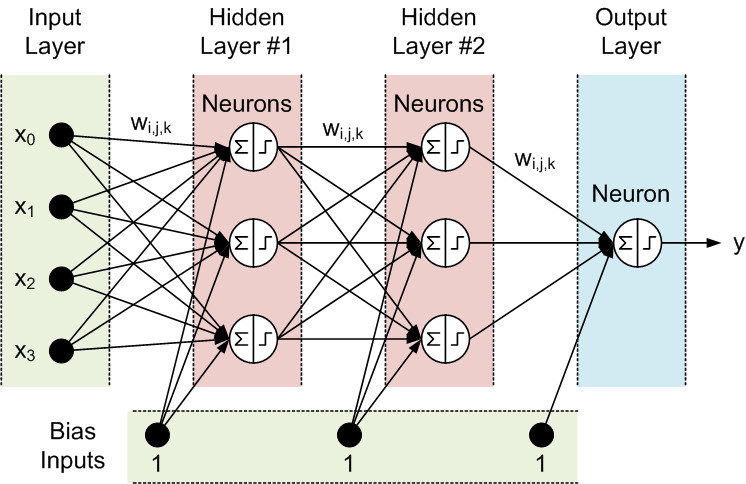
\includegraphics[width=0.8\textwidth]{neural_net.jpeg}
	\caption{Neural network topology with 2 hidden layers.}
	\label{fig:neural_net}
\end{figure}

Figure \ref{fig:neural_net} shows the flow of information through the layers in a neural network as described in \cite{smith}. Each of the inputs $Xn$ is fed to the first hidden layer with a relevant weights $W_{i,j,k}$ and biases $B_{i,j,k}$ associated for each of the neurons. Each neuron sums the weighted inputs and the value interpreted by the activation function is sent to the next layer, with yet another set of weights and biases, for each neuron. Activation functions are usually in the form of linear $y=x$, sigmoid $y=\frac{1}{1+e^{-x}}$, or hyperbolic tangent $y=\frac{1-e^{-2x}}{1+e^{-2x}}$.

Machine learning programs have been adapted in areas such as text categorization \cite{sebastiani}, handwriting recognition \cite{bottou,bahlmann}, facial recognition \cite{bartlett,bartlett2,mohammed}, medical diagnosis \cite{shipp,ye,dreiseitl}, gesture recognition \cite{lustrek,rautaray}, image classification and computer vision \cite{chapelle,ciresan,krizhevsky}, search engines and chat bots \cite{boyan,graepel,jia}, marketing/data mining \cite{cui,bose}, and an endless amount of other applications. This technology has seen rapid popularity and growth due to the flexibility and adaptiveness of such algorithms, which allows it to be used by many companies and individuals to improve systems performance. 

In recent years, self-driving cars, trucks, taxis, mining equipment, and UAVs are using ML to process images, and interpret sensor data, to recognise elements and obstacles required to operate safely. This autonomous revolution is driving machine learning research and development in great popularity \cite{lecun}. Starting with DARPA, large companies such as Google, IBM, and Microsoft have invited hobbyists, programmers, and computer scientists - anyone who has the ability - to contribute to their AI systems, processes, and libraries with solutions to problem domains they set \cite{tensorflow,cortana,udacity,xprize}.


A comparison of six deep learning architectures performed by Koirala et al \cite{koirala} in order to grade mangoes showed that all networks can perform with accuracy $>90\%$. The architectures evaluated were Faster R-CNN(VGG) (original version, and input dimension altered), R-CNN(ZF) (original version, and input dimension altered), SSD (original version, and input dimension altered), YOLOv3 (altered), YOLOv2 (original version, and input dimension altered), YOLOv2(tiny) (original version, and input dimension altered), and a specialised network based on YOLO MangoYOLO. The MangoYOLO network has slightly higher F1 score of $96.8\%$ with the inference speed at $<70ms$ for all networks using an NVIDIA GTX 1070 Ti GPU and $32GB$ of RAM.

Ma et al \cite{ma} developed a CNN to perform disease recognition among cucumber leaves including anthracnose, downy mildew, powdery mildew, and target leaf spots. The disease is more easily and less laboriously found on the leaves of the cucumber plant as opposed to the fruit itself. The team used a DCNN to perform the detection with results of $93.4\%$ which outperformed alternative algorithms such as SVM, Random Forrest, and AlexNet.

   
A Faster R-CNN network was used by Sa et al \cite{sa} to demonstrate it's adaptability of perform fruit detection in an orchard. Initially targeting sweet pepper, they fine-tuned a pre-trained network to generate bounding boxes around the fruit instances in each image achieving $F1=0.828$. Extending the work to other fruit orchard datasets with rock melon, strawberry, apple, avocado, mango and orange also delivering good results with scores of $F1=0.848$, $F1=0.948$, $F1=0.938$, $F1=0.932$, $F1=0.942$, and $F1=0.915$, respectively. 




\section{Control Systems}
\label{sec:control_sys}

Vision systems have been utilised on many production lines since the early 1980's \cite{kruger}. Computers represent a medium to perform a consistent, verifiable approach to monitoring, recording, and quality control of produced items that may be susceptible to damage, contamination, manufacturing errors, poor quality, out-of-specification features, or defects and require separation from good quality produce. Depending on the goods being monitored, there may be an option to rework, correct, repack, or remake the defected instances, therefore, the control systems will differ greatly between production lines.   

The fruit grading system by Kondo \cite{kondo} used two robot arms with 3 DOF performing a series of tasks to determine colour, size, shape, and defect. The robots alternate using suction cups to pick up 12 fruit at once in order to acquire images from the above, below, and 4 sides before pushing them into the corresponding lines. 12 camera systems in total are used, with others guiding the manipulators. This, and the project by Michalosa et al \cite{michalosa} combining mobile robots with tooled manipulators serves as examples of precision, complex, robotic control systems. However, as agricultural production line items generally are not required to be assembled or involve precise movements, control systems are relatively easy to implement, without the need for complexities such as several degrees of freedom or specialised tooling to perform the task of quality control.  

Blasco et al \cite{blasco} performed grading of pomegranate arils into five categories - White, Pink, Red, Brown, and Unwanted using several pneumatic air nozzles to eject the arils into their appropriate outlets. The system can grade a maximum of $75kg/h$ using six narrow conveyors and is highly dependant of the feeding unit to uniformly distribute the arils on the conveyor belts. As the air nozzles have a conical burst of air, incorrect rejections can occur if they are too closely distributed, or if external factors cause the arils to roll between the vision system and control. Pneumatic air ejectors helped Nouri-Ahmadabadi et al \cite{nouri-ahmadabadi} in order to grade pistachio kernels from unwanted shells. The system also required a good separation of individual items on the conveyor in order to correctly eject the affected instances. The sorter required an $8mm$ separation and could process $22.74kg/h$ with an accuracy of $94.33\%$. 

A date grading system by Al Ohali \cite{ohali} used electro-mechanical sorting strips placed at the end of the conveyors which guide the fruit into different grades. This type of control must have even larger spacing due to the mechanical movement followed by a return. Systems developed such as Sa'ad et al \cite{saad} mango shape and weight grading project used push/pull actuators to remove defect items and is akin to conveyor process control (i.e. conveyor separation, interleaving conveyors, conveyor gates, etc). Makky and Soni \cite{makky} developed a grading machine for oil palm fresh fruit bunches using stepwise discrimination in order to classify into accept and reject classes with an average success rate of $93.53\%$. Their design (and in-field implementation) employed a gate driven by a limit switch to separate the good fruit from the rejected.




\section{Summary}


A review into applications of machine vision in produce grading showed methods vary substantially depending on application and problem. Geometrical size estimation, colour, and texture analysis are common approaches due to the inherent nature of fruits and vegetables physical appearance in correlation to ripeness or maturity. However, more complicated methods have been used albeit in a more controlled environment such as laboratory settings. Vision systems provide consistent and reproducible results with advantages seen in applications where rapid production speeds, invisible spectra, lighting concerns, and seasonal variations are factors.

Size, shape, and volume can be estimated for produce items with the provision that the images are well-segmented individual, or group of items, and that the camera is fixed relative to the subject, and calibrated respectively to obtain a $pixel/mm$ measurement. This calibration can then be used to calculate length, width and shape from a single perspective, and with the addition of a camera orthogonal to the first, volumetric and 3D reconstruction can be achieved. RGB, CIE-Lab, or HSV colour spaces can provide all the relevant information required to differentiate or grade fruit and vegetables into categories of ripeness or maturity levels in with high accuracy, especially compared to the subjectivity of human quality checkers. Many fruits, for example, begin green and progress to yellow, orange, or red colours which can be exploited using CIE-Lab's $a*$ and $b*$ channels. FIS have been used successfully in grading of fruit and vegetables by implementing fuzzification methods such as PCA or binning features such as colour space, measurement, and texture reducing the classification to a simple decision tree problem.  

Selection of features is an important step in producing an accurate classification or detection model. Some results show that only a few hand-selected features can be highly accurate given the features are of significance to the deterministic characteristics of the subject. However, research also indicates that extracting and applying dozens of features may not produce a model that performs as well as others, indicating a disconnection between algorithmic and human discrimination.

Physical properties can be analysed in a non-destructive manner by way of spectroscopy - a process of measuring the internal reflectance of light through an object - using varying wavelengths in order to evaluate the internal structure, or fluorescence - measuring the excitation of an object in one wavelength, generated by a light source in another. NIR and SWIR wavelength analysis can reveal information regarding sugars, acidity, moisture, and firmness with a high level of accuracy, and thermographic and X-ray imaging has also played a part in the review. This type of analysis in the ranges of $1\mu m-15\mu m$ (SWIR/MWIR/LWIR) and $0.01nm-10nm$ (X-ray) generally take longer to process at the time of testing due to the sensor requirements with a resolution-time-cost balance used in most cases depending on application, making it difficult to employ these systems on high-speed production lines.  

The NIR region ($750nm-1000nm$), however, can be used to effectively identify defects and characteristics in objects which would be otherwise unseen by human eyes using cheap, fast, and readily available CCD and CMOS sensors. These properties can help distinguish varieties, classify grades, and detect defects with the ability to penetrate into sub-surface of skinned fruit and vegetables. Bruise detection is a common use for NIR imaging given the cameras ability to detect reflectance in the water absorption bands of the spectrum, highlighting the affected areas. This is advantageous in applications where the skin is darker than the flesh such as kiwi, potatoes, pear and apples.

Strawberries are very susceptible to damage, therefore, handling and transport becomes of concern particularly if the desire is to mechanically sort them in to categories or remove defective instances. Picking in the field and packing the berries into containers generates many opportunities to bruise or injure the delicate flesh before the quality inspection process begins. However, some progress has been made in the way of robot picking that can precisely pick and place berries into the containers using machine vision to operate the picking mechanism and perform the quality or ripeness gradation, simultaneously. Using a robot to pick a strawberry could see rates of $>10s/berry$ with current technology and is therefore mostly experimental in nature given that the volume of strawberries on a typical farm or packing room. Each method to process the strawberries in this review have been strangulated either by way of laboratory conditions, robotised harvesting, or human placement on a conveyor before the vision system assesses the quality. However, each of these options either costs more in terms of time, or labour, due to the delicate placement required in order to yield unspoiled fruit. The calyx removal system from \cite{lin} used a system of roller rods for separation of the strawberries into singular specimens before removing the calyx with a water jet. As the metal rollers apply friction to the berries in order to transport them, they are likely to have bruising and other skin damage after processing, which means the produce is no longer acceptable by retail markets, as was the purpose of their project. 

Conversely, the apples, figs, and citrus fruits reviewed have robust skin to protect them from being constantly moved, rolled, placed, and pushed during the grading and control processes. Speeds of $54,000/h$ for apples, $90kg/h$ for figs, $72,000/h$ for dates, and $5/s$ for citrus fruit have been noted proving that machine vision is currently powerful enough to process this type of volume if the automated handling is efficient and appropriate.

Machine learning and Deep learning play a vital role in produce grading, along with more naive implementations, due to their ability to discriminate between classes well. Algorithms such as LDA, QDA, SVM, ANN, BPNN may take hours to train, but can perform accurately and quickly during inference. SVM and shallow networks (such as single layer ANN or BPNN) were predominant methods to predict based on colour, size, and texture features extracted by hand, whereas, CNN and deeper networks are used where the image itself is used as input in order to predict masks or bounding boxes for identification and classification purposes.



 


%%%%%%%%%%%%%%%%%%%%%%%%%%%%%%%%%%%%%%%%%%%%%%%%%%%%%%%%%%%%%%%%%%%%%%%%%%%%%%
%%%%%%%%%%%%%%%%%%%%%%%%%%%%%%%%%%%%%%%%%%%%%%%%%%%%%%%%%%%%%%%%%%%%%%%%%%%%%%
\newpage

\chapter{Strawberry Inspection System Design}
\label{sec:I}


\section{Introduction}


In order to develop a successful strawberry inspection system, the techniques used to illuminate, acquire, and process images is of significant importance as they will determine the quality of imaging, therefore accuracy of assessment. The following section examines the limitations and constraints of processing in production including throughput, lighting, reflections, and imaging, indicating the critical system requirements for operational success. Robust solutions supporting the requirements must be sought in order to develop a production-ready system that can deliver the necessary outcomes in a demonstrably consistent and accurate manner, according to the expectations of Magnificent Pty. Ltd.

The second part of this chapter discusses and presents the findings drawn from experimentation with the main components of the system. Testing lighting conditions at fast shutter speeds is an important aim of the testing phase and will determine intensity, minimum shutter speed to avoid blurring, camera settings, polarisation and diffusion. These environmental variables are crucial considerations which will impact on image quality, and must therefore be optimised. Software and hardware development (including control systems) are investigated to facilitate the removal of defects, provide a user interface, and perform the assessment of acquired images.


\section{Design Considerations and Constraint Analysis}
\label{sec:challenges}


The design of the system is based on the requirements detailed in Chapter \ref{sec:requirements} such as footprint, safety, power and compressed air usage, and continuity. Added to this are some underlying assumptions and design requests from Magnificent, given their previous project experience which has provided the company with knowledge and tools to assist the development of the new system. Past projects include a field robot designed to traverse the rows of strawberries planted and pick ripened fruit. This project provided experience in $12V-24V$ circuits and power design, high power LED illumination and camera positioning and registration. A second project consisted of a picking robot in a vertical greenhouse (where the robot was fixed to single dimension axis on rails and the strawberry troughs rotated to bring the fruit within picking range), developed more accurate grading, polarization of the LED light, and camera registration and synchronisation. Building on this experience, aspects from these projects can be applied to the system being developed including polarisation techniques, camera characterisation, power systems, and software packages.

These considerations and others are detailed below, along with limitations of the system environment such as line speed, illumination, and camera configuration, in order to ensure the design is compatible and corresponds to the requirements. 


\subsection{Specular Reflections}

Specular reflections occur when the viewer is in the path of directly reflected light from a source. In other words, the light source can be seen on the surface of an object, reflecting the spectrum of the source, which can add unnecessary noise to images resulting in loss of information, as shown by the white reflective pixels on the otherwise red strawberries in Figure \ref{fig:strawberry_glare}\cite{gurney}. Given that the strawberry flesh's refractive index is great than air, the incident and reflected angles will not be the same. However, as the strawberry is curved in multiple directions, and has surface elements of different sizes, many specularities occur. 

\begin{figure}[h]
	\centering
	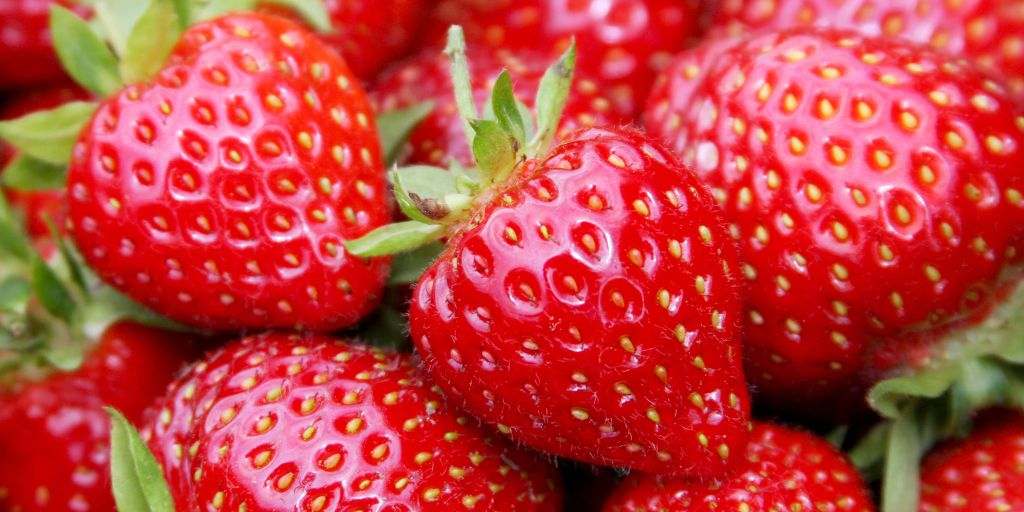
\includegraphics[width=.6\linewidth]{strawberry_glare.jpg}
	\caption{Strawberries with dominant specular reflections reducing the ability to analyse pixels}
	\label{fig:strawberry_glare}
\end{figure}%

There are a few methods to combat the specular reflections, such as polarizing the light, changing the angle of the source, or diffuse lighting. In the case of this project, all three are investigated in order to reduce the specularities to a minimum. 

Polariser material had been advantageous in previous projects given the various lighting conditions, both outdoors and within a greenhouse by way of reducing glare. However, specular reflections are an inherent property of strawberries due to their pitted exterior, effectively making small crater-shaped edges that can cause specularities from any angle. Figure \ref{fig:strawberry_glare} shows a number of white areas around the seeds caused by direct reflection of the light source. As the craters are round, and the berry's surface is curved in three dimensions, the specular reflections are unavoidable.


\subsection{Polarisation}


Polarization of a light source (using a polaroid sheet) will reduce the overall light intensity by a factor of $\frac{1}{2}$ due to Malus' law given by
\begin{equation}
I = I_{0} cos^{2}\theta_{i}
\end{equation}

with $I_{0}$ being the initial intensity and $\theta_{i}$ is the angle of the polariser axis from the angle of initial polarization. If a light source is unpolarized, it is assumed to have a combination of all polarization directions and so $cos^{2}\theta$ is averaged to $\frac{1}{2}$. Although, in practice, this figure is less due to imperfections in polarizing material, more light will be required in order to achieve the same luminosity on the subject \cite{rox, sommer} whilst reducing/removing the intense reflections. Specularities appear the same colour as the light source, which in most cases is white, effectively 'blinding' the cameras from true information behind the glare.  


Polarization is the process of converting electromagnetic waves of varying polarity into a uniformly polarized field. Usually used for visible light or lasers, polarisers can reduce glare (for example, polarized sunglasses) or help in the amplification and directionality of lasers. Figure \ref{fig:polarization} illustrates the polarization of an EM wave, indicating that no matter the intensity of any direction, only a single polarity emerges  \cite{physicsopenlab}. Using a polariser is an effective technique to reduce glare from a flat surface (polarized sunglasses are assumed to be worn horizontally, using vertical polarization in the lenses in order to block glare from horizontal surfaces such as water and concrete), but will be mostly ineffective for the curved surface of the strawberries. However, using cross-polarization (two polarisers orthogonal in direction) in order to reduce these reflections is considered, even though this will limit the amount of illumination reaching the subject significantly.

\begin{figure}[h]
	\centering
	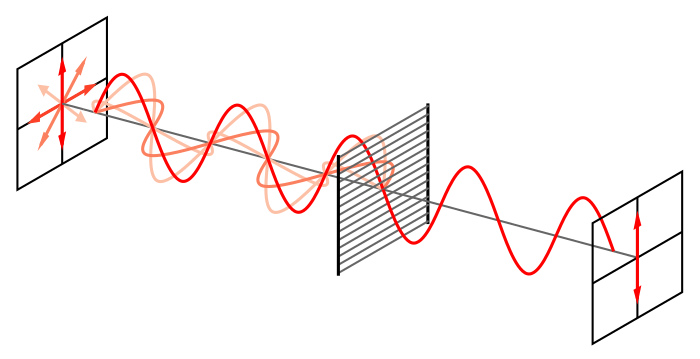
\includegraphics[width=.8\linewidth]{polarization.png}
	\caption{Electromagnetic polarization. A circular or randomly polarized source becomes a single polarity after passing through the material.}
	\label{fig:polarization}
\end{figure}%


\subsection{Illumination Source}

As this project would take advantage of the NIR spectrum with the intention of capturing bruising or other invisible defects, the light sources must be capable of generating the required illumination. Previous projects used LED sources as they are more efficient and can be operated using $12V$ power, but are generally limited to small bands of radiation. Some LED manufacturers claim to generate a high Colour Rendering Index (CRI), which is a measure of the comparison to natural light. However these LED's generally do not output wavelengths greater than $750nm$ as there is no need in most cases, which is much of the reason they are more efficient in terms of power. Figure \ref{fig:LED_response} plots the power distribution of the Cree\textregistered CXB3590 LED's spectrum over four different colour temperatures confirming the absence of NIR wavelengths \cite{led_power}. This means that LED's may not be useful and a more appropriate light source such as halogen or tungsten must be used.


\begin{figure}[h]
	\centering
	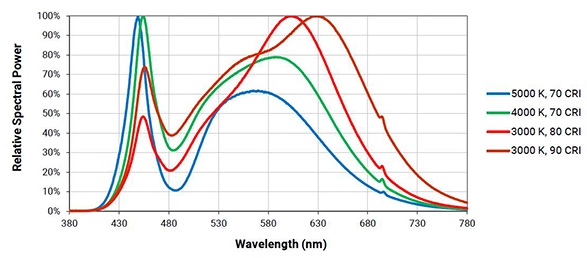
\includegraphics[width=.9\linewidth]{LED_response.png}
	\caption{Cree CXB3590 power distribution curves for a range of colour temperatures at $T=85^{\circ}C$.}
	\label{fig:LED_response}
\end{figure}%





\subsection{Punnet Imaging}

Due to processing restrictions, it is a requirement that the punnets be imaged from top and bottom simultaneously, therefore requiring an obstruction-free conveyor system to transport punnets through the acquisition section. This can accomplished by using the lip of the punnet (around the top of the container) as a handle point where thin v-belts can suspend the punnets giving little visible impact to the scene and allowing full view of both the top and bottom, simultaneously.

Shiv Ram Dubey and Anand Singh Jalal \cite{shiv} investigated fruits and vegetables as well as some fruit diseases using a multi-class SVM classifier as a solution. Qiang LÜ and Mingjie TANG \cite{lu} devised a method for identifying Kiwi fruit, which had hidden bruises under the skin, by using hyper-spectral imaging and a parallelepiped classification approach. These experiments, as well as other work \cite{elmasry2,chiu}, have used a static imaging system. That is, the subject was stationary and usually had a clean, flat, un-obscured background that makes the process of segmentation quite trivial. 

However, the system described in this report requires images to be taken of full punnets as they move down the production line. The line speed of production equates to two punnets per second and leaves little room for camera setting adjustments such as shutter speed and gain. Additionally, the strawberries will be located inside a plastic punnet and may result in poor images due to the following:  

\begin{itemize}
	\item Punnet wall reflections - light may reflect from the strawberries and project a mirror-like reflection on the inside punnet wall. These reflections could lead to false positive rejects, as they will be transformed in colour, shape, and texture.
	\item Multiple occlusions - strawberries are tumble packed and are usually more than one layer, therefore, the fruit located on the top most layer will almost certainly occlude the berries on the bottom of the punnet. 
	\item Shadows - when the fruit is tumble packed, it can form many shadowy areas, particularly on the lower layer. The berries on top will sometimes block light from other berries, casting shadows which may inhibit assessment.
	\item Poor berry orientation - tumble packing means that the berries inside the punnet could be in any orientation. As the image will be taken from above, it could be hard to tell whether a berry is lying on its side or end. The strawberry calyx could also be clearly visible and obscuring the view of that, and potentially, other berries. 
\end{itemize}

These added problems will detriment the image processing algorithms. Morphology is challenging due to the occlusions and shadows, and colour will be difficult to assess, as the shadowy lower fruit will be darker than fruit in full light. Measurement of berries may not be completely accurate as the occlusions, shadows, and orientation will dictate the accuracy of this process.


\subsection{Flickering}

As the strawberry punnets pass along the production line at a rapid pace, the shutter speed of any cameras used will need to be able to capture without blurring, but with enough light to illuminate the berries to the desired levels. The fast shutter speed requires high-powered lighting in order to allow the sensor to accumulate enough photons in such a short amount of time.

High-powered lighting is generally in the form of 110V/220V AC powered lamps which can generate over $1000W$, however, the alternating current poses the problem of flickering. This occurs when the shutter speed of the camera is faster than the time taken for a $\frac{1}{2}$ revolution of the AC sinusoid (given that the positive and negative current flows produce the same power). In a region where the AC power is specified as $50Hz$ the time taken for one period is: 
\begin{equation}
T_{AC} = \frac{1}{f} = \frac{1}{50} = 0.02 = 20ms
\end{equation}


Taking half of this period, the minimum shutter speed time is 10 milliseconds. Any shutter speed greater than this ($1/100$) will display signs of flickering due to the inconsistent amount of photons gathered each cycle. 


\begin{figure}[h]
	\centering
	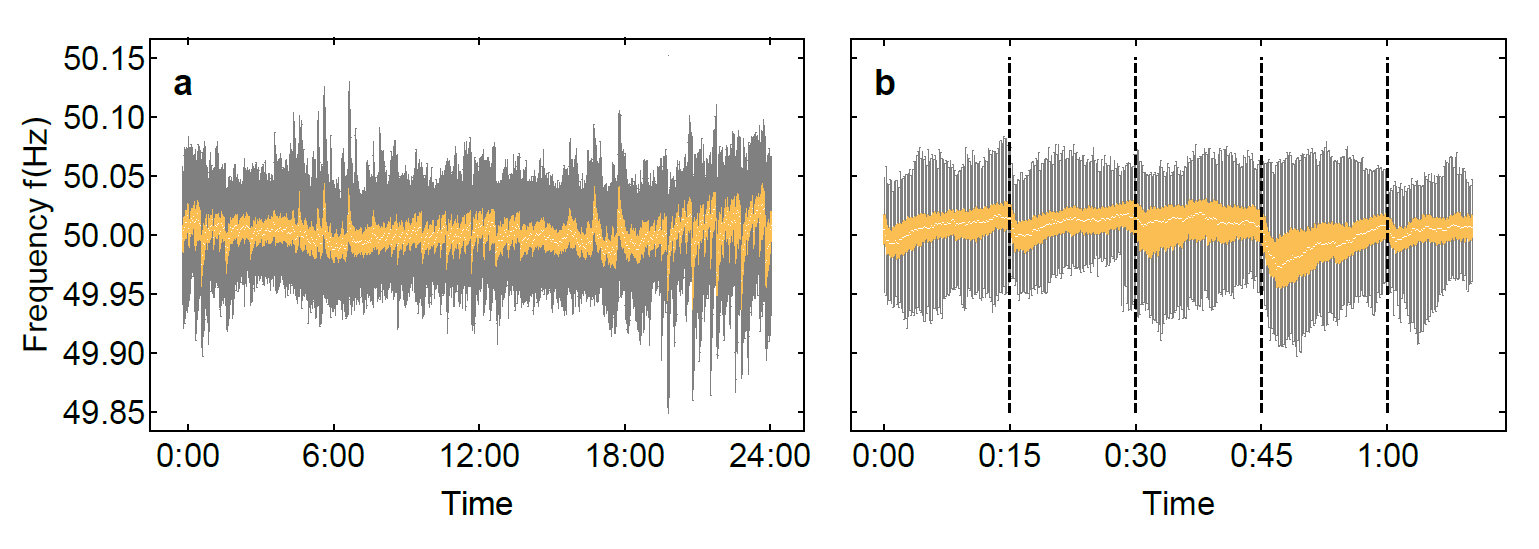
\includegraphics[width=0.9\textwidth]{50hz.jpg}
	\caption{Fluctuations recorded for 50Hz nominal AC power signal - European grid (2015) samples of (a) 24 hour period, and (b) 15 minute intervals.}
	\label{fig:50hz}
\end{figure}

Strategies such as shutter synchronisation (with the AC signal, in an attempt to open the shutter at a relative rate) can be employed, however the mains power frequency can decrease and increase by small amounts due to supply/demand fluctuations. The graph in Figure \ref{fig:50hz} reinforces the fact that inconsistencies are ongoing due to the constant change in demographic power requirements \cite{50hz}.

\begin{figure}[h]
	\centering
	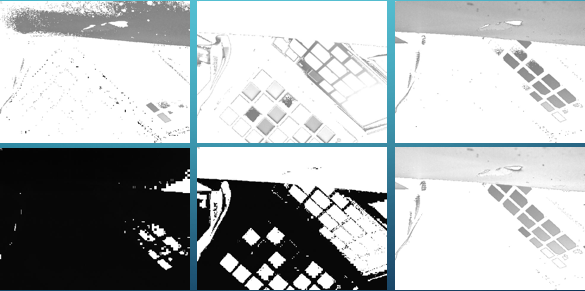
\includegraphics[width=0.8\textwidth]{flicker.png}
	\caption{Six images taken using identical properties ($5ms$ shutter speed), and threshold values, at varying times within one second using AC-powered light source.}
	\label{fig:flicker}
\end{figure}





If the shutter speed is fast, the sensor can be exposed to maximum light, when the light source current reaches maximum, or theoretically, no light at all when crossing the 0V point in the alternating cycle. Some examples of sparse region differences are shown in Figure \ref{fig:flicker} with images acquired using static camera and algorithm parameters, where only time was varied.


\subsection{Software Framework}

Both of the above mentioned previous projects made use of software frameworks such as Microsoft's Visual Studio\textregistered for application design, GUI, debugging, and deployment. Additionally, a licence for MVTec Software GmbH's HALCON\texttrademark had previously been purchased with a knowledge base established, therefore the use of these frameworks was requested by Magnificent due to the successful implementation in past projects, availability, and ease of use.

Visual Studio\textregistered is an Integrated Development Environment (IDE) designed for applications based in $C\#$ or $C++$ programming languages predominantly. It provides project configuration tools, automatic library attachment, a GUI designer and linker tool which can increase the speed of development and facilitate changes and updates in an agile manner. Although it is free to use for development under the Community edition, commercial distribution would be subject to enterprise licence. 

HALCON\texttrademark uses it's own programming language and IDE to create applications, and has the power to speed up development by implementing a vast library of common image processing functions. The IDE contains several visualisation windows such as code editor, current image (overlayed with current operational markers), and a window displaying all the objects created in the program including regions, images, colour channel operation steps, and contours as well as a list of control variables (integers, arrays, floats, etc.) and their values if set. As the variables are cached in a database during development, the user can interactively adjust parameters or functions and see the results by simply re-running the relevant lines of code, with the resulting changes visualised instantly. The HALCON\texttrademark application code can be converted directly to $C\#$ or $C++$ code in order for integration into commercial applications such as Visual Studio\textregistered. As Magnificent had a pre-existing licence for this software, the efficiency increases, and compatibility of both software packages, any future development was to undertaken utilising the existing framework portfolio.


\subsection{Asynchronous Acquisition}

As mentioned in Chapter \ref{sec:requirements}, there will be four images acquired for each punnet that passes through the enclosure, meaning that the application in control of the cameras must be able to collate four images, taken at different times.

Due to the large number of punnets flowing through production, the likelihood of a constant stream of punnets is high (i.e. little or no space between them). This means that the cameras must be able to operate individually in order to prevent the sequential scenario where an image is missed or delayed due to the previous. The application will then need to collate these images in order to save them in a defined storage device, preserving production quality traceability.    

\subsection{Processing Time}

Since the introduction of the heat-seal machine, the production line has been sped up to almost the maximum capable ($120$ punnets per minute), in order to increase throughput. This equates to two punnets per second or $500ms$ per punnet which must allow detection, capture, processing, and decision making. Therefore, the processing time may be as little as $300-400ms$, which limits the ability to solve complex or inefficient algorithms. State-of-the-art classifiers can take more time to perform evaluations with simple classifiers taking a few seconds in some examples. This will require careful consideration if each punnet is to be assessed, and will be addressed in later chapters.


\subsection{Motion Blur}

The conveyor line speed of 16.8 meters per minute, or 28 centimetres per second, allows for up to two punnets per second to transit the enclosure. If the camera's shutter is left open too long, the moving object will become blurred due to the spacial displacement which occurs during image integration. This leads to smoothed edges, a blurred overall appearance, reduced precision, and potential false artefacts which could influence the performance of the algorithms.



\subsection{Orientation of Punnets}

The strawberry punnet heat-seal machine has been designed to be as efficient as possible, which means that for maximum efficiency, more punnets should be sealed at the same time. As the strawberry punnets are rectangular, this means that they must be long edge leading into the sealer in order to be able to seal five punnets at a time rather than four. This increases the rate of the punnet sealing from 100 to 120 per minute, giving accelerated throughput gains, but raises problems elsewhere in the production line. 

As the vision system feeds in-line into the heat-sealer, the vision system must also process the punnets with long edge leading. Since the punnets are transported through the enclosure by suspension on thin v-belts using only the lip of the plastic punnet, it will simply fall into the bottom of the enclosure if the punnet was wrongly oriented. The packing staff need to correctly orient the punnets on the packing line so that they enter the vision enclosure correctly. However, this may be difficult to sustain, given packers are quite rushed due to the fact that they are remunerated relative to the amount of punnets packed. Therefore a fail-safe system must be devised in order to either ensure that the punnets are correctly oriented before they reach the enclosure, or there is a sensor/detection unit which will alert operators if the situation arises.


\subsection{Overheating}

Lighting for the cameras must have enough power to illuminate the subjects with a fast shutter speed due to the fast-paced throughput. Although high powered lighting is required, this can create other problems such as overheating, causing damage to other components, and a potential safety hazard. Focusing the lighting directly onto the strawberries may cause specularities, diminishing the information collected by the cameras, and therefore must be diffused in some way. The lighting must also emit wavelengths of importance, such as visible and IR so that these wavelengths can be viewed through the cameras, meaning increased lighting power and therefore heat.



\subsection{Ejector Synchronization}

A pneumatic ejection system will remove the defective containers from the production line. Research in Chapter \ref{sec:control_sys} indicates this is a common practice in agricultural vision systems and is facilitated by the air system provided in the requirements list. As the strawberries are already packaged when entering the vision system, the entire punnet will be ejected, so that it may be repacked and re-analysed by the system.

The ejection system is attached to the production line outside the enclosure, and therefore requires it's own punnet sensor in order to eject a punnet as it moves past the pneumatic manifold (aperture). Added to this, the punnet sensor inside the enclosure must be perfectly synchronised to the punnet sensor at the ejector so the correctly identified reject punnet is ejected and not an adjacent punnet. The ejector accuracy is proof in the system for operators and must be able to correctly eject the failed punnets for inspection, otherwise confidence in the system will reduce.


\subsection{Conveyor Motion}

The punnet heat-seal machine is designed to seal five punnets at a time and is therefore not in constant motion. It has a sensor at the infeed to the sealer which tells the machine when the required amount of punnets have passed into the sealing apparatus. This sensor may also stop the infeed line (approximately 1-2 seconds), to prevent more punnets entering. The conveyors into and out of the enclosure are controlled by this mechanism as well. This is to ensure that if there is a problem in the heat-seal machine, and operators use the e-stop or safety switches monitoring the access doors to stop the production line, the enclosure conveyors stop as well.

However, this means that the conveyors could stop at any time during the sensing, acquisition, and ejection phases of the vision system. Therefore, time-determinant processes (such as using a finite time delay between camera sensors, or camera and ejector sensors) will not be sufficient. Other factors may need to be addressed due to this motion, such as inertial sliding, sensor miss-triggers, image positioning, and independent software processes in order to handle operations in a modular process. 



\section{Strawberry Quality Assurance (SQA) System Design}


The Computer Aided Design (CAD) generated cross-section of the proposed SQA system in Figure \ref{fig:cross_sec} illustrates the concept of the conveyors (in-feed, out-feed, and v-belt), placement of cameras and PC, as well as the polariser sheets. This illustration integrates the already existing frame constructed for the prototype, therefore the prototype could be retrofitted to include in-feed and out-feed conveyors, and the v-belt system.  



\begin{figure}[h]
	\centering
	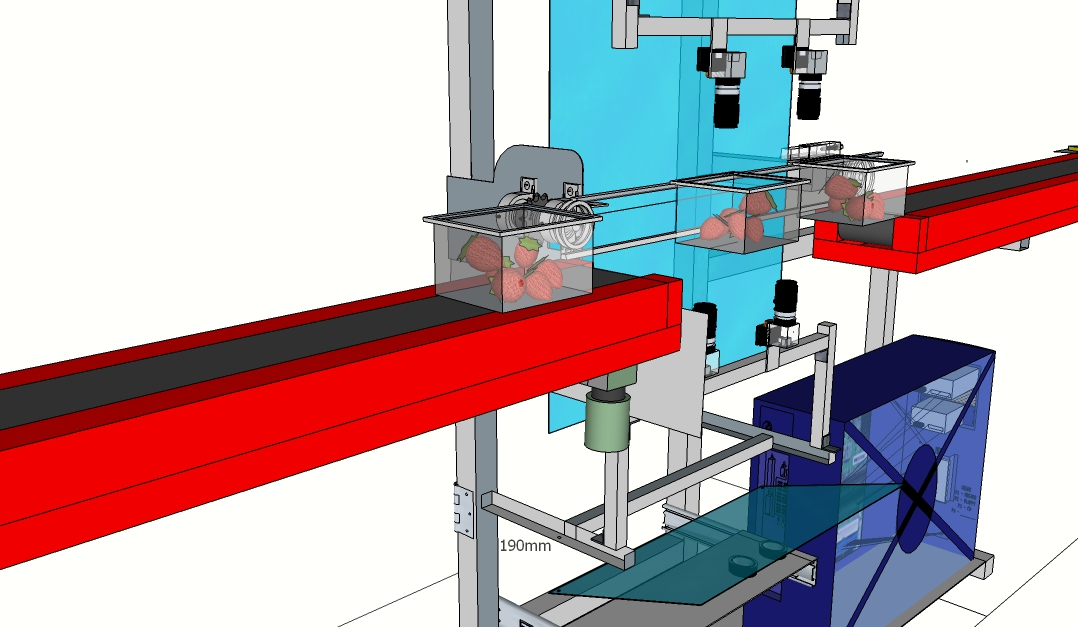
\includegraphics[width=.8\linewidth]{QAS_cross_sec.jpg}
	\caption{Cross-section of the SQA system illustrating the polarizing filter (blue sheet), the v-belts, and four cameras in position above and below.}
	\label{fig:cross_sec}
\end{figure}%



The PC is placed under the out-feed conveyor (as there is less probability of impact hazard), and runs the master program which controls every peripheral including cameras, peltier devices and fans, pneumatics, operator controls, image processing, and GUI. The microprocessor is a stand-alone industrial board (Phidget\texttrademark) and controls the I/O as described in Section \ref{sec:phidget}.

As indicated in the requirements (Section \ref{sec:requirements}), the farm packing facility will provide power of either $240VAC$ - single phase, or $400VAC$ - three phase as well as a single compressed air line. However, the system is designed to use only $240VAC$ as higher power is not required by any function, including the conveyor motors.


\subsection{Prototype Construction}
\label{sec:prototype_contruct}


The enclosure was firstly constructed offline as a bench prototype (Fig. \ref{fig:bench_construct}), in order to test lighting arrangements, polarisers, and cameras. This prototype was then used as the framework when moved from bench to production. The frame is constructed from aluminium modular T-slot ($20mmx20mm$) components, supports stainless steel sheets that are moulded to be curved on top and bottom in order to diffuse and direct light and reduce flat surface reflections whilst creating a more evenly distributed background and intensity. Front and back panel doors allow access for staging and adjustments but block the outside light interference. This was performed with the intention to reproduce the environment of a fully enclosed system installed on the production line. 

\begin{wrapfigure}{r}{0.5\textwidth}
	\begin{center}
		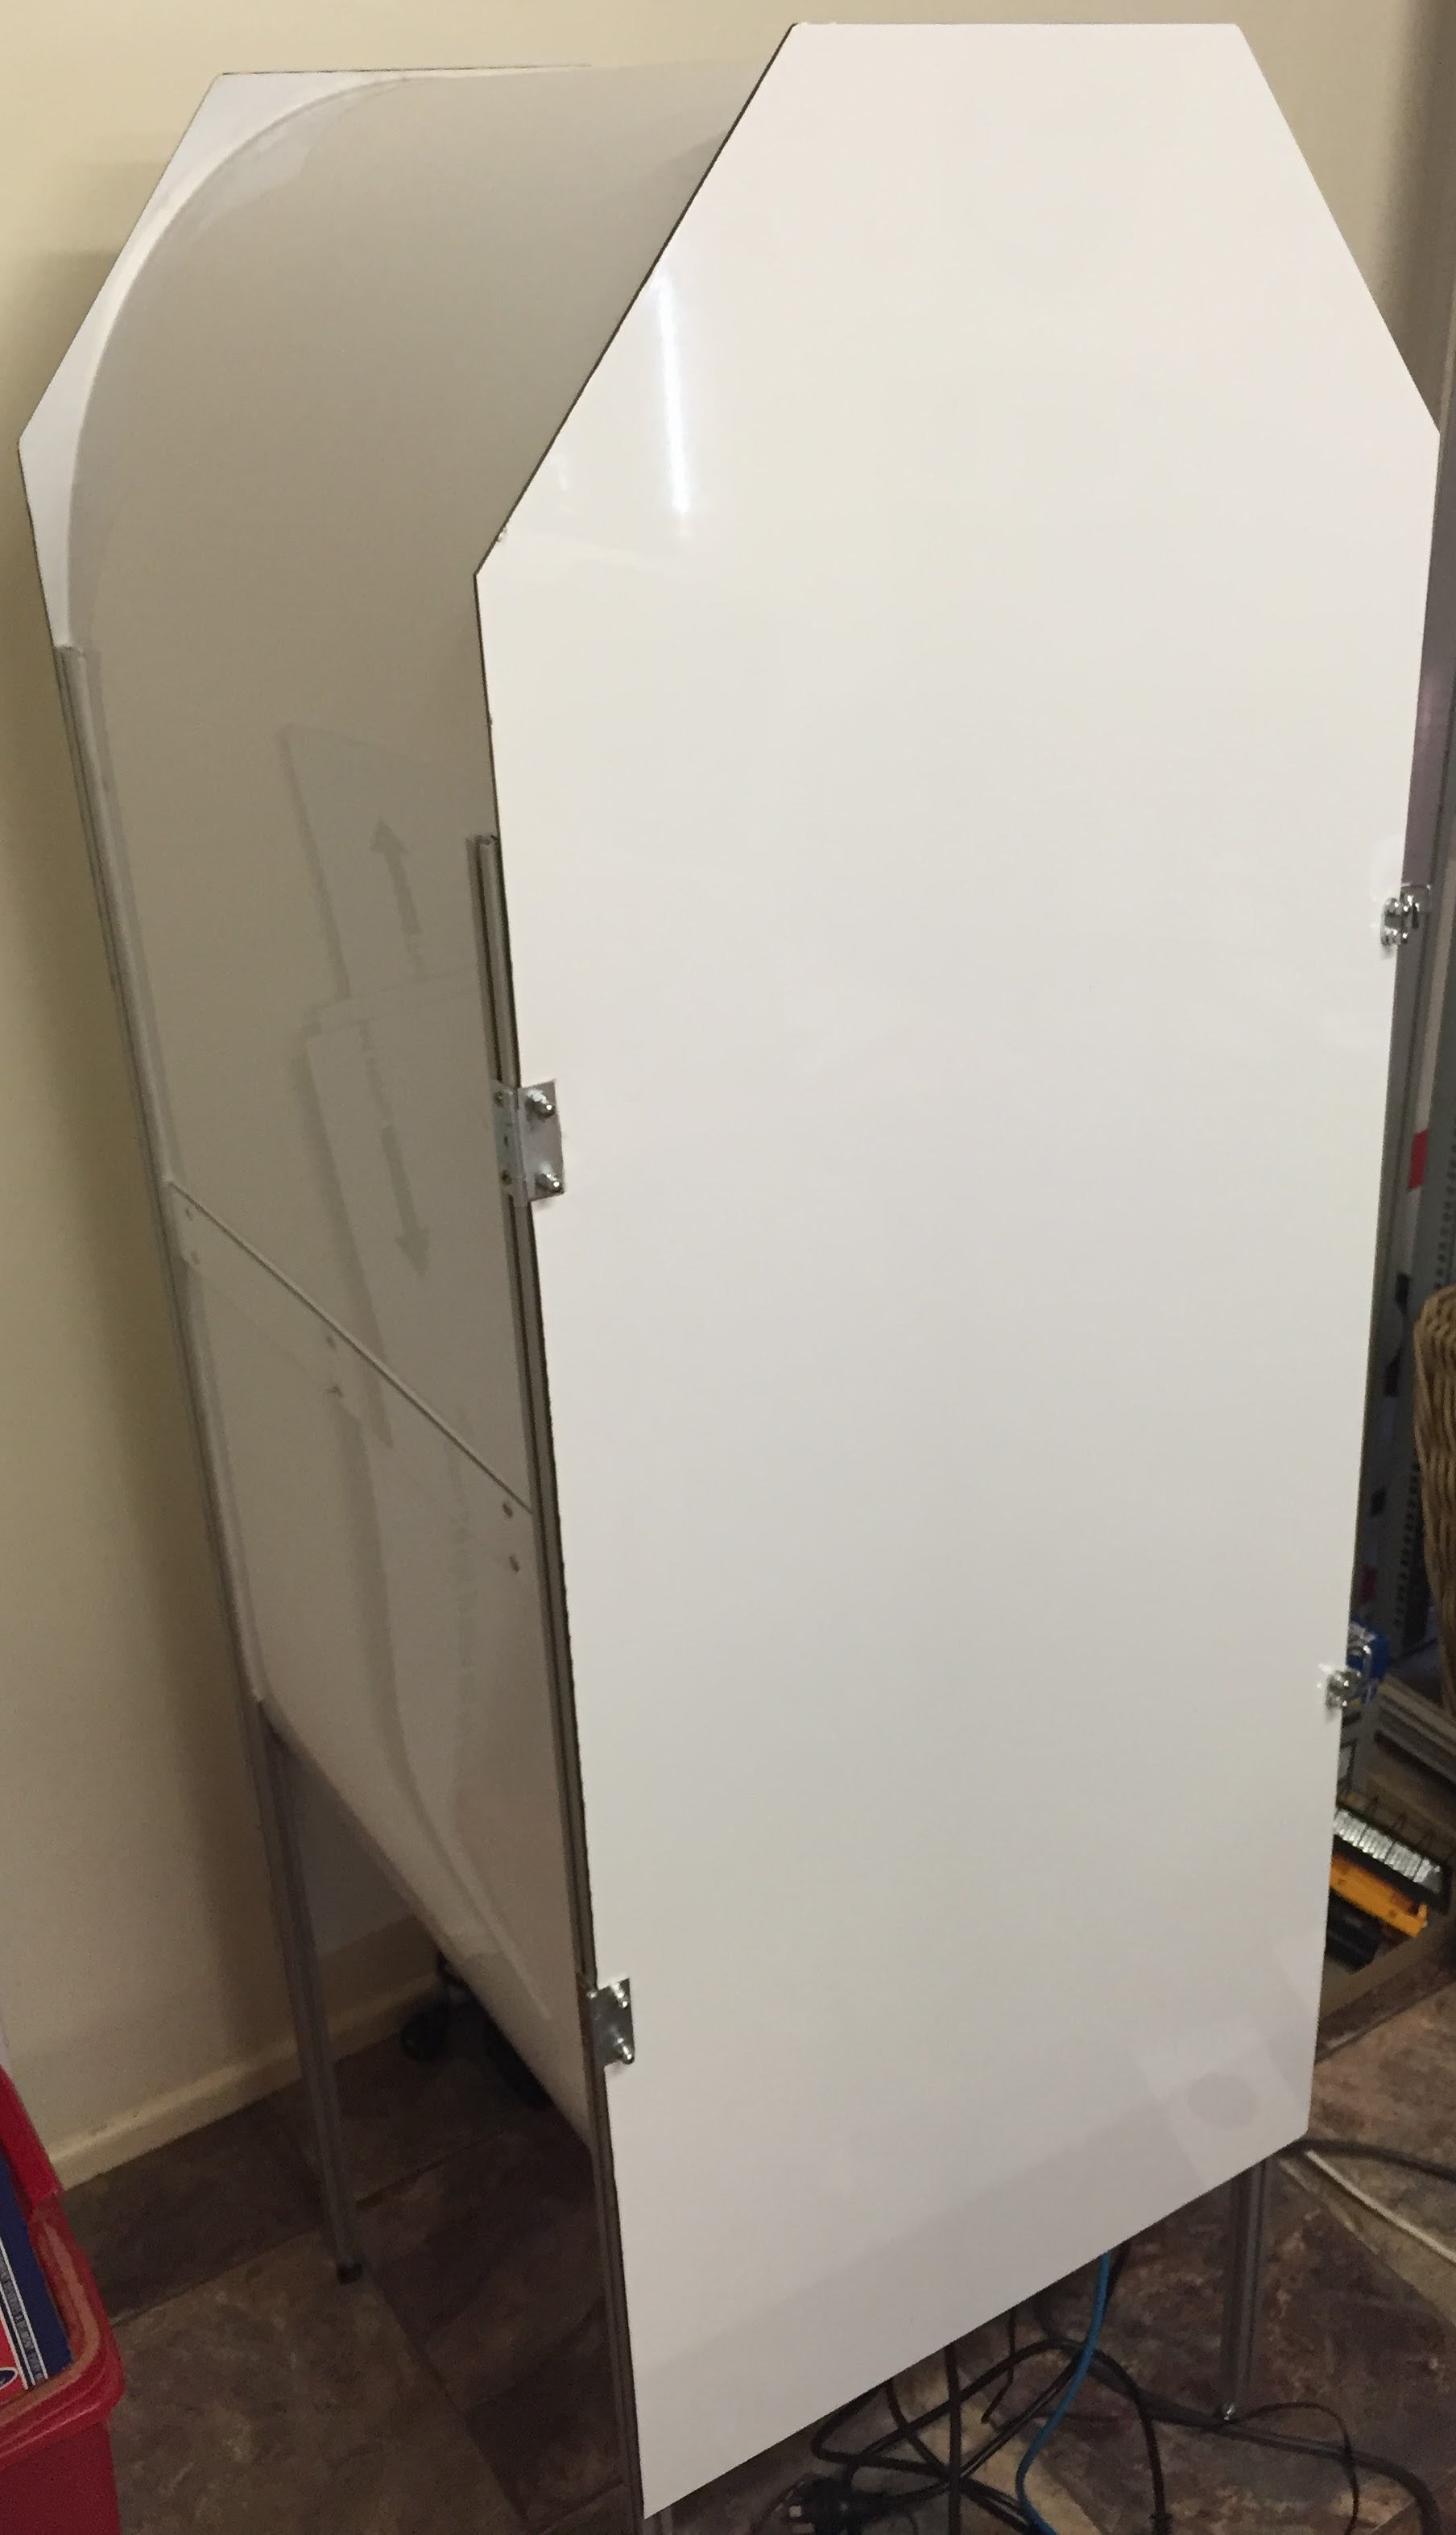
\includegraphics[width=0.3\textwidth]{images/bench_construct.jpg}
	\end{center}
	\caption{The enclosed prototype during construction and testing.}
	\label{fig:bench_construct}
\end{wrapfigure} 

 

The design of the frame and doors included the ability to manoeuvre lighting mounts, cameras, diffusers, and image targets easily by opening each side of the enclosure to position the relevant components. T-slots along the length of the framework uprights and cross supports allowed cameras and lighting to have two degrees of movement (in the horizontal plane) for positioning. 

Even though many assumptions and considerations can be used to design and construct a lighting system (particularly industrial), the resultant images may not be as expected. Problems due to real-world constraints (processing rates, power constraints, environmental factors), or unexpected effects (reflections and shadows, camera characteristics, configuration problems) can contribute to considerable rework and waste if not tested. Prototyping is used to provide proof-of-concept before committing to financial investment and production disruption.



\subsection{Illumination Intensity}

Illumination intensity, lighting type, and configuration are of high importance when acquiring images, and can mean the difference between poor and excellent algorithm results \cite{lorente,kondo,liu2}. This is due to various effects such as diminished intensity, reflections and hotspots, shadows and voids, inconsistency, spectral range, and directionality. Given the production application of the system, lighting attributes are of greater importance given the duration of production can be more than 12 hours, line speeds are continuous and fast-paced, and multiple berries will be assessed with each image.

Minimum Illumination is a term (typically used for CCTV cameras) that is not clearly defined, but is used to describe the minimum amount of light required in order to distinguish the objects in the image \cite{min_illumination}. This is difficult to compare for a few reasons, namely, differences in reflectivity of the objects, the display screen, where the light reading is taken from, and how it is measured, as well as the fact that human eyes are unique, therefore subjective in terms of distinguishing features. 

Luminous intensity ($I$) describes a light source's omnidirectional energy, measured in units of candela ($cd$), where $1cd$ was originally defined as the amount of light produced from one candle, but has been more precisely defined since 1948\cite{light_units}. Dividing the total luminous intensity by $4\pi$ (as there are $4\pi$ steradians to a sphere) is a measurement luminous flux ($F$) whose units are lumen ($lm$). One lumen is produced by a luminous intensity of $1cd$ over one steradian, and is typically used by light manufacturers to describe the amount of directional illumination emitted by their devices.

Therefore, the definition of luminous flux is:
\begin{equation}
	F = I\cdot\omega
\end{equation}

where the angle ($\omega$) can be expressed as a function of area $A$ and distance $d$ from the source, given a constant source of light:
\begin{equation}
	\omega = \frac{A}{d^2}
\end{equation}

This shows the intensity is inversely proportional to the square of the distance, but distances inside the enclosure are not consistent given the reflectance from the curved inner walls. Calculus problems of this type can offer solutions, however given the complexity of the inner structure of the system (including cross-polarisation), the intensity requirements will be established with less effort through experimentation. 




\subsection{Lighting}
\label{sec:lighting}

Halogen work lamps supplied lighting as they were capable of emitting the full spectrum required for both the RGB and IR imaging systems. They are readily available, with power up to $500W$ per lamp and a footprint small enough to fit eight inside the enclosure. Several lighting and polarizing configurations were tested (using a thin film type polaroid) for optimization (Figures \ref{fig:bench_hal_film} and \ref{fig:bench_hal_film2}), before the AC flickering problem was realised. This test was successful in proving that the polariser reduced specularities, and that powerful lighting was required, however, it highlighted the inherent problem with AC lighting and fast shutter speeds. It was also noted during these preliminary tests that the polariser film would be less effective when bent or warped. 


\begin{figure}[h]
	\centering
	\begin{subfigure}{.45\textwidth}
		\centering
		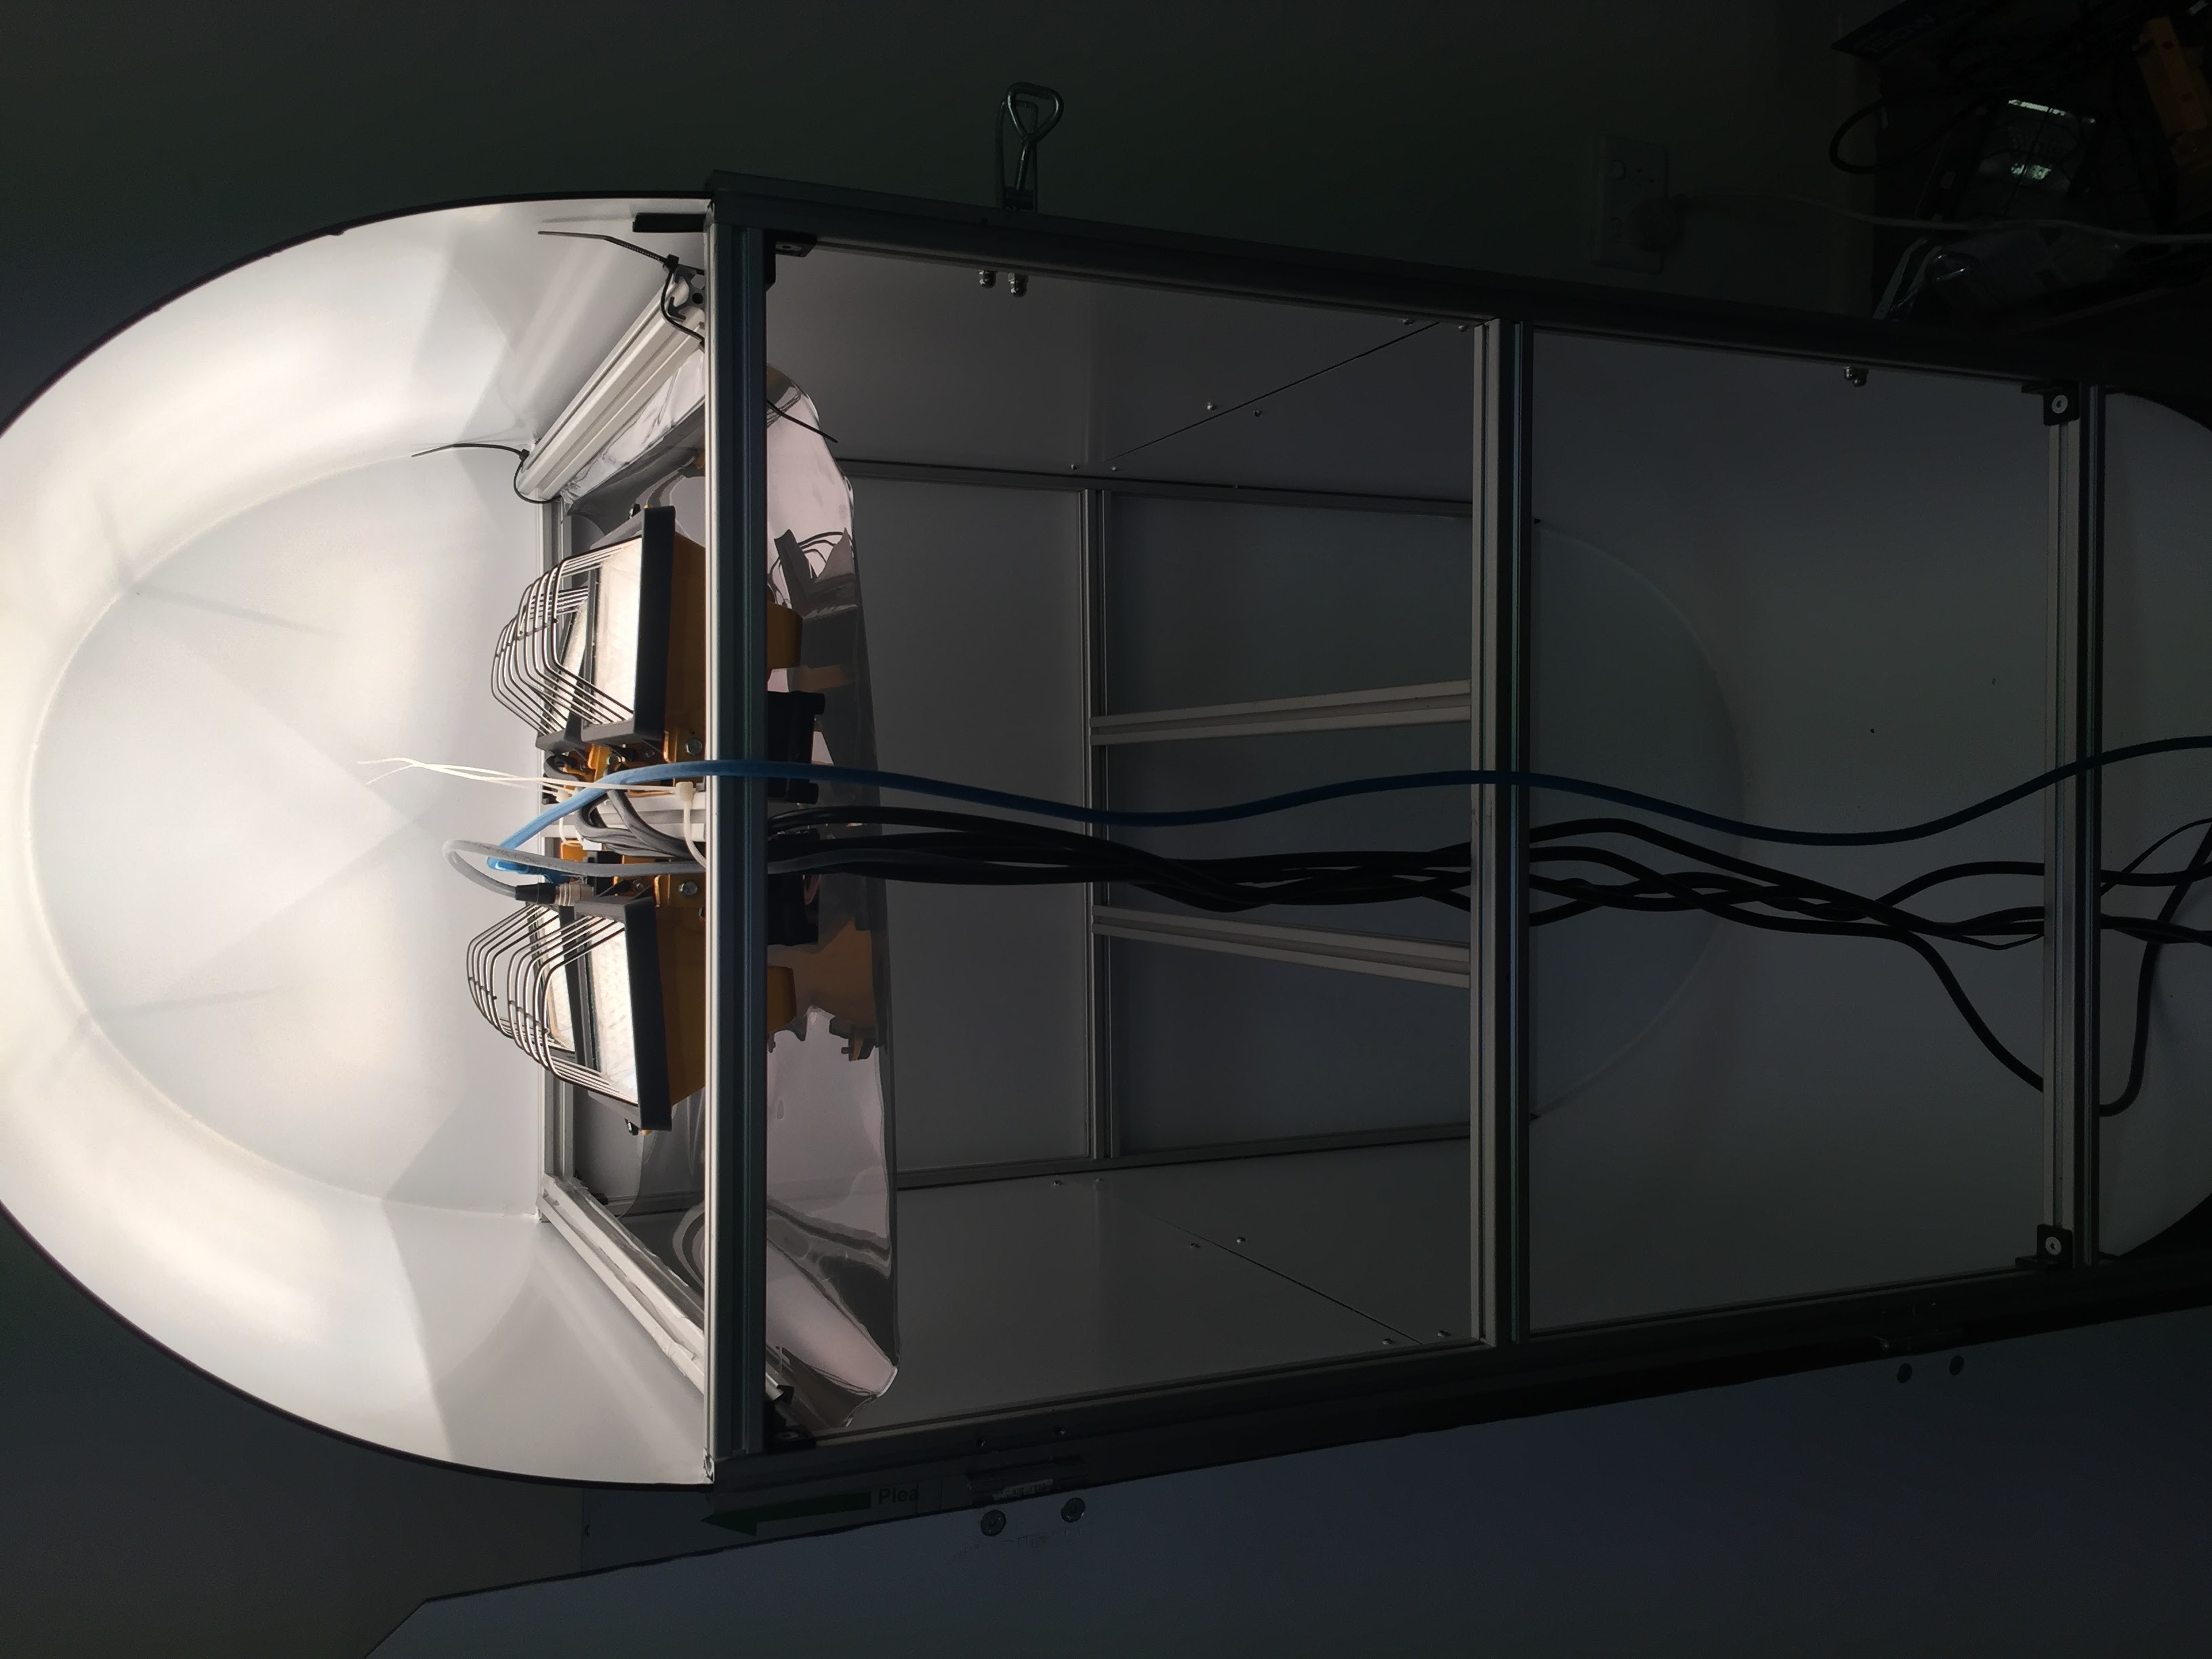
\includegraphics[width=\linewidth,angle=270,origin=c]{bench_hal_film.jpg}
		\caption{}
		\label{fig:bench_hal_film}
	\end{subfigure}%
	\begin{subfigure}{.45\textwidth}
		\centering
		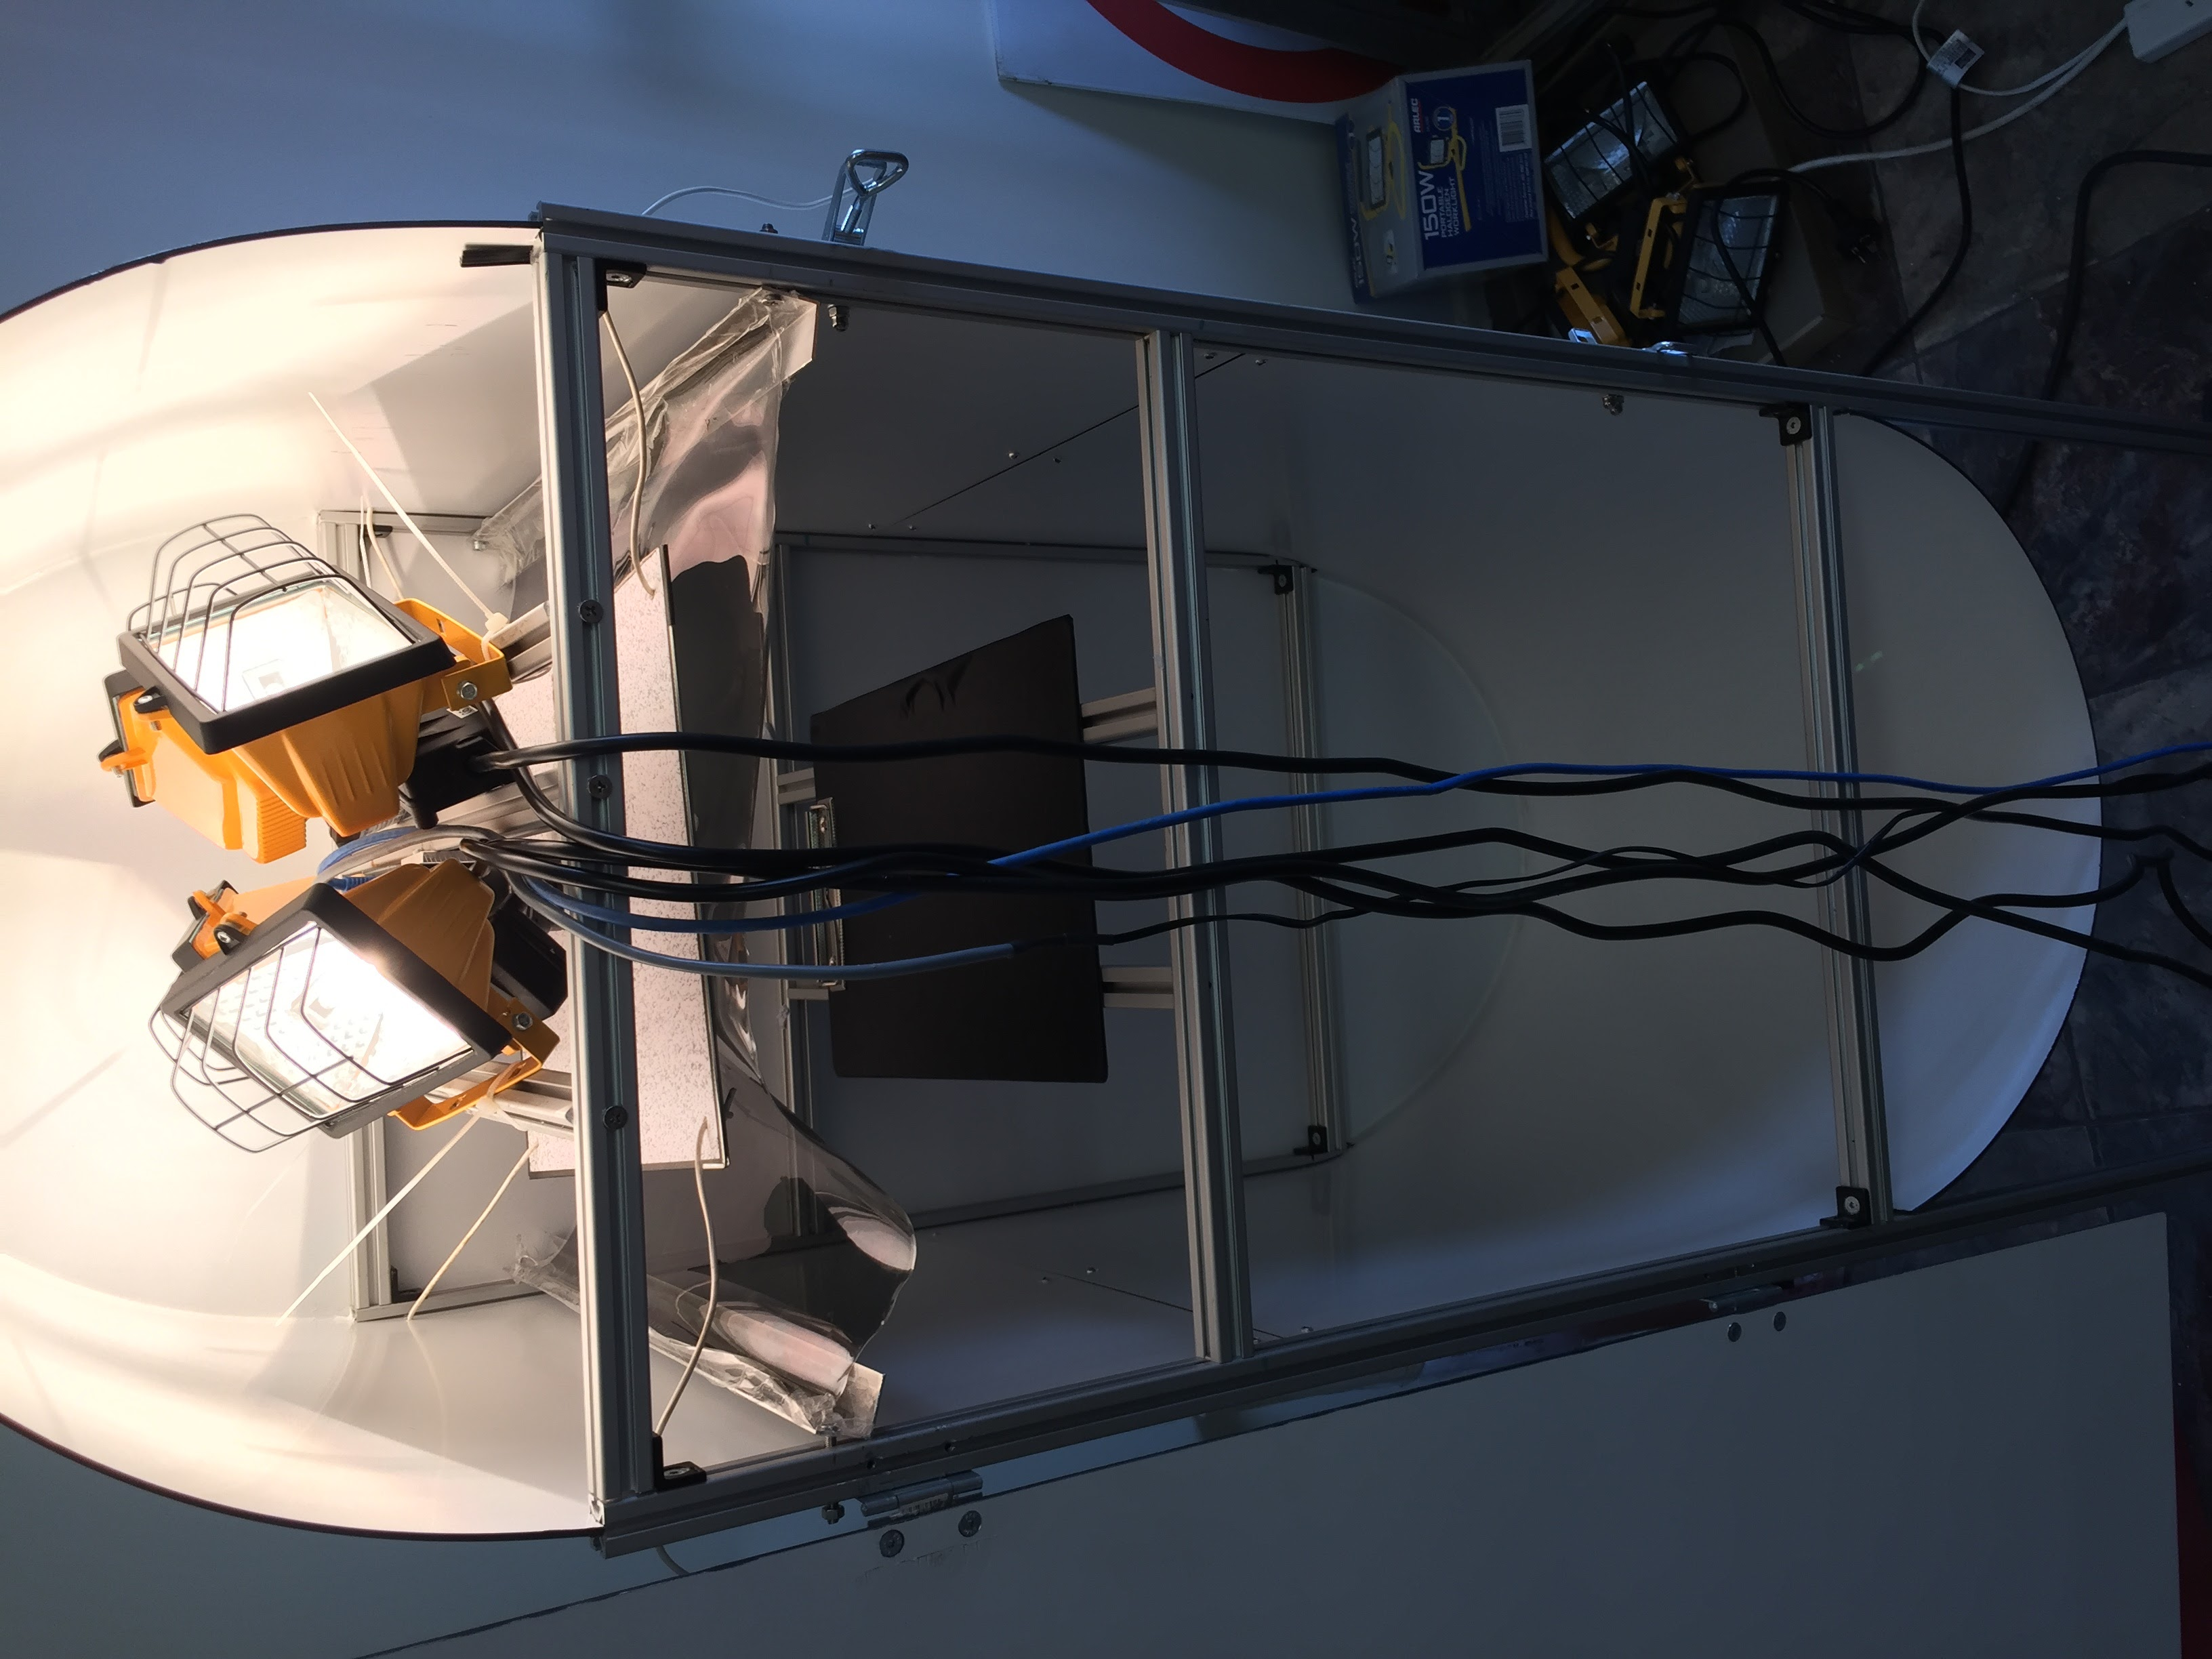
\includegraphics[width=\linewidth,angle=270,origin=c]{bench_hal_film2.jpg}
		\caption{}
		\label{fig:bench_hal_film2}
	\end{subfigure}%
	\caption{Left to right: (a) Halogen work lamps tested facing upwards with a thin film polaroid , and (b) halogen work lamps in a diagonally upward direction with a dark-field blocker.}
	\label{fig:test3}
\end{figure}


LED manufacturing is evolving continuously but has deficits outside the visible spectrum. Infrared LED's are typically either used for devices such as remote control transceiver communication, or night vision cameras, with many different wavelengths in narrow-band selections. As these types of LEDs have manufacturing processes which differ from that of visible (in terms of substrate component material and arrangement), they are specified to have narrow bandwidths of approximately $10nm$, and include centre wavelengths of $780nm$, $810nm$, $840nm$, $890nm$, $920nm$, $940nm$, and $980nm$. However, these devices are not as readily available in a high-power, compact design as is their visible counterparts, rather in small single-diode format making the implementation of an industrial infrared LED system unsuitable. Therefore, the small halogen lamps discussed in chapter \ref{sec:lighting} are used given they can produce the required power with a small footprint and have wide availability. 


Converting the lighting to $12VDC$ power is required in order to provide a more constant current, therefore lighting intensity. An LED's spectral response depends on manufacturer and can range from very poor CRI with 3 distinct bands of R, G, and B (similar to a typical fluorescent lamp), up to $95\%$ CRI that not only emit some IR light, but also render blue colours better than halogen \cite{lumicrest}. However, the IR radiation will cut off around $780nm$ (enough to cover the visible spectrum completely) and therefore will not be suitable for the IR imaging system. $12V$ halogen lamps are commonly used as downlights in residential and industrial applications as they are more efficient, reliable, and the beam is more directional compared to their $240V$ counterpart. Therefore, Automotive LED light bars replaced the halogen work lamps for the visible spectrum, whilst $12V/35W$ halogen lamps provide the IR spectrum. 


\begin{figure}[h]
	\centering
	\begin{subfigure}{0.32\textwidth}
		\centering
		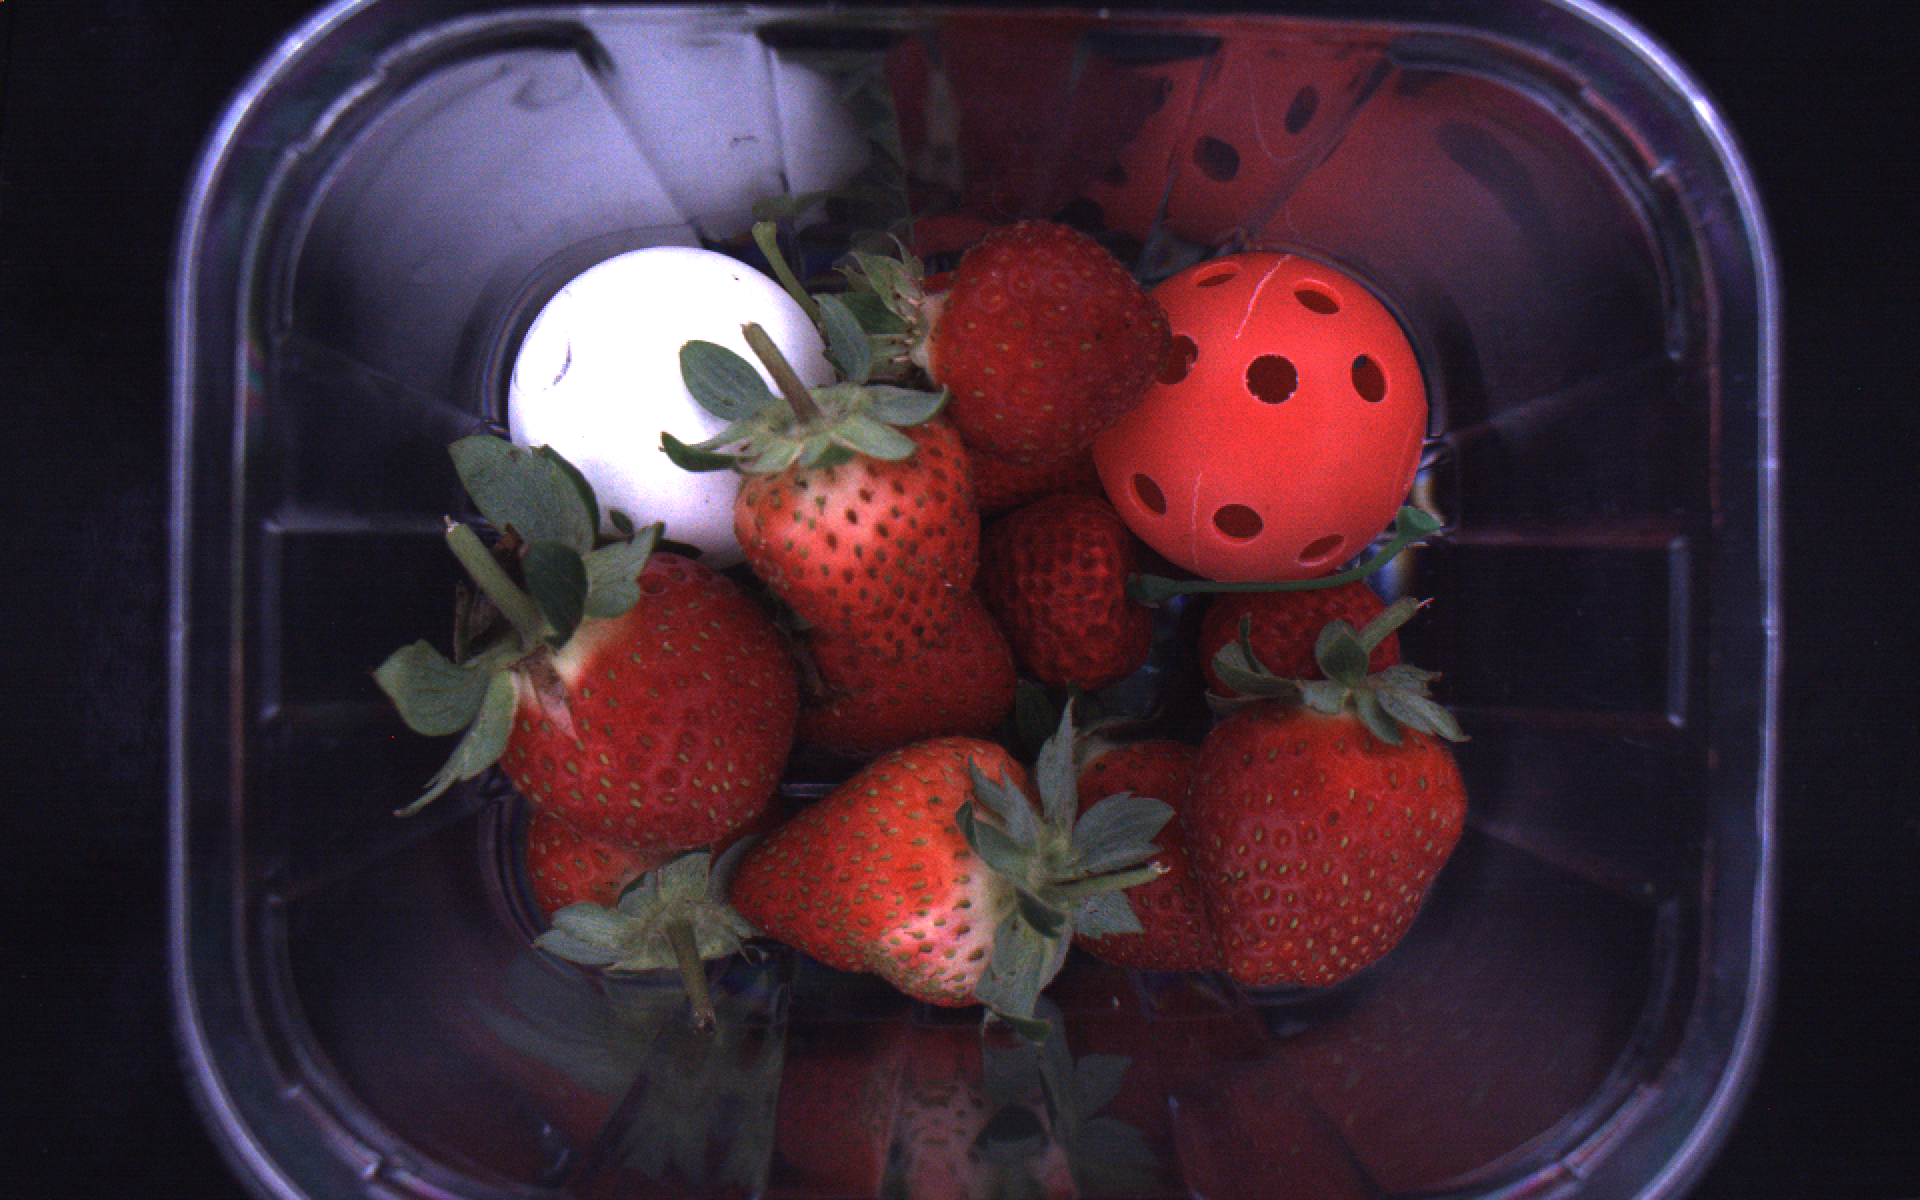
\includegraphics[width=\linewidth]{500us.png}
		\caption{}
		\label{fig:500us}
	\end{subfigure}%
	\begin{subfigure}{.32\textwidth}
		\centering
		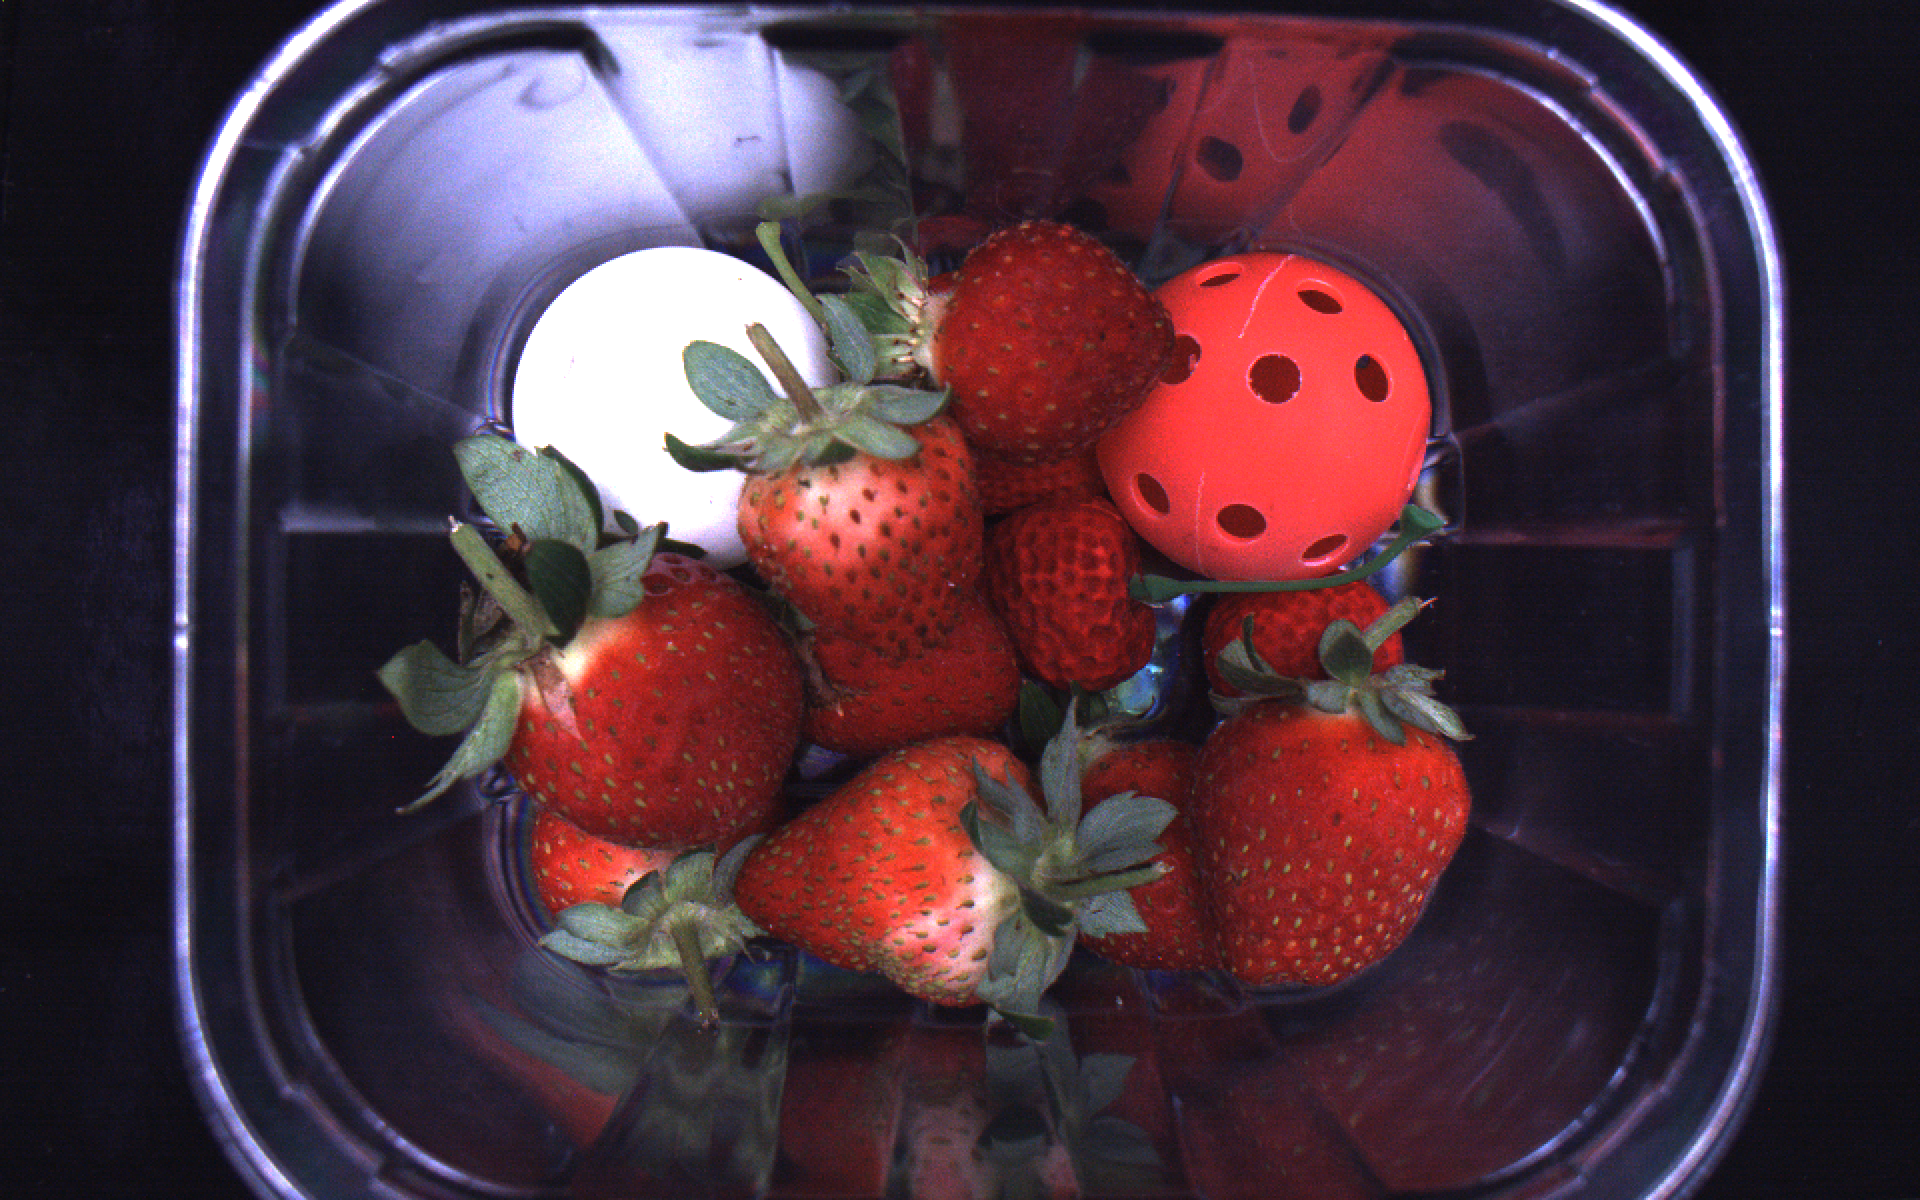
\includegraphics[width=\linewidth]{1ms.png}
		\caption{}
		\label{fig:1ms}
	\end{subfigure}%
	\begin{subfigure}{.32\textwidth}
		\centering
		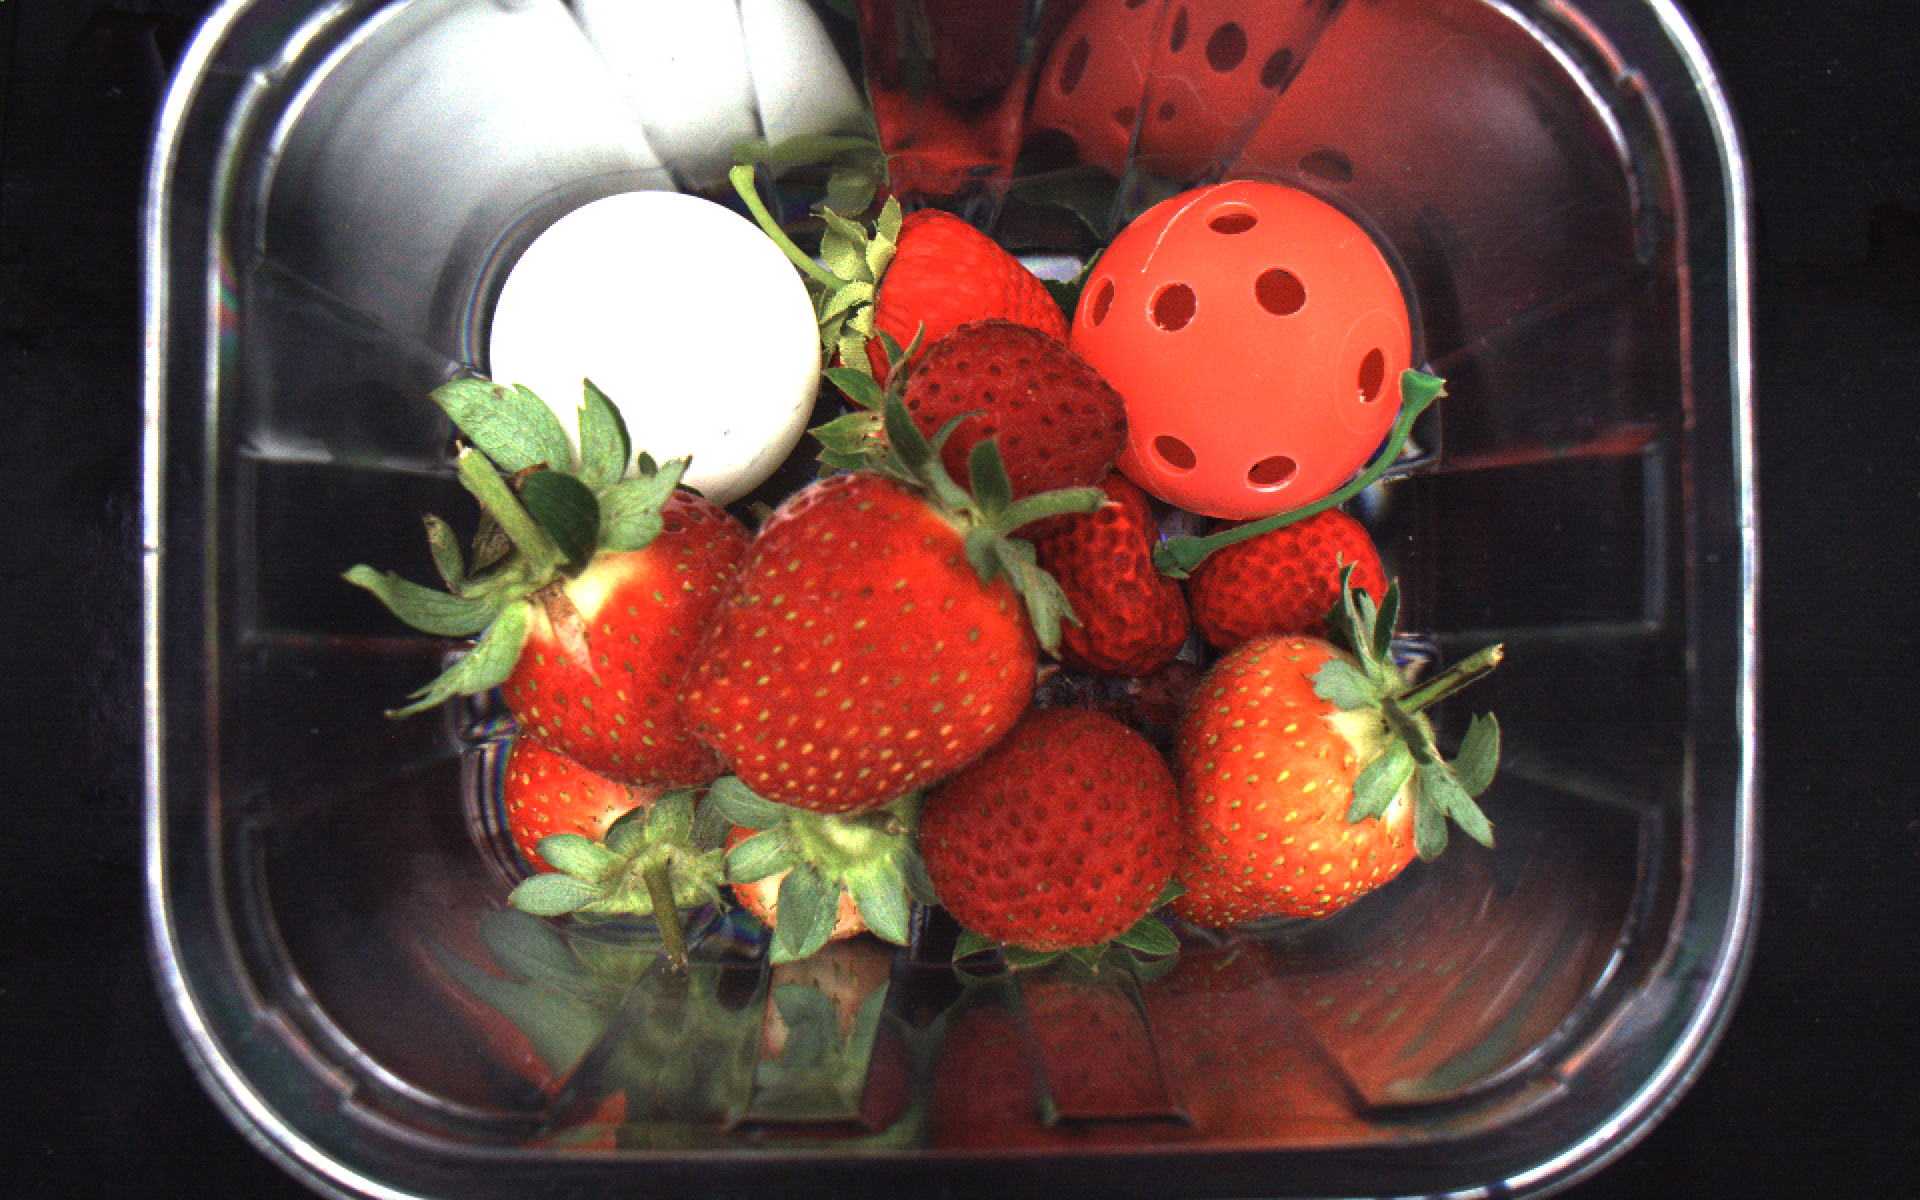
\includegraphics[width=\linewidth]{2ms.png}
		\caption{}
		\label{fig:2ms}
	\end{subfigure}%
	\caption{Images taken using $600W$ of halogen and shutter speeds: (a) $500\mu s$, (b) $1ms$, and (c) $2ms$.}
	\label{}
\end{figure} 

Images captured (Figures \ref{fig:500us}, \ref{fig:1ms}, and \ref{fig:2ms}) using four $150W/240VAC$ halogen lamps with camera shutter speeds of $500\mu s$, $1ms$, and $2ms$, show that the lighting intensity is sufficient for high speed applications. The combined total illumination power consumption (for the top view) is $4\times 150W = 600W$. However, it is well established that halogen lamps are inefficient in regards to lumens per watt ($lm/W$) given they emit much more of the electromagnetic spectrum. White LEDs are manufactured to have much higher efficiency, generating only visible wavelengths. Cheng and Cheng \cite{cheng} found LEDs to be up to $75\%$ more efficient compared to halogen, and Alonzo et al \cite{alonzo} found a $60\%$ improvement which are typical results for these kinds of studies. Therefore, it is estimated that the LED power consumption should be approximately one third that of halogen in order to maintain the same visible illumination. As the number of LEDs can be increased, this is not seen as a limitation of the system, however keeping power, heating, and brightness to a minimum will reduce risk of failure or injury. 


\begin{figure}[h]
	\centering
	\begin{subfigure}{0.5\textwidth}
		\centering
		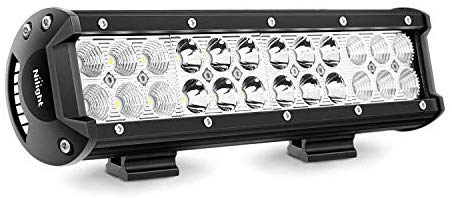
\includegraphics[width=\linewidth]{LED_bar.png}
		\caption{}
		\label{fig:LED_bar}
	\end{subfigure}%
	\begin{subfigure}{.5\textwidth}
		\centering
		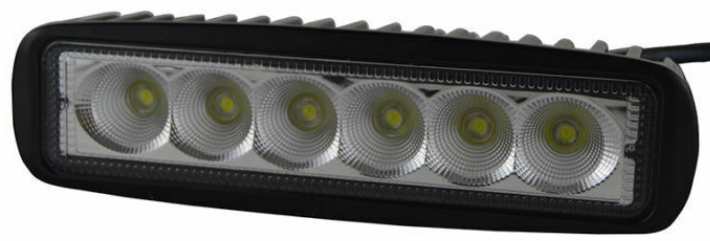
\includegraphics[width=\linewidth]{LED_30w.png}
		\caption{}
		\label{fig:LED_30w}
	\end{subfigure}%
	\caption{(a) Cree\textregistered 72W LED Light Bar, and (b) Cree\textregistered 30W LED Light Bar.}
	\label{}
\end{figure} 

The $72W$ Cree\textregistered LED Light Bars are flood type (an example of the LED bar is shown in Figure \ref{fig:LED_bar}) in order to diffuse, rather than focus the light, to avoid specular reflections. They have a built-in heat-sink as well as high Ingress Protection (IP) rating as they are designed to be fitted externally to off-road vehicles. This gives confidence of consistency and durability in the volatile production environment. Figure \ref{fig:LED_30w} displays the system's midsection LED type which are Cree\textregistered $30W$ LED Light Bar. Using two $72W$ and two $30W$ devices, the total power for each view is $204W$ which is $34\%$ of the halogen lamp power.



\begin{figure}[h]
	\centering
	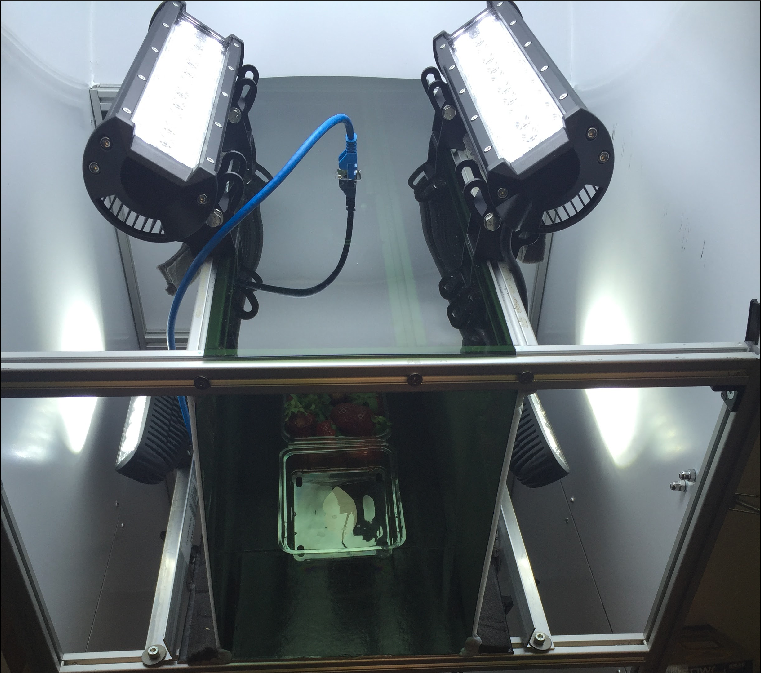
\includegraphics[width=0.7\linewidth]{bench_led_rigid_2.jpg}
	\caption{Installation of LED light bars and rigid polarizing material for the top half of the illumination system.}
	\label{fig:bench_led_rigid}
\end{figure}%

Rigid polaroid sheets eliminate the possibility of light leaking into the acquisition tunnel due there firm shape and size. Thinner polaroids have inconsistent polarisation when warped or bent and can expand with heat over time. Figure \ref{fig:bench_led_rigid} depicts the final configuration of the top half of the system's LEDs and rigid polariser.



\subsection{Machine Vision Camera Protocols}


In terms of functionality and price, there are many variations of machine vision cameras ranging from expensive thermal and NIR, to cheap low resolution monochrome. However, in the visible range where CMOS and CCD sensors are used, the decision for consumers is based on meeting requirements rather than price due to the relatively cheap devices available. This leads to the false assumption that obtaining the highest resolution camera is always the best option, causing potential problems. For example, if the application requires high dynamic range, good contrast at low light, or high quantum efficiency, a camera with increased megapixels may not be the right solution.

Added to functionality, other considerations are that of data transfer, powering, and triggering, or in other words the peripheral connections. If electronic (hardware) triggering is required, an I/O connection port is must be provided additionally to the communication port. Data transfer protocols typically takes one of three variations for high speed applications, namely, 1394IIDC (FireWire\texttrademark), GigEVision\textregistered, and USB3Vision\textregistered. 

1394IIDC protocol has bi-directional data transfer, can be daisy-chained, and can provide power through the connection, but is limited to the bus power of the PCI card. Therefore, applications involving more than two cameras are typically connected in serial and externally powered. Other complexities involve chipset matching and upgrading which can mean computer replacement, and requires at least one PCI card. 

GigEVision\textregistered uses an Ethernet connector which can provide power if a Power-over-Ethernet (PoE) device exists on the host computer. Cable length is an advantage when requiring distances over five meters in length, and four-port PCI cards are common, however they require network communication configurations to set IP addresses and relative ports.

USB3Vision\textregistered offers power over USB, commonly used chipsets, higher throughput, and are less expensive than the previous options. The drawbacks being cable length (less than 5 meters) and IO synchronisation \cite{camera_bus}. Due to the use of external triggering, and the cameras close proximity to the PC, these problems can be negated, therefore selection of this protocol is preferred.




\subsection{Master Processing Computer}

The PC consists of an Azus\textregistered P8Z68 Deluxe Gen3 Motherboard, with a $3.4GHz$ Intel\textregistered Core\texttrademark $i7$ CPU, $8GB$ DDR4 RAM, and a $500GB$ Western Digital\textregistered hard drive. Extra filters added to the PC case prevent excess dust and dirt from prematurely ageing the sensitive electronics or creating failures due to build up. USB3 Gen1 offers $5Gbps$ bandwidth per host controller, however, many USB3 ports, both on motherboard and PCIe additions, share a host controller across up to 8 USB3 ports, reducing the individual throughput of each port. Common uses for USB3 would use only one or two ports at a time where processes are not time critical, additionally if bandwidth limit is reached, the transfer rate will be reduced. However, for the SQA application to run smoothly, a board must be used where each port has it's own dedicated host controller, such as the 4-port Advantech\texttrademark PCI Express x4, 4-Port USB 3.0 Expansion Card. 


\subsection{Control System}
\label{sec:phidget}

Various hardware devices will need to be controllable via the main application, to enable efficient main lighting, signal lighting, peltier, pneumatics, and conveyor control, as well as inputs from some peripheral devices and sensors.


The Phidget\texttrademark is an industrial-style microcontroller with integrated I/O that can be interfaced with a PC and uses screw-clamp electrical connectors. The main advantages of this microcontroller is that it can be programmed in $C\#$ programming language, therefore interfacing with the main application will be simplified, and high power circuit switching when compared to other microcontrollers. The interface board has 16 inputs with $10k\Omega$ input impedance and logic levels either $0V-5V$ or $0V-12V$, as well as 16 relay outputs which can support up to $30VDC$ at $2A$ per channel. 


Given the Lighting must be only turned on when in operational mode, and draws $>2A$ current, the power is switched through a relay bank with the Phidget operating as the controller. This saves energy and lengthens the lifetime of the lighting devices, as well as limiting heat generation.


\begin{wrapfigure}{r}{0.6\textwidth}
	\begin{center}
		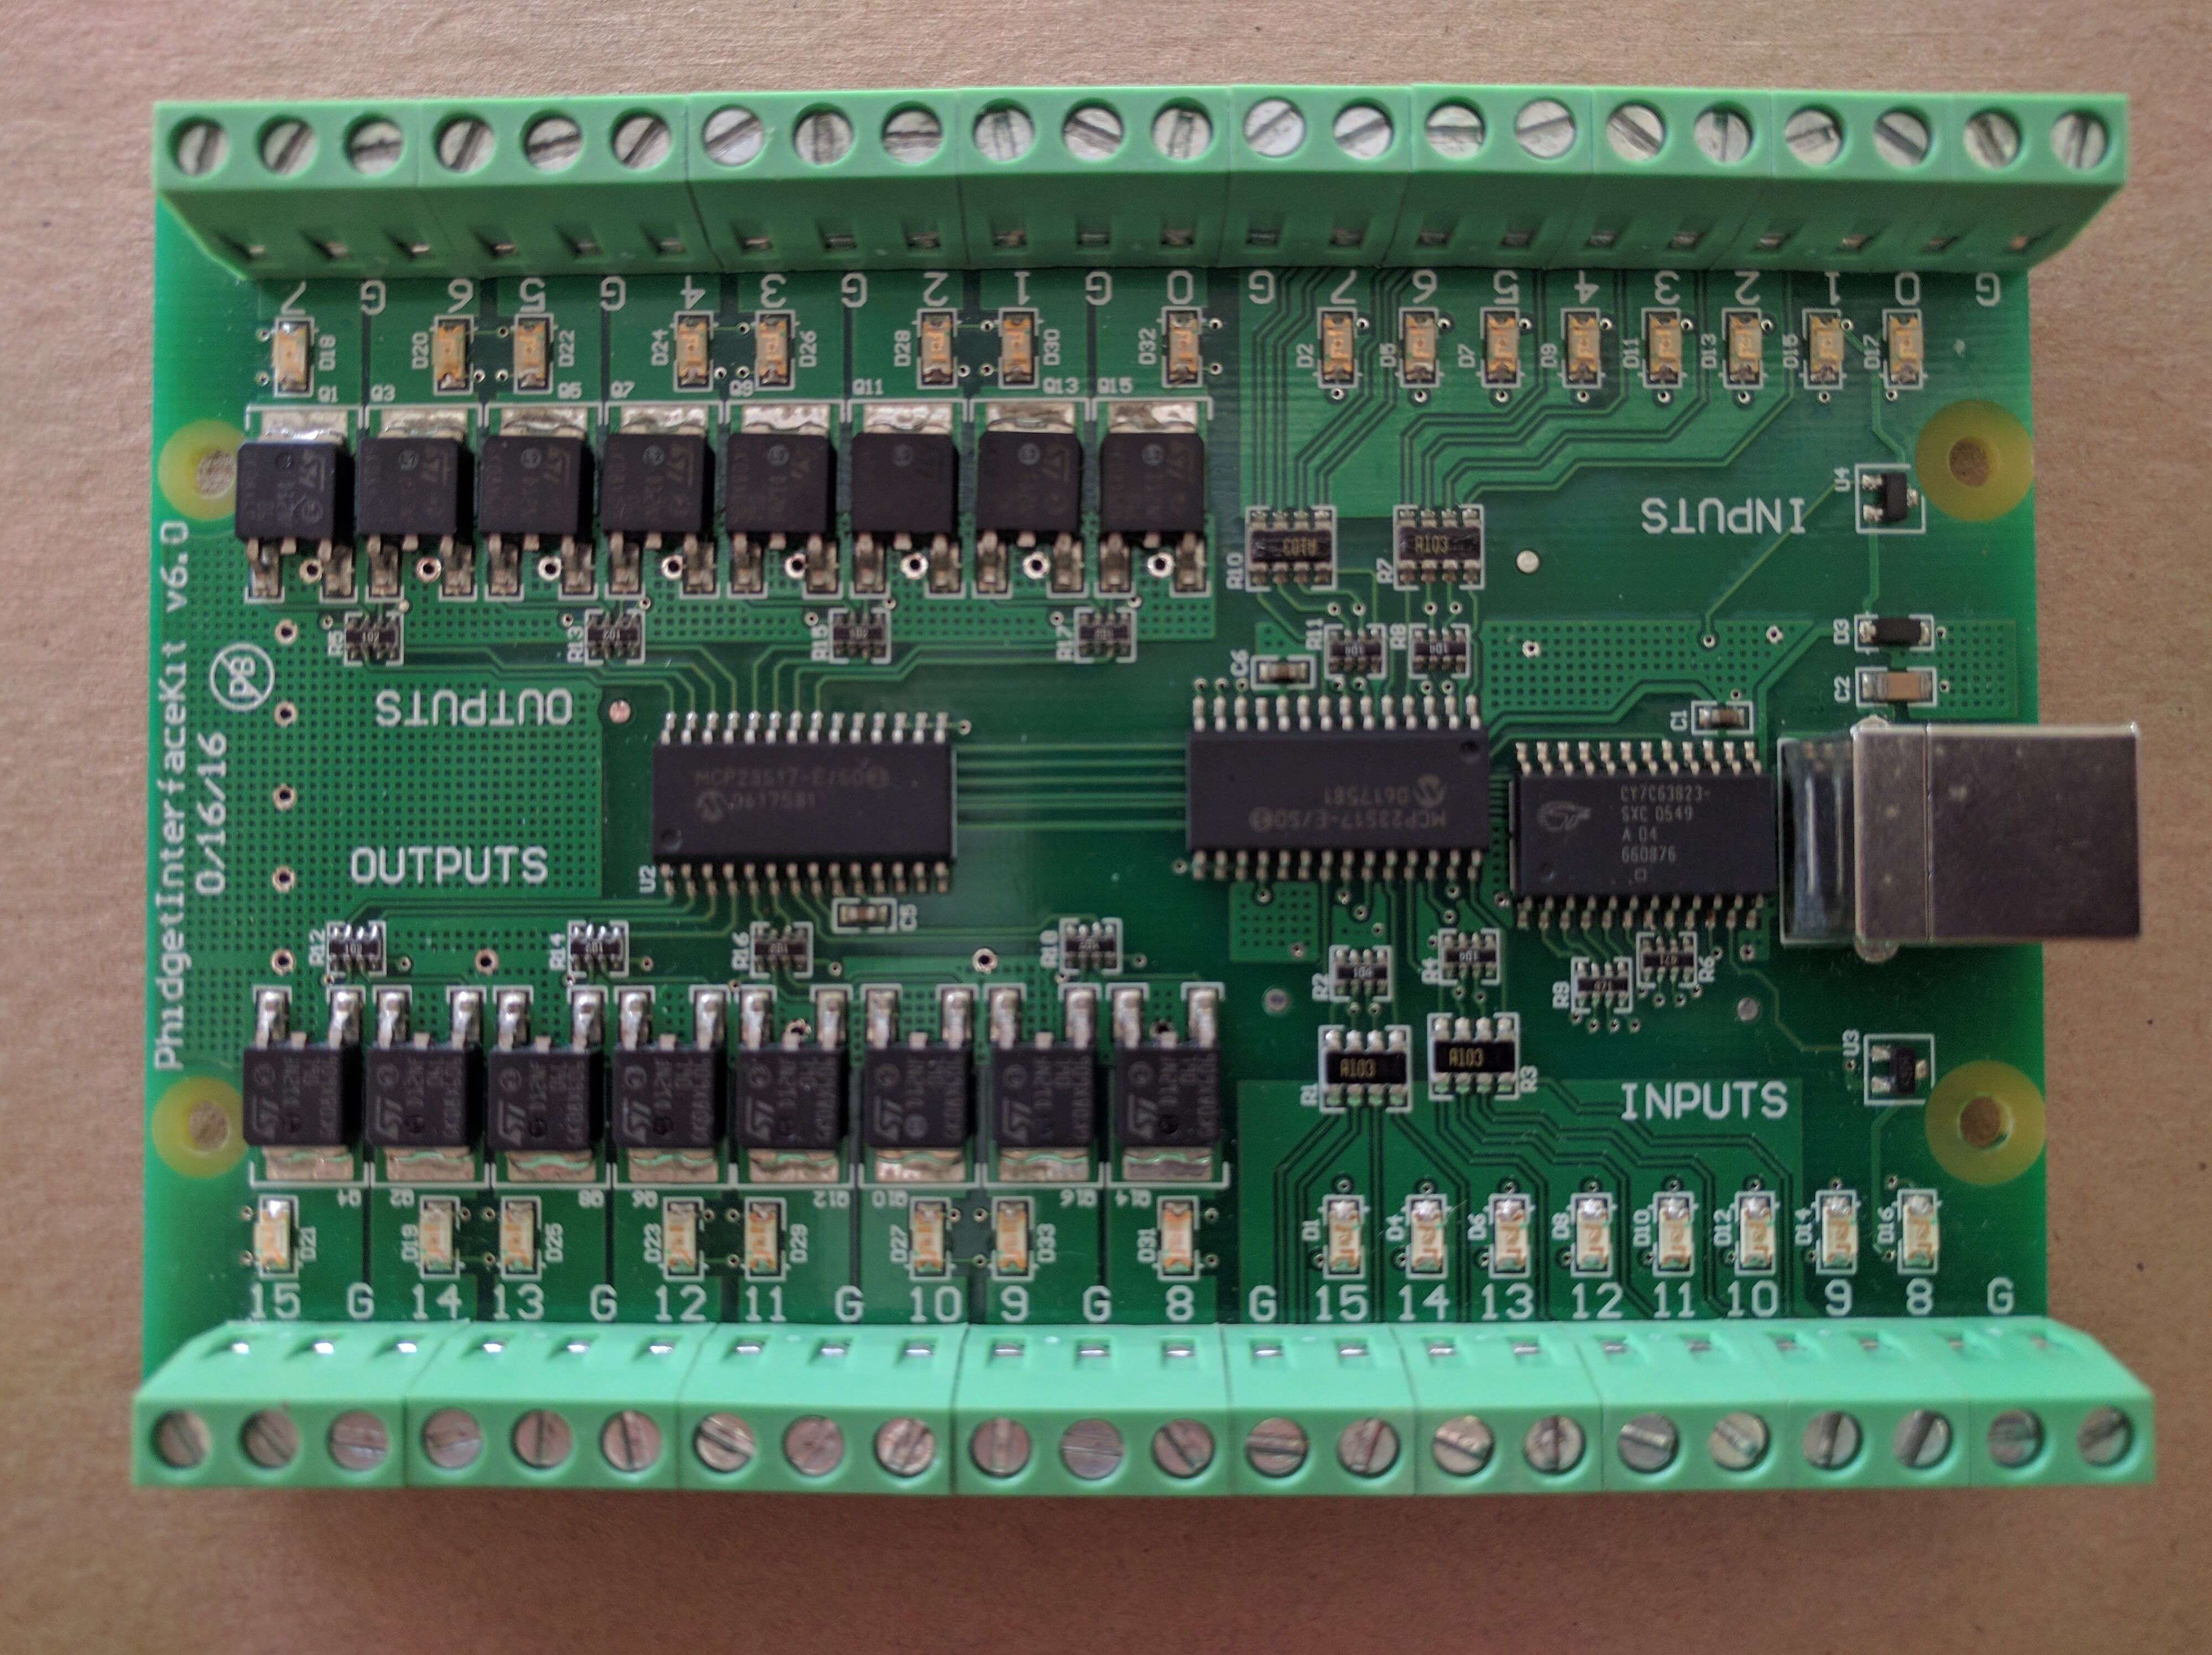
\includegraphics[width=0.6\textwidth]{phidget.jpg}
	\end{center}
	\caption{Image of the Phidget\texttrademark I/O board and the interface connectors on the top and bottom.}
	\label{fig:phidget}
\end{wrapfigure} 


The ejector is a controllable pneumatic system which can release a burst of air on command for a given length of time. The airflow is mechanically adjusted to begin with, then a logic-level $12V$ is applied to engage and disengage the pneumatic actuator. In this way the Phidget can send a signal at the appropriate time, to eject a punnet.


Figure \ref{fig:phidget} shows the screw-clamp I/O connectors on the top and bottom of the image, and the USB connection point for the PC. The Phidget has a $24MHz$ processor, 256 bytes of RAM, and up to $8kB$ of flash storage which makes the device a good option for input/output processes.


The system topology in Figure \ref{fig:overview} describes the control relationship of the PC, microcontroller, relays, PSU and peripheral devices. The PC and PSU are supplied with $240VAC$ power and the PC provides power for the cameras. All other devices (excluding conveyors) are powered by the PSU including the microcontroller, which signals the relay bank to switch the high powered circuits such as LED's, halogen lamps, and pneumatics. 


\begin{figure}[h]
	\centering
	\includegraphics[width=\textwidth]{overview.png}
	\caption{Overview of the electrical connections and control hierarchy of the SQA system.}
	\label{fig:overview}
\end{figure} 

The relays are wired in a normally open configuration so that the relay must be activated (closed) in order to turn on the high powered devices such as lighting. Therefore, malfunctions causing any of the components to fail will result in the system's critical devices to be powered off to prevent the likelihood of damage and waste of power.

\subsection{Software}
\label{sec:software}

Research and experimentation into lighting, polarization, and mechanical construction, was performed in parallel with familiarization and experiments using the software packages provided. HALCON\texttrademark has developed their own language (HDevelop\texttrademark) which has three main points of difference with other languages. Firstly, each variable is categorised as either a \textit{Control Variable} (int, float, tuple, array, etc), or an \textit{Iconic Variable} (image, region, contour, mask, etc) which can be inspected at any point in running, debugging or stepping through a script. Secondly, only discrete operations between control variables can perform the '$:=$' assignment operator due to the design, in which all function arguments contain both input and output (return) variables. For example a function to count regions in an image and paint the number requested, might take the form:

\begin{lstlisting}
num = 3
img = cv2.imread('image.png')
ret_image, count = count_and_find_largest_regions(img, num)
\end{lstlisting} 

would be written in HDevelop\texttrademark as:

\begin{lstlisting}
num := 3
read_image(img, 'image.png')
count_and_find_largest_regions(count, ret_image, num, img)
\end{lstlisting} 

From which point after 'ret\_image' and 'count' will take the values assigned within the function. Each function takes the form:

\begin{lstlisting}
function([, out_c : [, out_i : [, in_c : [, in_i]]]])
\end{lstlisting} 

where lists of  \textit{iconic (i)} and  \textit{control (c)}, can exist or not, for both input and output to the function.


Lastly, HALCON\texttrademark is an interpreted language with the unique property that stores all variables in a database cache as the program runs (in development, using IDE). This means that as each variable is assigned, it is shown in either the \textit{iconic variable} window, or the \textit{control variable} window, giving the user immediate response to code changes and visualisation of the results. This allows for increased efficiency in development of image processing techniques. The screenshot in Figure \ref{fig:halcon_ide} has the IDE split into four windows, displaying the relevant information for agile development.  


\begin{figure}[h]
	\centering
	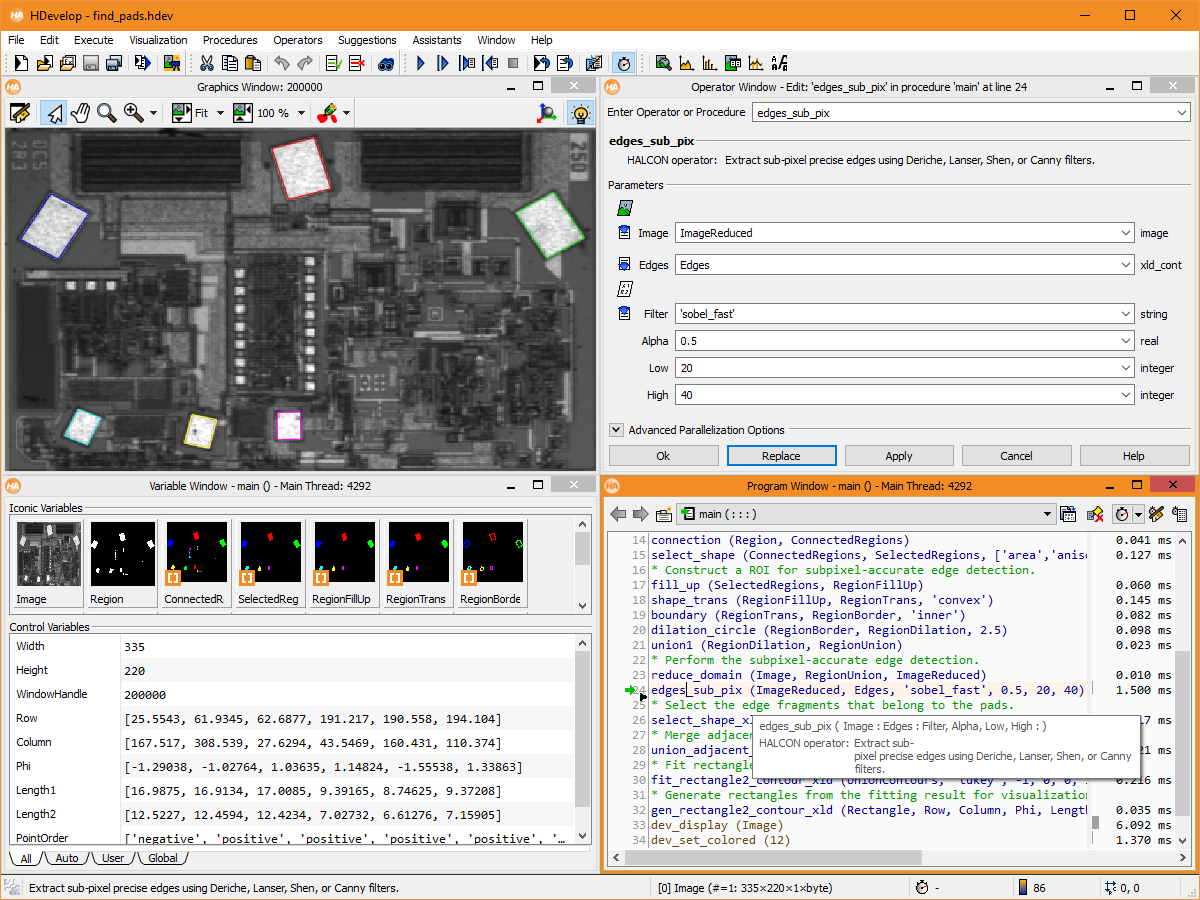
\includegraphics[width=0.9\textwidth]{halcon_ide.png}
	\caption{A screenshot of the HALCON\texttrademark IDE, from left to right, showing the image (Graphics), method (Operator), control/iconic variables (Variable), and script (Program) windows.}
	\label{fig:halcon_ide}
\end{figure} 


There are two methods of integrating HALCON\texttrademark with other applications, given that the programming language HDevelop\texttrademark is not compatible with other languages. An entire script may be inserted in the filesystem, such that it may be called from the main application, after importing the appropriate libraries. This method uses a wrapper function from $C\#$ or $C++$ to call a native HDevelop\texttrademark script as an \textit{External Function Call}. The other method uses the same library to program HDevelop\texttrademark objects in $C\#$ or $C++$ native language. In other words, the operations performed are written locally and natively, using external libraries of objects and operations. HALCON\texttrademark can also convert and export code directly into $C\#$ or $C++$ in order to be used as a dynamic class which would require regular updating, changes or improvements.

Visual Studio\textregistered is a well know development platform whose native programming language is $C\#$, embedded in a rich, professional IDE where creating state-of-the-art apps is common, given the UI development tools (for GUI apps), library linking, debugging tools, git, and deployment features. However, the most important parts of the SQA application, namely the GUI and image processing are supported thus confirming both of these applications suitable for the project.


\subsubsection{User Interface}

The GUI must be simple to use but capable of displaying all the relevant information to inform operators of the status, history, and show images of the punnets being processed. Various controls and indicators are required for both operation and development/debugging such as start/stop buttons, images from all four cameras, camera temperature monitoring, number of punnets assessed, reject information, and sensitivity adjustment. Figure \ref{fig:GUI} presents a screenshot of the GUI after many development iterations and testing. Green bar indicators were added which change colour if either a defect is detected (right hand side indicators), or system status changes such as stop/start, or thread broken (left indicators).  


\begin{figure}[h]
	\centering
	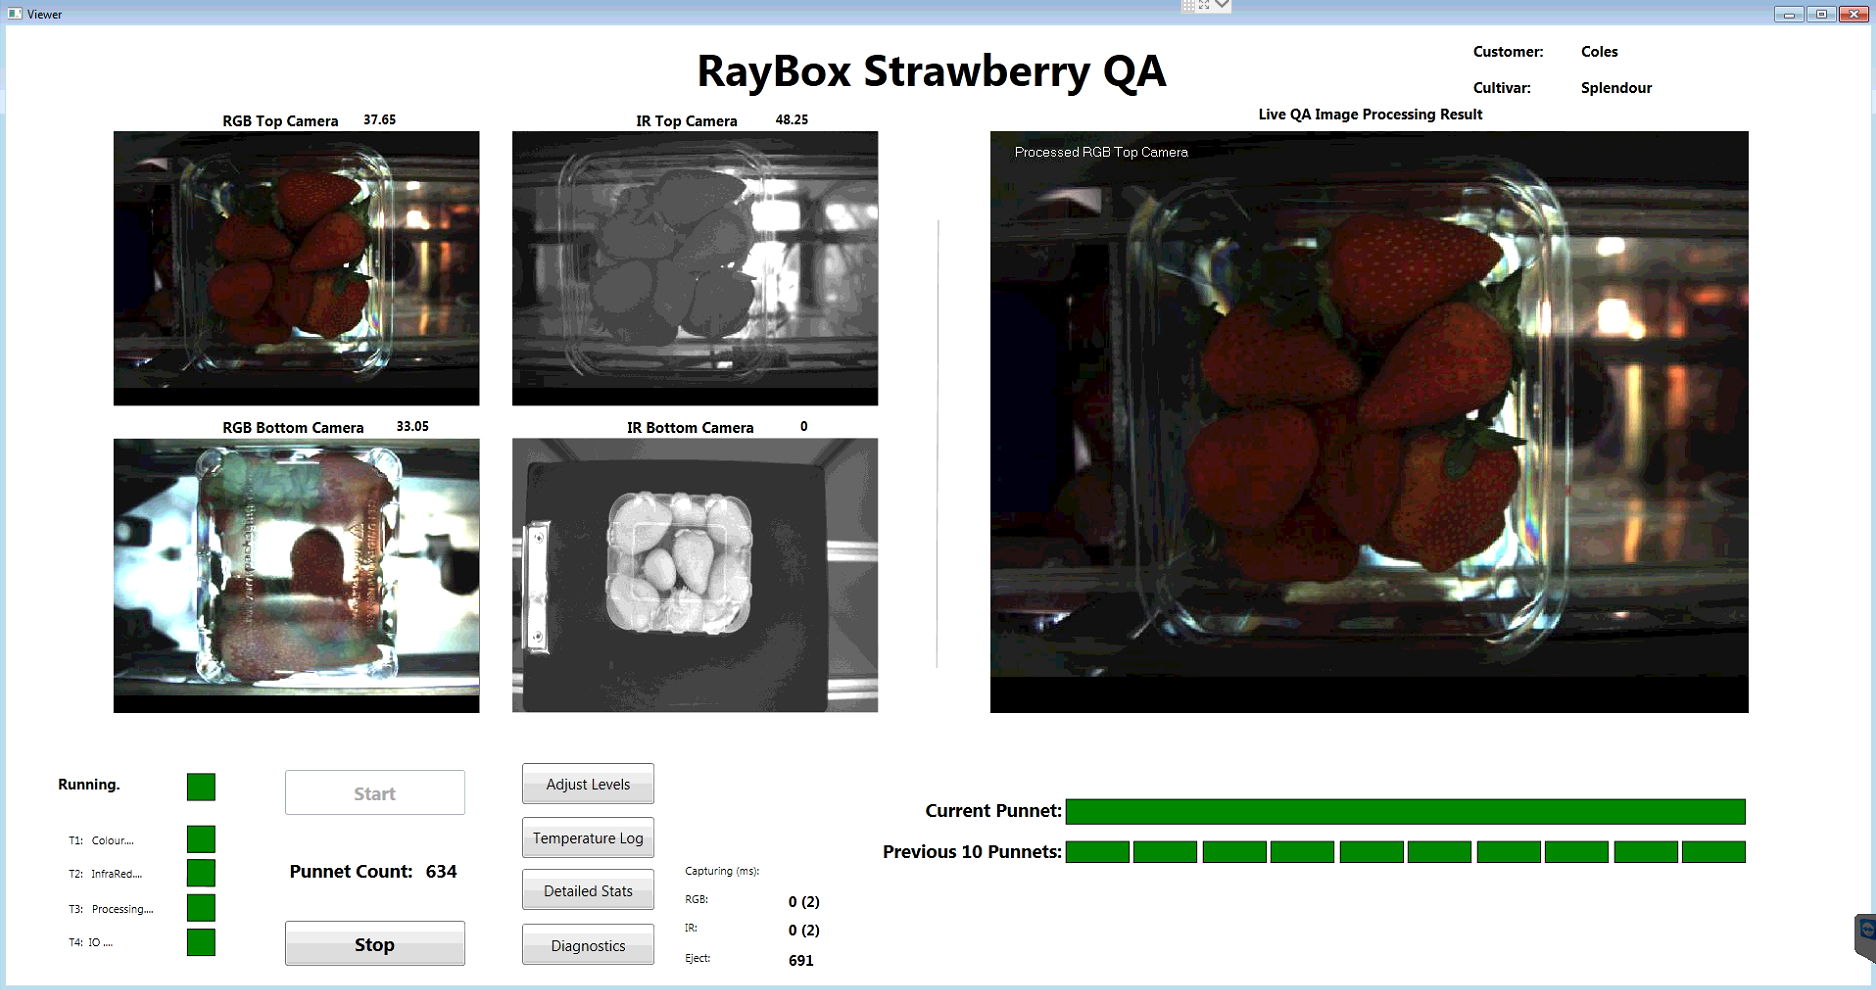
\includegraphics[width=0.8\textwidth]{GUI.png}
	\caption{GUI for the SQA vision system prior to the fourth camera being added.}
	\label{fig:GUI}
\end{figure}
  
  
HALCON\texttrademark's integration capabilities allow the GUI to display a HWindow\texttrademark directly, giving the application the ability to show regions, lines, contours, images, or text generated by the image processing algorithms. 

As HALCON\texttrademark is designed to process images and video streams, it has been developed to include a many camera protocols such as 1394IIDC (FireWire\texttrademark), GigEVision\textregistered, USB3Vision\textregistered, $\mu$eye\texttrademark, including Microsoft\textregistered's DirectShow\textregistered for generic cameras, and support grabbing images from file. For each of the protocols, multiple camera manufacturers (even some camera models) are specifically implemented within the IDE along with a camera connection wizard and code exporter. The wizard allows experimentation with the various controls in GUI style, before exporting the required code to repeat the actions in a new script. 

The application waits until the acquisition sequence is complete before processing and displaying the punnet, therefore updating the GUI at rates up to $2fps$, and might occur whilst images are being captured. This problem is solved with asynchronous threads that can perform acquisition, image processing, I/O, and display separately yet simultaneously.


\subsubsection{Asynchronous Threading}

There are four main tasks required to be performed by the application:


\begin{itemize}
	\item Image Acquisition - Four cameras with external triggers activated at intervals set by the microcontroller.
	\item Image Processing - Analysis of all four images.
	\item Input / Output - Management of signals to and from microcontroller including ejection, errors, and buttons (physical and GUI simulated).
	\item Display - The view is handled by the main thread which spawns the peripheral worker threads.
\end{itemize}


Each of these functions are dependant of each other, but must occur asynchronously. For example, punnet number $n$ may be in the process of analysis (assuming this is the most time consuming thread), whilst punnet number $n+1$ is in acquisition stage. The cameras cannot afford to wait for other processes to complete before acquisition, due to conveyor motion, and must respond immediately. Similarly, the image analysis may require the majority of the $500ms$ window in order to process four images thoroughly. Furthermore, the image processing cannot occur without complete acquisition (all four images), likewise the GUI cannot display, or IO eject, without being processed. This means signalling semaphores must be used to send messages between threads and allow each process to know the application state at all times.

\begin{figure}[ht]
	\centering
	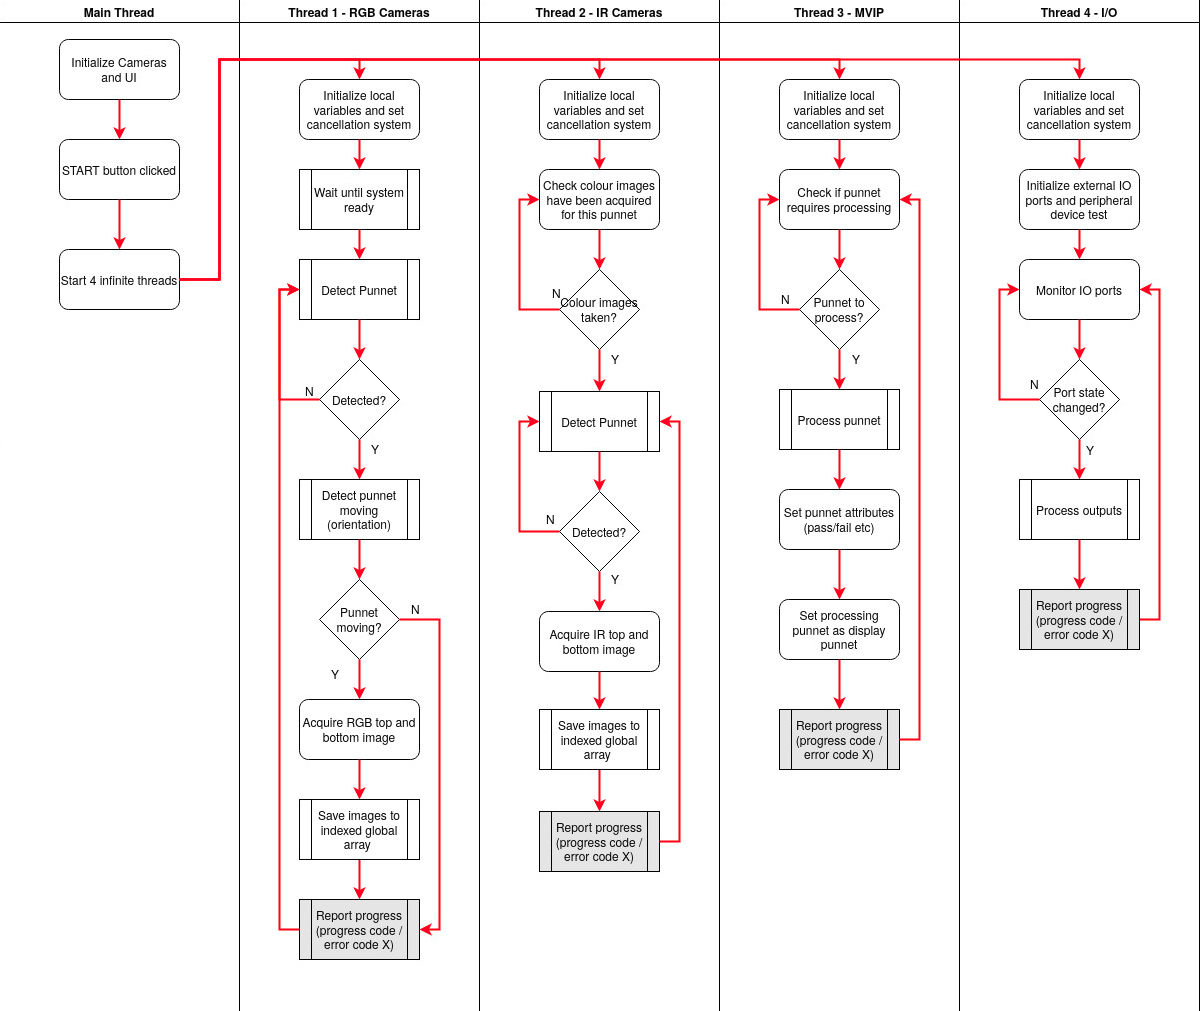
\includegraphics[width=0.95\textwidth]{software_flow_1.png}
	\caption{Flow chart of the main application with each of the five threads (including main).}
	\label{fig:software_flow_1}
\end{figure} 


The lighting enclosure is designed with visible RGB on one end and halogen IR on the opposite end (in the direction of punnet flow). In order to maximise lighting at the correct spectral wavelengths, at the optimal time, the RGB and IR cameras are separated to be centred in the respective lighting environments. Taking this into consideration, a fifth thread was added to monitor the RGB and IR camera triggers separately. Figure \ref{fig:software_flow_1} illustrates the flow of each thread along with it's \textit{progress reporting} action shown in Figure \ref{fig:software_flow_2}. A $C\#$ thread can report it's progress at some time during the threaded procedure by using a protected method (semaphore / mutex) to share information outside its scope. 

\begin{figure}[ht]
	\centering
	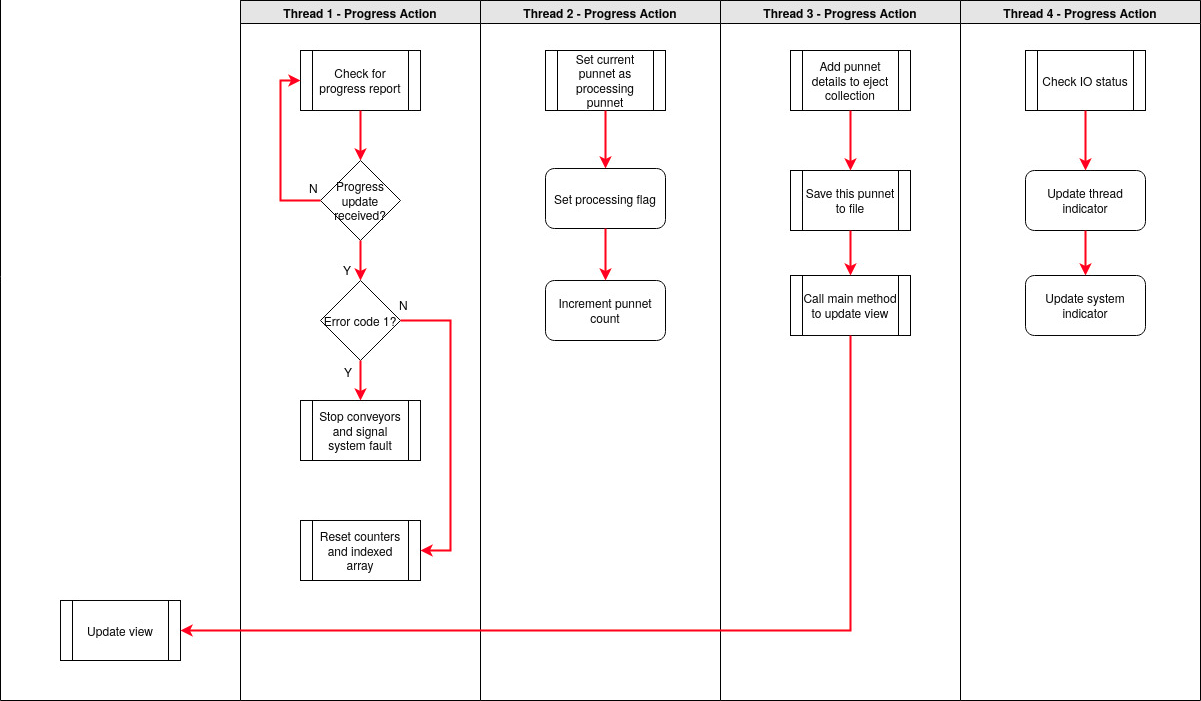
\includegraphics[width=0.95\textwidth]{software_flow_2.png}
	\caption{Flow chart of the progress reporting which occurs after each thread cycle.}
	\label{fig:software_flow_2}
\end{figure} 

Firstly, the main thread spawns four worker threads; one for each set of cameras, one for image processing, and one to monitor I/O. The RGB thread waits for the image to begin being buffered by the cameras (triggered by the sensor) before beginning the process of image collection and confirmation. The IR thread waits for the confirmation (semaphore) that the first images have been acquired, before beginning a similar process to receive and populate the remaining images for the current punnet. Once the all images are acquired, another semaphore is used to signal the image processing thread to begin. Each of these processes returns to wait for semaphores each iteration which also greatly helps in the synchronisation of punnet images. The last thread continually interrogates each of the I/O components by way of polling, using the Phidget\texttrademark's API. The hardware and software is designed to create an interrupt event if any of the input ports change state. Therefore, methods to handle each state change (low-->high and high-->low) for each input is required. The inputs are polled once every 200ms in order to give a response from the system in a timely manner, both for safety and operator usability.

The progress reporting for the RGB thread performs camera/image error checking, and signals the IR thread, whose progress confirms image count and assigns a punnet number, before signalling the image processing thread to begin. The image processing thread finalises the results and signals the main thread to display, whilst the I/O thread reports nothing until a state is changed, at which time the main thread is notified.


The RGB and IR threads are not dependant or in scope of each other, however, they need to synchronise in order to match the two sets of images. This was achieved by using an array of 10 \textit{punnet} objects which were constantly cycled and reused within the application (as no more than 5-6 punnets can occupy the space between the cameras and the ejector). Using this method, simple logic could be used in order to confirm the punnet count matched before populating the object. 



\subsubsection{Image Processing}

The image processing component is performed in  HALCON\texttrademark V-11.0 which is an industry standard image processing tool developed by MVTec Software GmbH\texttrademark. As described earlier in this chapter, HALCON\texttrademark is designed for development efficiency and rapid deployment. Consequently, a simple colour algorithm was developed in order to extract under ripe pixels in the fruit. Firstly, the RGB image is transformed into HSV colour space (HSV properties shown in Figure \ref{fig:hue_sat}), to allow detection of the berry regions, and their ripeness. The saturation channel provides very good background segmentation given it's property that saturated pixels (black or white pixels) occupy one end of the values, and unsaturated (vibrant colour) occupy the other. This means the red strawberries can be extracted by means thresholding and morphology with a very accurate boundary around the berry flesh even with the occluded nature of the randomised packing (Figures \ref{fig:bg_example} and \ref{fig:sat_thresh}).


\begin{figure}[ht]
	\centering
	\begin{subfigure}{.4\textwidth}
		\centering
		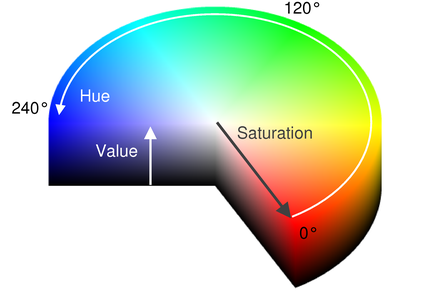
\includegraphics[width=.9\linewidth]{hue_sat.png}
		\caption{}
		\label{fig:hue_sat}
	\end{subfigure}%
	\begin{subfigure}{.4\textwidth}
		\centering
		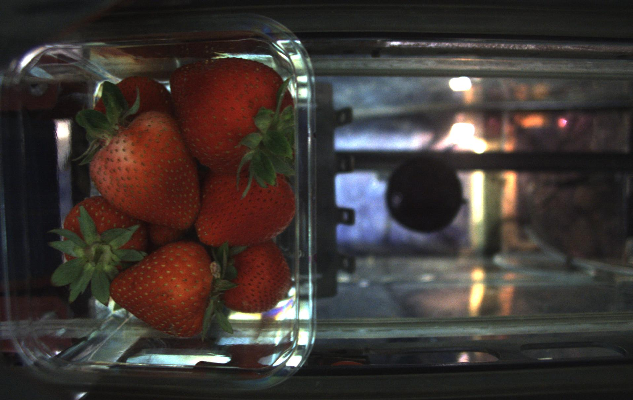
\includegraphics[width=.9\linewidth]{bg_example.png}
		\caption{}
		\label{fig:bg_example}
	\end{subfigure}%
	
	\begin{subfigure}{.4\textwidth}
		\centering
		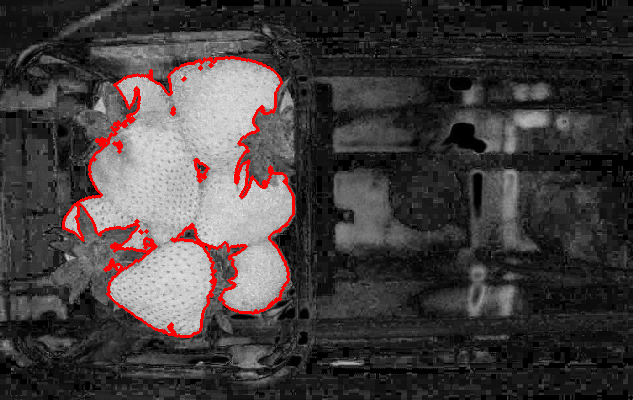
\includegraphics[width=.9\linewidth]{sat_thresh.png}
		\caption{}
		\label{fig:sat_thresh}
	\end{subfigure}%
	\begin{subfigure}{.4\textwidth}
		\centering
		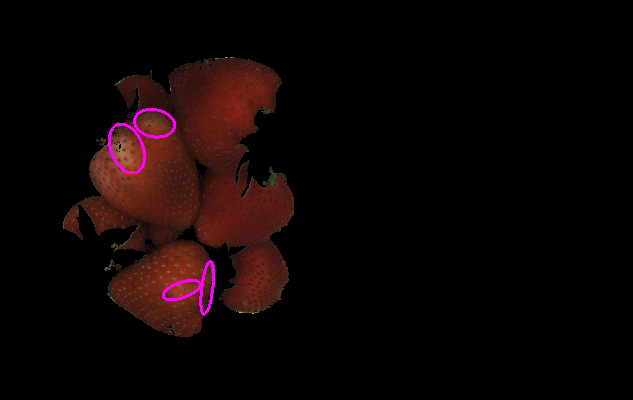
\includegraphics[width=.9\linewidth]{hue_processed.png}
		\caption{}
		\label{fig:hue_processed}
	\end{subfigure}%
	
	\caption{Left to right: (a) HSV colour space showing hue circle and saturation vector, (b) raw RGB image with some background lighting noise, (c) saturation channel with berries segmented after pre-processing, (d) image reduced to berry region showing four small under ripe areas detected by the algorithm.}
	\label{}
\end{figure}


To calculate HSV colour space given three channels R, G, B and $Min = min(R, G, B)$, $Max = max(R, G, B)$:
\begin{equation}
	V = Max
\end{equation}
\begin{equation}
	S = 
	\begin{cases} 
		0, & Max=Min \\   
		(Max-Min)/Max, & otherwise        
	\end{cases}
\end{equation}
\begin{equation}
H = 
\begin{cases} 
rad(60) \cdot ((G-B)/(Max-Min)), & R=Max \\
rad(60) \cdot (2 + (B-R)/(Max-Min)), & G=Max \\
rad(60) \cdot (4 + (R-G)/(Max-Min)), & B=Max \\   
\end{cases}
\end{equation}



The following operation is performed on each S-channel pixel $S[x,y]$ to find the region $R_{berry}$:
\begin{equation}
R_{berry} = \sum_{n=1}^{P} 128 \leq S[x,y]_n \leq 255
\end{equation}

where $P$ denotes the total number of pixels. 



This is then followed by colour analysis of the hue channel in order to quantify the amount of pixels which lie outside the range $10<H<48$ where H is the hue circle from $0^{\circ}-360^{\circ}$. If we take $D$ as degrees of the hue circle, then the equation for $\alpha$, the corresponding grey-value is calculated as:
\begin{equation}
\alpha = round\Big\{255\cdot \frac{D}{360}\Big\}
\end{equation}


These values can be inserted to the equation and performing the operation on the H channel, the region $R_{colour}$ can be extracted in as follows:
\begin{equation}
R_{colour} = \bigg\{\sum_{n=1}^{P} \alpha_1 \leq H[x,y]_n \leq \alpha_2\bigg\} \in R_{berry}
\end{equation}


where $\alpha_1$ and $\alpha_2$ are the grey level upper and lower limits to threshold. For red strawberries the initial values are set to $0^{\circ}$ and $20^{\circ}$ which equates to 0 and 14 for $\alpha_1$ and $\alpha_2$ respectively.

Pre-processing consists of reducing the image to a Region Of Interest (ROI) in the spacial location where the punnet is consistently captured. The post-processing methods use morphology, removal of small regions (noise reduction), and area calculations to return the affected areas as indicated by the ellipses in Figure \ref{fig:hue_processed}.


As the saturation channel extracts all of the berry flesh whose colour is saturated, only the darkest parts of the berry flesh will be excluded. However, when extracting colour ranges using the hue channel, darker regions can be falsely classified. Shadowed areas and berry occlusions generate high false positives in the case of over ripe analysis due to the crossover between over ripe flesh and occluded sound material. This problem will need to be addressed in order to provide accurate grading of over ripe berries. 


\section{Project Contributions}


\subsection{Enclosure Construction}

The prototype frame is built from robust aluminium material commonly applied to structural elements for many applications. The frame has T-slot groves along the length of each side of each bar, and can be cut and fit together to form almost any shape required. These highly configurable components are utilised in order to experiment and optimise the various positional variations of several items such as lighting, cameras, conveyors, punnet orientation, polariser angle, and placement of motors. 

Using stainless steel sheets as cladding in order to enclose the internal components, the external AC lighting is sufficiently blocked from interfering with the acquisition and analysis of images.   



\subsection{Power Systems}
\label{sec:electronic_power}

The electronics and power supply will accompany the enclosure to the production floor given that DC power is required to avoid flickering. Furthermore, the control system microprocessor, fuses, wires and relays need to be installed in order to operate the various controls. As the vision enclosure does not allow for power supply storage or peripherals inside, an electronic component box is used to contain the above-mentioned items. 

Safety is of great concern given that any packing floor operator may come into contact with the system. Therefore, the design must address critical safety hazards such as electrocution, shock, arcs or short circuits (potentially causing fire) and eye damage from intense lighting. Fuses are added to the high current wiring delivering power to the main consumption devices (and to some lower powered devices) which will break the circuit on overload. Normally open wiring for relays are used to switch high power circuits, given they will also break the circuit on overload or malfunction.  


All electronic requirements are as follows:

\begin{itemize}
	\item PC for image processing and control of devices and hardware
	\item Uninterruptible Power Supply (UPS) for PC continuity
	\item 2 x $240V$ conveyor motors
	\item Lighting for illumination
	\item Cameras
	\item Peltier devices and fans 
	\item Punnet sensors
	\item Microcontroller for hardware operation
	\item Relay bank to switch high-power sources
	\item Intake/exhaust/cooling fans
\end{itemize} 

The first three items require AC mains power ($240V$) and can therefore be addressed by using readily available extension leads and a power board. The remaining items use DC power have been quantified in order to design the power supply system.

A small power supply was used to power the prototype, which at this stage, only included the top illumination cluster. The $12V/5A$ power supply was only able to power either the LEDs or halogens for testing purposes, and not both at once due to the current limitation, indicating that a more powerful source was required. As the enclosure will ultimately be positioned on the production floor, the electronics must accompany the vision system, and provide a substantial amount of DC power. 

Industrial power supplies can be expensive, have long lead-times (for initial construction and replacements), and may not have internal protections (such as short-circuit, over-current, thermal) and multiple outputs. However, a high-end gaming PSU can provide these features including automatic fault detection and shut-off, multiple $12V$ outputs (can be configured due to the wiring loom containing several high current wires), and greatly beneficial $5V$ and $3.3V$ outputs of lower current, which can be used to power logic circuits. The lighting must be powered by DC in order to prevent capturing the changing intensity of an alternating current AC. In order to provide enough power to the system, a 1200W PSU was retrofitted to handle the relevant lighting, controls, sensors, and microcontroller power. Various safety systems built into the gaming power supply provide protection against over current, over voltage, overheating, and short circuit, making it an ideal $12V$ power supply to be used for the lighting and peripheral devices, and can satisfy the total power requirements.

\begin{table}[h]
	\centering
	\caption{Table of DC power requirements used in the SQA vision system.}
	\label{tab:DC_power_table}
	\begin{tabular}{lccccc}
		
		\toprule
		\textbf{Element} & \textbf{Volts ($V$)} & \textbf{Current ($A$)} & \textbf{Power ($W$)} & \textbf{No.} & \textbf{Total ($W$)}\\[8pt]
		\midrule
		
		Exhaust Fan & 5 & 0.1 & 0.5 & 1 & 0.5 \\[4pt]
		\midrule
		Phidget Logic Power  & 5 & 0.1 & 0.5 & 1 & 0.5 \\[4pt]
		\midrule
		Peltier & 5 & 1.5 & 7.5 & 4 & 30 \\[4pt]
		\midrule
		Peltier Fan & 12 & 0.1 & 1.2 & 4 & 4.8 \\[4pt]
		\midrule
		Phidget Supply Power & 12 & 1 & 12 & 1 & 12 \\[4pt]
		\midrule
		LED Light Bar - $72W$ & 12 & 6 & 72 & 4 & 288 \\[4pt]
		\midrule
		Halogen - $35W$ & 12 & 2.9 & 23.3 & 8 & 280 \\[4pt]
		\midrule
		LED Light Bar - $30W$ & 12 & 2.5 & 30 & 4 & 120 \\[4pt]
		\midrule
		Photoelectric Sensors & 12 & 0.1 & 1.2 & 4 & 4.8 \\[4pt]
		\midrule
		Pneumatics & 12 & 0.3 & 3.6 & 1 & 3.6 \\[4pt]
		\midrule
		Traffic Lights & 12 & 0.3 & 3.6 & 1 & 3.6 \\[4pt]
		
		\midrule\midrule
		\textbf{Total } &  &  &  &  & \textbf{747.8}\\[8pt]
		\bottomrule
		
	\end{tabular}
\end{table}



A Cougar\texttrademark $1200W$ gaming PSU is used for the DC power requirements with 2 x $12V$ high power rails at $100A$ maximum current in total. It also supplies 4 x $5V$ and 2x $3.3V$ lines, and a low power $-12V$ line giving the advantage of supplying up to $24V$ with low current. All of these outputs can also be fused using automotive in-line fuses, protecting each DC circuit. The breakdown in Table \ref{tab:DC_power_table} accounts for $~750W$ of device power consumption leaving $450W$ headroom for safe operation and allowing additional devices if required at a later stage.


The PSU is designed specifically to connect to a PC motherboard and its peripherals such as hard drives, fans, and graphics / PCI expansion cards using unique connectors which only allow certain devices to plug into each. As the vision system does not require these connectors, the power distribution is concentrated into its two $12V$ rails, rather than the default - multiple, medium power lines distributed to many devices. A damage prevention safety measure employed by many PSU manufacturers requires units to have a load attached in order to prevent accidental powering whilst partially or not connected. This is addressed by adding a high power, small resistor ($1W/10\Omega$) across the load detector circuit.  


Each $12V$ power line is merged into one of two fused distribution boards with respective ground lines connected to one of the two brass grounding bar. Both the distribution box and ground bar are rated for $100A$, with current being drawn as required up to the fused limit for each circuit. That is, any of the outputs can be used for high or low powered devices as long as the appropriate fuse is used, and the total current requirement for all devices does not exceed $100A$. 



\subsection{Lighting and Polarisation}


Cross-polarisation has been successful in removing the many specular reflections strawberries produce due to their two-dimensional curved surface and seed craters. Removing these specularities requires two orthogonal polaroids where the angle of polarisation for each is $90^{\circ}$ apart. However, this reduces lighting considerably, meaning that more powerful lighting is required to gain the same level of illumination with the same shutter speed and aperture.


\begin{table}[h]
	
	\caption{Lighting configurations used during lighting experiments. (1) $0^{\circ}$ downward in the same direction as camera, (2) 
		$45^{\circ}$, and (3) $90^{\circ}$ in relation to the camera, respectively.}
	\label{tab:lighting_orientation}
	\begin{tabular}{c*3{I}}
		\centering
		No. & Configuration & Single Polariser & Cross Polariser \\
		
		1 &
		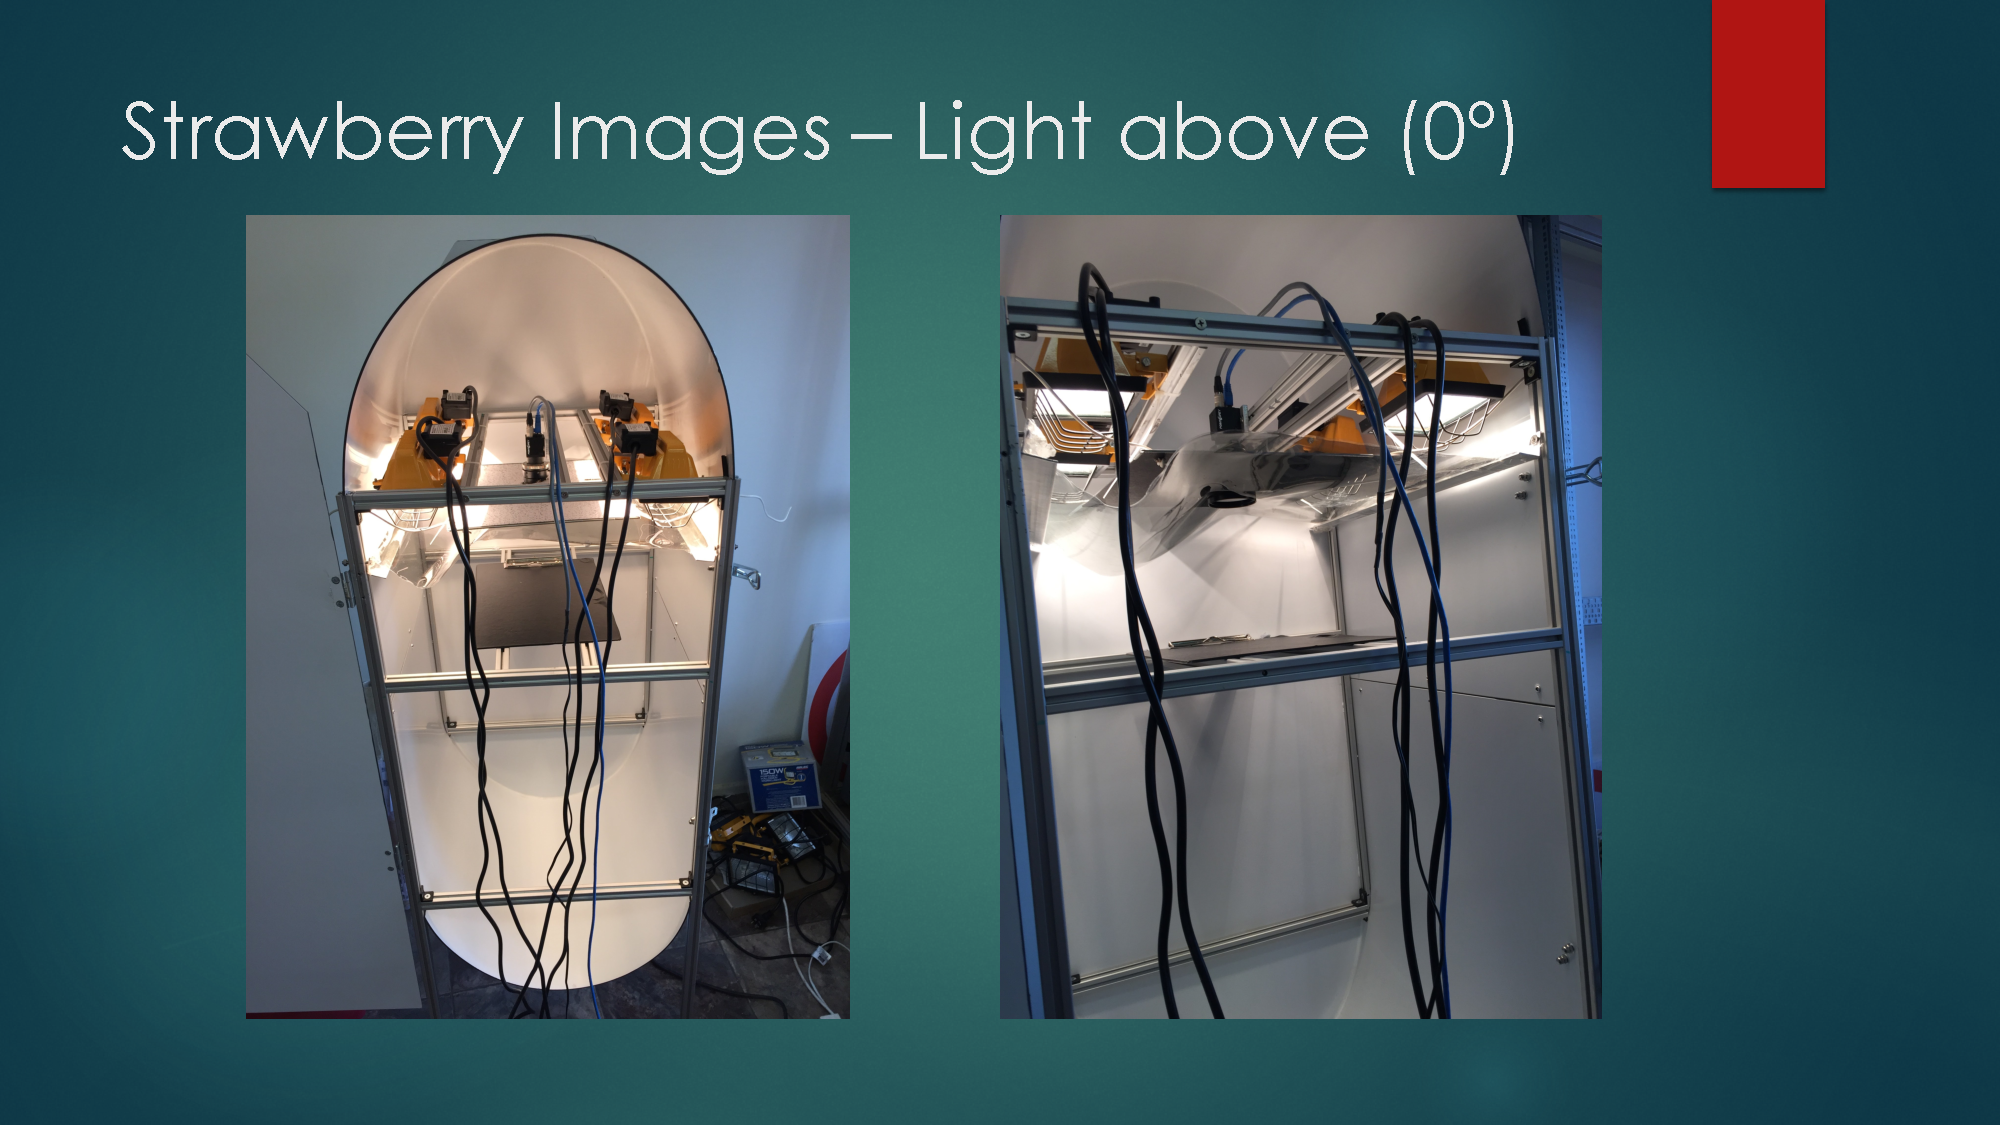
\includegraphics[width=\linewidth]{images/lighting_angle/0/0_degrees_setup.pdf} & \includegraphics[width=\linewidth]{images/lighting_angle/0/0_deg_polar.jpg} & \includegraphics[width=\linewidth]{images/lighting_angle/0/0_deg_cross_polar.jpg} \\
		
		2 &
		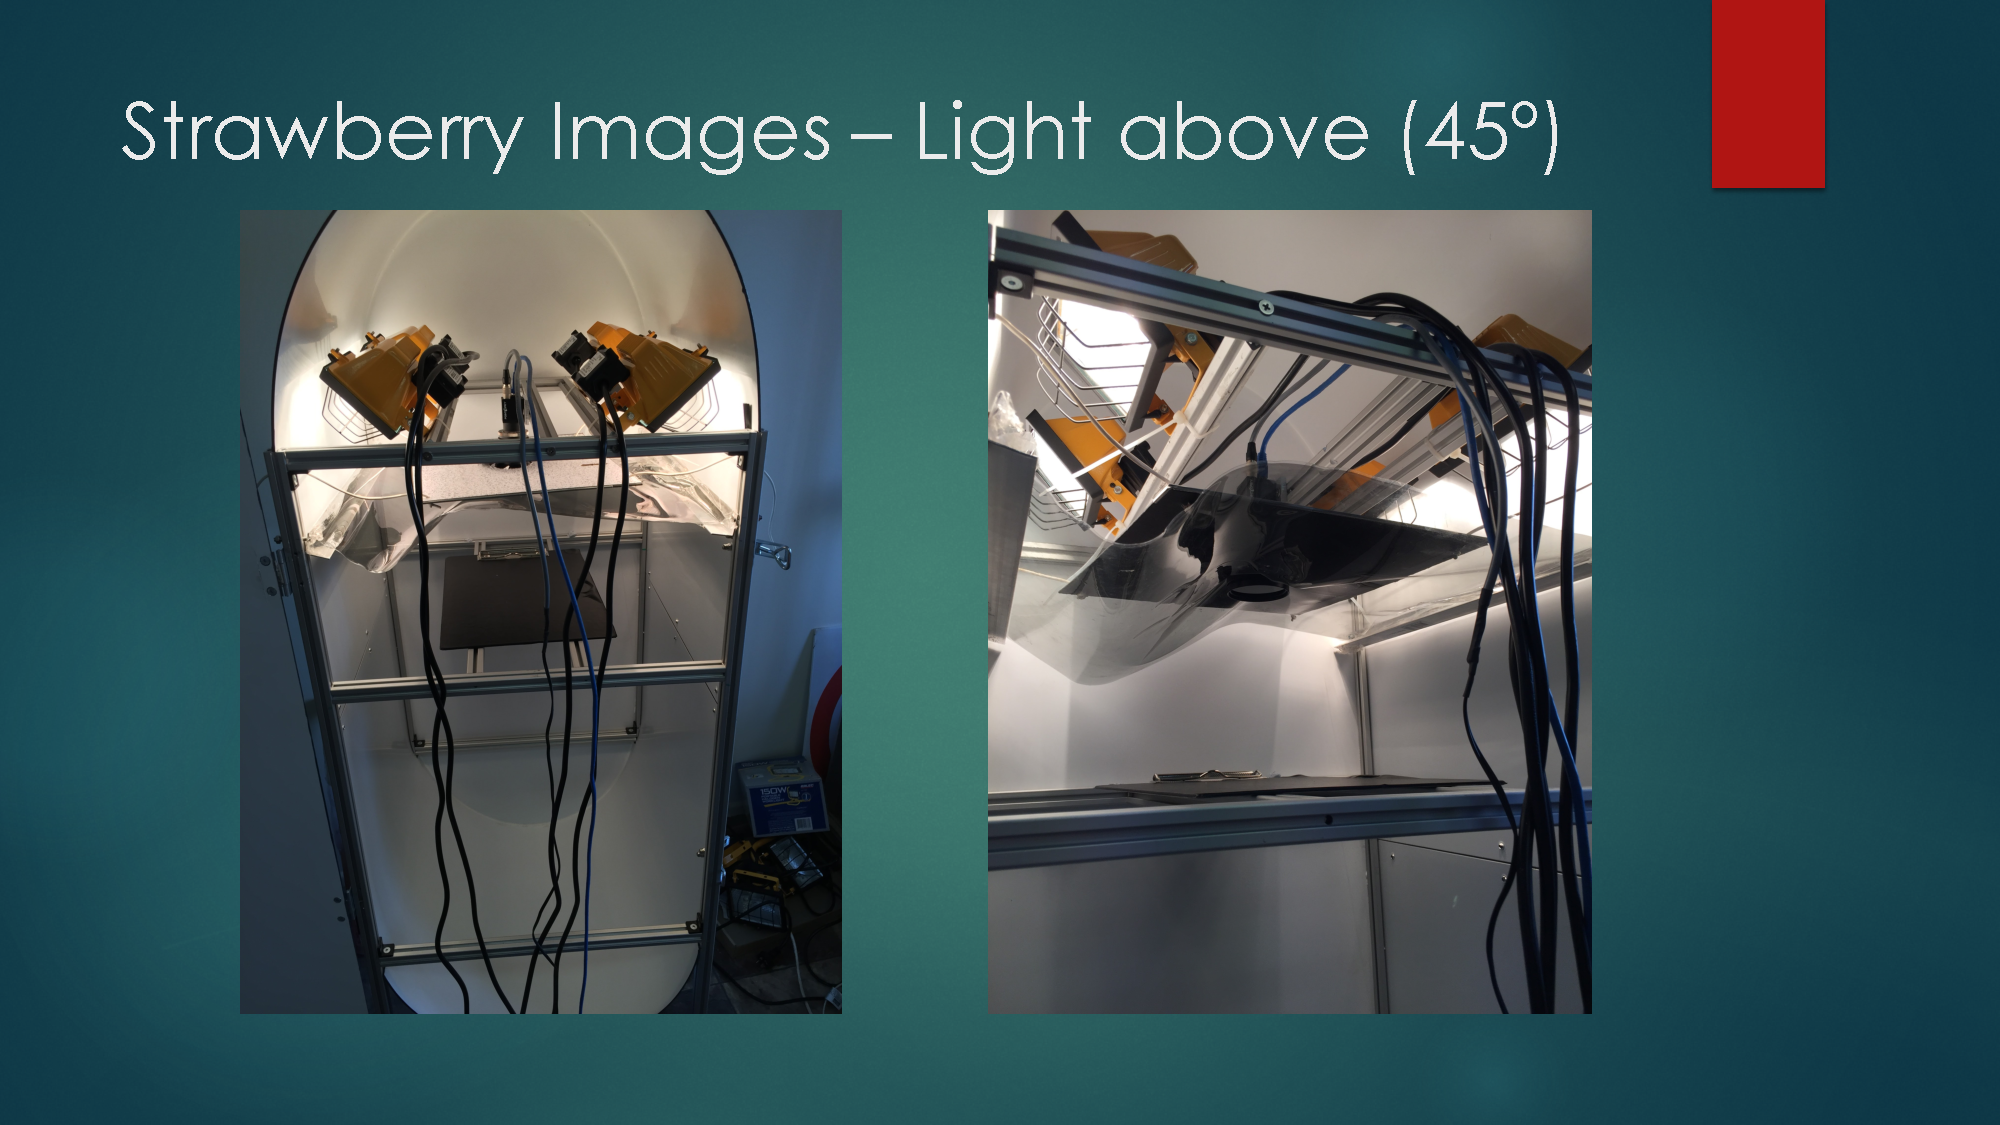
\includegraphics[width=\linewidth]{images/lighting_angle/45/45_degrees_setup.pdf} & \includegraphics[width=\linewidth]{images/lighting_angle/45/45_deg_polar.jpg} & \includegraphics[width=\linewidth]{images/lighting_angle/45/45_deg_cross_polar.jpg} \\
		
		3 &
		\includegraphics[width=\linewidth]{images/lighting_angle/90/90_degrees_setup.pdf} & \includegraphics[width=\linewidth]{images/lighting_angle/90/90_deg_polar.jpg} & \includegraphics[width=\linewidth]{images/lighting_angle/90/90_deg_cross_polar.jpg} \\
		
	\end{tabular}
\end{table} 

Initially the lighting systems used were powered by $240VAC$ halogen lamps. The four $150W$ lamps wasted much of the output given the wide spectral band of halogen devices. Moreover, the inherent flickering problem due to the alternating current, causes illumination differences from image to image. This was also observed during an experiment where the camera's shutter had been synchronised (as close as possible) to the $50Hz$ sinusoid from mains power.

Experimental testing provide visual representation of using different incident angles for the lighting sources with and without the cross-polarisation. Table \ref{tab:lighting_orientation} illustrates the lighting configurations used for $0^{\circ}$, $45^{\circ}$, and $90^{\circ}$ incident angles with single polarisation and cross-polarisation images for comparison. This clearly shows that the more direct the source is to the object, the greater the chance of shadows and specularity, leading to the optimal lighting angle of $135^{\circ}$ (directed upwards away from the target). The experiments also confirmed that the polaroid sheets are more consistent when rigid, opposed to thin, flexible versions. For example, when using the thin sheets in the examples from Table \ref{tab:lighting_orientation}, some leakage occurred originating from bent or warped sections of the polaroid. When straightened, the problem could be eliminated, however this is still not appropriate for the application given the material may expand over time with temperature, therefore rigid polarising sheets will be required.



\begin{figure}[h!]
	\centering
	\includegraphics[width=0.8\textwidth,angle=270]{bench_led_rigid.jpg}
	\caption{Final configuration of the visible lighting and polarising material.}
	\label{fig:final_led}
\end{figure} 

Figure \ref{fig:final_led} shows the configuration of the top automotive LED bars and rigid polarisers in place with the bottom lighting to be mirrored at a later stage. A combination of automotive led bars and small 12V halogen lamps are used to perform testing for intensity purposes, and to confirm the reduction in power is negligible due to the efficiency of LEDs. 



\begin{table}[h]
	\centering
	\caption{Comparison of power characteristics and intensity values when tested against lux meter readings as well as pixel thresholds in an image. There exists differences in beam pattern, mounting configurations, and spectral output, however the results are indicative for a target object and static camera.}
	\label{tab:AC_vs_DC}
	\begin{tabular}{lccc}
		\toprule
		Element & Halogen Lamps & LED + Halogen Lamps & Units \\
		\midrule
		Power Consumption per hour 	& 600 		& 344 		& $W$ \\
		Voltage						& 240  		& 12  		& $V$ \\
		Average Current				& 2.5		& 28.6		& $A$  \\
		Intensity Value (lux meter)	& 15		& 17		& $klx$  \\
		Pixel Value	(image region)	& 245		& 274		& $kpx$  \\
		\bottomrule
	\end{tabular}
\end{table} 


The LED lighting with supplementary halogen performed slightly better in terms of intensity alone, according to Table \ref{tab:AC_vs_DC} showing the overall increase in intensity and pixel value, even though there was a dramatic reduction in power consumption, due to the LED replacement. The intensity value measurement was obtained via a lux meter placed in the imaging platform of the prototype enclosure with closed doors, whereas the pixel value was calculated by region density of threshold by maintaining the same object and camera settings, averaging over 10 images. These methods will not be exact due to the physical changes and directionality characteristics, as well as spectral response differences between fully halogen and partly LED illumination, however results show the slightly increased performance of the new system in terms of subject illumination. 

Figure \ref{fig:final_image} is an example of the final image quality from the LED lighting only. The intensity is high enough to be able to set the shutter speed to an acceptable level without the addition of the smaller halogen lamps, which will increase the overall intensity even more.


\begin{figure}[h]
	\centering
	\includegraphics[width=0.8\textwidth]{final_image.jpg}
	\caption{Final image quality using $135^{\circ}$ lighting and cross-polarisation.}
	\label{fig:final_image}
\end{figure} 





\subsection{Camera Selection}

Flir\textregistered is a leading industrial, machine vision, surveillance, defence, and thermal camera company with a broad range of cameras to choose from depending on application. The Flir\textregistered cameras used for the SQA inspection are Blackfly\textregistered USB3 $2.3 MP$, 1920 x 1200, $41FPS$, with a Sony\textregistered IMX249 sensor capable of shutter speeds in the range $19\mu s-3.9s$ making it suitable for fast-paced applications. Quantum Efficiency (QE) of the monochrome model is approximately $10\%$ at $1000nm$ which is not ideal, but offers more spectral range and less noise at NIR wavelengths than other sensors. The cameras are powered via USB, which helps to reduce complexity, and include opto-isolated I/O for triggering. The comprehensive list of adjustable parameters make these cameras highly controllable or highly automatic, depending on user requirements, and can be programmed to function via software using the API packages. 

As the cameras have specific operating temperatures in the range ($0^{\circ}C-45^{\circ}C$), they will be susceptible to overheating and must be monitored (via the onboard temperature sensor, accessed using the API), particularly given that farm temperatures can reach $45^{\circ}C$ during the day. Therefore fans and peltier devices are added to the cameras in order to allow cooling if required. Intake fans apply positive pressure to the entire unit in an attempt to keep dust and dirt out of the acquisition area as lens/diffuser/polariser cleaning may become a common occurrence.


\subsection{Image processing}


The colour algorithm implemented uses the above visible image to determine ripeness based on colour features extracted via manual methods such as thresholding, segmentation, and morphology. This approach relies upon lighting intensity, and requires fine-tuning in the event of illumination changes. 

Using the HALCON\texttrademark IDE, the algorithms can be visualised before deploying them into production by utilising the debugging environment. When the method is finalised, it is converted to $C\#$ and inserted into the application as an \textit{external procedure}. Using HSV and CIE-Lab colour spaces, the analyses determine the amount of good and bad pixels with the help of pre-processing and post-processing techniques. The detection of defect region is largely based on the area of connected adjacent pixels which are found to be outside the acceptable bands of each optimal colour channel.   


\begin{figure}[h!]
	\centering
	\includegraphics[width=0.9\textwidth]{seg_4.png}
	\caption{The image processing algorithm including experimental calibration of size measurements.}
	\label{fig:seg_4}
\end{figure}  



The results indicate that the accuracy for under ripe algorithm will score $>80\%$, and over ripe at $>70\%$. As a quantitative test set of images has not yet been developed, the accuracy is based on a sample size of around 25-30 images per class. Further work is undertaken in order to increase the formal test set to approximately 500.   

Figure \ref{fig:seg_4} displays the results of blob detection/segmentation, morphology, colour analysis, and size measurements of the blobs. The calibration to real-world size uses camera pose information and was under development when the screenshot was taken.



\section{Conclusion} 


This chapter has detailed the quantified rate of acquisition and processing, indicating the shutter speeds and illumination intensity required for optimal image quality. The enclosure design and prototype construction has enabled research and experimentation into polarization, camera settings, motion blur, lighting intensity and configuration, streamlining efficient transfer to the production line when required. Design and development of the software and hardware frameworks have been performed with experimental results indicating the validity of using machine vision for quality inspection of full punnets of strawberries on a production line. 

Cross-polarisation and diffuse lighting arrangement have shown that, when sufficient illumination intensity is provided, eliminating specular reflections completely can be achieved, without diminishing image quality. In order to achieve this, constraining factors must be overcome such as high-speed acquisition, reflection generation including specular, stable lighting (flicker free), over-heating, and conveyor jogging. 

Individual and total power consumption is detailed in Table \ref{tab:DC_power_table}, identifying high-power DC supply requirements calculated. The investigation found that a high-powered computer PSU is sufficient to perform all the DC electronic tasks including lighting, and provides the additional benefits of electrical protections and highly configurable outputs.

Image processing algorithms have been integrated with the main application in order to create the image pipeline from cameras to assessment and finally display of results. Creating preliminary scripts utilising functions such as thresholding, morphology, and colour analysis have enabled initial image processing results based on bench images.


A control system has been implemented in order to perform the electronic switching of high-powered devices as well as pneumatic activation in order to eject the defected punnets, which depends on the ability of the main application to be able to perform asynchronous actions in a synchronous manner.



%%%%%%%%%%%%%%%%%%%%%%%%%%%%%%%%%%%%%%%%%%%%%%%%%%%%%%%%%%%%%%%%%%%%%%%%%%%%%%
%%%%%%%%%%%%%%%%%%%%%%%%%%%%%%%%%%%%%%%%%%%%%%%%%%%%%%%%%%%%%%%%%%%%%%%%%%%%%%

\newpage
\chapter{A Method To Create Stable Lighting And Remove Specular Reflections for Vision Systems}
\label{sec:paper_1}

\textbf{Gilbert Eaton, Andrew Busch, Rudi Bartels, and Yongsheng Gao}

\textit{Conference paper - Digital Image Computing: Techniques and Applications (DICTA) - accepted Aug 2017}


\section{Abstract}

\textbf{A lighting system and method has been developed which has shown in testing to allow quality images to be obtained that are free from two particular problems, specular reflections on the subject, and light intensity variation. These problems both diminish the ability to compare objects for attributes such as colour variation, edges, contours, and many other features. The system developed eliminates specular reflection by using the cross-polarisation configuration, and reduced flickering due to fluctuations in the power supply to negligible levels by constructing a high-power DC source capable of providing sufficient 12 Volt power. These two improvements create an environment suitable for taking high-quality, noise free images at high shutter speeds for the purpose of assessing the quality of strawberries moving on a real-time production line.}


\section{Background}


When using image processing to analyse images or extract features, one problem faced is the inconsistency of images \cite{atkinson}.  For example, when using AC lighting and fast shutter speeds, the image intensity will vary with the intensity of the alternating current in the power supply. Although undetectable to the human eye, this type of "flickering" can give rise to a vast difference in image intensity. Another example is that of specular reflection as shown in Figure \ref{fig:specular_art}. The bright reflection appears as white "interference" as the information contained in the pixels of this region are lost. The loss of information may include colour, edge contours, region boundaries or hidden defects. This paper is aimed at describing a method of eliminating these problems in order to increase consistency in acquired images.

Image stability is particularly required in industrial applications when performing defect inspections, or quality control processes. The environment surrounding the subject must be consistent, and free from saturation and specular reflections. Achieving this will then provide more valuable information and comparability of images due to the removal of noise and inconsistency.

The proposed system ensures that when objects imaged for computer vision applications, they do not contain specular reflections or saturation, and intensity is stable for comparison purposes. 

\begin{figure}[h]
	\centering
	\includegraphics[scale=0.9]{specular_art.jpg}
	\caption{Example of Specular Reflection on an art display. Note the specular reflection interference with the image causing the loss of information and colour.}
	\label{fig:specular_art}
\end{figure}


Specular reflections occur when the source of light can be seen on the surface of the object. This can be either a direct reflection from the light source onto the object and then into the viewer (eye or camera), or through multiple reflections where the light source is still visible. The direction of the specular reflection is related to Snell's Law, in that, the angle of incidence ($\theta_i$) is equal to the angle of reflection ($\theta_r$). These reflections are best seen on smooth surfaces such as glass, water, and metal whereas reflections from rough surfaces will result in a more diffuse spread.   

According to electromagnetic wave and transmission line theory, at the interface of a good conductor, the reflected field ($\bar{E_0^r}$ - Phasor form of the electric field in the z plane of incidence) at the interface of the medium is equal to the incident field ($\bar{E_0^i}$) subtract the transmitted field ($\bar{E_0^t}$) \cite{ulaby} where:

\begin{equation}
\bar{E_0^r} = \bigg(\frac{\eta_2 - \eta_1}{\eta_2 + \eta_1}\bigg)\bar{E_0^i}
\end{equation}

and for the transmitted field:

\begin{equation}
\bar{E_0^t} = \bigg(\frac{2\eta_2}{\eta_2 + \eta_1}\bigg)\bar{E_0^i}
\end{equation}


This shows that the intensity of the reflection is determined by the intensity of the source of the wave and the intrinsic impedance ($\eta$) of the material and is given by:

\begin{equation}
\eta = \frac{\omega \mu}{k} = \frac{\omega \mu}{\omega \sqrt{\mu \epsilon}}= \sqrt{\frac{\mu}{\epsilon}}
\label{eqn:eta}
\end{equation}

where the wave number $k = \omega \sqrt{\mu \epsilon'}$ and $\mu$ is the magnetic permeability of the material. This relates to its susceptibility to magnetic fields, and for diamagnetic and paramagnetic materials (which includes most metals and dielectrics), is considered to be the same as that of free space and $\mu = \mu_0 = 1$ \cite{ulaby}. 

The electric permittivity, however, is very small for most metals as $\epsilon = \epsilon_r \epsilon_0 = 1 \cdot 8.85\cdot10^{-12}$. Substituting this into equation \ref{eqn:eta}, maintains a large value for intrinsic impedance $\eta_2$. thus, the majority of the wave is reflected at this angle. This is comparable to a short circuit on a transmission line resulting in a reflection coefficient of -1 indicating a full reflection even though inverted. This shows that the intensity at the specular angle is not diminished very much by the surface of a smooth conducting surface.

However, one change that can occurs at the interface, is the polarization of the wave. All light sources are randomly generated in all orientations, and can therefore be said to be multi-linear, circularly, or elliptically polarised (commonly named un-polarised or non-polarised) waveform \cite{artusi,nelson}.


\section{Specular Reflections} 

\begin{figure}[h]
	\centering
	\includegraphics[scale=0.9]{unpolar_polar.png}
	\caption{The interface showing specular reflection of an electromagnetic wave in either the TE or TM orientation.}
	\label{fig:unpolar_polar}
\end{figure}

Figure \ref{fig:unpolar_polar} shows that when an un-polarized incident light ray reflects from a surface, the polarisation is converted to linear form, in the direction of the surface of the object \cite{nelson}.

As the total energy is maintained and the polarisation is converted to linear, the reflection is perceptively intensified in that direction. Multiple reflections can also contribute to this appearance of specular reflection hot spots on objects depending on the surfaces around them and the lighting orientation.

This is a problem for industrial areas where, for instance, on a production line sufficient lighting is required to illuminate the product for image processing purposes. Reflections can occur from the surrounding surfaces or objects, and can be subject to change if the environment surrounding the production line and cameras are rearranged, added or removed.


\section{Lighting Intensity Stability}

As discussed in Section \ref{sec:challenges}, alternating Current (AC) power sources have a sinusoidal pattern and have a frequency associated with them. This fluctuation is inherent in everyday power usage, such as the current in mains power supply (in most cases 110/220/240V @ 50/60Hz), and is very useful for long distance power transmission. Although this fluctuation can not be seen by the human eye, the fast shutter speeds of the vision cameras can. The difference in the images can theoretically be $100\%$, as the current passes through the zero point in the sinusoid.

The benefit to using AC lighting is that high power/high intensity lighting is easier to achieve. For example, $1000W$, $240V$/$50Hz$ AC lamps are readily available, however, a $1000W$, $12VDC$ lamp is substantially less common. This means that to achieve the same level of lighting as an AC system, a $12V$ DC system must be able to power many small LED, tungsten, or halogen lamps resulting in high current requirements.  


\section{Methods}

\subsection{Specular reflections}

Polarising material has been shown to reduce the effects of these reflections. If surface reflections of the light source are seen by the cameras, and not the direct light source, the polarising material can remove the specular reflections in one direction. This type of method has been used in experiments to try to improve the quality of images \cite{atkinson, wolff}.

Exploiting the use of a cross-polarising lens on the camera reduces the specularities even further. By controlling the polarity of the light hitting the objects' surface, and then again before the light enters the camera lens, the reflections in the image are minimised.

If the polarisation orientation is parallel throughout the the inner walls of the tunnel, then all light within the tunnel will have the same orientation of polarization. By adding a polarising filter to the camera lens at an angle orthogonal to the polarised walls, then the specular reflections are dramatically reduced \cite{anderson, kuranov}.


\subsection{Power Supply}


Preliminary testing gave a good indication of the lighting power requirements by testing many different lighting angles, intensities and polarization configurations. The tests showed that, in order to get adequate intensity through a cross-polariser, the power requirements in Table \ref{tab:DC_power_table} (Chapter \ref{sec:electronic_power}) are determined to be appropriate.

After initial bench testing, the calculated lighting power was around $688W$, with power draw from peripheral devices totalling approximately $750W$ in normal operating conditions. A $750W$ power supply would meet the operational requirements but leaves no room for variation in current such as inrush, and the potential to increase the amount of light sources in the future. Another requirement of the power supply is that it support $5V$ for peltier, fans, and micro-controller (Phidget), otherwise an additional power supply, or a high-powered, voltage divider circuit will be required.

It is for these reasons that a PC Power Supply Unit (PSU) was determined to best fulfil the requirement. A PSU generally supplies $12V, 5V$, and $3.3V$ as well as some models providing a $-12V$ low current line in order to generate $24V$ potential. These PSUs are designed for longevity, robustness and high power PC applications and hardware used to render video, or facilitate graphics-intensive, high resolution games. The Cougar\textregistered $1200W$ PSU is high quality and cost effective means to generate $100A @ 12V$ with the added attractive fault protection features. The relevant specifications are shown in Table \ref{tab:psu_spec}.


The PSU also has the following protections as part of the manufacturing specifications:

\begin{itemize}
	\item Over Voltage Protection - If the voltages increase above a certain tolerance value on the single lines, the PSU automatically switches off.
	\item Under Voltage Protection - If the voltages fall below a certain tolerance value on the single lines, the PSU automatically switches off.
	\item Over Power Protection - If the system is oversized and requires more power from the PSU than it can deliver, this protection function is activated.
	\item Over Current Protection - If the load on a single line is higher than indicated, the PSU automatically switches off.
	\item Short Circuit Protection - In the case of a short-circuit this feature prevents damage to the core components of the PSU and its system components.
\end{itemize}

\quad
\begin{table}[h]
	\centering
	\caption{Cougar $1200W$ Power Supply Unit (PSU) specifications}
	\label{tab:psu_spec}
	\begin{tabular}{l*{4}{c}}	
		\toprule 
		Specification & Min & Typ & Max & Units\\ 
		\midrule
		DC Output & - & - & 1200 & $W$ \\[6pt]
		Operating Temp. & 0 & 25 & 45 & $^{\circ}C$ \\[6pt]
		Efficiency & 80 & 87 & 90 & $\%$ \\[6pt]
		Transient 12V turn on & 7 & 9 & 10 & $ms$ \\[6pt]	
		Ripple 12V (100\% load) & 70 & 73 & 75 & $mV$ \\[6pt]
		Ripple 5V (100\% load) & 39 & 42 & 45 & $mV$ \\[6pt]
		Ripple 3.3V (100\% load) & 40 & 42 & 44 & $mV$ \\[6pt]
		
		\bottomrule
	\end{tabular}
\end{table}

\section{Results}

The $1200W$ DC power supply is designed and constructed so that the full power of the $12V$ rails are supplied by distributing each of the two channels between the top and bottom lighting circuits. The power supply also supplies power to peripheral devices such as pneumatics, LED indicators, warning lights, logic control board, sensors, peltier, and fans.

The resulting images taken using the designed enclosure have dramatically improved the image stabilisation when compared to the AC lighting system. The DC-powered lighting system resulted in very small intensity fluctuations, and was measured to be $<0.1\%$ as seen in Figure \ref{fig:image_diff_dc} and \ref{fig:image_diff_dc_2}. The average pixel area for each image was obtained by first taking a threshold of subjects in the each of the frames:
\begin{equation}
R = \sum_{i=1}^{P}t_1 \leq x \leq t_2
\end{equation}

with $P$ denoting the number of pixels in each image and $t_1$, $t_2$ the threshold limits. The average region area ($Area_{avg}$) was calculated and is given by the mean definition:
\begin{equation}
Area_{avg} = \bar{R} = \frac{1}{N}\sum_{i=1}^{N}R_i
\end{equation}

where $N$ is the number of images to average, and $R_i$ represents the number of region pixels in each image.

Data was gathered twice, once for a period of two seconds with a fast frame rate, and the other over a three hour period in order to assess the case of high speed cameras, and in the case of constant operation for extended periods of time.



\begin{figure}[h]
	\centering
	\begin{subfigure}{.45\textwidth}
		\centering
		\includegraphics[width=.95\linewidth]{image_diff_dc.png}
		\caption{}
		\label{fig:image_diff_dc}
	\end{subfigure}%
	\begin{subfigure}{.45\textwidth}
		\centering
		\includegraphics[width=.95\linewidth]{image_diff_dc_2.png}
		\caption{}
		\label{fig:image_diff_dc_2}
	\end{subfigure}%
	\caption{Intensity measurements taken using DC lighting system showing the small variations over: a) A two second period and b) A 3 hour period. All results have a difference of less than 0.1\%.}
	\label{fig:test4}
\end{figure}

\begin{figure}[h]
	\centering
	\includegraphics[width=.7\linewidth]{polarizer_rot.png}
	\caption{Experimental results gathering the specular and region pixels, whilst rotating the cross-polariser on the camera lens.}
	\label{fig:graph_polar}
\end{figure}

\begin{figure}[ht]
	\centering
	\begin{subfigure}{.4\textwidth}
		\centering
		\includegraphics[width=.9\linewidth]{berries_spec.png}
		\caption{}
		\label{fig:berries_spec}
	\end{subfigure}%
	\begin{subfigure}{.4\textwidth}
		\centering
		\includegraphics[width=.9\linewidth]{berries_no_spec.png}
		\caption{}
		\label{fig:berries_no_spec}
	\end{subfigure}%
	\caption{Image of strawberries (a) with specular reflections and (b) without specularities after the cross polariser was added.}
	\label{}
\end{figure}

In order to solve the specular reflection problem, the use of a cross-polarization lighting design was implemented. As discussed in Section \ref{sec:I}, polarizing material is installed vertically (polarization direction can be either orientation, although further testing may indicate a preference) to form a tunnel through the enclosure. The second polariser is an adjustable filter fitted to the lens of the visible camera. The graph shown in Figure \ref{fig:graph_polar} shows that when the specular pixels are removed, the region pixels are increased giving a better assessment of the area of interest.



Figure \ref{fig:berries_spec} shows an image with only one polariser in place allowing some specular reflections to be seen (the amount of specularities would be even greater if the acquisition had no polarizing elements), then by rotating the camera lens polariser, images were taken at 16 positions from $0^{\circ}$ to $180^{\circ}$.  


When the polarisers are orthogonal ($90^{\circ}$), the result is a more flattened image that removes the specular reflections almost entirely.  Figure \ref{fig:berries_no_spec} depicts this change and it can be seen that the surface of the strawberries are much clearer and will allow better image processing due to the increase of pixels which can be analysed, and a decrease in noise. 



\section{Conclusion}

Image acquisition plays an important part in any machine vision application to ensure that the images acquired are free of distortion and provide the most information. Lighting is therefore an important factor in image acquisition systems, allowing objects surfaces to be illuminated with as little interference as possible.

A system has been developed to inspect strawberries and assess them for quality attributes. The first step in the development is to design and construct the acquisition system and integrate it with the production line. After the enclosure had been installed, the LED/halogen lighting, polarisers, and cameras were mounted. The DC power supply delivers the required amount of power at a constant current which ensures that the intensity fluctuations between images are insignificant. Experimental results show that the fluctuations are less than $0.1\%$ of total intensity, even when operating for many hours. Experiments were also performed that showed that the cross-polarization technique has the ability to entirely remove of the specular reflections in most cases, whilst providing more pixels that can be analysed in each frame.  

The system developed is extremely successful in achieving the desired consistent image acquisition. The system can image 2 punnets of strawberries per second on the production line and the image quality is illuminated, free from interference, and consistent between images, even with a shutter speed as fast as $1ms$. Future work includes the strategy to strobe the lighting in order to reduce power usage and heat, as well as the introduction of image processing algorithms to perform the assessment.



%%%%%%%%%%%%%%%%%%%%%%%%%%%%%%%%%%%%%%%%%%%%%%%%%%%%%%%%%%%%%%%%%%%%%%%%%%%%%%
%%%%%%%%%%%%%%%%%%%%%%%%%%%%%%%%%%%%%%%%%%%%%%%%%%%%%%%%%%%%%%%%%%%%%%%%%%%%%%

\newpage

\chapter{Production Integration}
\label{sec:II}

\section{Introduction}

In order for a successful implementation and installation of the new plant equipment on the production line, a seamless transition is preferred in order to maintain control and flow of produce. As the SQA integration works could present disruptions or interruptions to production - due to traffic around the machine, power tool use, and construction materials being transferred into and out of the packing room - the process must be managed well. This will require strategies such as utilising early mornings (when picking is occurring) and non-picking days to perform noisy, potentially contaminative construction works, whilst reserving the less intrusive activities such as testing component functionality, electrical wiring, and fine-tuning, to be performed during production.


Work in this chapter builds on the implementation of research and experiments conducted in Chapter \ref{sec:I} with the main component's configurations determined. Firstly, the power supply unit must operate the required high power systems simultaneously in order to confirm the operational load is satisfied by the power provided. The cross-polarisation is a key attribute of the system and is required to be fine-tuned once the cameras and polaroid sheets are in place. This will be performed by using a live view of the cameras focussed on a reflective object whilst turning the lens polariser, until all specularities are eliminated. Likewise, the motion blur, overall intensity, and camera triggering will require installation, assessment, configuration, and confirmation of expected operation, where unobstructed daily production data capture are the key outcome success factors.


\section{Integration Topology}
  

The strawberry packing facility consists of two large chillers, four packing benches and a large area for wrapping and labelling pallets. As the berries are picked in the field, they are placed in large trays of approximately $5kg$. The trays are loaded onto racks to be transported to the packing room chiller and eventually packed into smaller containers. The packing room floor plan is shown in Figure \ref{fig:pack_layout_1}, with the flow of berries (indicated by arrows) from chiller to packing benches, followed by the wrapping station, and finally the storage chiller. The trays are delivered to the four packing benches and are accumulated in the centre of the eight packing stations on each bench. The QA personnel positioned at the end of each bench will load the trays of packed punnets onto pallets, and signal operators to collect them when full. The pallets are then recorded, wrapped and labelled in a large designated space before being loaded into the finished product chiller, ready for transportation.


\begin{figure}[h]
	\centering
	\includegraphics[width=.95\linewidth]{Pack_layout_1.png}
	\caption{Packing room configuration before introduction of the Heat-seal and SQA system.}
	\label{fig:pack_layout_1}
\end{figure}%


The SQA vision system and heat-seal machine are required to process the punnets after packing has occurred and before palletisation, indicating their placement on the production floor is essential. An alternative to this process includes off-site processing of both quality vision system assessment and sealing of containers, but would require extra transportation and potential for contamination or wasted packaging. Fortunately, rearrangement of the wrapping area is possible due to the large space usually reserved for staging of empty boxes and wrapping and labelling pallets of finished product. Figure \ref{fig:pack_layout_2} shows the floor plan with the addition
of the SQA system and Heat-seal machine, reducing the available storage and wrapping space, whilst maintaining production requirements.


\begin{figure}[h]
	\centering
	\includegraphics[width=.95\linewidth]{Pack_layout_2.png}
	\caption{Planned packing room configuration after Heat-seal and SQA system have been positioned.}
	\label{fig:pack_layout_2}
\end{figure}%


This arrangement does not impact the production speed (as per system requirements) due to the simple redirection of produce. Previously, the palletised containers were taken from the ends of each packing bench to the wrapping area, labelled, and put into storage awaiting transport. After the configuration changes, the pallets are taken to the SQA conveyors and processed by both plants, before accumulating on a large circular table and being palletised and processed as usual. These two systems add value to the product by automatically performing the following:

\begin{itemize}
	\item SQA vision system removes defected punnets for repacking as a final quality assurance step, reducing customer complaints, stock returns, and brand diminishment. 
	\item Heat-seal machine seals plastic film onto the punnet in order to eliminate tampering.
	\item Metal detector placed after Heat-seal removes punnets in the event of contamination by either plant.
	\item Final weight checking removes punnets if the scale detects out-of-specification items.
\end{itemize}  


Although the addition of these systems require the increase of labour by two persons (and purchase of equipment), the benefits moving to an automated, consistent, quality assurance and sealing machine are not only seen by the producer, but also the customers who retail and consume the goods.


\section{Production Floor Migration}

Migration from prototype to production-ready equipment is a difficult task given the constant high volume throughput in many facilities. Vision quality systems are typically adopted when the production volume becomes too great for human workers to maintain detailed inspections given some application process rates are faster than human sensory perception can comprehend \cite{sofu, duan}. However, the addition of such systems causes intrusions on the production line such as reduction of available floor space, slowing or stopping line speed, safety hazards, and rework. Additionally, if the system contains faults, the impact is much greater potentially causing injury, property damage, loss of revenue, or sub-standard product.

Mean Time Between Failure (MTBF) is a term used by maintenance professionals defined as the predicted average time for which a system (or component) performs its function in production before failure, or mathematically:
\begin{equation}
	MTBF = \frac{\sum (\text{downtime} - \text{uptime})}{\text{number of failures}}
\end{equation}

This metric is evidence of the emphasis companies put on production flow and continuity. If systems under-perform they are at risk of being replaced or eliminated in order to allow production to produce at optimal rates. Given these risks to the system adoption, the process of transition must be performed in an efficient manner, whilst creating a non-restricting addition to production that can perform accurately. Implementation of the production-ready enclosure required the prototype to be fit with conveyors, lighting, power systems, diffusers and polarisers, as well as the computer systems, sensors and cameras. Once the designs were complete, bench testing of the equipment such as camera image transmission to the running application, microcontroller functions including camera triggering and lighting switching, power system and peripherals was performed, reducing delays when installation occurs on the busy production line.


Initially, the conveyors were added to the frame in order to create the path of flow for the punnets, as shown in Figure \ref{fig:system_construct_3}. The frame of the prototype was adjusted slightly in order to equal the height of the conveyor where it meets the v-belts, as well as centred on the conveyor relative to the enclosure. All heights are consistent with other machinery and conveyors in the packing shed to allow many possible configurations in the process flow. 



\begin{figure}[h]
	\centering
	\includegraphics[width=.5\linewidth]{system_construct_2_2.jpg}
	\caption{The frame of the enclosure shortly after the conveyors had been attached. The v-belts have also been installed and are visible, mounted higher than the conveyor belt in order to suspend punnets by their lips.}
	\label{fig:system_construct_3}
\end{figure}%


A wide range of conveyors, motors, guide rails, and parts were made available (due to the farm equipment spare parts), and assisted the construction of the punnet conveyors, and their attachment to the frame of the enclosure. However, the v-belts are a customised feature using brackets to support adjustable grooved rollers designed for the shape of the belt, and a guide rail on each side to avoid sagging due to punnet weight. The point of transfer, where the v-belts meet the punnet conveyors, must be considered in order to implement a smooth transition at both the entry and exit of the enclosure. The requirement is for the punnet to enter the heat-seal machine long-edge leading (due to cost-saving design), but this is problematic for the v-belts in the case where a  punnet enters incorrectly oriented, and too narrow to be transferred onto the v-belts. Therefore, the design was to employ a $90^{\circ}$ transfer belt between the vision system and heat-seal machine, allowing the punnets to be short-edge leading as they enter the enclosure, eliminating the risk of containers falling between the v-belts (seen in Figure \ref{fig:pack_layout_2}). 


Two $100W/240VAC$ conveyor motors are used with slightly different gear ratios. The in-feed conveyor and v-belts are driven by the same motor, whilst the out-feed conveyor is driven slightly faster (using a smaller sprockets) in order to separate the punnets in case of ejection.


The ejector mechanism must be positioned some time after the vision inspection, given that the v-belts prevent any dislodgement, and the added complications associated with adding ejector mechanisms in the acquisition section. Therefore the ejection must occur on the out-feed conveyor, generated by a pneumatic burst of air from the side, pushing it in a direction perpendicular to the motion of flow, onto a roller-ramp which then guides the punnet into an accumulation area. Both the ejector and acquisition system activate when a punnet passes the photo-electric sensor. In the case of ejection, the microcontroller must be synchronised with the running application to determine which punnets to eject and will only activate the pneumatics when defects are detected. The acquisition system generates a sequence of imaging - through the hardwired triggering mechanism attached to the I/O port of each camera - in order to capture the different views and spectra of each punnet, followed by instigating the image processing and display routines within the application. 


\subsection{Electronics and Power}

The DC electronic power must support the system on the production floor independently, allowing for the encapsulation of system components in the busy work environment. The lighting, sensors, conveyors, computer, and control systems must all be contained within the small footprint provided, with no available form of power other than the $240VAC$ mains supply. Design of the power supply and electronic box (Chapter \ref{sec:electronic_power}) is such that it is small enough to fit beneath the enclosure without protruding in any direction. 


The main electronic devices can be seen in Figure \ref{fig:system_construct_1} where final testing took place before they were installed. Once confirmed, the PSU was mounted and reconnected to the distribution devices and ground bars. The LED's and halogen lamps wiring has a $3.5mm$ diameter core designed for high current to avoid any thermal concerns in the already heated environment. Each LED bar is installed with it's own power line directly to the distributor, however it is more efficient and simplified to wire the halogen lamps in pairs (equalling the current for one LED bar). This standardises the current flow, on any one of the eight lines in total, to approximately $6A$, meaning that $7.5A$ automotive fuses were suitable protection, given they can withstand the inrush on start-up. 


\begin{figure}[h!]
	\centering
	\begin{subfigure}{.59\textwidth}
		\centering
		\includegraphics[width=.9\linewidth]{system_construct_1.JPG}
		\caption{}
		\label{fig:system_construct_1}
	\end{subfigure}%
	\begin{subfigure}{.39\textwidth}
		\centering
		\includegraphics[width=0.8\linewidth]{enclosure_3.jpg}
		\caption{}
		\label{fig:system_construct_2}
	\end{subfigure}%
	\caption{System integration stages (a) testing all lighting powered at once by the PSU prior to installation , (b) all LED's in place as well as polarising material/diffusers, and a single camera installed before the addition of halogen lamps. Extra cladding added to both remove external lighting noise, and cover potential pinch-points.}
	\label{}
\end{figure}



Smaller LED bars ($30W$ opposed to $72W$) were required to be installed in the mid section of each side of the enclosure (shown in Figure \ref{fig:system_construct_2}) in order to generate more side lighting, and bring the total illumination power to a comparable level calculated by using data from the halogen experiments. Given that the main LED's were upward-facing, the illumination diminished significantly from the sides of the conveyor, which lead to images with shadowy occlusions particularly around the edges of the punnet. These four devices were also paired together, occupying two outputs on the distribution device. 


Figure \ref{fig:system_construct_2} shows the main, and auxiliary, LED's installed along with an RGB camera in order to perform lighting tests. The diffusers and polarising sheets are sandwiched together and form a rectangular tunnel around the acquisition chamber, with the intense lighting outside being diffused as it passes through creating a polarised tunnel. The external cladding (powder-coated steel sheets) covers each end of the lighting enclosure (above and below) and protrudes out from the rollers around the conveyors for safety purposes. 


\subsection{Lighting Finalisation}


With the LED's in place and acquisition tests performed, the halogen lamps and brackets are added to the exit end of the enclosure in order to provide the wavelengths required for the infrared cameras. The $35W/12VDC$ halogen lamps are designed for downlights for kitchens and showrooms (due to their large spectrum of illumination, giving a full colour appearance) using a lens with a $35^{\circ}$ aperture, in order to deliver a narrow floodlight beam. They have two pins to connect to the wiring or ballast, which push in to a connector comprising of spring-loaded friction terminals to hold the bulbs in place. The brackets help the lamps to face downward at an angle of $45^{\circ}$ relative to the cameras using the theory that diffuse lighting, rather than direct, would be better to avoid specularities (Figure \ref{fig:halogen}). IR images will have less specular reflections due to the surface penetration properties found at IR wavelengths, however they may still occur. Both the polaroid sheets and the dark-field lighting strategy help to minimise the event of unwanted reflections.

\begin{figure}[ht]
	\centering
	\begin{subfigure}{.5\textwidth}
		\centering
		\includegraphics[width=.8\linewidth, angle=270]{halogen.jpg}
		\caption{}
		\label{fig:halogen}
	\end{subfigure}%
	\begin{subfigure}{.5\textwidth}
		\centering
		\includegraphics[width=.8\linewidth, angle=270]{system_construct_3.JPG}
		\caption{}
		\label{fig:lights_power}
	\end{subfigure}%

	\caption{(a) The halogen lamps in place at an angle of $45^{\circ}$, (b) Completed lighting arrangement with PSU, distributors, and fuses mounted in electrical box.}
	\label{}
\end{figure}


The final steps for the installation of the lighting systems required wiring and connection to the PSU distribution device. Figure \ref{fig:lights_power} shows the operation of each required LED bar and halogen lamp powered by the PSU, after running the appropriate power wiring to length. Cable management and labelling practices have been used in order to give the system a clean and well-designed appearance, added to the value it gives to the process of methodical rewiring or fault-finding.



\subsection{Electronic Control System}


The microcontroller must perform physical electronic tasks which are required for the application including pneumatics, lights, and physical buttons. Each item may differ in power requirements, ranging from $3.3V-24V$ in both low and high current capacities. Therefore, a relay bank is used to switch the high-powered circuits such as lighting, whilst the Phidget\texttrademark's outputs can accommodate medium and low-powered devices. 


A programmatic looping worker thread services each I/O port periodically by performing three tasks; checking errors from microcontroller and other threads, processing interrupts generated by peripheral inputs, and processing output actions when required. The I/O worker thread is spawned from the main program which loops at $200ms$ per iteration. Each cycle, the worker uses the Phidget\texttrademark API call \textit{IsAttached()} method to check if the device is attached to the running application. If it is not, the input interrupt cannot be registered and the actions will not occur, therefore, an error message is displayed and the program must re-start. Although this is not a common failure, it is required in order to prevent I/O communication problems in future given the long hours and constant usage. This worker also monitors the health of the remaining threads which perform acquisition and image processing. 

The majority of inputs are generated by automatic processes (punnet sensors and heat-seal signal), however, the emergency stop button is wired to the conveyor power system, via a switched $240V$ device, in order to have the ability to stop them in an emergency, using a dry-contact activation so any circuit which closes/opens will activate it. The punnet sensors use a $685nm$ beam with reflector that, when broken, can either transition low-to-high or high-to-low depending on requirements. All three sensors are powered directly by the PSU with the output signal connected to the input port of the microcontroller. 


\renewcommand{\arraystretch}{0.8}% Tighter table height
\begin{table}[h]
	\centering
	\caption{Microcontroller INPUT port assignments and peripheral devices power ratings.}
	\label{tab:micro_pinout_in}
	\begin{tabular}{lcccc}
		
		\toprule
		\textbf{Element}  & \textbf{Port No.} & \textbf{Voltage ($V$)} & \textbf{Current ($A$)} & \textbf{Power ($W$)}\\[8pt]
		\midrule
		Emergency Stop Button 	& 0 & 12 & 0.001 & 0.012  \\[4pt]
		\midrule
		Heat Sealer 			& 2 & 24 & 0.5 & 12 \\[4pt]
		\midrule
		Eject Sensor 			& 4 & 12 & 0.1 & 1.2  \\[4pt]
		\midrule
		Punnet Sensor 1 		& 5 & 12 & 0.1 & 1.2 \\[4pt]
		\midrule
		Punnet Sensor 2 		& 6 & 12 & 0.1 & 1.2  \\[4pt]
		\midrule
		\textbf{Total} 			&   &    & \textbf{0.801} & \textbf{15.612} \\[4pt]
		\bottomrule
		
	\end{tabular}
\end{table}


The heat-seal machine has a jogging mechanism to control the punnets entering the sealing press. This means that the infeed conveyors stop periodically when the press is full, creating a convergence point for the punnets which could result in a backlog. Therefore, a signal line is sent to the microcontroller so that the conveyor of the vision system mimics that of the heat-seal. The listed requirements and voltages/currents for the Phidget\texttrademark inputs are detailed in Table \ref{tab:micro_pinout_in}.

High-powered devices are controlled by the Phidget\texttrademark in conjunction with a relay bank, in which the logic level input that drives the activation of the load requires $5V$ at $70mA$ current. The relays are rated at up to $250VAC/10A$ and $30VDC/10A$ restricting each relay to control either one LED bar ($6A$), or one pair of halogen lamps ($5.8A$). This would mean 10 relays would be required to perform this switching of components that was not necessarily needed to be automatically controlled. Therefore the LED bars and halogens were attached directly to the PSU so that they are powered continuously, and given that the PSU has an independent power switch, the illumination can be restricted to operational times only. The peltier and pneumatics remain as the next biggest loads and are therefore connected to the relays in order to prevent possible overload on the microcontroller, bringing the required number of relays to three. The outputs of the microcontroller and respective power loads are listed in Table \ref{tab:micro_pinout_out}.


\renewcommand{\arraystretch}{0.8}% Tighter table height
\begin{table}[h]
	\centering
	\caption{Microcontroller OUTPUT port assignments and peripheral devices power ratings.}
	\label{tab:micro_pinout_out}
	\begin{tabular}{lccccc}
		\toprule
		\textbf{Element}  & \textbf{Port No.}  & \textbf{Relay} & \textbf{Voltage ($V$)} & \textbf{Current ($A$)} & \textbf{Power ($W$)}\\[8pt]
		\midrule
		Conveyor Power Switch 	& 0 & No & 5 & 0.001 & 0.005 \\[4pt]
		\midrule
		Pneumatic Solenoid 		& 1 & Yes & 5 & 0.07 & 0.35 \\[4pt]
		\midrule
		Traffic Lights 			& 2 & No & 12 & 0.001 & 0.012 \\[4pt]
		\midrule
		Buzzer 					& 3 & No & 12 & 0.001 & 0.012 \\[4pt]
		\midrule
		Top Cooling 			& 4 & Yes & 5 & 0.07 & 0.35 \\[4pt]
		\midrule
		Bottom Cooling 			& 5 & Yes & 5 & 0.07 & 0.35 \\[4pt]
		\midrule
		\textbf{Total} 			&    &     &   & \textbf{0.213} & \textbf{1.079} \\[4pt]
		\bottomrule
		
	\end{tabular}
\end{table}


Power supply, fuses, relays, and microcontroller circuits are physically protected and fixed inside a plastic electronics case in order to simplify the wiring as well as keeping the relay board in close vicinity to the microcontroller pins which activate them. As the pneumatics are powered by $12V$, and the peltier by $5V$, a connection from the second distribution device (as well as the $5V$ terminal) to the normally-open terminals of the relays are made, before running together out of the box, to their respective components. The relays have three input pins ($5V$, $GND$, and Signal), and three output terminals (Normally Open (NO), Common (C), and Normally Closed (NC)) with a small LED to indicate activation of each relay, being extremely useful when testing and debugging the activation of peripheral devices. 

The $5V$ and $12V$ fuse boxes and connections are seen in Figure \ref{fig:PSU_5}, which are used to power the relays, whilst the signal is generated by the Phidget\texttrademark microcontroller. Eight $5V$ power lines from the PSU were bundled into two connections (as this is a more common voltage), and eight $3.3V$ bundled into one connection ($3.3V$ fuse box is not shown in the diagram as there are no devices connected to it, but allows future modifications and electronic additions if required). 


\begin{figure}[h]
	\centering
	\includegraphics[width=.9\linewidth]{PSU_schem.png}
	\caption{Schematic diagram of Power Supply Unit illustrating connections, fuses, distribution devices, $5V$ and $3.3V$ terminals as well as the microcontroller and relay box.}
	\label{fig:PSU_5}
\end{figure}

The PSU specifications table states that the maximum current for either $5V$ or $3.3V$ channel is $25A$ and they must share $160W$ load. Similarly, either of the $12V$ rails can supply up to $60A$ each but must share a total load of $1176W$, giving the power system the ability to dynamically distribute power as required, as well as the ability to reconfigure or add devices easily.


Wiring diagrams provided in Appendix \ref{app:wiring} detailing the complete wiring configurations across their different versions.



\subsection{Cross-polarization of RGB Cameras}


The polaroid sheets have a direction of polarisation, which usually runs parallel to one of the edges of the sheet, that is, either horizontally or vertically polarised. The polarity must be continuous on all sides, above and below the acquisition chamber in order to be effective when the cross-polariser is applied. The cross-polarising element used is a camera lens filter polariser which can be rotated $360^{\circ}$. This means that the cameras can be mounted in any orientation, and still achieve the desired result by rotating the filter (Figure \ref{fig:nd_filters}).


\begin{figure}[h]
	\centering
	\includegraphics[width=0.7\textwidth]{cross-polariser.png}
	\caption{Example of the polarising filter used on the camera lens which can be rotated to achieve cross-polarisation regardless of camera orientation.}
	\label{fig:nd_filters}
\end{figure}

As described in Chapter \ref{sec:I}, the polarising material transforms the incoming light from multi-polar to single polar form, which reduces the amount of specular reflections on any object thereafter. However, after applying another polariser orthogonal to the first, no specularities remain visible regardless of the multiple curvatures in the surface of the strawberries as seen in Figure \ref{fig:berries_no_spec}. 


The cameras are positioned in the centre of the respective lighting clusters in terms of spectral range in order to provide the best lighting response for each image. Therefore the RGB and IR are separated by a distance approximately $400mm$, complicating the asynchronous acquisition process.



\subsection{Motion Blur} 

The strawberry punnets used are $12cm\times 13.5cm$ which correlates to a pixel resolution of $1000x1200$ within the fixed field of view of the cameras. In order to calculate the motion of an object in an image, we take the product of the velocity and shutter speed:
\begin{equation}
M = V_p t_s
\label{eq:motion}
\end{equation}  

where the motion ($M$) units are relative to velocity ($V_p$) units (for example: pixels, $mm$, or $\%$), and the shutter speed ($t_s$) is relative to the movement in time. 

For the punnet length in centimetres $P_{cm}$, and the punnet length in pixels $P_p$, obtaining the value for pixels per centimetre in the direction of travel is:
\begin{equation}
P = \frac{P_p}{P_{cm}} = \frac{1000}{12} = 83.33 pixels/cm
\end{equation}

Calculating the pixel velocity per second in relation to line speed, the product of pixels per centimetre and line speed is:
\begin{equation}
V_p = L \times P = 28 \times 83.33 = 2333.33 pixels/sec
\end{equation} 

where $L$ is the production line speed of $28cm/sec$. Therefore, in order to find the shutter speed for one pixel of movement we rearrange \ref{eq:motion}:
\begin{equation}
t_s = \frac{M}{V_p} = \frac{1}{2333.33} = 0.000428572 \approx 0.5ms
\label{eq:shutter}
\end{equation}

where one pixel of movement over the distance of the punnet is equivalent to $\frac{1}{1000} = 0.001 = 0.1\%$. This shows that in order to generate zero motion blur, a shutter speed of $<428\mu s$ is required.



\begin{figure}[h]
	\centering
	\includegraphics[width=0.9\textwidth]{blur_1.jpg}
	\caption{Example of image captured with the shutter speed at $5ms$. This results in slightly blurred edges including seeds, berry lines and calyx, and reduces image quality.}
	\label{fig:blur_1}
\end{figure}

Using Equation \ref{eq:shutter}, the motion blur of one pixel is $~0.5ms$ which accounts for a $0.1\%$ difference. The image displayed in Figure \ref{fig:blur_1} has minor blurring resulting from a $5ms$ shutter speed, and is calculated to have $11.6$ pixels of movement or $1.16\%$ blur. 


This motion blur is in contrast to the image in Figure \ref{fig:sharp_1} where the shutter speed is reduced to $2ms$ and shows the seeds and edges clearly, albeit still blurred according to the calculation. Therefore any shutter speed less than $2ms$ will be sufficient to perform the analysis given that that means the motion blur is $4.66$ pixels which calculates to $\frac{4.66}{1000} = 0.00466 \approx 0.5\%$.

\begin{figure}[h]
	\centering
	\includegraphics[width=0.9\textwidth]{sharp_1.jpg}
	\caption{Example of image captured with the shutter speed at $2ms$. This reduces blur and the details are seen clearly.}
	\label{fig:sharp_1}
\end{figure}


\subsection{Image Synchronisation}
\label{sec:img_sync}

Each punnet consists of four image files (one for each camera), and must be compiled and saved together for quality traceability requirements (Chapter \ref{sec:requirements}). Therefore, each image is saved into a folder accompanied by a text file detailing metadata regarding statistics of the punnet such as date/time of images and classification information. The application saves the images and text file after population occurs via the two asynchronous threads generating RGB and IR images separately. 

However, some of the punnet's images failed to match initially, resulting in IR images which were not related to the RGB. When debugging the problem in the IDE it was found that if one set of images is received from the cameras and the others are not, the process would force the application to wait until the next punnet to populate the previous information. This is due to the triggered camera method, which waits for the image buffer indefinitely before proceeding, then returning to wait again some short time later. If the trigger does not occur, the thread logic continues to wait for the next trigger, leading to the conclusion that one of the punnet sensors was faulty or incorrectly calibrated. This was tested by monitoring the sensor's output via a wired connection from the sensor to the microcontroller. 

Experiments revealed that the both sensors had intermittent detection problems where they would not respond well in full-speed conditions. Trouble shooting performed included reflectance confirmation, calibration, independent power supply, and replacing sensor units, without success. As it was concluded that it was the environment creating errors (due to the metal surroundings and close proximity to objects) a redesign would be required to be refit them inside the enclosure. However, a machine vision solution exists to solve this problem, given that the punnets flow in the same direction seen by a fixed camera. Optical flow is a method of tracking moving objects by analysing the image differences in a stream. That is:
\begin{equation}
D_{image} = I_{n+1} - I_n
\end{equation}

where the difference image ($D_{image}$) is the result, and $I_n$ the image number in the stream, showing pixels with spacial variance (the moving objects) in an otherwise stationary scene. By analysing the difference regions, the punnet could be centred and acquired accurately, even though an extra time resource was taken up by the additional algorithm. This extra process added to the RGB thread does not impede the image processing algorithm which is the most time consuming element of the application. This is due to the threaded assignment of tasks such that the RGB acquisition thread can wait for a new punnet to be in position (optical flow processing), then capture the images required, whilst the image processing thread is assessing the previous punnet. The only constraint is that the image processing is complete before the punnet reaches the eject sensor.



 

\section{Final Configuration}


Testing the $90^{\circ}$ conveyor arrangement resulted in a change of conveyor configuration. If packed at production rates, each punnet collides with the next during the conveyor transition creating a randomly varying angle of orientation. It is imperative that punnets enter the heat-seal long edge leading (as per the requirements), as failure means stopping the production line in order to retrieve the incorrectly oriented container.

Therefore the v-belts and rail spacing required adjustment to the length of the punnet, rather than the width, creating the problem of miss-transfers and falling containers. This was addressed by adding a punnet-catching platform angled downwards from the entry transition point. Figures \ref{fig:inside_enclosure_1} and \ref{fig:inside_enclosure_2} show the punnet catcher and an in-line view of the enclosure.


\begin{figure}[ht]
	\centering
	\begin{subfigure}{.5\textwidth}
		\centering
		\includegraphics[width=\linewidth, angle=270]{inside_enclosure_1.jpg}
		\caption{}
		\label{fig:inside_enclosure_1}
	\end{subfigure}%
	\begin{subfigure}{.5\textwidth}
		\centering
		\includegraphics[width=\linewidth, angle=270]{inside_enclosure_2.jpg}
		\caption{}
		\label{fig:inside_enclosure_2}
	\end{subfigure}%
	
	\caption{(a) Punnet catcher installed in order to stop falling punnets due to mistransfer, (b) view in opposite direction of flow showing camera separation, punnet catcher, and v-belts.}
	\label{}
\end{figure}

A mechanical switch was added to the underside of the catcher so that when a punnet falls, a signal can be sent to the microprocessor, which then stops the production line and applies the buzzer sound to alert an operator. This event is far less likely than the alternative in terms of interrupting the production line, and can be corrected in a much quicker time-frame.

The final production version is an in-line system with a conveyor feeding into and out of the camera enclosure, before feeding directly into the heat-seal machine (Figure \ref{fig:production_final}). The external cladding is modified to allow the punnets entry and exit points without external illumination noise, or safety hazards, by constructing a protruding tunnel on both sides of the enclosure. A touchscreen was also installed to allow operators and developers easy access to the UI buttons and display. The commercially available Dell\textregistered P2418HT 24-inch capacitive touch screen can help development, as well as production, with the ability to debug whilst on the production line.


\begin{figure}[ht]
	\centering
	\includegraphics[width=0.8\textwidth]{images/production_final.JPG}
	\caption{SQA enclosure set up in final configuration with touchscreen and cladding, set up in the Queensland facility. The SQA system feeds into the heat seal machine directly.}
	\label{fig:production_final}
\end{figure}

Conversely, the PC is installed under the out-feed conveyor and connected to the internet via a Wi-Fi so that development can occur with a remote client. This gives developers the flexibility of being able to monitor production, develop the application, or make changes and troubleshoot without production room presence required.



\section{Ejector Mechanism}


The pneumatic system is driven by a main air compressor that supplies the strawberry packing shed with air in order to operate various machinery, including the heat seal machine. A regulator is added with the solenoid controlled by the Phidget\texttrademark microprocessor. A compressed air nozzle is added to the out-feed conveyor opposite the exit ramp in order to supply a short (approx. $0.2s$), pressurised (up to $10bar$), air burst when a defect punnet is detected. The nozzle is designed for this purpose with a horizontal array of small apertures that can exert a jet pattern of $100mm$ x $55mm$ at $300mm$ from the nozzle. Only one bar of pressure is recommended at that distance, however, as the punnet is fairly heavy ($250g-300g$) and moving rapidly, the required force may be more.

With the vision system operational, the ejector and pneumatics were designed and added to the out-feed conveyor, as well as the attachment of the exit ramp. The ejector nozzle is positioned in the optimum location and can be moved to either side, ejecting to the left or right, providing layout flexibility. The air is supplied by the packing facility via a single $10mm$ airline which is connected to a regulator attached under the conveyor. The output of the regulator is a reduced pressure using a $6mm$ airline, given that the force of the air burst required to push the punnet would not be significant, and easier to fine tune.


\begin{figure}[h]
	\centering
	\includegraphics[width=0.9\textwidth]{ejector.jpg}
	\caption{The pneumatic ejector system showing the yellow nozzle next to the punnet sensor and reflector, pneumatic actuator as well as the exit ramp. Regulator adjustment knob can be seen behind conveyor. Punnets will travel right-to-left in this image.}
	\label{fig:ejector}
\end{figure}

The punnet sensor and reflector are attached as close as possible to the ejector nozzle and provides a trigger for activation of the pneumatic system, which is fired for a pre-determined period, in order to direct the punnet onto the exit ramp as smoothly as possible. Figure \ref{fig:ejector} depicts all the components of the system shortly after testing was completed.  

Initial testing concluded that in order to provide enough force to push the $250g-300g$ punnet and successfully transfer it from the production conveyor (running at approximately $27cm/s$) to the exit ramp, required the following:
\begin{itemize}
	\item $620kPa$ ($90psi$) of pressure
	\item $20ms$ delay time
	\item $200ms$ pneumatic duration
\end{itemize}

The image shows the pneumatic nozzle offset to the exit conveyor due to the transition time of the punnet and the speed of the conveyor. This allowed for the smoothest transfer of the punnets, avoiding collision with walls or rails in order to prevent damage to sound berries.


\begin{figure}[t]
	\centering
	\includegraphics[width=0.75\textwidth]{micro_logic.png}
	\caption{Flowchart diagram of ejection logic between main thread, image processing, and microcontroller.}
	\label{fig:ejector_logic}
\end{figure}



The activation of the ejector also depends on the result of the processing of each punnet, ejecting only when defects are found. Therefore the microprocessor must know the status of each punnet so that only the identified affected punnets are ejected, whilst allowing others to pass. The microcontroller class must therefore query the results for each punnet in the array (kept as global variables in the application) when passing the ejector, in order to determine which punnets to eject and which are to remain on the production line. 


The design flowchart in Figure \ref{fig:ejector_logic} shows the interaction between the main thread, image processing thread (where the decision is made), and the microcontroller. The controller must also activate for the pre-determined timing calculated for the pneumatic burst, including delay between sensing and activation and the duration the solenoid is opened.


\section{Hyperspectral Bruise Analysis}


Hyperspectral imaging experiments undertaken consisted of 2 cameras, namely, a Brimrose\textregistered VA200 Visible Near-Infrared, and a Brimrose\textregistered VA200 Short-wave Infrared Hyperspectral Camera with appropriate lenses and software to acquire the images in order to quantify the best spectral region to identify and detect fresh bruising (wet bruising). The experimental configuration is shown in Figure \ref{fig:HSI} with the arrangement of halogen lighting, and both visible/NIR, and SWIR cameras set up on the mounts.

\begin{wrapfigure}{r}{0.5\textwidth}
	\begin{center}
		\includegraphics[width=0.4\textwidth,angle=270]{HSI.jpg}
	\end{center}
	\caption{The vis/NIR camera and SWIR camera mounted during experimentation.}
	\label{fig:HSI}
\end{wrapfigure} 

Analysis of water absorption bands discussed in Chapter \ref{sec:lit} were used as an indication of the wavelengths which might be suitable, however, an in-depth experiment measured the bruising of strawberries incremented across a wide range of wavelengths. As expected, the visible spectrum showed no significant contrast, given that the bruises are invisible to human eyes, and the water absorption band distribution.





\begin{table}[h]
	\centering
	\caption{Hyperspectral images taken by the SWIR camera at intervals before and after bruising in order to determine best wavelength for bruise contrast.}
	\label{tab:examples}
	\begin{tabular}{l*8{N}}
		\toprule
		
		Time & $950nm$ & $1050nm$ & $1150nm$ & $1250nm$ & $1350nm$ & $1450nm$ & $1550nm$ & $1650nm$ \\
		
		Before &
		\includegraphics[width=\linewidth]{bruise/nobruise_950.jpg} & \includegraphics[width=\linewidth]{bruise/nobruise_1050.jpg} & \includegraphics[width=\linewidth,angle=90,scale=0.80]{bruise/nobruise_1150.jpg} &         \includegraphics[width=\linewidth]{bruise/nobruise_1250.jpg} & \includegraphics[width=\linewidth]{bruise/nobruise_1350.jpg} &         \includegraphics[width=\linewidth]{bruise/nobruise_1450.jpg} & \includegraphics[width=\linewidth]{bruise/nobruise_1550.jpg} &         \includegraphics[width=\linewidth]{bruise/nobruise_1650.jpg} \\
		
		0 min &
		\includegraphics[width=\linewidth]{bruise/bruise_950.jpg} & \includegraphics[width=\linewidth]{bruise/bruise_1050.jpg} & \includegraphics[width=\linewidth]{bruise/bruise_1150.jpg} &         \includegraphics[width=\linewidth]{bruise/bruise_1250.jpg} & \includegraphics[width=\linewidth]{bruise/bruise_1350.jpg} &         \includegraphics[width=\linewidth]{bruise/bruise_1450.jpg} & \includegraphics[width=\linewidth]{bruise/bruise_1550.jpg} &         \includegraphics[width=\linewidth]{bruise/bruise_1650.jpg} \\
		
		5 min &
		\includegraphics[width=\linewidth]{bruise/bruise5m_950.jpg} & \includegraphics[width=\linewidth]{bruise/bruise5m_1050.jpg} & \includegraphics[width=\linewidth]{bruise/bruise5m_1150.jpg} &         \includegraphics[width=\linewidth]{bruise/bruise5m_1250.jpg} & \includegraphics[width=\linewidth]{bruise/bruise5m_1350.jpg} &         \includegraphics[width=\linewidth]{bruise/bruise5m_1450.jpg} & \includegraphics[width=\linewidth]{bruise/bruise5m_1550.jpg} &         \includegraphics[width=\linewidth]{bruise/bruise5m_1650.jpg} \\
		
		10 min &
		\includegraphics[width=\linewidth]{bruise/bruise10m_950.jpg} & \includegraphics[width=\linewidth]{bruise/bruise10m_1050.jpg} & \includegraphics[width=\linewidth]{bruise/bruise10m_1150.jpg} &         \includegraphics[width=\linewidth]{bruise/bruise10m_1250.jpg} & \includegraphics[width=\linewidth]{bruise/bruise10m_1350.jpg} &         \includegraphics[width=\linewidth]{bruise/bruise10m_1450.jpg} & \includegraphics[width=\linewidth]{bruise/bruise10m_1550.jpg} &         \includegraphics[width=\linewidth]{bruise/bruise10m_1650.jpg} \\
		
		
		\bottomrule
	\end{tabular}
\end{table} 

A sample of the SWIR images are shown in Table \ref{tab:examples} where the spectrum ranged from $850nm$ through to $1800nm$ in increments of $10nm$. Images were acquired of no bruise, as well as 5, 10, and 15 minutes after bruising indicating several potential bands where the contrast was high. Most notably, the bands in the region $<1000nm$ given that these wavelengths can be imaged using CMOS sensors which are inexpensive compared to that of a SWIR sensor.


\begin{figure}[h]
	\centering
	\begin{subfigure}{.5\textwidth}
		\centering
		\includegraphics[width=.8\linewidth]{bruise_ir_1.jpg}
		\caption{}
		\label{fig:bruise_ir_1}
	\end{subfigure}%
	\begin{subfigure}{.5\textwidth}
		\centering
		\includegraphics[width=.8\linewidth]{bruise_ir_2.jpg}
		\caption{}
		\label{fig:bruise_ir_2}
	\end{subfigure}%
	
	\caption{Bruise detection images illustrating the contrast between (a) non-bruised berries, and (b) freshly-bruised berries.}
	\label{}
\end{figure}


The experiments show the $930nm-980nm$ range has contrast equivalent to any other region, and allows cheap and effective detection with the addition of a bandpass lens filter on the monochrome CMOS cameras. The narrow-bandpass filter restricts all light except for a small $10nm$ window in the specified region. Therefore $940nm$ filters are applied to both IR cameras in order to amplify the invisible characteristics. 


The images in Figures \ref{fig:bruise_ir_1} and \ref{fig:bruise_ir_2} show the good contrast difference in the bruise regions of the berries. This hardware investigation and implementation will help to solve the problem of bruise detection and development of an algorithm to automatically inspect each punnet.


\section{Queensland Production - Season 1}

Due to the size and shape of the heat-seal machine and the packing bench layout, the packed punnets of berries must be transported by pallet to the SQA vision system. From here they are placed on the in-feed conveyor manually, in the absence of an automatically-fed conveyor system. A start up procedure has been documented so that the operators can start and stop the vision system when required, allowing operation during night shifts and weekends. However, further work on debugging, and finalising features occurred with several problems found including image storage, camera setting continuity, and thread synchronisation miss-matching. 

These problems were required to be solved urgently in order to begin normal operation as soon as possible. This meant that much of the debugging and development occurred during production time given the long packing days. A dedicated hard drive and explicit camera initialisation procedure corrected the first of these two problems, whilst the punnet sensor inconsistencies took a considerable amount of effort to address. Troubleshooting the faulty sensor required the addition of monitoring signals via the microprocessor (discussed in \ref{sec:img_sync}) and physical analysis of the device's functions during high-volume use, creating safety hazard during production. However, after moving to a software solution for punnet sensing, the development could be performed programmatically, reducing complexity.

The flow of produce through the facility has not been impeded by the addition of the SQA quality inspection system, where packing rates at nominal or better speed and improved quality control. A normal operating day consists of $10-16$ hours of constant packing with two to three meal breaks, allowing for up to $20,000$ punnets to be packed per day. However, due to fruit variability, bad weather, market conditions, and logistical reasons, the amount packed varied from $500$ to $14,000$ punnets per day over the duration of the season. Variability at the beginning and end of seasons as well as moving operations interstate (in order to meet ideal growing conditions) means that less fruit is packed on average as the season is beginning and concluding. The quality of the fruit also varies at these times with under ripe and immature fruit seen at the beginning of each season, and over ripe, mouldy, or deteriorated berries towards the end.




\section{South Australia Production - Season 2}

The Queensland season begins to harvest fruit in May/June through to October/November, with the southern farms harvesting in the opposing seasons. Therefore, in order to utilise the system constantly, it must be transported between farms (interstate) depending on the fruit volume and time of year. The system is packed and transported along with other machinery used in both farms such as the heat-seal machine, scales and metal detector. 

The production line in Queensland (Wamuran) differs from that of South Australia (Myponga), given the former has a manually-fed production line and the latter is automatically-fed via converging conveyor belts seen in Figure \ref{fig:myponga_line}. The packers stand either side of the large blue belt, and pack accordingly into either heat-seal punnets or non-standard stock such as second grade (fruit markets), jumbo packs ($500g$), and speciality items (A-grade, boutique, hand selected). The heat-seal punnets placed on the conveyor in line with the red in-feed conveyor of the vision system, whilst the remaining produce is placed opposite and diverted onto a packing table. 



\begin{figure}[ht]
	\centering
	\begin{subfigure}{.45\textwidth}
		\centering
		\includegraphics[width=\linewidth, angle=90]{myponga_line.jpg}
		\caption{}
		\label{fig:myponga_line}
	\end{subfigure}%
	\begin{subfigure}{.35\textwidth}
		\centering
		\includegraphics[width=\linewidth]{myponga_system_line.jpg}
		\caption{}
		\label{fig:myponga_system_line}
	\end{subfigure}%
	
	\caption{(a) A view looking backwards from the enclosure down the packing line. The packing benches are seen on the left and right side of the large blue belt, with one lane for heat-seal punnets and one for jumbo/speciality punnets., (b) the heat-seal machine (foreground), SQA vision system, and packing line (background).}
	\label{}
\end{figure}

The main conveyor pictured is designed to keep running as much as possible in order to keep the packers working continuously. As the packers are paid by the number of punnets they pack, conveyor stoppages result in less packing (when their immediate space on the conveyor is full) hence, loss of income for both company and workers. Therefore, the heat-seal and subsequent vision system jogging mechanism cannot be wired directly to the main conveyor, meaning that there will be an accumulation of punnets towards the transition point, should the vision system or heat-seal machine stop. However, the main conveyor runs considerably slower than the in-feed to the vision system, resulting in taking more time to build up, and a good separation of containers as they enter the enclosure.

Two more algorithms were added to the repertoire (over ripe, and too small) with labelling of a test set completed. The data collection accumulated a further $70,000$ (approximately) punnets, with some lighting changes taking place during the season, such as redirecting halogen lamps upwards and blocking the top and bottom panel of the polarising tunnel. The noisy background was found to interfere with image processing, particularly when a void occurs from the top to the bottom of the punnet, creating an intense illumination from the background, within the region of interest. By blocking the top and bottom panel, this problem was solved but affected the illumination reaching the berries, and created a more dark-field lighting arrangement. Several modifications of the image processing algorithm were required, mostly in thresholding and morphology parameters, keeping the overall method unchanged. 



\section{Maintenance Limitations}
\label{sec:maintenance}

Given the compact design of the enclosure and it's components, making adjustments and performing maintenance to cameras, polarisers, lights, sensors, conveyors, and wiring meant powering down the lighting, and removing cladding panels. Therefore, maintenance whilst the system is operational has been prohibited, given the safety risk posed by the bright lighting and moving parts inside. These restrictions enforce performing these adjustments only at suitable times respective to production and other activities in the facility, similarly to the established cleaning procedures for the system. 



\begin{figure}[ht]
	\centering
	\begin{subfigure}{.25\textwidth}
		\centering
		\includegraphics[height=0.9\linewidth,angle=270]{dirt_1.jpg}
		\caption{}
		\label{fig:dirt_1}
	\end{subfigure}%
	\begin{subfigure}{.25\textwidth}
		\centering
		\includegraphics[height=0.9\linewidth,angle=270]{dirt_2.jpg}
		\caption{}
		\label{fig:dirt_2}
	\end{subfigure}%
	\begin{subfigure}{.25\textwidth}
		\centering
		\includegraphics[height=0.9\linewidth,angle=270]{dirt_3.jpg}
		\caption{}
		\label{fig:dirt_3}
	\end{subfigure}%
	\begin{subfigure}{.25\textwidth}
		\centering
		\includegraphics[height=0.9\linewidth,angle=270]{dirt_4.jpg}
		\caption{}
		\label{fig:dirt_4}
	\end{subfigure}%
	
	\caption{Enclosure particle build up showing (a) top intake fan, (b) bottom of enclosure arch with lighting removed in order to clean, (c) a filter from the enclosure full of dust, and (d) dust on the polarising sheets.}
	\label{fig:dirty_enclosure}
\end{figure}


During normal operation, the system is exposed to large amounts of dust and debris brought into production by the continuous transportation of fruit trolleys from the field to packing. Over two seasons of production the system was inspected to find a large build up of dirt, dust, insects, and strawberry material in the bottom of the enclosure arch, added to the dust build up on cameras, polarisers, lighting and lenses, as well as overwhelming the filters on the computer, PSU, and enclosure itself. The images shown in Figures \ref{fig:dirt_1} to \ref{fig:dirt_4}  illustrate the environmental effects.

In order to clean the enclosure properly, the bottom lighting clusters and cameras were removed to allow access to the underside of the chamber. This situation is not ideal (especially if performed each season), and along with difficulty of access to components inside the enclosure, and changed lighting arrangement, prompted a redesign of the entire system hardware. 






\section{Project Contributions}

\subsection{Transition to Production}

The enclosure has transitioned from bench prototype to production system allowing the punnets to flow through both the SQA and Heat-seal machines. The conveyors were sourced from ex-production stock and retrofit to the enclosure allowing each container to pass through the mid section between the two sets of cameras. LED and halogen lighting placed at the entry and exit ends of the enclosure, respectively, provide the relevant wavelengths for each of the cameras required spectra.

The ground work performed during the prototyping phase allowed for requirement satisfaction before production transition, so that all major components were prepared prior to the event. The power supply box, cameras and lighting arrangement, lighting intensity, and application software had been pre-determined and configured in order to make a smooth transition. 

Production efficiencies have not been hindered due to the continuous conveyor system of the Heat-seal matched to the SQA conveyors. A single production worker performs the direction of produce through the newly implemented systems by simply loading the pallets of open-topped, packed containers onto the SQA in-feed conveyors. Minimal attention is required to operate the system throughout a 10-hour shift on a daily basis, and the ejections of defected punnets have been repacked for re-assessment on a regular basis. 








\subsection{Data Accumulation and Analysis: July 2016 - June 2017 }

During the first season on the production line, a dataset of $>30,000$ punnets was acquired, with 2-4 images per punnet from each orientation and wavelength. The system ejected 67 punnets even though the only algorithm implemented at this time was the under ripe detection. The ejector was turned on towards the end of the season, which meant that the fruit had had many months to ripen resulting a reduction in under ripe instances.   


\begin{figure}[h]
	\centering
	\includegraphics[width=0.7\textwidth]{first_year.jpg}
	\caption{Pass (62,080)and Fail (27450) totals for first year of production (July 2016 - June 2017).}
	\label{fig:first_year}
\end{figure}

The total amount of punnets assessed by the system in the first 12 months was 89,530 with 62,080 passed and 27,450 failed items. The failure rate of $44\%$ is not indicative of real production as it contains the results of algorithmic testing and live testing where production is used to test the algorithm's accuracy over large volumes of highly varied strawberries. The graph in Figure \ref{fig:first_year} is a visual representation of these numbers.


\begin{figure}[h]
	\centering
	\includegraphics[width=0.7\textwidth]{first_year_cat.png}
	\caption{Under ripe (12,589), over ripe (13,768), and small (1,093) reject class failures for first year of production.}
	\label{fig:first_year_breakdown}
\end{figure}

The breakdown of categorical defects are seen in Figure \ref{fig:first_year_breakdown} with 12,589 under ripe, 13,768 over ripe, and 1,093 small rejects. These results are not indicative of actual production, as described above, due to the large amount of test data included. The 'Small' category was not added until 10 months into this 12 month period, therefore appearing low compared to under and over ripe. 



\subsection{Image Processing}

Production deployment is challenging in terms of algorithm confidence, given the huge variability of berry types, seasonality, and random packing process. A new method is typically developed and tested on up to 100 images which could consist of either the most recent acquisitions (seasonality matching), or a mixture of production days (generalised). In either case, the false positive rate was found to be too high, initially, leading to the decision to disable the ejector mechanism on deployment of new algorithms until the false positive detections were reduced to $<5\%$, even if this meant that the false negatives were higher. The reasoning behind this is drawn from farming experience which indicates adoption new processes for operators is much higher if the change is seen to be unobtrusive and accurate. If too many false negatives are ejected, the operators may loose confidence and prefer not to activate the system for production if it is contributing to needless rework.

The actual false positive rate cannot be truly measured until the algorithm has been used in production. Even using a larger amount of testing images, the false positive rate was seen to be higher once in production, due to the unpredictable nature of each punnet. For example, large gaps in between berries can create voids which allow light interference (causing reflections, shadows, or contrast changes depending on position and amount), berries from different cultivars can be identical or contrasting (especially under ripe and size differences), and wet berries (raining whilst picking) vs dry.


A dataset of 500+ images, ground-truthed by operators was used to assess the algorithms implemented. The current under ripe  and over ripe algorithms had very good F1 results of $94.7\%$ and $90.6\%$ respectively, when measured against multiple defect instances whilst the single defect instances achieved $80.1\%$ and $77.1\%$, respectively. Examples of some typical under ripe rejections is shown in Figure \ref{fig:UR_berries}. Development has also included an algorithm for small size fruit defects (berry dimensions are too small), using blob detection and morphological methods generating an accuracy of $>70\%$ when tested using this dataset.


\begin{figure}[h]
	\centering
	\includegraphics[width=0.9\textwidth]{UR_berries.png}
	\caption{Examples of one multiple defect, followed by three single defect examples of under ripe berry detection results.}
	\label{fig:UR_berries}
\end{figure}








\section{Conclusion}

Concise planning was required in order to make a successful and seamless transition to the production line. Preparation and pre-work dramatically reduced the time it would have otherwise taken to develop the systems on-line, allowing production to continue without impacting on efficiencies.

Although some components required testing and configuration after installation (such as cross-polarising and wiring), the majority of the systems development had occurred prior to installation, making the process as efficient as possible. The pre-design and development of the enclosure and frame, electronic power systems, microcontroller functions, lighting arrangement, software application, and peripheral testing, enabled the important aim of minimal impact on production.

Evaluating the operation of the SQA vision system has shown that the goal of analysing packaged strawberries on a real-time production line has been achieved. The system can perform well in the fast-paced environment of the packing room floor, with training and documentation provided in order to be operated by the company's QA staff and managers. The first 12 months of production - consisting of one northern season (May-October), and one southern season (November-April) - concluded that the objective analysis of fast moving punnets of strawberries was feasible both from engineering and customer perspectives.  



%%%%%%%%%%%%%%%%%%%%%%%%%%%%%%%%%%%%%%%%%%%%%%%%%%%%%%%%%%%%%%%%%%%%%%%%%%%%%%
%%%%%%%%%%%%%%%%%%%%%%%%%%%%%%%%%%%%%%%%%%%%%%%%%%%%%%%%%%%%%%%%%%%%%%%%%%%%%%
\newpage
\chapter{Colour Analysis of Strawberries on a Real-time Production Line}
\label{sec:paper_2}

\textbf{Gilbert Eaton, Andrew Busch, Rudi Bartels, and Yongsheng Gao}

\textit{Conference paper - Digital Image Computing: Techniques and Applications (DICTA) - accepted Aug 2018}

\textit{Canon Information Systems Research Australia (CiSRA) Practical Intelligent Vision Award - 2018}


\section{Abstract}

\textbf{A novel system has been designed where colour analysis algorithms facilitate grading ripeness of packed strawberries on a fast-paced production line. The Strawberry quality system acquires images at the rate of $2 punnets/s$, and feeds the images to the two algorithms. Using CIE-Lab and HSV colourspaces, both under and over ripe colour features are analysed  resulting in F1 scores of $94.7\%$ and $90.6\%$ respectively, when measured on multiple defect samples. The single defect class results scored $80.1\%$ and $77.1\%$. The algorithms total time for the current hardware configuration is $121ms$ maximum and $80ms$ average, which is well below the required time window of $500ms$.}
	
\textbf{$105,542$ punnets have been assessed by the algorithm and has rejected $4,952$ in total ($4.9\%$),  helping to ensure the quality of the product being shipped to customers and avoiding costly returns.}


\section{Background}

Real-time colour grading is an essential part of quality assessment of fruits and vegetables in order to determine ripeness or consistency, and can be used to detect skin blemishes caused by rots, mould, pests, or mishandling \cite{blasco3}. Historically, this has been performed by the people harvesting and packing them, however, the industry has recently been utilizing new technologies instead of relying on manual intervention for sorting/grading produce \cite{londhe}. Automating these processes can be very difficult to achieve in agriculture, particularly in fast-paced environments where tons of produce flows from field and through to the supply chain for consumers daily. Modern advances in both computers and vision systems have allowed this type of analysis to be integrated in many production/packing lines around the world. Discussed in this article, the colour analysis method used by our vision system on a commercial strawberry packing line.

Colour analysis is commonly used as an indication of the quality of fruits and vegetables, where these features can be used to grade/sort items into categories \cite{jun, elmasry3}, to detect skin blemishes \cite{blasco3, leemans}, size and volume estimation \cite{bundit, elmasry3}, and texture analysis \cite{jun, rakun}. Multiple cameras have been used (often requiring multiple processors) to minimise uninspected surfaces \cite{zouxiao, qingzhong}, to assess multiple defects \cite{blasco4}, counting \cite{song}, 3D reconstruction \cite{panitnat} or to allow speed increases\cite{reece}.   

Other methods for fruit and vegetable quality analysis have been adopted such as infra-red image analysis or spectroscopy \cite{guthrie, bureau, yande}, and hyperspectral imaging \cite{renfu} \cite{jianwei, mendoza, rajkumar}. These acquisition systems can be used to detect defects such as internal structure estimation, soluble solids content, under-skin defects and pests, and maturity. Utilizing different wavelengths, it is a common approach to find a suitable spectral position to observe the best contrast for defects, making these features easier to extract\cite{ariana, piotr}. The system under development is intended to use a combination of colour (RGB) and infra-red (IR) bands in the future, to assess specific types of reject class such as bruising and potentially pest infestation. 

Using a conveyor system, L. Xu et al \cite{xu} achieved very good results in classifying shape, ripeness, and size of strawberries. The measurements are attained by using a K-means clustering method to find seven vertical and seven horizontal axis lines. Size feature was calculated by performing experiments to find the ratio of pixels/mm and simply dividing the pixel measurements of the berry by this ratio. Using the CIE-Lab colour space, a dominant colour was found in the berry by means of a histogram windowing method. Liming et al \cite{liming} used a similar approach to grade single strawberries on a conveyor in real-time. They extracted shape features by using normalised line segments on the contour with a K-means clustering method to evaluate the shape, size features by experimentally attaining the camera-object distances in terms of mm/pixel, and colour features using a CIE-Lab a-channel histogram windowing method to find the dominant red colour. The CIE-Lab colour space was also used by Lin et al \cite{lin} when they developed a strawberry calyx removal system. The single strawberries entered the vision enclosure on roller rods, before being analysed using image processing to find orientation, and finally a high pressure water jet was used to cut the green parts of the strawberry off and discarding.


The strawberry field-harvesting robot commissioned by Hayashi et al \cite{hayashi} within a greenhouse, used a method of calculating the 'Maturity Level' by analysing specific bands of the HSI colour space which represented ripe and under ripe colours and intensities. As it was determined that the strawberries would be either under ripe or ripe, with the event of over-ripeness ignored due to the constant operation of the harvester. They chose values of H,S, and I that equated to the colours red for ripe, whilst green, light pink, and dark pink were used for under ripe in order to evaluate the ripeness before the robot picked the berries. Satoshi et al \cite{yamamoto2} also developed a robot harvester which used a red LED, green LED, and white LED to illuminate the scene in different colours before acquiring images with the same camera in order to best extract the subtle differences in shades of red and pink on the berries. 

All methods researched involved imaging single strawberries, either stationary or moving on a slow conveyor. This assumption is both inefficient and impractical given the high throughput of packing facilities and delicate flesh of the strawberry.

The proposed system in this article will perform quality grading of all fruits after they are packed in a real-time, fast-paced environment. This unique and novel vision system is designed to be capable of efficient and accurate in-line quality control for a large agricultural business.   



\section{Image Acquisition}

The enclosure has been designed to have a robust structure, due its placement on the production floor, and is equipped with safety systems, signals, and controls for operator use. The shell is made from $5mm$ stainless steel sheeting bolted to a $40mm$ aluminium frame. The enclosure houses all electronics, hardware and software required for sensing punnets, acquisition, and controlling the system.

The system encloses part of the production line for lighting control, using DC power and cross polarisers to stabilize the intensity \cite{eaton}. In order to capture the punnets without motion blur, the shutter speeds of the cameras must be less than $2ms$ due to the production line speed of $16.6m/min$ ($0.276m/s$). Given this shutter speed restriction, along with the added diffusers and cross-polarisers, the total illumination power required is $1200W$. The colour (BFLY-U3-23S6C-C) and mono (BFLY-U3-23S6M-C) cameras are both manufactured by Flir Integrated Imaging Solutions, Inc.\textregistered using the Sony\textregistered IMX249 sensor with a resolution of 1920x1200 and USB3 interface. As the Quantum Efficiency (QE) is much higher on the mono camera, it is used for NIR imaging due to the higher responses at these wavelengths.

The computer is a standard desktop PC with an ASUS\textregistered P8Z68 motherboard and an 8-core i7 CPU. An Advantec\textregistered PCE-USB4-00A1E four port dedicated USB3 PCI-e card is installed to ensure bandwidth is sufficient for all of the cameras. As each punnet enters the enclosure, it is detected by a photoelectric sensor which triggers the acquisition sequence.  

\section{Methods}
\label{sec:colour_analysis}

The colour analysis (and all other accompanying analyses) performed must execute and complete within $500ms$ in order to assess each and every punnet. As each image is processed by up to 10 algorithms, the runtime duration of each must be reduced where possible. Although machine learning strategies such as SVM and neural networks may improve accuracy, initial experiments showed that these classifiers require large datasets that are well labelled to perform adequate training. The time complexity of neural networks also poses a problem due to the restricted processing time \cite{he, angiulli}. 

The colour analysis described in this paper is used to distinguish under ripe and over ripe punnets. Each punnet is processed as a discrete unit, as single berries cannot be physically removed, therefore the punnet is assessed as either pass or fail in totality, with the reject berries to be replaced after inspection. This corresponds to the customer quality performance reports which indicate number of punnets rejected as opposed to number of berries. 

Market conditions, weather, supply chain, and seasonality can greatly affect the quality of crops in general, but particularly for strawberries as they are not considered a hardy fruit unlike apples and oranges. As these adversarial factors occur, the impact seen on the strawberry market can change dramatically from pricing and quality to short supply. The packing operators must be able to account for these dynamic conditions by increasing and decreasing the acceptable standard. This means that under certain circumstances, under ripe, over ripe, misshapen or even fruit usually considered to be too small will be packed and shipped due to market availability. Given this variation of requirements by the operators, the system must have the ability to adjust the thresholds of each quality characteristic, and therefore only reject punnets based on current market conditions or recent weather. 

In order to overcome speed concerns, and to reduce overall processing time, the colour algorithm is designed to scale each image down from a high resolution to a fraction of the original, and assess regions comprised of less pixels. This direction is, again aligned with the customer expectations due the inerrant fact that very small regions ($<3mm$) will be largely ignored by visual inspections. It is only the larger, connected regions which determine overall ripeness.

The saturation channel of the $HSV$ colourspace is used initially find the berries in each frame, due to the more colourful berries and punnet when compared to the dark background. 

To extract HSV colourspace given three channels R, G, B and $Min = min(R, G, B)$, $Max = max(R, G, B)$:
\begin{equation}
H = 
\begin{cases} 
rad(60) \cdot \frac{(G-B)}{Max-Min}, & R=Max \\
rad(60) \cdot \frac{(B-R)}{Max-Min} + 2, & G=Max \\
rad(60) \cdot \frac{(R-G)}{Max-Min} + 4, & B=Max \\   
\end{cases}
\end{equation}
\begin{equation}
S = 
\begin{cases} 
0, & Max=Min \\   
(Max-Min)/Max, & otherwise        
\end{cases}
\end{equation}
\begin{equation}
V = Max
\end{equation}


However, as the colour white has low saturation and can appear on under ripe berries, this must be identified, extracted and concatenated to the region in order to properly calculate the under ripe region areas. The red berry and white berry usually converge gradually so that the regions overlap when extracted. This means that simply taking the intersection of all white regions with known red berry regions will yield only those which are overlapping red berry as described in equations \ref{red_berry_thresh}, \ref{white_berry_thresh}, and \ref{intersect_white_berry}.

\begin{equation}
R_{red} = \sum_{i=0}^{P}t1<S_i<max(S)
\label{red_berry_thresh}
\end{equation}

\begin{equation}
R_{white} = \sum_{i=0}^{P}t2<V_i<max(V)
\label{white_berry_thresh}
\end{equation}

\begin{equation}
R_{overlap} = R_{white} \cap R_{red}
\label{intersect_white_berry}
\end{equation}

where the red and white regions ($R$) are found by using threshold values $t1$ and $t2$ over the number of pixels $P$, on the saturation ($S$) and value ($V$) channels of the transformed image, respectively. If $R_{overlap}$ is greater than zero, then $R_{white}$ is concatenated with the known red regions. 

Strawberries are member of the non-climacteric class of fruit, meaning that ripening halts once harvested. Strawberries are more firm and will transport better when harvested just before full ripeness, although are not as full in flavour as entirely ripened fruit\cite{artur}, therefore it is acceptable for customers and realistic for pickers to expect some amount of under-ripeness as well as over-ripeness. 


\subsection{Under ripe Features}

The ripening process, in terms of colour, for most fruit will start green and slowly transition through phases of yellow/orange, then pink before bright red and finally dark red. Figure \ref{fig:yellow_white} shows an image containing under ripe berries, the yellow and white regions clearly seen.

Once the berry contour has been found and the image domain reduced to that region, under ripe pixels are extracted by simply taking the difference of the $a^*$ channel and the $b^*$ channel. After contrast enhancement, areas with no red pixels are highlighted. The process is visualised in Figure \ref{fig:under ripe_process}. Performing this analysis on the entire image results in many false positives, but this method has been found to be very effective when applied to the known berry region.   

\begin{figure}[ht]
	\centering
	\begin{subfigure}{.25\textwidth}
		\centering
		\includegraphics[width=.9\linewidth]{zoom_image.jpg}
		\caption{}
		\label{fig:yellow_white}
	\end{subfigure}%
	\begin{subfigure}{.25\textwidth}
		\centering
		\includegraphics[width=.9\linewidth]{hsv_contour.jpg}
		\caption{}
		\label{fig:hsv}
	\end{subfigure}%
	\begin{subfigure}{.25\textwidth}
		\centering
		\includegraphics[width=.9\linewidth]{pow_image.jpg}
		\caption{}
		\label{fig:pow_image}
	\end{subfigure}%
	\begin{subfigure}{.25\textwidth}
		\centering
		\includegraphics[width=.9\linewidth]{result.jpg}
		\caption{}
		\label{fig:result}
	\end{subfigure}%
	
	\caption{Left to right: (a) Original image with visible white and yellow regions, (b) HSV saturation channel and berry contours after addition of white berry regions, (c) Diff(a*, b*) result highlighting absence of red colour, and (d) result of post-processing indicating under ripe areas.}
	\label{fig:under ripe_process}
\end{figure}


\subsection{Overripe Features}

\begin{figure}[ht]
	\centering
	\begin{subfigure}{.30\textwidth}
		\centering
		\includegraphics[width=.9\linewidth]{over_berries.jpg}
		\caption{}
		\label{fig:over_berries}
	\end{subfigure}%
	\begin{subfigure}{.30\textwidth}
		\centering
		\includegraphics[width=.9\linewidth]{over_hue.jpg}
		\caption{}
		\label{fig:over_hue}
	\end{subfigure}%
	\begin{subfigure}{.30\textwidth}
		\centering
		\includegraphics[width=.9\linewidth]{over_diff_hue.jpg}
		\caption{}
		\label{fig:over_diff}
	\end{subfigure}%

	\begin{subfigure}{.30\textwidth}
		\centering
		\includegraphics[width=.9\linewidth]{over_light.jpg}
		\caption{}
		\label{fig:over_light}
	\end{subfigure}%	
	\begin{subfigure}{.30\textwidth}
		\centering
		\includegraphics[width=.9\linewidth]{over_light_diff.jpg}
		\caption{}
		\label{fig:over_light_diff}
	\end{subfigure}%
	\begin{subfigure}{.30\textwidth}
		\centering
		\includegraphics[width=.9\linewidth]{over_result.jpg}
		\caption{}
		\label{fig:over_result}
	\end{subfigure}%
	
	\caption{Left to right: (a)Berry region extracted using method from under ripe algorithm, (b) result of thresholding expanded HSV hue channel to find light colour berries, (c) difference region of $a$ and $b$, (d) V-channel used to eliminate edges,  (e) intersection result of $c$ and $d$, and (f) over ripe berries extracted.}
	\label{fig:over ripe_process}
\end{figure} 

The colour difference between ripe and over ripe berry is much narrower than the comparison with under ripe. Under ripe colours may be white, green, yellow, or pink whereas over ripe colour is a slightly darker red than perfectly ripened berries appear. This small variation combined with the many occlusions make the over ripe features difficult to extract.

Shadowy areas of the punnet can be falsely classified as over ripe berry, as the colour profiles are very similar. Therefore, the algorithm must exclude the edges of the berries in order to improve the accuracy of identifying over ripe features. 

Using a known vector range in the $HSV$ colourspace $\{H_0, S_0, V_0\}, \{H_1, S_1, V_1\},....,\{H_n, S_n, V_n\}$, the good quality berry colour is  extracted and compared to the entire berry region as shown in Figure \ref{fig:over_berries}, \ref{fig:over_hue} and \ref{fig:over_diff}. Note that if there is sufficient under ripe regions the algorithm will end before this point. Therefore, the vector range is inclusive of under ripe colours ensuring only darker pixels are extracted in the difference of the two regions.

In order solve the problem of berry edges, an intensity threshold is applied which ignores the darker areas of the punnet including voids, berries too dark to grade, and edges where shadows occur (Fig. \ref{fig:over_light}). Performing an intersection of these regions with the dark pixels found ensures that any over ripe candidate must lie on the non-occluded surfaces of berries in order to be classified properly. 
\begin{equation}
R_{cand} = R_{berry} - R_{good}
\label{diff_berry_hue}
\end{equation}

\begin{equation}
R_{norm} = \sum_{i=0}^{P}t3<V_i<max(V)
\label{berry_tops}
\end{equation}

\begin{equation}
R_{over ripe} = R_{cand} \cap R_{norm}
\label{intersect_dark_berry}
\end{equation}

$R_{cand}$ is the candidate over ripe region which may still contain false-positive pixels. The threshold to find the surface normal ($R_{norm}$) of the berries is then intersected with the candidates to highlight only confident matches as shown in Figures \ref{fig:over_light_diff} and \ref{fig:over_result}.


\section{Results}


The colour analysis algorithms have been implemented on the production line and, at the date of this paper, graded 105,542 punnets of which 4952 punnets were rejected due to failing to meet colour requirements. Continuous grading on-line will ensure that the quality of the product being packed will meet the customer requirements, and prevent reject shipments. Reject shipments can occur even when just a few poor quality punnets are observed forcing costly returns, loss of product, and reduced reputation in the industry.


Both algorithms have input sensitivity levels to help deal with seasonality. As discussed in section \ref{sec:colour_analysis}, the seasonality determines the acceptability of the fruit. This allows operators to, for example, change the sensitivity and allow slightly poorer quality fruit to pass, whilst still maintaining a threshold to remove moderate and severe cases.

Due to this variability in reject level, the quantitative analysis was split into two different measurements - single defect and multiple defects. Multiple defects meaning that there exist more than one region of the same reject class in each image. For example, a multiple defect under ripe punnet will have greater than one region (that meets certain conditions) with under ripe features.

\begin{table}[h]
	\centering
	\caption{Results of algorithm testing.}
	\label{tab:algo_test}
	\begin{tabular}{@{}c*{8}{c}c@{}}
		\toprule
		Algorithm & Defects & FP  & FN  & TP  & TN  & Prec.(\%) & Rec.(\%) & F1 score(\%) & Y-Index(\%)\\ 
		\midrule
		Under ripe   & Single   & 19 & 90 & 220 & 198 & 92.1 & 71.0 & 80.1 & 62.2 \\[6pt] 
		& Multiple & 7  & 25 & 285 & 210 & 97.6 & 91.9 & 94.7 & 88.7 \\[6pt]
		Overripe    & Single   & 44 & 82 & 212 & 177 & 82.8 & 72.1 & 77.1 & 52.2 \\[6pt]
		& Multiple & 19 & 35 & 259 & 202 & 93.2 & 88.1 & 90.6 & 79.5 \\[6pt]	 
		\bottomrule
	\end{tabular}
\end{table}


Table \ref{tab:algo_test} lists the results of testing for both algorithms where the test set was ground truthed with 310 out of 527 punnets under ripe, and 294 out of 515 punnets over ripe in a separate set. In order to best compare the single and multiple defect classes, the same test punnets were used with the addition of more defect fruit for the multi-defect instances. The confusion matrices for the tests are detailed in Tables \ref{tab:confusion_1},  \ref{tab:confusion_2}, \ref{tab:confusion_3} and \ref{tab:confusion_4}.

The number of punnets for each test is broken into false positive, false negative, true positive, and false negative, used to calculate precision, recall, and F1-score as well as Youden's index or J statistic. Youden's index (Y-Index) is the measure of the performance of a dichotomous diagnostic test where informedness is the generalization of this method to a multi-class set.

F1-Score results for multiple defects are calculated as $94.7\%$ and $90.6\%$ for the under ripe and over ripe algorithms respectively. The single defect class results scored $80.1\%$ and $77.1\%$ given the high probability of occlusion and shadows, and rotational variance of each berry.


\begin{table}
	\centering
	\caption{Confusion matrix for single defect under ripe tests.}
	\label{tab:confusion_1}
	\begin{tabular}{ccc}
		\toprule
		$n=527$ & Predicted: Good & Predicted: U/R  \\ 
		\midrule
		Actual: Good   & 198 & 19    \\[6pt] 
		Actual: U/R	   & 90  & 220  \\[6pt] 
		\bottomrule
	\end{tabular}
\end{table}

\begin{table}
	\centering
	\caption{Confusion matrix for multiple defect under ripe tests.}
	\label{tab:confusion_2}
	\begin{tabular}{ccc}
		\toprule
		$n=527$ & Predicted: Good & Predicted: U/R  \\ 
		\midrule
		Actual: Good   & 210 & 7    \\[6pt] 
		Actual: U/R	   & 25  & 285  \\[6pt] 
		\bottomrule
	\end{tabular}
\end{table}

\begin{table}
	\centering
	\caption{Confusion matrix for single defect over ripe tests.}
	\label{tab:confusion_3}
	\begin{tabular}{ccc}
		\toprule
		$n=515$ & Predicted: Good & Predicted: O/R  \\ 
		\midrule
		Actual: Good   & 177 & 44    \\[6pt] 
		Actual: O/R	   & 82  & 212  \\[6pt] 
		\bottomrule
	\end{tabular}
\end{table}

\begin{table}
	\centering
	\caption{Confusion matrix for multiple defect over ripe tests.}
	\label{tab:confusion_4}
	\begin{tabular}{ccc}
		\toprule
		$n=515$ & Predicted: Good & Predicted: O/R  \\ 
		\midrule
		Actual: Good   & 202 & 19    \\[6pt] 
		Actual: O/R	   & 35  & 259  \\[6pt] 
		\bottomrule
	\end{tabular}
\end{table}


Recall takes the ratio of the relevant class selected over the entire relevant class. For example, how many under ripe detections were made compared to the total amount of under ripe punnets. Precision measures the amount of correct detections compared to all detections. 

This indicates for both the under ripe and over ripe results the false negatives are greater than the false positives. This was an intentional bias in development in order to gain maximum acceptance from operators and managers at the facility. If the system was to have low precision (even with high recall), it may be seen as more of a burden than a benefit to smooth operation of the packing line.

The total propagation time of both algorithms had a maximum of $121ms$ and average of $80ms$ when tested on a series of 100 images. The processing window is $500ms$ (time between punnets at max speed) and therefore computes and makes a decision within the required time-frame.

%%%%%%%%%%%%%%%%%%%%%%%%%%%%%%%%%%%


%%%%%%%%%%%%%%%%%%%%%%%%%%%%%%%%%%%%%%%%%%%%%%%%%%%%%%%%%%%%%%%%%%%%%%%%

\section{Conclusion}

Two colour analysis algorithms were developed to assist in grading packed strawberries in a real-time production environment. Multiple defect detection results indicate the validity of the system and it's accuracy, and operators can tune the system to suit the market conditions. However, further work is required in order to detect single defect cases more accurately. With images being acquired daily from the production line, labelling can begin in order to provide a large enough dataset to enable deep learning strategies. For example, an SVM classifier could be trained with a few hundred labelled images, but tens of thousands would be required for training a neural network which is the ultimate goal. 


The inspection system, along with these algorithms have already helped in reducing the amount of poor quality berries being shipped by the company, leading to increased Quality Assurance, Quality Control, and mitigating potential financial losses.


%%%%%%%%%%%%%%%%%%%%%%%%%%%%%% END of paper



\newpage

\section{Paper Recognition}

The preceding paper received the Canon Information Systems Research Australia (CiSRA) Practical Intelligent Vision Award announced at Digital Image Computing: Techniques and Applications (DICTA) 2018. The award is displayed in Figure \ref{fig:CiSRA} and was presented to the author at a ceremony after an oral presentation of the work whilst in attendance at the conference.   


\begin{figure}[h]
	\centering
	\includegraphics[width=0.7\textwidth,angle=270]{CiSRA.pdf}
	\caption{Canon Information Systems Research Australia (CiSRA) Practical Intelligent Vision Award received for the preceding paper - Colour Analysis of Strawberries on a Real Time Production Line.}
	\label{fig:CiSRA}
\end{figure}




%%%%%%%%%%%%%%%%%%%%%%%%%%%%%%%%%%%%%%%%%%%%%%%%%%%%%%%%%%%%%%%%%%%%%%%%%%%%%%
%%%%%%%%%%%%%%%%%%%%%%%%%%%%%%%%%%%%%%%%%%%%%%%%%%%%%%%%%%%%%%%%%%%%%%%%%%%%%%
\newpage

\chapter{A Robust Production Environment Design}
\label{sec:III}

\section{Introduction}


Due to the dirt and dust, accessibility, and lighting concerns found during the second season of operation, a newly designed enclosure was planned to be installed in between the second and third seasons in South Australia and Queensland, respectively. Before the end of the second season, the design and planning was carried out in order to begin work whilst the current system was still in operation. As the frame is to be upgraded and re-built, the old frame is not required to be accessible until the mechanical parts are installed, such as the v-belts, lighting, and motors. Therefore, research and experimentation could begin in an attempt to reduce the reconfiguration time and return to production-ready as soon as possible.

The new design made several improvements over the previous system, as identified in Chapter \ref{sec:maintenance}, including:

\begin{itemize}
	\item Total encapsulation of all devices - Cameras, lighting, power supply, electronics, pneumatics and wiring are housed inside the enclosure.
	\item Ease of access - Opening panels and removable parts such as diffuser/polarisers to allow access to cameras, wiring, sensors, and v-belts.
	\item Cleaning process - Opening panels provide the ability to air-blow or wipe clean all sections including lighting and cameras, electronics, and debris build-up areas.
	\item Clean industrial appearance - Aesthetically appropriate plant equipment that is strong, suits environment, and give operator confidence.
	\item Control panel - Potential to create physical buttons and indicators to start/stop system along with emergency-stop button.
	\item Upgraded power supply - Move to industrial power supplies.
	\item Lighting upgrade - Various newly marketed LED options for high powered devices such as chip on board, strips, and ring-lights.
	\item Electronic layout - Improve the accessibility and complexity of the electronic control devices such as the microcontroller and relays.
\end{itemize}
  
LED lighting advances and general popularity means that more varied and powerful devices have become available such as $20W$, $50W$, and $100W$ chip-onboard (COB), various panel LEDs, and ring LED's. Research into lighting arrangements and experimentation with a range of devices could also be performed independent of the vision system in it's current form. The quality between different LED manufacturers varies greatly, where both high-quality and inexpensive versions of many devices exist, making the evaluation difficult given that the high-quality versions usually have more reliable components and stronger output. 

As LED's are a diode, they have the ability to switch on and off almost instantaneously, especially compared to that of halogen, tungsten, fluorescent, and incandescent. The IR wavelengths, however, require a $940nm$ source of light, which is available in some formats such as COB arrays of $1W$ bulbs. Alternatively, there exists the option to construct the lighting devices from smaller components, if required. Millisecond pulses are common for LED's with most flash photography created by semi-powerful strobing circuits. This allows the design of the system to incorporate higher-powered lighting devices that can be rapidly strobed in order to acquire images.

The current system structure has the cameras and lighting enclosed, with the main wiring, pneumatics, sensors, power supply and monitor exposed as peripheral elements of the system. This creates hazards, both from a safety perspective as well as robustness, complexity, and aesthetically which can be reduced or eliminated by enclosing them together. This also adds to the simplification of wiring and circuits (given the close proximity of the power and electronics to the devices that use them), without the need to run cables outside the walls of the system. An extra layer of dust protection is created for the PC and power supply units due to the outer panelling of the enclosure, as opposed to the alternative arrangement of being exposed to production and cleaning debris. Protection of the electronic and power supply components (all of which are critical to the successful operation of the system) from impacts and knocks are solidified by being placed inside a metal enclosure with a strong frame surrounding.


\section{Enclosure Design}


The computer, pneumatic actuator and regulator, electronics, and power supply are housed inside the newly designed enclosure along with the cameras and lighting in order to protect all components from both dust and impact damage. The CAD design is shown in Figure \ref{fig:SQA_v2} illustrating PC placement (behind electronic panel on right hand side), lighting section (blue polarising sheets), and electronics and power supply storage. The footprint of the design is approximately the same width compared to the current version, lower in height, and the same length, given that the conveyor system determines this dimension. Even though the enclosed section is longer and bulkier, the unit is designed to be more easily moved (lifting with a forklift or pallet-jack in one motion, as opposed to disconnecting components) around the production floor and onto transport vehicles. 


\begin{figure}[h]
	\centering
	\includegraphics[width=.8\linewidth]{SQA_v2.png}
	\caption{CAD design of upgraded SQA vision system ('RayBox 300') illustrating the encapsulation of the electronic and pneumatic devices inside the enclosure. External metal sheeting is applied to the frame in order to restrict interference and aesthetics.}
	\label{fig:SQA_v2}
\end{figure}%


After discovering reflection problems leading to the addition of light-blocking panels on the top and bottom, the new enclosure did not need to be curved in shape as with the previous design, allowing a straight-edged construction. The LED's are mounted on the sides of the conveyors, behind the diffusing and polarising sheets, with only minor diffuse reflections coming from above and below. This lighting configuration is considered to be a dark-field arrangement, even though the curvature of the berry surface will always generate specularities at certain angles. With the ability to strobe the lighting rapidly, it may be possible to isolate one lighting system from the other in order to acquire and illuminate one view, followed by the other in an alternating method, removing the opposing illumination completely. However, the delays and timings required to acquire a well-illuminated image of each view and spectrum may require more than one lighting source to be activated simultaneously.

Behind the lower cameras an angled panel allows debris and dirt to fall into a catching tray (coloured black in the figure), rather than accumulating behind them in the top camera's FOV, or falling onto the electronics. A user panel (not pictured) is required to accommodate the emergency-stop button as well as additional buttons which will start, and stop system, and indicator lights for operational mode or error sources.


The frame is constructed from $40mmx40mm$ T-slotted aluminium lengths (four times the size of the original frame described in Chapter \ref{sec:prototype_contruct}), and uses modular connectors, locking screws and fasteners, in order to configure limitless designs. Stainless steel sheet panels can then be screwed directly into the aluminium, or attached with hinges bolted through, in order to create doors and opening panels. Pre-fabricated sheets were ordered from metal suppliers in order to reduce risk, time, and waste in creating the various sized panels (including doors, and inner walls for mounting electronics), in preparation for the upgrade.


\begin{figure}[h]
	\centering
	\begin{subfigure}{.5\textwidth}
		\centering
		\includegraphics[width=.9\linewidth]{system_v2_construct_1.jpg}
		\caption{}
		\label{fig:system_v2_construct_1}
	\end{subfigure}%
	\begin{subfigure}{.5\textwidth}
		\centering
		\includegraphics[width=0.9\linewidth]{system_v2_construct_2.jpg}
		\caption{}
		\label{fig:system_v2_construct_2}
	\end{subfigure}%
	\caption{SQA system V2 construction stages (a) top view panel open showing frame, camera support, and polarisers in place, (b) acquisition section enclosed for the purpose of testing cameras and LED's.}
	\label{}
\end{figure}

The images in Figures \ref{fig:system_v2_construct_1} and \ref{fig:system_v2_construct_2} were taken during the testing of the acquisition devices such as triggering, illumination, and camera synchronisation. Doors on the sides of the acquisition chamber are attached in order to block external light, and provide access. The remaining panels were left detached temporarily to facilitate installation of components after the current system returned from production. 

A number of experiments were performed using the polarising filters, cameras and different lighting systems triggered by a microcontroller in a synchronised manner. Particularly the ability to capture images using the camera's I/O trigger whilst the LED is illuminated, for a very short ($<10ms$) period. A range of LED's were purchased for experiments given the many options are available for power rating, footprint, quality and wavelength.



\section{Lighting}

The current LED and halogen illumination clusters are both cumbersome (visible) and power-wasting (halogen), as well as generating a large amount of heat when continuously running for the duration of production. Design of new LED lighting must be powerful enough to supply the required amount of illumination through diffusers and cross-polarisers (where the shutter speed of the cameras is $<2ms$), in order to avoid motion blur. As specular reflections have been considerably reduced, due to the cross-polarising and diffuser sheets, it is feasible for the LED to be directed at punnet objects without the need to diffuse the source further in any way.


\begin{figure}[h]
	\centering
	\begin{subfigure}{.5\textwidth}
		\centering
		\includegraphics[width=.7\linewidth]{strip_LED.jpg}
		\caption{}
		\label{fig:strip_LED}
	\end{subfigure}%
	\begin{subfigure}{.5\textwidth}
		\centering
		\includegraphics[width=0.7\linewidth]{panel_LED.jpg}
		\caption{}
		\label{fig:panel_LED}
	\end{subfigure}%

	\begin{subfigure}{.5\textwidth}
		\centering
		\includegraphics[width=.7\linewidth]{ac_LED.jpg}
		\caption{}
		\label{fig:ac_LED}
	\end{subfigure}%
	\begin{subfigure}{.5\textwidth}
		\centering
		\includegraphics[width=0.6\linewidth]{LED_vis.png}
		\caption{}
		\label{fig:LED_vis}
	\end{subfigure}%
	\caption{LED Lighting sources purchased and tested (a) low-power strip LED's (many rows), (b) LED panel, (c) LED's with onboard AC/DC conversion, and (d) high-power COB.}
	\label{}
\end{figure}


Included in the experimentation of LED formats were strip lighting (Figure \ref{fig:strip_LED}), diffuse panels (Figure \ref{fig:panel_LED}), LED's with onboard AC/DC converters (Figure \ref{fig:ac_LED}), and tightly-packed version of COB with products ranging $5W-100W$ (Figure \ref{fig:LED_vis}). The strip lighting are arranged on a backing strip, typically spaced so that three LED chips per $25mm$, $50mm$, or $100mm$ can be cut from the reel. This gives the flexibility to design unique shapes and lengths. The chips are usually one of the following LED SMD Diodes:

\begin{itemize}
	\item 3528 - $3.5mm x 2.8mm$, 6-8 $lumen$, $25mA/3V$, $0.06W$
	\item 5050 - $5.0mm x 5.0mm$, 16-22 $lumen$, $60mA/3V$, $0.18W$
	\item 5630 - $5.6mm x 3.0mm$, 45-50 $lumen$, $150mA/3V$, $0.75W$
\end{itemize}
 
Calculating the highest power LED with the smallest spacing results in approximately $11mm^2/W$ meaning that an area of $1.1m\times 1.1m$ of strips would be required to generate $100W$, resulting a low-power rating per area unit. Similarly, the LED panel is designed to spread out the light source over a large area, using small LED chips to conserve power, with a maximum of around $80W/m^2$ resulting in approximately $12.5mm^2/W$. 

The two higher power devices shown in the figure are both $100W$ versions of their respective design and footprint. Figure \ref{fig:ac_LED} is powered directly from AC mains ($240VAC$) and had AC/DC converting circuits onboard rather than using a power converter or DC power supply. However experiments revealed that this type of LED still flickered with the AC current indicating that the circuits were simply a switching circuit and not a continuous supply, as that of circuits designed with storage capacitors. 

The $100W$ DC device shown in Figure \ref{fig:LED_vis} is DC powered, using $36V/3A$ per unit with 100 individual $1W$ LED's connected in 10 x 10 arrays. It has a much smaller footprint per power unit at $0.56mm^2/W$, given that the most powerful unit generates $100W$ using a $56mm\times 56mm$ aperture. Another advantage of this LED format is the wide range of colour, temperature, and wavelength. Red, orange, yellow, blue, and ultraviolet wavelengths, as well as white light available several different temperatures exist in order to perform specific tasks. IR versions of the $100W$ chip are readily available in a range of narrow bandwidths such as $780nm$, $840nm$, $860nm$, $890nm$, $910nm$, $940nm$, and $950nm$, building on the manufacture of smaller LEDs wavelengths mentioned in Chapter \ref{sec:lighting}. 

Due to the high power of $100W$ LED devices, cooling systems are used in order to reduce overheating and damage. Heat sinks, fans, peltier water-cooling has been used in various projects which require the illumination to be continuous, depending highly on the amount of time activated. The SQA vision system's design allows rapid strobing of LEDs at approximately $5ms-10ms$ with a punnet rate of two per second, creating a duty cycle of $2\%$ at the upper estimation. This process allows the device $98\%$ of the time to cool in between relatively small activations. Therefore, high-CRI, small footprint, high-power LED's are used as the main light source for the vision system, and increasing the power supply units nominal voltage from $12V$ to $36V$.



\subsection{Colour Rendering Index (CRI)}

\begin{figure}[h]
	\centering
	\begin{subfigure}{\textwidth}
		\centering
		\includegraphics[width=0.8\linewidth]{cri.jpg}
		\caption{}
		\label{fig:cri}
	\end{subfigure}%

	\begin{subfigure}{\textwidth}
		\centering
		\includegraphics[width=\linewidth]{temp_response.jpg}
		\caption{}
		\label{fig:temp_response}
	\end{subfigure}%
	\caption{(a) The effect of poor CRI on colour images making them appear diluted and less vibrant, and (b) Spectral response of different colour temperatures from $2721K$ (warm) through to $6478K$ (cool), with the ideal (daylight/100 CRI) value approximately in the centre of the range.}
	\label{}
\end{figure}


Colour Rendering Index (CRI) is a measure of how much a light source's spectral output compares to midday sunlight. If the CRI is high ($95-100$), then the light source is very close to the ultimate light source responsible human colour differentiation as illustrated in Figure \ref{fig:cri}. Sunlight determines what colour an object is via the reflection/absorption characteristics in the pigments on the surface. If a diminished light source (missing parts of the visible spectrum) is directed on an object, it will not have the same vibrant colour, or change colour completely, depending on the severity of the spectral absence. Therefore, both the cool and warm LED's cannot have a high CRI as they favour each side of the spectrum giving more power to the red colours (warm) and blue colours (cool). Figure \ref{fig:temp_response}) is a graphic representation of temperature effects on spectrum.



\subsection{High-power Triggering}
 

In order to have precise control over the LED's, a triggering system is required to be designed which can both switch and supply $3A$ of current to each device, given that typical microcontrollers cannot operate at high currents. Relays are a mechanical device making the switching slow, and prone to noise in the physical contacts, with solid state relays (SSR) being more expensive and relatively slow switching, meaning that MOSFET's would be required given the semiconductor speeds and high current capability. Figure \ref{fig:pulse_circuit} illustrates the MOSFET circuit using capacitors for storage, and an op-amp to trigger the circuit. A $2.2mF$ capacitor is used as a 'current reservoir' storing power between pulses and delivering when activated. The TTL-driven op-amp stabilises the triggering (eliminates mis-triggering and circuit-bounce) to the MOSFET gate allowing a larger current to flow from drain to source through the LED. This design was intended to switch at nanosecond ($ns$) rates in order to perform flow velocimetry imaging \cite{willert}. 


\begin{figure}[h]
	\centering
	\begin{subfigure}{0.5\textwidth}
		\centering
		\includegraphics[width=0.9\linewidth]{pulse_circuit.png}
		\caption{}
		\label{fig:pulse_circuit}
	\end{subfigure}%
	\begin{subfigure}{0.5\textwidth}
		\centering
		\includegraphics[width=0.8\linewidth]{breadboard.jpg}
		\caption{}
		\label{fig:breadboard}
	\end{subfigure}%
	\caption{(a) Circuit using reservoir capacitors in order to supply the current required to overload the relatively small LED, and (b) the prototype circuit inside the enclosure whilst triggering LEDs (left and right of image) for testing purposes.}
	\label{}
\end{figure}


This circuit was constructed placed on a proto-board to perform initial testing and confirm suitability, before being fabricated into multiple circuit boards servicing 2-4 LED's each. The image in Figure \ref{fig:breadboard} demonstrates the arrangement when testing the triggering, and acquisition using the high-power LEDs. Experiments confirmed the suitability of this circuit for the purpose of supplying the appropriate power in very short bursts. 

However, further experimentation revealed the large capacitors were not required to allow the full illumination of images (negligible pixel difference between images compared with and without). As this circuit was originally designed for nanosecond response, the capacitors may have assisted the current flow, opposed to relying on the power supply to instantaneously supply current. Therefore, the circuit complexity could be reduced to a more simple device involving the MOSFET. A COB solution designed for this purpose can source and sink up to $20A$ at $60V$ is pictured in Figure \ref{fig:mosfet}. It features large and small wiring holes (for either high-current or low-current applications), and built-in pull-down resistors which allow error-free trigger signals via microcontroller. The figure also shows a failed MOSFET which was overloaded during testing, as a programming error lead to the LED remaining lit for approximately $10s$. This prompted the restriction of MOSFET current to be $<75\%$ of it rated current, even though the pulse time is very short, in order to allow longevity and robustness of the system.


\begin{wrapfigure}{r}{0.6\textwidth}
	\begin{center}
		\includegraphics[width=0.5\textwidth]{mosfet.png}
	\end{center}
	\caption{The $20A$ MOSFET, and a chip failure after current overload whilst experimenting with high-power supply and LED's.}
	\label{fig:mosfet}
\end{wrapfigure} 


The chips have been designed with convenient mounting holes and compact form, allowing wiring with heavy gauge connections in close vicinity to the load, suiting the requirements of the vision system. Due to the current restrictions, and to simplify design, construction, and troubleshooting, one MOSFET is used for each new LED cluster. 

Each cluster is made up of either four visible LED's, or two IR, triggered by a Arduino\texttrademark Nano microcontroller which is employed, in addition to the Phidget\textregistered, specifically to acquire images. As the punnets enter the system, a photo-electric sensor beam is broken, generating the signal to begin the lighting and camera triggering sequence in order to acquire each image. The Arduino\texttrademark microcontroller acts as an autonomous system given that the running program is not linked to the main application, which would have to actively monitor and control the lighting and cameras, otherwise. This added task would be unnecessary and detrimental for the main application, given that it must perform several other time-critical actions.   

Previously, the photo-electric sensor triggered the camera directly, however, the LED's pulse must be synchronised with the camera shutter in order to capture the objects with good illumination. Therefore, the Arduino\texttrademark is added to receive the sensor signal, before performing the acquisition sequence. Table \ref{tab:mosfets} displays the LED clusters grouped into eight distinct MOSFET lines with either $200W$ or $400W$ of power drawn out of a maximum of $1200$.  


\begin{table}
	\centering
	\caption{MOSFET allocation per LED cluster.}
	\label{tab:mosfets}
	\begin{tabular}{ccccc}
		\toprule
		Cluster & MOSFET No. & No. LED's & Current($A$) & Power($W$)  \\ 
		\midrule
		Upper Left Visible   	& 1 & 4 & 12 & 400   \\[6pt] 
		Upper Left Infrared		& 2 & 2 & 6  & 200   \\[6pt] 
		Upper Right Visible   	& 3 & 4 & 12 & 400   \\[6pt] 
		Upper Right Infrared	& 4 & 2 & 6  & 200   \\[6pt] 
		Lower Left Visible   	& 5 & 4 & 12 & 400   \\[6pt] 
		Lower Left Infrared		& 6 & 2 & 6  & 200   \\[6pt] 
		Lower Right Visible   	& 7 & 4 & 12 & 400   \\[6pt] 
		Lower Right Infrared	& 8 & 2 & 6  & 200   \\[6pt] 
		\bottomrule
	\end{tabular}
\end{table}

In order for the two sets of left and right pairs to illuminate simultaneously, the gates of both MOSFETs are connected to the same output pin on the controller. This pin must be held activated whilst the respective camera is triggered, to ensure that the full illumination of the lighting has occurred before the shutter opens, finally deactivating shortly after the shutter closes. The image in Figure \ref{fig:mosfet_arduino} was taken after all connections from the controller to the MOSFETs was completed and the heavy-gauge wiring attached, ready for installation. 


Although all eight MOSFETs can be used in parallel, the operating characteristics of the strobing can allow placement of cameras at any position along the conveyor, given that the respective LEDs illuminate at the correct time for acquisition. Taking this into account, placement of LEDs and cameras can be strategically designed so that the opposing lighting is never activated creating background noise. 


\begin{figure}[h]
	\centering
	\begin{subfigure}{0.4\textwidth}
		\centering
		\includegraphics[width=0.9\linewidth]{mosfet_arduino.jpg}
		\caption{}
		\label{fig:mosfet_arduino}
	\end{subfigure}%
	\begin{subfigure}{0.25\textwidth}
		\centering
		\includegraphics[width=0.8\linewidth]{LED_door_1.jpg}
		\caption{}
		\label{fig:LED_door_1}
	\end{subfigure}%
	\begin{subfigure}{0.25\textwidth}
		\centering
		\includegraphics[width=0.8\linewidth]{LED_door_2.jpg}
		\caption{}
		\label{fig:LED_door_2}
	\end{subfigure}%
	\caption{(a) The eight MOSFETs wired to the Arduino\texttrademark output pins, and heavy-guage wire connecting the power cables to the drain and source terminals, (b) right and (c) left panel doors with LEDs installed in offset pattern.}
	\label{}
\end{figure}

The lower LEDs are placed offset to the upper LEDs, with the purpose of allowing capture from underneath after the above view is captured, but before the next punnet required to be acquired. This ensures that the upper lighting is not activated when the lower is, and vice versa. Another offset between the RGB and IR LEDs is shown in Figures \ref{fig:LED_door_1} and \ref{fig:LED_door_2} where the RGB (for both upper and lower) image is acquired a few milliseconds before the IR, making the asynchronous imaging redundant.

The Arduino\texttrademark is programmed using it's own IDE and a C-like language which is compiled and uploaded to the board's flash memory for autonomous tasks. All programs (sketches) have a \textit{setup()} method to set variables and pin-modes, followed by an infinite \textit{loop()} method where work occurs. Given the small number of inputs and outputs required for this task the relatively small Arduino\texttrademark Nano is used due to the compactness and pluggable header pins.

Circuit diagram Version 2 in Appendix \ref{app:wiring} details the connections.


\subsection{Lighting Power Supply}

Due to the change in voltage of the LEDs to $36V$, a more specific power supply is required to perform the task of providing power to the RGB and IR LEDs. Most industrial power supplies (AC/DC) output one or more of $5V$, $12V$, $15V$, $24V$, $36V$, or $48V$ and are offered in many different power ratings. The majority of DC power supplies use a switched-mode method where the output is generated by switching the input at high frequencies, with devices such as capacitors and inductors used to keep continuous current when the switching component is in a non-conductive state. 

\begin{table}[h]
	\centering
	\caption{Specifications of $420W/36VDC$ power supply.}
	\label{tab:meanwell_specs}
	\begin{tabular}{lcc}
		\toprule
		\textbf{Element}  & \textbf{Rating} & \textbf{Units} \\[8pt]
		\midrule
		Voltage 					& 36 & $V$ \\[4pt]
		Current 					& 11.6 & $A$ \\[4pt]
		Power 						& 420 & $W$  \\[4pt]
		Ripple noise 				& 240 & $mVp-p$  \\[4pt]
		Voltage tolerance 			& $\pm1.0$ & $\%$  \\[4pt]
		Efficiency 					& 85 & $\%$ \\[4pt]
		Working temperature 		& -20 - +60 & $^{\circ}C$ \\[4pt]
		Overload protection 		& Y & - \\[4pt]
		Over voltage protection 	& Y & - \\[4pt]
		Over temperature protection & Y & - \\[4pt]
		\bottomrule
	\end{tabular}
\end{table}

A Meanwell\texttrademark S-420-36 power supply is selected due to availability, price, and performance, generating $420W$ at $36V$. Given the upper and lower (as well as RGB and IR) LED's are now separated actions, the power supply has the ability to share the load between LEDs and therefore, the RGB share two power supplies ($840W$), likewise, the IR. This keeps the electrical characteristics consistent between supply units given the slightly different power requirements between LED types. The output has some ripple voltage associated with this switching, but is almost insignificant with quality power supplies as specified in Table \ref{tab:meanwell_specs}.

The units have overload, over voltage, and over temperature protection which automatically self-corrects once the fault/cause is eliminated. These features are similar to the $1200W$ PSU which will now only be used for peripheral devices. Figure \ref{fig:mosfet_power_supply} shows the four power supplies installed on the floor of the enclosure with connections to the MOSFETs and mains power.

\begin{figure}[h]
	\centering
	\includegraphics[width=.5\linewidth]{mosfet_power_supply.jpg}
	\caption{Four power supplies generate the current to illuminate the LEDs with automotive fuses located on the opposite side of the wall.}
	\label{fig:mosfet_power_supply}
\end{figure}%


Illumination power of the lighting from enclosure version 1 was $688W$. The new LED system will have increased intensity for three reasons, namely, directionality of LEDs relative to the subjects, halogen lamps replaced with infrared LEDs, and increased total power. The $940nm$ $100W$ COB LED are a direct comparison to the white counterparts, in terms of power output and footprint, however they only produce a $10nm$ band of the electromagnetic spectrum, making them much more power conservative than the wasteful halogen lamps. 



\section{Strawberry Quality Assurance (SQA) Version 2}

After the conclusion of the southern season, and in a small window before full production volume resumes in the Queensland farm, the transition of the SQA system was performed by removing the main components from the current enclosure, and transplanting them into the newly-built frame. Conveyors and pneumatics, polarising sheets, cameras, sensors, cables and connectors, and I/O devices such as the Phidget\texttrademark microcontroller, relays, power distribution, and fuses were recycled for both cost and efficiency. The previously used $1200W$ PSU is no longer required for powering the LEDs and therefore is used to power the remaining $5V$ and $12V$ devices.


\begin{figure}[h]
	\centering
	\begin{subfigure}{0.5\textwidth}
		\centering
		\includegraphics[width=\linewidth,angle=270]{motor.jpg}
		\caption{}
		\label{fig:motor}
	\end{subfigure}%
	\begin{subfigure}{0.5\textwidth}
		\centering
		\includegraphics[width=\linewidth,angle=270]{user_panel.jpg}
		\caption{}
		\label{fig:user_panel}
	\end{subfigure}%
	\caption{(a) Inner conveyor motor and v-belts installed on the new frame, (b) operator panel incorporating physical start/stop buttons, pneumatic gauge, and indicators as well as touchscreen interactions.}
	\label{}
\end{figure}

The image in Figure \ref{fig:motor} was taken after the original v-belt and internal motor system were installed on the new frame, eliminating the need for re-fabrication. Similarly, the polarising sheets, camera mounts, sensor mounts, some electronics, wiring (connectors and lengths), and brackets could be re-used in order to help efficient development.

A user control panel (Figure \ref{fig:user_panel}) was designed to accommodate the GUI screen as well as physical start/stop buttons, e-stop, and indicators for operator convenience and usability. The buttons and indicators are $12V$ operated with the green and red start/stop buttons having both inputs (light activation), and outputs (button push) which were required to be attached to the microcontroller, and integrated into the application software in order to perform the functions. A $1024\times 600$, 10.1 inch capacitive touch screen LCD assists the operator to select options and review information as opposed to using a mouse or keyboard. The touchscreen is also powered by $12VDC$ power which can be sourced from the original power supply.

Reed switches added to the opening panels provide feedback to the system, generating an emergency-stop action in order to prevent safety hazards. The switches are wired into the microcontroller separately so that an error message can also be displayed on the GUI.



\subsection{Peripheral Power Supply and IO}

The $1200W$ PSU is no longer required to power the LEDs, however, it is required to power peripheral devices such as sensors, pneumatics, relay operation, and signalling. Many of the cables, connectors fuse-holders, distribution devices, and mounts were transferable to the new enclosure making the transition more efficient and simplified. Figure \ref{fig:PSU_phidget} was taken after the LEDs, LED power, polarising/diffuser sheets, v-belts, electronic control systems, control panel and touchscreen were installed, but prior to the belt conveyors and pneumatics to avoid complication and overwhelming the small space with electronic development.


\begin{figure}[h]
	\centering
	\includegraphics[width=.8\linewidth]{PSU_phidget.jpg}
	\caption{The enclosure with Phidget\texttrademark microcontroller, relay bank, and fuses (lower left), PSU, $5V$ terminals, conveyor switch, and PC behind the wall on the right. The v-belts are installed (top centre), before belt conveyors.}
	\label{fig:PSU_phidget}
\end{figure}%

Once the extra connections are made to the new devices such as buttons and reed switches, the application is required to activate/sense the signals via the microcontroller API. Therefore, the IO thread tasks are amended to include the interrogation of the reed switches and buttons output states as well as deliver the inputs to the buttons when required by the system. 

The electronic systems and power supply are mounted on a wooden backing board (to eliminate risk of short circuit and make mounting easier), facing the operator in a clearly set out manner, giving developers and maintainers efficient and effortless access to ports and indicators for troubleshooting. On the opposite side of the mounting wall shown in Figure \ref{fig:PSU_phidget}, resides the four $36V$ power supply units, Arduino\texttrademark controller, and MOSFET bank (behind microcontroller on the left), and on the right, the PC which runs the application as well as a Uninterruptible Power Supply (UPS). A UPS will keep the critical PC systems running in the case of a brown-out or power failure, even if only for a few minutes. If power to the packing room in general is lost, the system will not be required to run as all other processes will halt. However, if a small delay occurs, or the power is accidentally removed for the PC, it can keep the application and operating system active in order to avoid restarting and loading the programs required to re-commence analysis.

The cabling and wiring is simplified with all components in close proximity to each other, and no barriers between elements as opposed to the original system, which was combined in three separate components. The enclosed devices and systems provide practical improvements as well as adding to the overall aesthetics. 





\subsection{Microcontroller Upgrade}


Towards the end of the second Queensland season, an upgrade of the microcontrollers was undertaken for three reasons:

\begin{enumerate}
	\item Standardise control units - two different types of microcontrollers were being used which made communication between them complicated, as well as creating inconsistencies and requirement for multiple spare parts.
	\item Continuity - the Phidget\texttrademark is connected to the running application via an erroneous micro USB cable which can become loose over time due to vibration and thermal changes. This is unacceptable as it could cause malfunction of safety systems or prevent them from activating entirely. 
	\item Free application from I/O tasks - move all I/O functions away from image processing application in order to free critical resources. Microcontrollers typically have built in flash memory for program/script storage and can operate independently.
\end{enumerate}

The Controllino\texttrademark is an open-source PLC with many benefits for industrial applications such as high and low-power outputs, DIN rail mounts, Ethernet or USB communication, and screw-terminals for all connections including the $12V$ main power. This format is much more sturdy and robust than the previous versions given the absence of USB cable connectors, especially for continuity of power and communication.

\begin{figure}[h]
	\centering
	\begin{subfigure}{0.5\textwidth}
		\centering
		\includegraphics[width=0.95\linewidth]{controllino_1.png}
		\caption{}
		\label{fig:controllino_1}
	\end{subfigure}%
	\begin{subfigure}{0.5\textwidth}
		\centering
		\includegraphics[width=0.95\linewidth]{controllino_2.jpg}
		\caption{}
		\label{fig:controllino_2}
	\end{subfigure}%
	\caption{Controllino\texttrademark device showing (a) schematic pinout, indicators, and communication ports, and (b) all three controllers mounted on DIN rail during installation.}
	\label{}
\end{figure}


The Controllino\texttrademark MAXI is pictured in Figure \ref{fig:controllino_1} offering the following advantages when compared to other controllers:


\begin{itemize}
	\item Inputs - $12V$ or $24V$ logic level with ESD protection (pin A0 through to IN1 towards the bottom of the figure). 
	\item Outputs - $12V$ or $24V$ logic levels providing up to $2A$ (pin D0 through to D11 towards the top).
	\item $5V$ logic support - Header pins (2 x black 26-pin connectors). 
	\item Screw terminals - Heavy-gauge $12V/24V$ power terminals (top right) and $5V$ (bottom right), as well as screw terminal $12V/24V$ I/O. 
	\item Built-in relays - Ten relays which can support up to $230VAC/6A$.
	\item Built-in Ethernet - Networking socket standard.
	\item Industrial mounts - DIN-rail mountable. 
	\item Real-time clock - Keep real-time information for up to approximately two weeks without power supply, via RV-2123-C2-TA-QC-020 RTC module.
\end{itemize}

The Controllino\texttrademark is programmed using Arduino\texttrademark language ($C$) and can be uploaded to the boards through several compatible programs. With the addition of the Controllino\texttrademark API and libraries, sketch uploading manipulation of ports, RS-485 serial communication, and named pins (rather than the numbered board-level descriptions), the devices can be used efficiently and easily.

Three Controllinos\texttrademark have been installed (Figure \ref{fig:controllino_2}) in order to carry out three, mostly isolated tasks namely, LED controller, I/O Controller, and Watchdog Controller. The LED Controller operates the lighting and cameras with a punnet sensor input, the I/O Controller manages all other I/O including buttons and door sensors, and finally the Watchdog Controller will monitor temperature of internal LED heat-sinks and power systems as a separate malfunction detection system.


\begin{table}[h]
	\centering
	\caption{LED Controller connections and pin assignments.}
	\label{tab:LED_tasks}
	\begin{tabular}{clc}
		\toprule
		  			& \textbf{Element} & \textbf{Pin} \\[8pt]
		\midrule
		Inputs 		& I/O activation signal & A0 \\[4pt]
		 			& Acquisition sensor 	& A9 \\[4pt]
				
		Outputs		& Top RGB LEDs			& D2  \\[4pt]
					& Bottom RGB LEDs		& D3  \\[4pt]
					& Top IR LEDs			& D4  \\[4pt]
					& Bottom IR LEDs		& D5  \\[4pt]
				 	& Top RGB camera 		& D8  \\[4pt]
					& Bottom RGB camera		& D9  \\[4pt]
					& Top IR camera			& D10  \\[4pt]
					& Bottom IR camera		& D11  \\[4pt]
		\bottomrule
		
	\end{tabular}
\end{table}
 

Table \ref{tab:LED_tasks} lists the LED Controller pin assignments with two inputs, and the main LED and camera triggers as outputs. As well as having suitable outputs to warrant a separate controller, the LED and camera actions should not be delayed by any other process, unless a safety-critical system de-activates the signal to input $A9$.

\begin{table}[h]
	\centering
	\caption{I/O Controller connections and pin assignments.}
	\label{tab:IO_tasks}
	\begin{tabular}{clc}
		\toprule
				& \textbf{Element} & \textbf{Pin} \\[8pt]
		\midrule
		Inputs 	& Eject sensor 			& A0 \\[4pt]
				& Emergency-stop button	& A1 \\[4pt]
				& Left-hand door 		& A2 \\[4pt]
				& Right-hand door 		& A3 \\[4pt]
				& Top door 				& A4 \\[4pt]
				& Punnet catcher 		& A5 \\[4pt]
				& Stop button 			& A6 \\[4pt]
				& Start button	 		& A7 \\[4pt]
				& Heat-seal conveyor	& A8 \\[4pt]
				
		Outputs	& In-feed LED indicator			& D0  \\[4pt]
				& Activate lighting				& D1  \\[4pt]
				& Buzzer						& D5  \\[4pt]
				& Check screen LED indicator	& D6  \\[4pt]
				& Out-feed LED indicator 		& D7  \\[4pt]
				& Stop button (LED)				& D8  \\[4pt]
				& Start button (LED)			& D9  \\[4pt]
				& Traffic light					& D10  \\[4pt]
				& Pneumatic Ejector				& D11  \\[4pt]
		\bottomrule
		
	\end{tabular}
\end{table}




\begin{table}[h]
	\centering
	\caption{Watchdog Controller connections and pin assignments.}
	\label{tab:watchdog_tasks}
	\begin{tabular}{clc}
		\toprule
				& \textbf{Element} & \textbf{Pin} \\[8pt]
		\midrule
		Inputs 	& One-wire temperature sensors 	& A0 \\[4pt]
				& $36V$ Power supply 1 			& A1 \\[4pt]
				& $36V$ Power supply 2 			& A2 \\[4pt]
				& $36V$ Power supply 3 			& A3 \\[4pt]
				& $36V$ Power supply 4 			& A4 \\[4pt]
				& $12V$ Input - PSU 			& A9 \\[4pt]
				& $5V$ Input - PSU 				& A10 \\[4pt]
		
		Outputs	& Error signal			& D2  \\[4pt]
		\bottomrule
		
	\end{tabular}
\end{table}


The I/O Controller functions and pin assignments listed in Table \ref{tab:IO_tasks} gives an indication of the number of I/O tasks required in order to operate the system. Some priorities have been given to critical safety systems such as the emergency-stop button, panel door sensors, and punnet catcher, so that they take precedent over all other pending actions. The pneumatic ejector is the next most critical due to the speed of the conveyor, a punnet could be missed if the timing is delayed. All other inputs and outputs could potentially have small delays ($<100ms$) before being serviced by the processor, however this risk is not hazardous to product or people.


Table \ref{tab:watchdog_tasks} relating to the Watchdog Controller lists six power system inputs which are used as a logic input to the controller (high-voltage is stepped down) so that the power systems can be monitored independently. The temperature sensors are mounted on the main LED heat-sinks and trigger an alarm through the Dallas Semiconductor 1-wire\textregistered protocol which allows addressable sensors to be implemented on the same bus (wire). If an error occurs (power or temperature), the error is sent to the I/O Controller for action and communication to the application.

Programming the controllers is similar to the Arduino\texttrademark, in that the \texttt{setup()} and \texttt{loop()} functions are used in exactly the same method, using $C$ programming language. Inside the \texttt{loop()} function (where operations occur in an infinite loop), multiple modes (states) help to allocate certain tasks at certain times as indicated in Table \ref{tab:controllino_modes}.
	


\begin{table}[h]
	\centering
	\caption{Operating modes for each controller.}
	\label{tab:controllino_modes}
	\begin{tabular}{lcccc}
		\toprule
		\textbf{Controller} & \textbf{Mode 1} & \textbf{Mode 2} & \textbf{Mode 3} & \textbf{Mode 4} \\[8pt]
		\midrule
		LED Controller 		& Off & Running & Constant trigger & Error \\[4pt]
		I/O Controller 		& Waiting & Ready & Running & Error  \\[4pt]
		Watchdog Controller & Off & Running & Error & -  \\[4pt]
		\bottomrule
	\end{tabular}
\end{table}


The re-wiring and of devices was replicated from the previous connections and diagrams, one at a time, so as to test the components functionality before moving to the next item. The Phidget\texttrademark uses low-side switching by grounding each electrical component in order to complete the circuit, which is contrary to the Controllino\texttrademark's high-side switching outputs. 

Relevant wiring diagrams can be found in Version 3 in Appendix \ref{app:wiring}.


\section{Queensland Production - Season 3}


In order to have the vision system in place when the season begins peak production, the turnaround time (from when the old system was available) allowed for approximately eight weeks. In this time, the operational mechanisms and software were tested as much as possible in order to prevent bugs when integrating to the production line. Given the enclosure extension to encapsulate the system devices, the majority of the  out-feed belt conveyor and pneumatic system can be hidden internally with the exception of a small section of the conveyor in order to accommodate the ejector nozzle. The in-feed conveyor extends out from the enclosure so that the manual loading process can still occur without risk of pinch-point injury to the workers.

Figure \ref{fig:pneumatics_conveyor} shows the internal components with the red out-feed conveyor attached under the v-belts, pneumatics bolted to the side of the conveyor, and $240VAC$ power systems, allowing isolation of mains-powered devices such as PC, PSU, conveyors, and fans. The out-feed conveyor rests on two cross-beams of the main frame of the enclosure, does not rely on a potentially damageable support leg, and is a permanent fixture allowing the attachment of several components and wiring harnesses. 


\begin{wrapfigure}{r}{0.5\textwidth}
	\begin{center}
		\includegraphics[height=0.4\textwidth,angle=270]{pneumatics_conveyor.jpg}
	\end{center}
	\caption{Image taken after the installation of the red belt conveyor, ejector, punnet sensor, and pneumatic system. The $240V$ electrical sockets for mains-powered devices can also be seen.}
	\label{fig:pneumatics_conveyor}
\end{wrapfigure} 



As the packing facility's air line pressure is higher than required at approximately $861kPa/125psi$, an air regulator is used to reduce the pressure to a level of $620kPa/90psi$ before pressurising the solenoid actuator activated by the microcontroller. This system is also shown in Figure \ref{fig:pneumatics_conveyor} on the right hand side of the the red conveyor with blue pneumatic hoses connecting the devices to the nozzle situated in close vicinity, on the opposite side of the right hand wall of the enclosure. A punnet sensor is also seen reflecting the camera flash towards the right side of the conveyor. This ejector sensor is positioned inside the enclosure as well as the majority of the pneumatic system so that the only external component exposed to potential damage is the relatively cheap nozzle and bracket. The panel which covers this section is fixed in position when the system is in operation, opposed to the hinged doors in the lighting section, which allows more frequent access. The power supply and $240V$ systems will remain untouched once setup, however, changes to microcontroller inputs, fuse replacement, led inspections, and new wiring connections are likely occurrences periodically.


\begin{figure}[h]
	\centering
	\begin{subfigure}{0.5\textwidth}
		\centering
		\includegraphics[width=0.95\linewidth]{SQA2_complete.jpg}
		\caption{}
		\label{fig:SQA2_complete}
	\end{subfigure}%
	\begin{subfigure}{0.5\textwidth}
		\centering
		\includegraphics[width=0.95\linewidth]{action_shot.jpg}
		\caption{}
		\label{fig:action_shot}
	\end{subfigure}%
	\caption{(a) The final SQA-V2 vision system, and (b) running during production showing ejected punnets.}
	\label{}
\end{figure}

Once the system had been transported to the packing room, production scale testing performed showed that all systems were functioning as expected after some initial calibration and adjustments. Figure \ref{fig:SQA2_complete} shows the fully encapsulated system on the production floor after installation, and Figure \ref{fig:action_shot} demonstrates the system in operation shortly after.


During the remaining season, $>70,000$ punnets were imaged and recorded with ejection interrupted periodically by testing algorithms on live data (during implementation or improvements). Research into machine learning algorithms began as the database of images had increased substantially. This included work on clustering pixels and segmentation, SVM and MLP classification, regression, and some neural network investigation. 

\section{South Australia Production - Season 4}


Favourable crops and weather conditions allowed a steady flow of berries throughout the seven-month period of the fourth production season, where more than 150,000 punnets were captured and assessed by larger than average production volumes. Whilst system confidence has grown with the new design and control panel allowing operators to perform various functions such as starting/stopping, adjustments and interpreting reject information presented on-screen to allow smooth operation and quality inspection processes.

\begin{figure}[h]
	\centering
	\includegraphics[width=.9\linewidth]{myponga.jpg}
	\caption{Myponga packing room during season 4. The Heat-seal machine in the foreground, followed by the SQA vision system and eject ramp, and green trays on the packing line.}
	\label{fig:myponga}
\end{figure}%

During the seasonal operation, development of new algorithms can be performed and deployed remotely by utilising software file transfer protocols to push a model into the live system with the ejector functionality disabled. This was performed by creating a test version of the application (for ease and efficiency), where the new model and related logic code could be added and tested on the live production data in order to obtain results in terms of efficiency and accuracy.


Switching briefly from the stable master application to the test version takes less than a minute (given there are no hardware changes), and can therefore allow rapid testing of newly developed algorithms in the unpredictable production environment in which they will ultimately exist. The images acquired during this period can then be later investigated to ascertain the value of any false positive instances above the acceptable level, merging to the master version when confirmed to be performing well.



\section{Project Contributions}

\subsection{Enhanced Maintenance Accessibility}


\begin{figure}[h]
	\centering
	\begin{subfigure}{.25\textwidth}
		\centering
		\includegraphics[width=0.9\linewidth]{clean_1.jpg}
		\caption{}
		\label{fig:clean_1}
	\end{subfigure}%
	\begin{subfigure}{.25\textwidth}
		\centering
		\includegraphics[width=0.9\linewidth]{clean_2.jpg}
		\caption{}
		\label{fig:clean_2}
	\end{subfigure}%
	\begin{subfigure}{.25\textwidth}
		\centering
		\includegraphics[width=0.9\linewidth]{clean_3.jpg}
		\caption{}
		\label{fig:clean_3}
	\end{subfigure}%
	\begin{subfigure}{.25\textwidth}
		\centering
		\includegraphics[width=0.9\linewidth]{clean_4.jpg}
		\caption{}
		\label{fig:clean_4}
	\end{subfigure}%
	
	\caption{Enclosure images showing (a, b) punnet imaging area, (c) overall frame with access to imaging area and electronics, and (d) LEDs mounted on the opposing wall and cameras from above.}
	\label{fig:clean_enclosure}
\end{figure}



The cleaning and maintenance problems seen in the first two seasons have been eliminated due to the newly developed frame and component placement. Cleaning, adjusting, testing, and development can be performed with relative ease due to the opening doors and removable diffusing panels, allowing more timely maintenance and cleaning as can be seen in Figure \ref{fig:clean_enclosure}. The design also restricts the majority of debris collection to a single area away from electronics and camera views.


\subsection{Strobed Lighting Configuration}

Strobing LEDs at rapid speeds is a common practice which can be employed in vision systems with fast shutter speeds. The strobing conditions have positive effects such as reduced power consumption and heat, however require more complex power circuits. 

The lighting configuration changes required development of a MOSFET bank and triggering system which could supply the high current to multiple LEDs simultaneously. By using a microcontroller to perform the acquisition actions independently, the main processing computer was not burdened by the extra functions. After some consideration, all of the microcontroller processes were converted to standardised devices (Controllino\texttrademark) with independent operation, removing the IO tasks from the main application. 

Heat is greatly reduced with no detectable thermal changes due to the lighting strobes, which is largely due to the low duty cycle of the LEDs. Given the shutter speed of $2ms$, and LED on-time of $4ms$ ($1ms$ each side of shutter):
\begin{equation}
	D = \frac{\sum PW}{T} = \frac{4}{500} = 0.8\%
\end{equation}

where $PW$, are the pulse width signal durations divided by the period $T$ in which they are measured (given $T=500ms$ for each punnet and a single activation of $4ms$ for each LED in the cycle).


\begin{table}[h]
	\centering
	\caption{Comparison of improved power characteristics after lighting configuration change.}
	\label{tab:lighting_compare}
	\begin{tabular}{p{5cm}FFG}
		\toprule
		\textbf{Element} & \textbf{Constant Illumination} & \textbf{Strobed Illumination} & \textbf{Units} \\[8pt]
		\midrule
		Instantaneous Power 		& 688 	& 1200 	& $W$ \\[4pt]
		Duty Cycle 					& 100 	& 0.8  	& $\%$  \\[4pt]
		Power Consumption per hour	& 688 	& 9.6 	& $W$ \\[4pt]
		Operating Temperature Range 	& 40-50 & 15-40 & $^{\circ} C$  \\[4pt]
		\bottomrule
	\end{tabular}
\end{table}

The power reductions seen with the strobing system are significant over long periods of time. As the figures in Table \ref{tab:lighting_compare} indicate, the overall peak power level for the newly installed strobing system is greater than that of the previous lighting, however due to the $0.8\%$ duty cycle, the power consumption over an 8-hour shift is reduced by $98.6\%$.

The external temperature of the enclosure (measured with a laser thermometer) reached $50^{\circ}C$ during the hottest summer days using the constant lighting method. Reductions in power and therefore heat in the strobing system contributed to almost no difference in temperature, compared to that of ambient conditions, with a maximum of $40^{\circ}C$.



\subsection{Data Accumulation and Analysis: July 2017 - June 2018}

The chart in Figure \ref{fig:second_year} visualises the total pass/fail records for the second production year with 228,808 pass and 22,820 fail decisions (almost exactly $10\%$), the total number of inspected punnets rose to 251,628. This is more representative of actual production failure rates, given that the first three algorithms methods and procedures did not need to be tested after fine-tuning, resulting in a more accurate breakdown of failures. 



\begin{figure}[h]
	\centering
	\includegraphics[width=0.7\textwidth]{second_year.png}
	\caption{Pass (228,808) and Fail (22,820) totals for first year of production (July 2017 - June 2018).}
	\label{fig:second_year}
\end{figure}


Foreign object and bruise detection algorithms were production-tested and added to the classifier set towards the end of this period showing good results and making a contribution to the defect total. The breakdown of the reject causes is shown in Figure \ref{fig:second_year_breakdown} with 1,258 foreign object detections, and 777 bruise defects. 



\begin{figure}[h]
	\centering
	\includegraphics[width=0.7\textwidth]{second_year_cat.png}
	\caption{Under ripe (8,136), over ripe (9,395), small (3,245), foreign (1,258), and bruise (777) reject class failures for first year of production.}
	\label{fig:second_year_breakdown}
\end{figure}




\subsection{Image Processing}

\subsubsection{Small Fruit Detection}


Small objects are detected by measuring the strawberry blob's minimum and maximum distances across all blobs extracted. In order to determine the accurate real-world size of the berries in millimetres, an image transform matrix is determined using the Halcon\texttrademark IDE tool which takes in a single image of the calibration plate, focal length, and distance to plate to perform the calculation. This results in a transform template which can be used to assess new images and obtain the measured objects after they have been extracted. 

Although an accurate distance transform was determined before the system was in production, the algorithm responsible for segmentation of berries was producing a high rate of false negatives (approximately $50\%$ when evaluated on-line). This was mainly due to the morphological operators failing to separate occlusions with indiscriminate boundaries, where two or more undersize berries could have similar appearance to a sound berry. In order to extract the blobs, the known berry area (found by the colour-based algorithm as described in Chapter \ref{sec:colour_analysis}) is operated on by morphology, namely, region opening, erosion, and dilation using similar sized circular structuring elements. This process is followed by extracting the main blobs, where each berry should then be segmented. However, where the adjoining edge of an occlusion is not distinguishable, the morphology fails to separate the individual berries resulting in large, irregular-shaped blobs. In order to further process the blobs with larger areas, a separate algorithm is applied to ensure each identified region contains the attributes of a single berry.

\begin{algorithm}
	\caption{Segmentation and Measurement}
	\begin{algorithmic}[1]
		\Procedure{AnalyseSize}{$B_{region}$, $A_{max}$, $S_{rad}$}       
		\State $Z \gets \emptyset$
		\Comment{initialise empty set}
		\State $X\gets PerformMorphology(B_{region}, S_{rad})$
		\Comment{predefined morphology procedure}
		\For{each $x \in X$}
			\State $a\gets GetArea(x)$
			\Comment{gets pixel area of region}
			\State $c\gets GetCircularity(x)$
			\Comment{compare region to circle}
			\If{$a>A_{max}$ \textbf{and} $c<0.7$}
				\State $regions \gets 1$
				\While{$S_{rad}>30$ \textbf{and} $regions=1$}
					\State $S_{rad} \gets S_{rad} - 10$
					\State $X_t\gets PerformMorphology(x, S_{rad})$
					\Comment{further morphology on $x$}
					\State $regions \gets Count(X_t)$ 
					\Comment{count regions}
				\EndWhile
				\If{$c>1$}
					\State $Z \gets Z + X_t$
					\Comment{add multiple small regions}
				\Else
					\State $Z \gets Z + x$
					\Comment{add original region}
				\EndIf
			\Else 
			\State $Z \gets Z + x$
			\EndIf
		\EndFor
		\State $M \gets GetMeasurements(Z)$ 
		\Comment{finally, get the measurements}
		\State \Return Z, M
		\label{alg:small}
		\EndProcedure
	\end{algorithmic}
\end{algorithm}

Algorithm \ref{alg:small} describes the process of extracting strawberry blobs from the berry region provided by the previous methods. After performing the first morphology sequence with initial structuring element circle of radius $S_{rad}$, each found blob is compared to a predetermined area $A_{max}$ in addition to it's circularity (shape factor based on the maximum contour distance) ratio. If the blob area is greater and not circular - for example $c=0.6$ means a $60\%$ likeness to a perfect circle - a secondary morphology sequence is performed, with incrementally reducing radius size, until the region breaks into multiple blobs or the radius reaches minimum, at which point the region is considered to be a large berry.



\begin{figure}[h]
	\centering
	\begin{subfigure}{.33\textwidth}
		\centering
		\includegraphics[width=.9\linewidth]{small_a_4.jpg}
		\caption{}
		\label{fig:small_a_4}
	\end{subfigure}%
	\begin{subfigure}{.33\textwidth}
		\centering
		\includegraphics[width=.9\linewidth]{small_b_4.jpg}
		\caption{}
		\label{fig:small_b_4}
	\end{subfigure}%
	
	\begin{subfigure}{.33\textwidth}
		\centering
		\includegraphics[width=.9\linewidth]{small_a_7.jpg}
		\caption{}
		\label{fig:small_a_7}
	\end{subfigure}%
	\begin{subfigure}{.33\textwidth}
		\centering
		\includegraphics[width=.9\linewidth]{small_b_7.jpg}
		\caption{}
		\label{fig:small_b_7}
	\end{subfigure}%
	
	\caption{Example images of small detections (a) adjacent berry missed, and (b) found using iterative algorithm. Likewise (c) large berries not segmented, and (d) after the additional steps.}
	\label{fig:small_process}
\end{figure}

Minimum and maximum size structuring elements $S_{rad}$, and comparison area $A_{max}$ have been found to require fine-tuning between cultivar (due to the range of size and shape differences) in order to perform with the highest accuracy. Importantly, the process allowed for an improved false negative rate (approximately $20\%-30\%$), whilst maintaining low false positives ($\leq5\%$). 


The Images described in Figure \ref{fig:small_process} show the increased accuracy when segmenting berries using the iterative algorithm. \ref{fig:small_a_4} and \ref{fig:small_b_4} show a small berry adjacent to a larger berry which was initially missed due to the segmentation parameters. However, after performing the iterative morphology method described above, the berry was successfully segmented and determined to be too small. Likewise, \ref{fig:small_a_7} and \ref{fig:small_b_7} also show a greatly improved detection result due to the algorithm. Whilst performing the above testing, minimum berry size was set to $4cm$.




\subsubsection{Foreign Object Detection}


Foreign objects can come in many forms and typically are defined as either naturally occurring or synthetic materials. A natural artefact such as brown calyx, flower petals, sticks, and dirt / dust, poses less risk to consumers than the more damaging prospect of objects including metal screws and washers, filings, glass and plastic with sharp edges, or harmful chemicals. Although there is some crossover of risk (for example natural stones are a danger of injury, whilst man-made paper is mostly harmless), the items in the severe category must be detected with higher priority than naturally occurring objects. 

In terms of appearance, synthetic materials the differ from that of natural objects by the following attributes:
\begin{itemize}
	\item Colour - strawberries consist of a red flesh or green calyx where any other colour indicates defect. Colours such as yellow, orange, and pink can be acceptable to some degree given the ripening stages, however large enough regions containing these colours will result in a rejection due to under ripeness or contamination.
	\item Texture - the flesh of the strawberry is mostly random and curved with surface craters and seeds that can be light, dark, or red coloured. Therefore any surface found to have consistent, smooth features (particularly large areas) can be regarded as foreign.
	\item Edges - sharp edges and flat surfaces are not expected to exist inside a strawberry punnet, where long straight artefacts might be produced by that of a nail, screw, pin or another flat object.
	\item Shape - irregular shapes should also be rejected given the roughly symmetric typical shape of the berries, whilst an object with high value of eccentricity might be that of a washer, coin, o-ring, jewellery, or fastening nut. Although some extreme cases exist where berry shape is deformed, these items should be further inspected to ensure they meet specifications.
\end{itemize}

The foreign object algorithm firstly uses the known berry area (found by the colour-based algorithm as described in Chapter \ref{sec:colour_analysis}) to measure the overall amount of berry flesh. If the algorithm detects insufficient berry flesh, the punnet is marked as 'fail' as this is determined to  be either an empty or partial container, or calyx has occluded the majority of the strawberry, prompting inspection in any case. Conversion to HSV colour space allows assessment of hue and saturation channels in order to determine large coloured areas. 



\begin{algorithm}
	\caption{Contamination Detection}
	\begin{algorithmic}[1]
		\Procedure{AnalyseForeignObjects}{$B_{region}$, $A_{max}$}       
		\State $Z \gets \emptyset$
		\Comment{initialise empty set}
		
		\State $N \gets ConvertHSV(B_{region})$
		\Comment{HSV colour space image}
		\State $ W \gets ColourFeatures(N)$
		\Comment{finds regions of banned colours}
		\For{each $w \in W$}
			\State $A_{temp} \gets GetArea(w)$
			\If{$A_{temp} > 5\times A_{max}$}
				\State $Z \gets Z + w$
			\EndIf
		\EndFor
			
		
		\State $O \gets TextureFeatures(B_{region})$
		\Comment{finds regions with smooth textures}
		\For{each $o \in O$}
			\State $A_{temp} \gets GetArea(o)$
			\If{$A_{temp} > 2 \times A_{max}$}
				\State $Z \gets Z + o$
			\EndIf
		\EndFor
		
		
		\State $M\gets CannyEdges(B_{region})$
		\Comment{use canny method for edge image}
		\For{each $m \in M$}
			\State $A_{temp} \gets GetArea(m)$
			\If{$A_{temp} > A_{max}$}
				\State $Z \gets Z + m$
			\EndIf
		\EndFor
		
		
		\State \Return Z
		\label{alg:foreign}
		\EndProcedure
	\end{algorithmic}
\end{algorithm}


In comparison to the recursive iterations seen in the under size detection method, the foreign object detector, described in Algorithm \ref{alg:foreign} uses three separate iterations of the known berry area. Typically, a strawberry will vary in both hue and saturation across the curved surfaces, concluding that any area of consistent gradient greater than approximately 5000 pixels indicates the presence of a foreign object, particularly if the acceptable colour ranges for both berry and calyx are removed from the assessable range. This process is performed in the function $ColourFeatures()$ where the HSV image is input and filtered regions of reject colours are returned. $TextureFeatures()$ method returns the large regions of non-textured (smooth) objects by applying Laws texture filters. As the berry region has been previously extracted, any object within this area should have high frequency of texture artefacts (seeds), implying any large, smooth object is not a berry. Lastly, $CannyEdges()$ utilises the Canny edge detector for finding colour edges due to it's low error rate and low noise. Morphology operations and size filtering is applied before returning large straight edges. 



  
\begin{figure}[h]
	\centering
	\begin{subfigure}{.25\textwidth}
		\centering
		\includegraphics[width=.9\linewidth]{fo_1.jpg}
		\caption{}
		\label{fig:fo_1}
	\end{subfigure}%
	\begin{subfigure}{.25\textwidth}
		\centering
		\includegraphics[width=.9\linewidth]{fo_2.jpg}
		\caption{}
		\label{fig:fo_2}
	\end{subfigure}%
	\begin{subfigure}{.25\textwidth}
		\centering
		\includegraphics[width=.9\linewidth]{fo_3.jpg}
		\caption{}
		\label{fig:fo_3}
	\end{subfigure}%

	\begin{subfigure}{.25\textwidth}
		\centering
		\includegraphics[width=.9\linewidth]{fo_4.jpg}
		\caption{}
		\label{fig:fo_4}
	\end{subfigure}%
	\begin{subfigure}{.25\textwidth}
		\centering
		\includegraphics[width=.9\linewidth]{fo_5.jpg}
		\caption{}
		\label{fig:fo_5}
	\end{subfigure}%
	\begin{subfigure}{.25\textwidth}
		\centering
		\includegraphics[width=.9\linewidth]{fo_6.jpg}
		\caption{}
		\label{fig:fo_6}
	\end{subfigure}%
	
	\caption{Left to right: Foreign object detections (a) edge detection of tweezers (large) and colour detection of under ripe seeds, (b) a brightly coloured flower petal (c) detected paper with all three positive detections (colour, texture, and edges), (d) multiple detection of edges and colours of bottle top, (e) colour detection when texture and edges fail, and (f) edges and colour detection when texture is similar.}
	\label{fig:fo_process}
\end{figure}


The algorithm sums all features from the three methods together (with the possibility to create a decision tree step in future, based on the results of each individual process), before displaying the combined detections, therefore a processed image may have multiple instances of highlighted material.

Foreign object detection in production typically detects brown calyx, flower petals, sticks, and occasionally under ripe flesh, however synthetic objects do not appear very commonly in production and therefore have no quantifiable data to test, however the algorithm incurs $<5\%$ false positives. Figure \ref{fig:fo_1} displays the detection of a large straight edged set of metal tweezers which may not be detectable using colour and texture features, depending on position. A flower petal, is detected in Figure \ref{fig:fo_2} using colour (edge detection and texture failed due to small area). A square paper in Figure \ref{fig:fo_3} returned positive detections for colour (small circle), edges (ellipse), and texture (large circle). Figure \ref{fig:fo_4} displays multiple detections of both colour and edges, whilst Figure \ref{fig:fo_5} resulted in failure of texture and edge detection, but identified banned colour, and Figure \ref{fig:fo_6} of a plaster strip failed to detect texture due to the spotted holes present matching the strawberry's seeds, however colour features around the centre and edge detections identify the foreign object. 



\begin{figure}[h]
	\centering
	\begin{subfigure}{.25\textwidth}
		\centering
		\includegraphics[width=.9\linewidth]{fo_washer_1.jpg}
		\caption{}
		\label{fig:fo_washer_1}
	\end{subfigure}%
	\begin{subfigure}{.25\textwidth}
		\centering
		\includegraphics[width=.9\linewidth]{fo_washer_2.jpg}
		\caption{}
		\label{fig:fo_washer_2}
	\end{subfigure}%
	\begin{subfigure}{.25\textwidth}
		\centering
		\includegraphics[width=.9\linewidth]{fo_washer_3.jpg}
		\caption{}
		\label{fig:fo_washer_3}
	\end{subfigure}%
	\begin{subfigure}{.25\textwidth}
		\centering
		\includegraphics[width=.9\linewidth]{fo_washer_4.jpg}
		\caption{}
		\label{fig:fo_washer_4}
	\end{subfigure}%
	
	\caption{Left to right: Foreign object detections of a washer where (a) majority of single edge found, (b) multiple edges found (c) small part of bottom edge found ,and (d) no detection (False Negative).}
	\label{fig:fo_washer}
\end{figure}

Figures \ref{fig:fo_washer_1}, \ref{fig:fo_washer_2}, and \ref{fig:fo_washer_3} shows a washer detected fully, simultaneously by three algorithms, and partially, respectively. However, Figure \ref{fig:fo_washer_4} was completely missed due to the dull edges and low circularity when angled and slightly further embedded.



\section{Conclusion}


Given the accessibility problems encountered during the previous season, a redesign and improved system configuration was required in order to speed up development, maintenance, adjustments, and cleaning. Additionally, the lighting system improvements increased efficiency due to the use of high-power strobing LEDs of both visible and infrared wavelengths. By reducing the duty cycle to $0.8\%$, significant power reductions were realised in terms of lighting compared to the constant mode system. An 8-hour shift of processing would have consumed $5504W$ with the previous version, however the same scenario will consume $76.8W$ - a reduction of $98.6\%$. 


The images acquired are comparable to the previous system with some changes in shadowing and intensity distribution, however fine-tuning parameters within the image processing methods allowed the algorithms to adapt to the new lighting, and increased illumination enables shutter speeds to remain $<2ms$ in order to prevent motion blur. The validity of the testing dataset is diminished, due to these small inconsistencies contributing to errors in accuracy and initiating a new test set of 150 images to be constructed.

After the creation of a small test dataset of 150 images, the colour-based classification accuracies were determined to be approximately maintained with algorithms F1 scoring $92\%$ and $88\%$, for under and over ripe categories, respectively. Small, foreign object, and bruise methods scoring well or developing with $77\%$, $82\%$ and $78\%$, respectively.

The entire bruise detection algorithm was developed independently by another contributor, and is therefore not included in this thesis.



%%%%%%%%%%%%%%%%%%%%%%%%%%%%%%%%%%%%%%%%%%%%%%%%%%%%%%%%%%%%%%%%%%%%%%%%%%%%%%
%%%%%%%%%%%%%%%%%%%%%%%%%%%%%%%%%%%%%%%%%%%%%%%%%%%%%%%%%%%%%%%%%%%%%%%%%%%%%%
\newpage

\chapter{Machine Learning Approach to Grading Strawberries}
\label{sec:IV}

\section{Introduction}


Whilst hand-selected features can provide accurate results (as detailed in Chapter \ref{sec:lit}), human object classification accuracy can be surpassed by machine learning and Artificial Neural Networks, with some exceptions including noisy images \cite{dodge}. Where there is a sufficient training data, a machine learning algorithm can potentially find a higher level of abstraction than humans, given the highly-dimensional degree of computation achievable. Kaiming He et al \cite{he2} achieved the first algorithm to surpass human-level performance of $5.1\%$ error rate with a result of $4.94\%$ when benchmarked against the popular Imagenet dataset in 2015. Since then, many researchers working on a range of applications have reported this milestone \cite{geirhos, saon, xiong, han} indicating that using these practices (supported by appropriate training data) can be higher-performing than any human designed method. 

HALCON\texttrademark V11.0 is designed to make image processing efficient in development in order to deploy to market as quickly as possible. Therefore, the focus for developers was to improve and automate common operators such as morphology, channel operations and colourspace conversions, detailed camera connections and parameter adjustments, thresholding and segmentation, automatic OCR, shape-based detection and basic classification algorithms. Classifiers contained in HALCON\texttrademark include GMM, kNN, Hyperboxes, SVM, and MLP as trainable models, with support to save, load, and adjust parameters of each classification model. However, due to the commercialised, unique, development environment, any algorithms used must be part of the explicit repertoire of methods implemented by developers, which means that if there exists no specific algorithm built in to the version of Halcon\texttrademark purchased, then it cannot be acquired. Simple methods and functions can be created from basic building blocks, however there is no scope to efficiently create models for algorithms such as Random Forrest, Discriminant Analysis, Decision Tree, or Adaboost. 

Facilitation of neural networks and deep learning methods are not possible before the release of HALCON\texttrademark V17.0, due to the requirement of unique network structures (layers), operators, loss functions, as well as training and validation methods not implemented in previous versions. Even after an expensive upgrade, the user is limited to one of two unique, untrained networks; a simple shallow network, and another slightly deeper. Therefore, in order to improve the accuracy and create a state-of-the-art inspection system, an alternative to HALCON\texttrademark is required. 


\section{Master Operating System}

Two main paradigms exist for machine learning platforms, namely, virtual cloud machines, and local machines. Cloud services are usually under subscription (especially high performance) and are hosted by a range of large technology companies such as Google\textregistered and Amazon\textregistered. Virtual machines are created on large production servers, consuming portion of the resources available which can then be programmed to operate similarly to an individual computer. It is possible for the user to create a powerful virtual machine using a state-of-the-art GPU (if the subscription allows) in order to train large amounts of data using complex networks for many iterations. Conversely, all of this is possible locally with the penalty of hardware purchase, however this allows focussed, internet-free, configurable, and highly specialised application, rather than the highly scalable, and more easily configured cloud option. 

Due to the intellectual property, internet communication, and security concerns, together with ongoing costs for commercial deployment and updates into the future, cloud systems are not considered for the strawberry system development or inference. Therefore, the PC used for the previous SQA environment is determined to be re-used for machine learning development by installing the relevant packages and libraries which may be run on any of the major distributions - Windows\texttrademark, Linux\textregistered (Ubuntu\textregistered, CentOS\texttrademark, RedHat\textregistered Enterprise Linux\textregistered), and Apple\textregistered OS X\textregistered. Although Windows\texttrademark is installed for the previous SQA operating system, a Linux\textregistered distribution is preferred as many of the software components written in languages native to, and developed in Linux.

The Linux\textregistered OS is a family of open-source operating systems based on UNIX\textregistered with the kernel first developed in 1991 by Linus Torvald \cite{wiki_linux}. With many free (under the GNU license) distributions such as Debian\textregistered, Fedora\textregistered, and Ubuntu\textregistered, and commercial versions including Red Hat\textregistered Enterprise Linux\textregistered and SUSE\textregistered Linux Enterprise Server\textregistered. Linux\textregistered is highly customisable, verbose, and configurable which suits users with open-source, configurability, or expandability requirements. Operating systems such as Windows\textregistered are designed to be user friendly by automating and pre-configuring many parameters in anticipation that the user will not want to spend time performing these tasks themselves. Linux\textregistered has several more advantages over other operating systems:

\begin{itemize}
	\item OS and applications are free to use under the GNU license.
	\item Highly customisable, configurable, and static processes (including start-up and shut-down) giving full control of updates and removes the likelihood of unexpected programs running.
	\item OS includes programming languages out-of-the-box such as $C$, $C++$, $Python$, $Java$, $Fortran$, $Pascal$, $COBOL$ and $Lisp$ as well as the BASH terminal.
	\item Kernel is accessible to the user to make modifications regarding how the system operates. However, this could lead to security concerns.
	\item Modified kernel can be commercially sold under GNU license.
	\item Designed for terminal users.
	\item Installation speed is faster than other GUI-oriented OS, but more complicated.
	\item Higher security and less vulnerable to hackers and malware given the constant open-source nature of updates. 
\end{itemize}

Added to the above advantages, Linux\textregistered is easier to set up, and more compatible with machine learning libraries and tools, and is arguably the most-used scientific operating system in the world given that every one of the top 500 supercomputers, internationally, use Linux\textregistered.






\section{Machine Learning Software}


Machine learning requires specialised libraries and functions which may not be possible in other environments without explicit development. These functions include the ability to construct networks and pipelines in order to flow from directories of images, tensor operations and functions, and GPU interfacing.  

Many combinations of open-source machine learning frameworks exist providing a range of options when designing and performing tasks. By far the most popular languages used in machine and deep learning are $Python$ and $C++$ with options for either provided in most library packages. In order to perform deep learning, a matrix processing engine (back-end) must be installed in order to perform the CPU or GPU processing of matrices.





\subsection{Tensor Computation}

The two most widely used versions of computation engine are Tensorflow\textregistered, and Theano\textregistered, both having their own API of methods and network construction operators. Theano\textregistered uses native $Python$ in conjunction with the $Numpy$ mathematical library in order to create tensors (generalised objects to include multi-dimensional matrices as well as vectors and scalars), and operate on them with processes including convolutions, and pooling.  

Tensorflow\textregistered is created, released and maintained by Google\textregistered, uses a graph-based approach to neural network operations. It provides the network constructors and ability to process matrices as well as it's own version of tensors, variables, constants, and methods. The objective of this is to create a framework designed to flow better through the layers once loaded to the graph, providing a more efficient system. 

Whilst both of these packages provide tools, methods, and frameworks for development of networks, they can also be used as a back-end tensor processing unit with other open-source machine learning libraries using them. However, it makes sense to use the Tensorflow\textregistered version given that it adds further tools which are not available otherwise, opposed to a natively implementable structure.







\subsection{Machine Learning Environments}



OpenCV (Open source computer vision) is a library of image functions including reading and writing, converting colourspaces, image processing, and some machine learning algorithms. It is designed to work in unison with deep learning frameworks such as the above mentioned, in terms of compatibility and tensor representation. Images are treated as matrices in order to facilitate integration with back-end programs, as well as reducing complexity of image manipulation, due to the ability to index, slice and reshape the matrices. The library does not rely on computational engine in order to perform it's operations, and can be integrated into other frameworks easily.

Other libraries such as Python Image Library (PIL), Scikit-image, and SimpleCV offer similar functions and methods, however, OpenCV community support and range of functions makes it more suitable for the SQA vision system.

The Keras library was developed by François Chollet as a neural network library interface, rather than a machine learning framework. It can be used with several back-ends including Tensorflow\textregistered and Microsoft\textregistered's CNTK as of version 2.0. Written using $Python$ language it is perfectly suited to machine learning using OpenCV and Tensorflow\textregistered. The library contains classes for each component required to build a network as well as tools so that the training, evaluation, and testing can occur with very little coding.





\section{User Interface}


Visual Studio\textregistered has a built in GUI layout and connection manager which is a visual representation of the user interface, with drag-and-drop elements, giving the developer more efficient design tools. Open-source GUI programs do not offer the same advantages given that there are not usually large development teams working on solutions. 

Some examples of open-source, python-compatible GUIs are:

\begin{itemize}
	\item OpenCV - Possible to create windows and add text and sliders.
	\item PyGame - developed to allow quick and easy UI for game development.
	\item wxPython - Python version of $C++$'s wxWidgets.
	\item tKinter - Widget toolkit providing basic GUI tools.
\end{itemize}

Other programs exist which are useful for developing GUI, however, many of these programs are aimed at very basic UI for such applications as games, graphics windows, and webpage viewers without the need for complicated actions, real-time control, multiple views, stability and seamless transitions.



\begin{figure}[h]
	\centering
	\includegraphics[width=.8\linewidth]{qt.png}
	\caption{Example of UI development in PyQt\textregistered. The draggable element library is shown on the left, with the element parameters on the right.}
	\label{fig:qt}
\end{figure}%


OpenCV windows do not allow the addition of buttons, wxPython and tKinter have basic GUI elements and some community support, making them unsuitable. However, Qt\textregistered is a commercial application developed by a team of engineers and professionals to deliver a cross-platform GUI tool. It supports deployment on Windows\textregistered, Mac\textregistered, Linux\textregistered, iPhone\textregistered, and Android\textregistered and has an exhaustive library of elements and functions to suit almost any application. One of the advantages is that it has been developed for industrial/commercial application development requiring that the program can integrate with real-time systems at a professional level.




The disadvantage is that this is a commercial software package and must be used under the strict LGNU license, meaning that there are rules in place regarding how the application is distributed and deployed. This will need to be considered with the possibility of having to purchase a commercial license in future. Figure \ref{fig:qt} illustrates the design application for Qt\textregistered.



\section{Machine Learning Techniques}

Machine learning is a branch of Artificial Intelligence which deals with programmatic learning algorithms using data to train a model which can be used to classify new data. The three paradigms of training are:

\begin{enumerate}
	\item Unsupervised - No labelled data is used to train based on clustering, anomaly detection, or association analysis.
	\item Semi-supervised - Some labelled data exists, with inferences made from this small sample to a larger training set. A mixture of un-supervised and supervised learning.
	\item Supervised - All data is labelled in order to explicitly classify training samples.
\end{enumerate} 

As the first two approaches are often complex and sophisticated in terms of algorithmic processes, the supervised methodology is used to begin the transition to machine meaning. This means that time-consuming labelling of data (images) is required to be performed in order to start training and experimenting with a range of algorithms to determine a suitable classifier for the SQA vision system.

Where naive methods regularly have the advantage of efficiency, machine learning inference can consume PC resources and take some time to complete given the potentially large number of parameters. This will need to be considered due to the $500ms$ processing window allowance for analysis of each punnet, and may require the addition of a GPU. A CPU may have up to eight cores processing commands mostly sequentially, a GPU can use multiple parallel processes simultaneously in order to process large datasets over millions of parameters. It is a common practice to use a GPU to reduce training times on DNNs and other ML techniques that may otherwise take much longer. The following areas have been researched and investigated in order to improve the current system, and bring higher-level classification and detection potential to the project.


\subsection{Methods Using Support Vector Machine (SVM)}

A preliminary investigation into SVM classifier accuracy has been performed with the results showing in Table \ref{tab:svm_results}. The training used 27 images that were not included in the testing set of 579 images, and showed a variety of results when the class region was altered. For example, the first four tests in the table have similar accuracy results, however, the distribution of $true +$ and $false -/+$ for test four is very different to the previous three. This shows that the training data inputs must be optimised by selecting an appropriate range of pixels correlating to the class required. Therefore, the first step toward improving these results must be to ascertain the best areas of the berry to train the classifier for each class. 


\begin{sidewaystable} 
	\centering
	\footnotesize
	\caption{Initial SVM testing using various classes and features. The results were attained using 27 training images and 579 testing images for all cases.}
	\label{tab:svm_results}
	\begin{tabular}{ccp{2.5cm}ccccccc}
		\toprule
		%begin heading
		\textbf{No.} & 		\textbf{Under ripe Class} & \textbf{Good Class} & \textbf{Green Class} & \textbf{Overripe Class} & \textbf{True +} & \textbf{True -} & \textbf{False +} & 		\textbf{False +} & 		\textbf{Accuracy (\%)} \tabularnewline
		%end head
		\midrule
		
		%1
		 1 & 
		 $100\%$ white & 
		 $100\%$ dark red &
		 4-5 shades of green & N/A & 72 & 415 & 60 & 32 &   \textbf{84.11}\\
		\midrule

		%2
		 2 & 
		 $100\%$ white & 
		 $50\%$ dark red / $50\%$ light red &
		 4-5 shades of green & N/A & 70 & 408 & 70 & 31 & 82.56\\
		\midrule
				
		%3
		 3 & 
		 $75\%$ white / $25\%$ pink & 
		 $50\%$ dark red / $50\%$ light red &
		 3-4 shades of green &
		 N/A & 25 & 452 & 80 & 22 & 82.38\\
		 \midrule
		
		%4
		 4 & 
		 $100\%$ white & 
		 $50\%$ dark red / $50\%$ light red &
		 4-5 shades of green &
		 $100\%$ dark red & 4 & 472 & 6 & 97 & 82.11\\
		\midrule

		%5
		 5 & 
		 $100\%$ white & 
		 $50\%$ light red / $50\%$ pink - no dark red &
		 6-7 shades of green & N/A & 26 & 433 & 45 & 75 & 79.27\\
		\midrule

		%6
		 7 & 
		 $75\%$ white / $25\%$ pink & 
		 $50\%$ dark red / $50\%$ light red - multiple berries &
		 4-5 shades of green & N/A & 93 & 295 & 183 & 8 & 67.01\\
		\bottomrule
	\end{tabular}
\end{sidewaystable} 



The number of training samples also plays an important role due to the training time and complexity as discussed earlier. This set must also be optimised to ensure the effectiveness of the algorithm by performing experiments to find the best balance of input data to training time. This is due to the time taken in $O(x^3)$ and complexity in $O(x^2)$ where $x$ is the number of training samples, and experiments have confirmed that a sample number of 100 takes $>4$ days to train, whilst 27 training images takes approximately an hour.  

SVM kernels are generally set to be one of the following:

\begin{itemize}
	\item Linear - $K(x, x^\prime) = x_i \cdot x_i^\prime$
	\item Polynomial - $K(x, x^\prime) = (\gamma x \cdot x^\prime + r) ^d, \quad \gamma > 0 \quad$
	\item Radial basis function (RBF) - $K(x, x^\prime) = e^{-\gamma\|x-x^\prime\|^2},  \quad \gamma > 0 \quad$
	\item Sigmoid - $K(x, x^\prime) = tanh((\gamma x \cdot x^\prime + r)$
\end{itemize}

with $\gamma = \frac{1}{2\sigma^2}$, and $r$, and $d$ are kernel parameters. 

There are situations where some kernels out-perform others. The RBF function, for example, is not always applicable and can become inaccurate when using many features. Therefore, the kernel type must be considered carefully. Some examples of modified kernels have been proposed also such as Amari et al \cite{amari} who modified the RBF kernel by attempting to enlarge the spatial resolution of the Riemannian geometry induced by the function between classes. Suln et al \cite{suln} also modified the RBF function by adding terms to account for the margin between the hyperplane and class set, making their approach both margin-dependant as well as data-dependant. 

Other approaches may be to create entirely new kernels if the background justifications indicate improvement, or to use multiple kernels as Diosan et al \cite{diosan} proved advantageous in some situations.



\subsection{Methods Using Neural Networks}

Neural networks require more training data than many other machine learning paradigms due to the process of updating neuron weights within the network. However, once the weights are updated, computational memory can be freed which allows potentially millions of images to be used as training, repeatedly (epochs). For regression, SVM, random forest, and other statistical methods, the total number of training data must be held in memory to perform the operations required to separate the data sets. Convolutional Neural Networks (CNNs or ConvNets) are even more efficient as they perform convolutions of each channel in the layers which increases computations, but decreases memory allocation, where each convolution step can be seen as unrelated to each other until the final fully connected layers.


\begin{figure}[t]
	\centering
	\includegraphics[width=0.9\linewidth]{convnet1.png}
	\caption{A ConvNet using 2 GPUs with individual processes assigned to each processor}
	\label{fig:convnet1}
\end{figure}%


\begin{figure}[h]
	\centering
	\includegraphics[width=0.5\linewidth]{convnet2.png}
	\caption{ ConvNet implementation used for learning the MNIST handwritten digit dataset}
	\label{fig:convnet2}
\end{figure}%

There are many different ways to arrange the layers of a ConvNet. Figure \ref{fig:convnet1} shows the complex structure used by Krizhevsky et al \cite{krizhevsky} who created 2 streams of information utilizing two GPUs to process the ImageNet dataset, achieving exceptional results, whilst Figure \ref{fig:convnet2} illustrates a much simpler ConvNet used by Ciresan et al \cite{ciresan} to classify the MNIST handwritten numeric dataset. 


\begin{wrapfigure}{r}{0.5\textwidth}
	\begin{center}
		\includegraphics[width=0.5\textwidth]{conv_filters.png}
	\end{center}
	\caption{Examples of first layer convolutional filters taken from Stanford's CS231N course.}
	\label{fig:conv_filters}
\end{wrapfigure} 





The feature masks that are used in the convolution process are chosen depending on software library, however for each application the lower level masks are intended to extract low-level features such as edges and colours, while the later stage masks combine to extract the high-level features such as faces, cars, animals, etc. An example of first layer filters are shown in Figure \ref{fig:conv_filters} - taken from Stanford's CS231N course taught by Andrej Karpathy and Justin Johnson \cite{andrej} - shows the 48 edge detecting filters (top) and 48 colour detecting filters (bottom). Of course these filters are simply matrices with certain values at each pixel, which may also be manipulated to better represent the objects required to be identified. For example, instead of vertical, horizontal and diagonal straight lines, one might want to use curved lines to detect objects that are round.





The raw, full frame images  of strawberry punnets include the background of conveyor belts and other mechanical parts of the system, they also include top-bottom view of the sensor, its reflector and the entire punnet borders (in the top view) and the bottom of the punnet (in the bottom view). Since the location of the punnet in the camera field of view is fixed at each moment of capture and all punnets are of exactly the same size, the valid punnet region is cropped from the original acquired image with a fixed size of $500 \times 600$. 


\begin{table}[h]
	\centering
	\caption{Images collected and labelled for each class for testing and training.}
	\label{tab:data}
	\begin{tabular}{c c c c c} 
		\hline
		& Foreign & Under ripe & Over ripe & Pass \\ [0.5ex] 
		\hline
		Training & 1595 &  3544 & 4954 &  5412 \\
		Testing & 500 & 500 & 500 & 500 \\ [1ex] 
		\hline
	\end{tabular}
\end{table}



Using a combination of horizontal and vertical flipping, images were compiled for training and listed in Table \ref{tab:data}. The number of training images for each network was constant as only the under ripe class was tested and a good comparison would be impossible with differing training data. Therefore, 886 under ripe training images were used to train the networks with exactly the same parameters and attributes (cropping, preprocessing), although the image order was randomly generated. Due to the absence of data, three augmentations were performed, namely, horizontal, vertical, and diagonal flipping in order to increase the number of samples to 3544. 

Six different networks were created (as described earlier in this chapter) for experimentation purposes in order to build layers in a range of different architectures. Simple networks with one convolution step, one pool and one fully-connected layer, as well as more complicated structures with many iterations of these blocks were evaluated. Using \texttt{RMSProp} and \texttt{Adam} optimisation algorithms, the networks were trained using varying parameters with the best training results for each architecture shown in Table \ref{tab:networks}. The number of convolutions, max. pooling, and fully-connected layers are indicated as well as the range of epochs.



\begin{table}[h]
	\centering
	\caption{Best results for varying configurations of convolutional neural networks when trained from scratch.}
	\label{tab:networks}
	\begin{tabular}{cccccc} 
		\toprule
		Exp. No.  & Convolutions & MaxPool & Fully-connected & Epochs & Best Accuracy (\%) \\ [0.5ex] 
		\midrule
		1 & 1 & 1 & 1 & 10-25 & 72.14 \\
		2 & 2 & 1 & 1 & 10-25 & 69.52 \\
		3 & 3 & 1 & 1 & 20-40 & 65.22 \\
		4 & 3 & 2 & 2 & 20-40 & 75.28 \\
		5 & 4 & 4 & 1 & 35-30 & \textbf{76.30} \\
		6 & 3 & 3 & 2 & 35-30 & 69.85 \\
		\bottomrule
	\end{tabular}
\end{table}




Accuracy for all networks began to plateau after the maximum listed epoch for each architecture, likely due to the small amount of data which also contributed to the average results. 


\section{Transfer Learning with Resnet}


\subsection{Transfer Learning}

Transfer learning is a notable method for classifying images based on exploiting pre-trained networks which are generally trained with hundreds of thousands and even up to millions of images, for example, ImageNet includes 1.2 million images with more than 1000 classes in it's database \cite{shin}. If no domain-specific data (or very limited data) is available, a pre-trained networks can be of benefit by generalising feature sets that the model has already learned from other objects. For instance the first layers of a pre-trained network will detect basic features such as shapes, colours, and textures common in almost every object or image that would require classification. 

An common method used is 'fine tuning' a pre-trained network by freezing the weights of all network layers except the final, fully-connected layer(s), and training newly acquired images in the inference stages of the network \cite{girshick}. This technique retains the useful feature detection layers whilst training the final layers of the network to label these features to match domain-specific classes of images. However, this process requires many (although only a fraction of the data required to train from scratch) labelled training images in order to update the final dense layer weights. 

Another approach commonly used is to remove the last layer (layer $n$ of an $n$-layer network) of the pre-trained network and attempt to analyse the feature vector produced by the previous ($n$-1) layer. This feature vector can then be classified by many different types of algorithm (regression, nearest-neighbour, random forest, SVM, etc.) to generate the output label.

In this work, the latter approach is adopted, by removing the last layer of a pre-trained neural network, we can successfully extract a $100352$-length vector descriptor for each training image, a regression analysis algorithm is used to build several binary classifiers corresponding to each defective category and perform predictions on new feature vectors.

\subsection{ResNet}
\label{sec:resnet}


\begin{figure}[h]
	\centering
	\includegraphics[width=0.7\linewidth]{residual_neuron.png}
	\caption{A residual neuron used in ResNet architecture showing the identity function skipping a connection.}
	\label{fig:residual}
\end{figure}

The ResNet (Residual Network) architecture, first presented by He et al \cite{he}, is capable of very deep ($1000+$ layers) learning without the added complexity of training convergence problems that other networks suffer from. It uses a short-cut mechanism where each connection in the network can be bypassed if no new information is being learned. Therefore, if these residual connections are used, a convolutional layer will become the identity function by default and a network with many layers should have a comparable training error with its shallower counter-part. Figure \ref{fig:residual} shows a graphical representation of a connection in a Residual Network architecture whilst Figure \ref{fig:resnet_full} shows the full architecture of a $36$-layer ResNet.


To explain this residual step formally, He et al \cite{he} use the following equations to describe the residual block over a few stacked layers:
\begin{equation}
y = \mathcal{F}(x.\{W_i\}) + x
\end{equation}
where $x$ and $y$ are the input and outputs and the function $\mathcal{F}(x.\{W_i\})$ is the learned mapping. 

This equation holds for all layers where the dimensions of $x$ and $\mathcal{F}$ are the same. If they are different, for instance when reducing channels, the function is modified slightly to add a linearly projected matching parameter $W_s$:
\begin{equation}
y = \mathcal{F}(x.\{W_i\}) + W_s x
\end{equation}



\begin{wrapfigure}{r}{0.5\textwidth}
	\begin{center}
		\includegraphics[width=0.35\textwidth]{resnet_full.png}
	\end{center}
	\caption{A residual network in comparison to VGG-$19$ network and a $34$-layer non-residual network.}
	\label{fig:resnet_full}
\end{wrapfigure} 




It can be seen from these equations that there is no difference between a residual network and a plain network in terms of depth, width, and number of parameters, and only a negligible difference in computation due to the element-wise addition.

The authors of this paper compared the residual networks (of differing depths up to 1000 layers) with 'plain' networks, VGG-16, GoogLeNet, PReLU-net, and BN-inception and found that ResNet's ability performed at up to eight times deeper than VGG-16, but with less complexity. The results outperformed other networks when classifying ImageNet and CIFAR-10, as well as a $28\%$ improvement on COCO object detection. An ensemble of ResNets achieved $3.37\%$ error rate winning first prize in the ILSVRC 2015 classification task.


\subsection{Logistic Regression Classifier}


Resnet uses a 1000-way Softmax activation function to evaluate the output of the sum of all neurons for each of the classes mathematically represented as:
\begin{equation}
\hat{Z_i} = SoftMax\Bigg \{ \sum_{n=0}^{N-1} \mathcal{F}(x.\{W_i\}) + W_s x \Bigg \}
\end{equation}
where $i \in [1:1000]$ and $\hat{Z}$ is the resultant vector of probabilities associated with the input image. As the output layer is removed in our method, the penultimate layer vector ($\hat{X}$) is represented as a series consisting of the term inside the parenthesis (Softmax step removed):
\begin{equation}
\hat{X} = \sum_{i=0}^{N-1} \mathcal{F}(x.\{W_i\}) + W_s x
\end{equation}

having $N$ connected neurons in the previous layers and resulting in the feature vector $\hat{X}=[X_0, X_1, X_2,..., X_n]$. These features are real numbers ($X_i\in \mathbb{R}$) which may have a large or small variance and frequency depending on the abstract firing of neurons within the network. Training the Logistic Regression model, we maximise the probability of the vector $\hat{X}$:
\begin{equation}
P(\hat{X}) = \frac{1}{1+e^{-t_X}} 
= \frac{1}{1+e^{-(\beta_0+\beta_1 X_0 + \beta_2         X_1+...+\beta_m X_n)}}
\end{equation}

such that learned regression coefficients $\hat{\beta}=[\beta_0, \beta_1, \beta_2,...,\beta_m]$ can be used as a model evaluate new data. The coefficient vector becomes our trained model which performs the classification task given unseen data. The inference model can be configured to return either a class value or a confidence value associated with each class, allowing fine-tuning of sensitivity for seasonal changes if required.



\section{Strawberry Classification}
\label{sec:strawberry_classification}

Captured punnet images in Table \ref{tab:examples} shows the intensity, background and scale attributes are constant for each frame, while the colour, edges and geometric attributes are variable yet finite (confined within the punnet), therefore the problem is a fine-grained classification task. However, the similarities between each strawberry image are much higher than that of other more general datasets (for example Oxford Flowers or Stanford Dogs where each image does not have a static background, scale or illumination). Therefore, such high level of similarity makes the classification task more challenging, calling for more robust feature descriptors that able to capture the distinctiveness between punnet categories such as pass, over ripe, under ripe, and foreign object.


\begin{table}[h]
	\centering
	\caption{Example strawberry training images - Pass fruit (1), Under ripe fruit (2), Over ripe fruit (3), Foreign objects (4), and Under size (5)}
	\label{tab:training_samples}
	\begin{tabular}{c*8{N}}
		
		1 &
		\includegraphics[width=\linewidth]{images/pass_1.jpg} & \includegraphics[width=\linewidth]{images/pass_2.jpg} & \includegraphics[width=\linewidth]{images/pass_3.jpg} &         \includegraphics[width=\linewidth]{images/pass_4.jpg} & \includegraphics[width=\linewidth]{images/pass_5.jpg} &         \includegraphics[width=\linewidth]{images/pass_6.jpg} & \includegraphics[width=\linewidth]{images/pass_7.jpg} &         \includegraphics[width=\linewidth]{images/pass_8.jpg} \\
		
		2 &
		\includegraphics[width=\linewidth]{images/under_1.jpg} & \includegraphics[width=\linewidth]{images/under_2.jpg} & \includegraphics[width=\linewidth]{images/under_3.jpg} &         \includegraphics[width=\linewidth]{images/under_4.jpg} & \includegraphics[width=\linewidth]{images/under_5.jpg} &         \includegraphics[width=\linewidth]{images/under_6.jpg} & \includegraphics[width=\linewidth]{images/under_7.jpg} &         \includegraphics[width=\linewidth]{images/under_8.jpg} \\
		
		3 &
		\includegraphics[width=\linewidth]{images/over_1.jpg} & \includegraphics[width=\linewidth]{images/over_2.jpg} & \includegraphics[width=\linewidth]{images/over_3.jpg} &         \includegraphics[width=\linewidth]{images/over_4.jpg} & \includegraphics[width=\linewidth]{images/over_5.jpg} &         \includegraphics[width=\linewidth]{images/over_6.jpg} & \includegraphics[width=\linewidth]{images/over_7.jpg} &         \includegraphics[width=\linewidth]{images/over_8.jpg} \\
		
		4 &
		\includegraphics[width=\linewidth]{images/foreign_1.jpg} & \includegraphics[width=\linewidth]{images/foreign_2.jpg} & \includegraphics[width=\linewidth]{images/foreign_3.jpg} &         \includegraphics[width=\linewidth]{images/foreign_4.jpg} & \includegraphics[width=\linewidth]{images/foreign_5.jpg} &         \includegraphics[width=\linewidth]{images/foreign_6.jpg} & \includegraphics[width=\linewidth]{images/foreign_7.jpg} &         \includegraphics[width=\linewidth]{images/foreign_8.jpg} \\
		
		5 &
		\includegraphics[width=\linewidth]{images/small_1.jpg} & \includegraphics[width=\linewidth]{images/small_2.jpg} & \includegraphics[width=\linewidth]{images/small_3.jpg} &         \includegraphics[width=\linewidth]{images/small_4.jpg} & \includegraphics[width=\linewidth]{images/small_5.jpg} &         \includegraphics[width=\linewidth]{images/small_6.jpg} & \includegraphics[width=\linewidth]{images/small_7.jpg} &         \includegraphics[width=\linewidth]{images/small_8.jpg} \\
		
	\end{tabular}
\end{table} 

The strawberry problem domain relates strongly to the colour and texture aspects of early-layer neural network feature extraction. As ResNet is a deep-learned network, trained on millions of object images making up $1000$ classes, it is theorised (with further evidence provided by Pan {\it et al} \cite{pan}, Bianchini and Scarselli \cite{bianchini}) that it will detect more intricate differences in fine-grained object images due to its complexity, discriminating more easily between slight colour and texture variations. Also, this architecture provides a more efficient network propagation for real-time applications due to the residual elements.

The method ultimately used in the SQA vision system is based on feature vector classification previously used in, for example, SVM, Random Forrest, and Regression techniques which are well-known classification methods. However, instead of a series of hand-selected parameters extracted manually, the feature vector classified in this case is generated by the ResNet neural network and its deep learned features. The network weights are not changed, or fine-tuned, as with previously mentioned methods, rather the penultimate layer vectors are used as input data to train a classifier to recognise defects. 


During the research and training phase, $12$ different classifiers were compared for classification accuracy of the ResNet vectors, including K-Neighbours, AdaBoost, and SVM algorithms with results shown in Table \ref{tab:classifiers}. They were trained with respect to three defect classes namely, under ripe, over ripe, and foreign object, and indicate that simple Logistic Regression analysis is the best performing. 




\begin{sidewaystable}
	\centering
	\caption{Comparison of training accuracy results for commonly used classifiers against all three classes using identical feature vectors extracted from ResNet.}
	\label{tab:classifiers}
	\begin{tabular}{ccccccc}
		\toprule
		& Foreign object &          & Under ripe    &          & Over ripe     &           \\  
		Classifier & Accuracy (\%)  & Log Loss & Accuracy (\%) & Log Loss & Accuracy (\%) & Log Loss  \\ 
		\midrule
		K-Neighbors Classifier          & 89.9297  & 1.2688 & 80.4989 & 1.4785 & 79.9550 & 1.4162 \\[6pt] 
		Logistic Regression	            & \textbf{96.9555}  & \textbf{0.0840} & \textbf{97.9592} & \textbf{0.0664} &  \textbf{99.3243} & \textbf{0.0445} \\[6pt]
		SVM (RBF)	                    & 51.5222  & 0.2976 & 47.1655 & 0.3754 & 47.5225 & 0.6921 \\[6pt]
		NuSVM	                        & 93.4426  & 0.1853 & 96.3719 & 0.1092 & 98.4234 & 0.0445 \\[6pt]
		Decision Tree Classifier	    & 89.4614  & 3.6399 & 80.9524 & 6.5788 & 83.3333 & 5.7565 \\[6pt]
		Random Forest Classifier	    & 90.6323  & 0.4432 & 83.4467 & 0.4808 & 87.8378 & 0.3963 \\[6pt]
		AdaBoost Classifier	            & 96.7213  & 0.5742 & 97.7324 & 0.5472 & 97.2973 & 0.5809 \\[6pt]
		MLP Classifier	                & 95.7845  & 0.2315 & 95.6916 & 0.2222 & 52.4775 & 0.6920 \\[6pt]
		Gradient Boosting Classifier	& 94.8478  & 0.1451 & 97.9592 & 0.0714 & 98.1982 & 0.0638 \\[6pt]
		Gaussian NB	                    & 53.8642  & 15.934 & 60.3175 & 13.7059 & 57.2072 & 14.7801 \\[6pt]
		Linear Discriminant Analysis	& 94.1452  & 0.2143 & 90.0227 & 0.4015 & 93.2432 & 0.3401 \\[6pt]
		Quadratic Discriminant Analysis	& 59.2506  & 14.0743 & 50.7937 & 16.9953 & 52.4775 & 16.4137 \\[6pt]
		\bottomrule 
	\end{tabular}
\end{sidewaystable}



Interestingly, the SVM with RBF kernel algorithm scored a very low $51.5\%$ while the NuSVM algorithm scored much higher at $93.4\%$ when comparing on the under ripe category. The difference between the these two methods are the $C$ and $Nu$ regularization parameters which apply penalties in the case of mis-classifications. The $C$ parameter used in SVC ranges $\{\exists C\in\mathbb{Q^+}\}$ where $\mathbb{Q^+}$ is the set of positive rational numbers, meaning it can take any real value from zero to infinity. The $Nu$ parameter is limited to a range from zero to one only $\{\exists C\in\mathbb{Q} \mid 0 <\mathbb{Q} < 1\}$ and therefore, is bounded to search within a defined smaller range. The difference in these two scores indicates for this problem, the classifier will under-fit using high-level parameters that can escalate infinitely. Therefore the Logistic Regression algorithm is used to classify the extracted strawberry features. 

\section{Project Contributions}


Transitioning to an open-source operating system and development suite has given the system an increase in versatility and controllability as well as reducing reliance on subscriptions and software library inadequacies. Allowing experimental and production algorithms which make use of machine learning techniques gives the new environment a distinct advantage over the previous software framework.

Given the independent classifier models and outcomes, the operator can increase the sensitivity of one of the defect classes while leaving the others unchanged, therefore allowing for the ability to adapt to changing weather and market conditions. For each image, Resnet needs only to produce a single feature vector that can then be predicted by each binary classifier to give a probability score. Although the structure of classifiers could be simplified by training one multi-class classifier, the independent fine-tuning during production would be lost (as well as being theoretically less accurate). The operator is, therefore, able to make sensitivity adjustments in real-time by simply using a slider on the GUI. For example, the operator might adjust the confidence levels to $60\%, 90\%$, and $75\%$ for the foreign object, over ripe, and under ripe classes, respectively.  



\begin{figure}[ht]
	\centering
	\begin{subfigure}{0.5\linewidth}
		\centering
		\includegraphics[width=0.9\textwidth]{images/ROC_foriegn.png}
		\caption{}
		\label{fig:ROC_f}
	\end{subfigure}%
	\begin{subfigure}{0.5\linewidth}
		\centering
		\includegraphics[width=0.9\textwidth]{images/ROC_under.png}
		\caption{}
		\label{fig:ROC_u}
	\end{subfigure}%
	
	\begin{subfigure}{0.5\linewidth}
		\centering
		\includegraphics[width=0.9\textwidth]{images/ROC_over.png}
		\caption{}
		\label{fig:ROC_o}
	\end{subfigure}%
	
	\caption{(a) ROC curve of the foreign object classifier. (b) ROC curve of the under ripe classifier. (c)ROC curve of the over ripe classifier.}
	\label{fig:ROCs}
\end{figure}


This creates a subjective success measure, and due to this parameters variability, a Receiver Operating Characteristic (ROC) analysis  is performed with the results shown in Figure \ref{fig:ROCs}. The test images were acquired in real-time and then labelled retrospectively in order to obtain quantitative results.

Both the Under Ripe and Foreign Object classifiers have performed well with the  Area Under ROC (AUROC) greater than $80\%$. However the Over Ripe classifier did not perform so well with an AUROC of $58\%$. This is most likely due to over-fitting based on shadowed berries at the bottom of the punnet and could be overcome by pre-processing the data to contain only the top layer of fruit. This means that only fruit that is under full illumination will be classified as over ripe. A critical success factor was execution time, given that the production line requires two punnets per second to be acquired and assessed. Resnet has the ability to use its identity functions (discussed in Section \ref{sec:resnet}) which speeds up the propagation time of the network, and thus the inference is very fast. Without the use of a GPU, the entire process including the time taken for three classifiers averages $<300ms$, which is well within the given $500ms$ window.





%%%%%%%%%%%%%%%%%%%%%%%%%%%%%%%%%%%%%%%%%%%%%%%%%%%%%%%%%%%%%%%%%%%%%%%
%%%%%%%%%%%%%%%%%%%%%%%%%%%%%%%%%%%%%%%%%%%%%%%%%%%%%%%%%%%%%%%%%%%%%%%
\newpage

\chapter{Conclusion and Outcomes}


In this thesis, a Strawberry Quality Assurance (SQA) vision system has been researched developed in which packaged strawberries can be effectively and accurately quality graded on a fast-paced, real-time production line. The system has entered it's fifth season as production-ready and uses machine learning to perform the grading of punnets at a rate of two punnets per second. The enclosure can be placed in-line and configured to fit a production facility where strawberries are packaged into containers before being placed on a conveyor. Defect punnets are ejected from the line via a pneumatic air blast synchronised with the inference computer before proceeding to the automatic heat-seal machine.

The research performed during the project is integral to the successful implementation and professional operation of the system with investigations into lighting, polarisation, spectral reflections and diffuse light, power systems, cameras, electronic components, controllers, and triggering systems, as well as strawberry feature representation, colour analysis and deep learning. Described in Chapter \ref{sec:I}, construction of the first prototype concluded that the inherent AC flickering was not suitable due to the fast shutter speeds of the cameras when acquiring moving objects, as well as polaroid imperfections (i.e. bending, curving, or damaged) negate cross-polarisation effects and reduce the ability to suppress specular reflections. The decision to move to DC as a result provided image stability improvements even though this meant time would need to be taken for an appropriate power supply to be designed and built. Preparations for production were made whilst simultaneously becoming familiar with software (HALCON\texttrademark), interfaces, camera characterisation, parameters and operation. Chapter \ref{sec:paper_1} discusses the problems of flickering and specular reflections and the solutions in order to design a vision system with the best possible image quality. The results indicated that using a good quality DC power supply (with enclosed surroundings) can reduce reflectance fluctuations to negligible levels, and the cross-polarisation process allows all specular reflections to be removed. 

Integrating the system into the production line required pre-planning and testing prior to work commencing in order to make the process as efficient as possible. Chapter \ref{sec:II} describes the implementation to production including the enclosure positioning, power systems and lighting installation, control systems, and camera setup, as well as hyperspectral/IR imaging and related bruising. The ejector was installed and activated shortly after the first Queensland production season began, removing punnets which were defected for repacking. The entire system was relocated to South Australia for the second season, with the production line automatically fed using conveyors opposed to being manually placed on the in-feed conveyor. Colour analysis methods detailed in Chapter \ref{sec:paper_2} explain the algorithms used to create the first two quantified methods of defect detection. The under ripe and over ripe strawberry features were extracted and analysed in order to grade them in a binary manner (2 classifiers) with resulting performance of $94.7\%$ and $90.6\%$ for the multiple detection category, respectively.

After two production seasons, the dirt, dust, and debris build up inside the enclosure as well as lighting, access, and robustness concerns prompted a redesign in between seasons. Described in chapter \ref{sec:III}, the enclosure is stripped of it's main components such as power supply, cameras, polarisers, sensors, punnet conveyors (including v-belts) and PC, before being transferred to the newly designed and constructed frame. Electronics and camera accessibility was increased by adding doors and panels, and mounting the electronic components, microcontroller, relays and fuses. Small, powerful LEDs replaced the bulky visible and energy wasting halogen lighting with a triggering system synchronised to the cameras, developed in order to pulse the lighting rather than continuous illumination. An upgrade performed on the microcontroller freed the application of some of it's critical memory requirements, as well as providing standardisation and industrialisation. An operator panel installed with start/stop buttons and a touchscreen in order to give the system aesthetic appeal. 

Finally, Chapter \ref{sec:IV} outlined the dramatic change of system completely in an effort to perform more accurately using state-of-the-art techniques. Linux\textregistered OS enabled open-source image manipulation and processing, model creation and saving and machine learning including deep learning. Both SVM and neural networks were used to train classifiers with some success, however, the final classifier uses a combination of a pre-trained Resnet-50 feature extraction and logistic regression to create 3 separate binary models which performed much more accurately during training.

All of the requirements from Chapter \ref{sec:requirements} have been met including traceability and documentation with all images and their metadata saved to a database, and an automatic documentation generator which can can re-generate all documents relating to the software using specific commenting styles within the source code.

A total of 281,778 punnets have been acquired by the vision system in overall with 20,303 rejected equating to $7.76\%$. However, not all of these reject decisions will have related to ejections due to the on-line production testing of algorithms where the ejector was disabled temporarily. The farm operators have been able to adjust the levels and start/stop the machine as part of their everyday checklist or work routine, and a process has been implemented to allow the regular collection of rejected punnets for repacking by quality staff.



\section{Future Work}

Continuation of the SQA project will progress for a further two years due to the successful development and positive impact on the packing facility and company's quality control systems. Further work based on current deep learning methods are to be performed by collecting and labelling more data to be added to the labelled training database. 

Investigations into bounding box methods will be undertaken to assess the validity of annotating data in order to know the location of defect regions. This would require relabelling by annotation for each collected image basically starting from scratch, however, it would provide the means for a more detailed displayed result as well as troubleshooting.

The work in this thesis has been instrumental in the development of the Griffith University's ARC Research Hub for Driving Farming Productivity and Disease Prevention by forging the beginnings of solid relationships within industry, attracting agriculture and aquaculture companies through experience and demonstration. 


%%%%%%%%%%%%%%%%%%%%%%%%%%%%%%%%%%%%%%%%%%%%%%%%%%%%%%%%%%%%%%%%%%%%%%%
%%%%%%%%%%%%%%%%%%%%%%%%%%%%%%%%%%%%%%%%%%%%%%%%%%%%%%%%%%%%%%%%%%%%%%%


\newpage
\bibliographystyle{ieeetr}
\bibliography{Master}



%%%%%%%%%%%%%%%%%%%%%%%%%%%%%%%%%%%%%%%%%%%%%%%%%%%%%%%%%%%%%%%%%%%%%%%
%%%%%%%%%%%%%%%%%%%%%%%%%%%%%%%%%%%%%%%%%%%%%%%%%%%%%%%%%%%%%%%%%%%%%%%
\newpage
\appendix
\chapter{SQA Specification}
\label{app:sqa_specs}

\newpage


%first page
\begin{minipage}[b]{0.9\linewidth}
	\includepdf[pages=1,scale=0.9,linktodoc=true]{appendix/QC_Spec.pdf}
\end{minipage}

%rest of pages
\includepdf[pages=2-,scale=0.9]{appendix/QC_Spec.pdf}


\newpage

\chapter{Wiring Diagrams}
\label{app:wiring}

\newpage

Version 1
%first page
\begin{minipage}[b]{0.9\linewidth}
	\includepdf[pages=1,scale=0.9,linktodoc=true]{appendix/wiring_1.pdf}
\end{minipage}



\newpage
Version 2
%first page
\begin{minipage}[b]{0.9\linewidth}
	\includegraphics[scale=0.9,angle=270]{appendix/wiring_2.png}
\end{minipage}




\newpage
Version 3
%first page
\begin{minipage}[b]{0.9\linewidth}
	\includepdf[pages=1,scale=0.9,linktodoc=true,angle=270]{appendix/wiring_3.pdf}
\end{minipage}







% that's all folks
\end{document}